\documentclass{article}
\usepackage{ifxetex}
\usepackage{ifluatex}

% Dark magic. Woooooo.
% <https://tex.stackexchange.com/a/488473/78411>
\ifluatex
\directlua{
  luatexbase.add_to_callback("luaotfload.patch_font", function (fontdata)
    local parameters = fontdata.parameters
    if not parameters then return end
    if not (parameters.x_height or parameters[5] or 0) == 0 then return end
    if fontdata.characters and fontdata.characters[120] then
      parameters.x_height = fontdata.characters[120].height
    else
      parameters.x_height = (parameters.ascender or 0)*0.5
    end
  end, "Fix x-height")
}
\fi

\usepackage[utf8]{inputenc}
\usepackage[T1]{fontenc}
\usepackage{amsmath}
\usepackage{bytefield}
\usepackage{graphicx}
\usepackage{mathtools}
\usepackage{xspace}
\usepackage{url}
\usepackage{changepage}
\usepackage{enumitem}
\usepackage{tabularx}
\usepackage{hhline}
\usepackage[usestackEOL]{stackengine}
\usepackage{comment}
\usepackage{needspace}
\usepackage[nobottomtitles,explicit]{titlesec}
\usepackage[hang]{footmisc}
\usepackage{xstring}
\usepackage[usenames,dvipsnames]{xcolor}
\usepackage{etoolbox}
\usepackage{subdepth}
\usepackage{fix-cm}
\usepackage{hyphenat}
\usepackage{tocloft}
\usepackage{pict2e}
\usepackage{zref-savepos}

% Must be loaded before hyperref. <https://tex.stackexchange.com/a/22014/78411>
% noautomatic is used because either latexmk or the Makefile will take care of running
% mymakeindex.sh (which runs makeindex and then fixes duplicate page numbers).
\usepackage[nonewpage]{imakeidx}
\makeindex[noautomatic,columnsep=2.5em]

% This is used by the output of mymakeindex.sh in some cases.
% <https://stackoverflow.com/a/49406814/393146>
\newcommand{\increment}[1]{\the\numexpr #1+1\relax}


% The destlabel option creates "destination names" in the PDF, which allows
% linking to sections in URL fragments when viewing the PDF in a web browser:
% <https://tex.stackexchange.com/a/65049/78411>
%
% The Makefile previously supported processing the PDF through Ghostscript in
% order to optimize its size. Since TeXLive 2019, this is no longer an effective
% optimization. However, in case processing through Ghostscript is needed for other
% reasons, we retain the pdfa option, which has the side effect of preserving
% hyperlinks through such processing. (An alternative way of doing that would be
% to use -dPrinted=false on the Ghostscript command line.) The resulting document
% will not actually be PDF/A.
%
% To preserve destination names through Ghostscript processing, extractpdfmark
% would need to be used as described at <https://github.com/trueroad/extractpdfmark>.
%
\usepackage[unicode,bookmarksnumbered,bookmarksopen,allbordercolors=MidnightBlue,
            citebordercolor=Plum,urlbordercolor=BrickRed,pdfa,destlabel]{hyperref}

\usepackage[amsmath,amsthm,thmmarks,hyperref]{ntheorem}

\usepackage[printocg=never,exportocg=never]{ocgx2}

\usepackage{cleveref}
\usepackage{nameref}

\usepackage{silence}
\WarningFilter{latex}{Reference}
\WarningFilter{latex}{Citation}
\WarningFilter{latex}{Hyper reference}
\WarningFilter{imakeidx}{Remember to run}
\WarningFilter{microtype}{Unknown slot number of character}

\usepackage{microtype}

% Target biblatex >= v3.5. <https://tex.stackexchange.com/a/231215/78411>
\WarningFilter{biblatex}{'edtf'}
\WarningFilter{biblatex}{'\mkdaterangeedtf'}

\usepackage[style=alphabetic,maxbibnames=99,dateabbrev=false,urldate=edtf,seconds=true,
            backref=true,backrefstyle=none,backend=biber]{biblatex}
\addbibresource{zcash.bib}

% Fonts
\usepackage{lmodern}
\usepackage{quattrocento}
\usepackage[bb=ams]{mathalfa}
\usepackage[scr]{rsfso}
\usepackage{upgreek}

% Quattrocento is beautiful but doesn't have an italic face. So we scale
% New Century Schoolbook italic to fit in with slanted Quattrocento and
% match its x height.
% (This has the side effect of making all italic text into boxes, so
% it won't linebreak, which has pluses and minuses.)
%
% XeTeX and LuaLaTeX require the \fontencoding{T1}:
% <https://tex.stackexchange.com/a/426300/78411>
%
\renewcommand{\emph}[1]{\hspace{0.15em}{\fontencoding{T1}\fontfamily{pnc}\selectfont\scalebox{1.02}[0.999]{\textit{#1}}}\hspace{0.02em}}

% While we're at it, let's match the tt x height to Quattrocento as well,
% and compress it a little to save space in tables.
\let\oldtexttt\texttt
\let\oldmathtt\mathtt
\renewcommand{\texttt}[1]{\scalebox{0.97}[1.07]{\oldtexttt{#1}}}
\renewcommand{\mathtt}[1]{\scalebox{0.97}[1.07]{$\oldmathtt{#1}$}}

% <https://tex.stackexchange.com/a/236822/78411>
\makeatletter
\def\@idxitem{\par\vspace{0.75ex plus 0.1ex minus 0.1ex}\hangindent 4em}
\def\subitem{\par\hangindent 6.5em \hspace*{2.5em}}
\def\subsubitem{\par\hangindent 9em \hspace*{5em}}
\makeatother

\crefformat{footnote}{#2\footnotemark[#1]#3}

\DeclareLabelalphaTemplate{
  \labelelement{\field{citekey}}
}

\DefineBibliographyStrings{english}{
  page  = {page},
  pages = {pages},
  backrefpage = {\mbox{$\uparrow$ p\!}},
  backrefpages = {\mbox{$\uparrow$ p\!}}
}

\setlength{\oddsidemargin}{-0.25in}
\setlength{\textwidth}{7in}
\setlength{\topmargin}{-0.75in}
\setlength{\textheight}{9.2in}
\setlength{\parindent}{0ex}

\newcommand{\defaultarraystretch}{1.4}
\renewcommand{\arraystretch}{\defaultarraystretch}

% <https://tex.stackexchange.com/a/49898/78411>
\makeatletter
\renewcommand{\@pnumwidth}{2em}
\makeatother

\newcommand{\pagenumfont}{\fontencoding{T1}\fontfamily{pnc}\selectfont\rule[-.2\baselineskip]{0pt}{1.32\baselineskip}}
\renewcommand{\cftsecpagefont}{\pagenumfont}
\renewcommand{\cftsubsecpagefont}{\pagenumfont}
\renewcommand{\cftsubsubsecpagefont}{\pagenumfont}
\renewcommand{\cftparapagefont}{\pagenumfont}

\hfuzz=1pt
\vfuzz=2pt
\overfullrule=2cm

\renewcommand{\footnotelayout}{\leftskip=1.4em}
\setlength{\footnotemargin}{0.55em}
\setlength{\footnotesep}{2ex}
\addtolength{\skip\footins}{3ex}

\renewcommand{\bottomtitlespace}{8ex}

% Use rubber lengths between paragraphs to improve default pagination.
% <https://tex.stackexchange.com/questions/17178/vertical-spacing-pagination-and-ideal-results>
\setlength{\parskip}{1.5ex plus 2pt minus 2pt}
%\setlength{\parskip}{6.3pt plus 2pt minus 2pt}

\widowpenalties 3 10000 1000 0

\setlength{\bibitemsep}{1.2ex}  % default is too cramped!
\setlength{\biblabelsep}{0.5em} % default is not cramped enough! :-)

\setlist[enumerate]{itemsep=0.3ex,before=\vspace{-1.2ex}}
\setlist[itemize]{itemsep=0.3ex,topsep=0.2ex,before=\vspace{-0.8ex},after=\vspace{1.5ex}}

\newlist{compactitemize}{itemize}{3}
\setlist[compactitemize]{itemsep=-1ex,topsep=0ex,before=\vspace{-0.2ex},leftmargin=1.2em,label=$\cdot$,after=\vspace{-3.3ex}}

\newlist{formulae}{itemize}{3}
\setlist[formulae]{itemsep=0.2ex,topsep=0ex,leftmargin=1.5em,label=,after=\vspace{1.5ex}}

\newlist{algorithm}{itemize}{3}
\setlist[algorithm]{itemsep=0ex,topsep=0ex,leftmargin=1.5em,label=,after=\vspace{1.5ex}}

\newlist{lines}{itemize}{3}
\setlist[lines]{itemsep=-0.5ex,topsep=0ex,before=\vspace{1ex},leftmargin=1.6em,label=,after=\vspace{1ex}}

\newlist{poetry}{itemize}{3}
\setlist[poetry]{itemsep=-0.5ex,topsep=0ex,leftmargin=0em,label=}

% <https://tex.stackexchange.com/a/12712/78411> (with X in place of m)
\newcolumntype{L}[1]{>{\raggedright\let\newline\\\arraybackslash\hspace{0pt}}X{#1}}

% <https://tex.stackexchange.com/a/112585/78411>
\newcolumntype{R}{>{$}r<{,\,\;$}}
\newcolumntype{S}{>{$}r<{\;$}}
\newcolumntype{T}{>{$}l<{\;$}}
\newcolumntype{U}{>{$}l<{$}}
\newcolumntype{C}{>{$}c<{$}}

\makeatletter
\renewcommand*{\@fnsymbol}[1]{\ensuremath{\ifcase#1\or \dagger\or \ddagger\or \mathsection\or \mathparagraph\else\@ctrerr\fi}}
\makeatother

% Fix the height of citation link underlines.
% Also, biblatex really doesn't want to support Unicode citation labels, but I will not be beaten.
\newcommand{\linkstrut}{\rule[-0.4ex]{0ex}{\fontcharht\font`X}}
\DeclareFieldFormat{labelalpha}{\linkstrut\smash{\StrSubstitute{#1}{MAEA2010}{MAEÁ2010}}}
\DeclareFieldFormat{postnote}{\linkstrut\smash{#1}}
\let\oldcite\cite
\renewcommand{\cite}[2][]{\raisebox{0ex}{\oldcite[{#1}]{#2}}}

\let\oldfootnote\footnote
\renewcommand{\footnote}[1]{\hairspace\oldfootnote{#1}}
\newcommand{\footnotewithlabel}[2]{\hairspace\oldfootnote{\label{#1}{#2}}}

\newcommand{\noborders}[1]{% no nations
  \hypersetup{pdfborderstyle=/W 0}{#1}\hypersetup{pdfborderstyle=/S/U/W 0.7}}

\newcommand{\headingandlabel}[2]{\texorpdfstring{\noborders{\switchocg{labels}{#1}}}{}\hfill%
  \begin{ocg}{Labels}{labels}{false}\fcolorbox{black}{\labelcolor}{%
  \normalfont\normalsize\noborders{\href{\baseurl#2}{\color{black}\raisebox{0.2ex}{\linkstrut}\smash{#2}}}}\end{ocg}}

\newcommand{\refprefix}{\linkstrut\S\!\!}
\newcommand{\crossref}[1]{\raisebox{0ex}{\refprefix\autoref{#1}}\hspace{0.2em}\emph{`\nameref*{#1}\kern -0.05em'} on p.\,\pageref*{#1}}
\newcommand{\shortcrossref}[1]{\raisebox{0ex}{\refprefix\autoref{#1}} on p.\,\pageref*{#1}}
\newcommand{\theoremref}[1]{\raisebox{0ex}{\hyperref[#1]{Theorem \ref*{#1}\vphantom{,}}} on p.\,\pageref*{#1}}
\newcommand{\lemmaref}[1]{\raisebox{0ex}{\hyperref[#1]{Lemma \ref*{#1}\vphantom{,}}} on p.\,\pageref*{#1}}
\newcommand{\footnoteref}[1]{\hairspace\raisebox{0ex}{\cref{#1}}}
\newcommand{\snarkref}[2]{\raisebox{0ex}{\hyperref[#2]{\linkstrut\smash{\textbf{#1}}}}}

\newcommand{\callout}[2]{\vspace{1ex plus 2pt minus 2pt}#1\textbf{#2}\hspace{1em}}
\newcommand{\historyentry}[2]{\introlist\headingandlabel{\callout{}{#1}{#2}}{\##1}\label{#1}}

\renewcommand{\appendixautorefname}{ }
\renewcommand{\sectionautorefname}{ }
\renewcommand{\subsectionautorefname}{ }
\renewcommand{\subsubsectionautorefname}{ }
\renewcommand{\paragraphautorefname}{ }
\renewcommand{\subparagraphautorefname}{ }

%\let\oldhref\href
%\renewcommand{\href}[2]{\raisebox{0ex}{\oldhref{#1}{\linkstrut\smash{#2}}}}
%\let\oldurl\url
%\renewcommand{\url}[1]{\href{#1}{\nolinkurl{#1}}}

% <https://tex.stackexchange.com/a/60212/78411>
\newcommand{\subsubsubsection}[1]{\paragraph{#1}}
\newcommand{\subsubsubsubsection}[1]{\subparagraph{#1}}
\setcounter{secnumdepth}{4}
\setcounter{tocdepth}{4}

\newcommand{\slightlylarge}{\fontsize{10.5}{10.5}\selectfont}
\newcommand{\notsolarge}{\fontsize{11}{11}\selectfont}
\newcommand{\largeish}{\fontsize{12}{12}\selectfont}
\newcommand{\larger}{\fontsize{13}{13}\selectfont}
\newcommand{\Larger}{\fontsize{16}{16}\selectfont}

\titleformat{\section}{\Large\bfseries}{\thesection}{1em}{\headingandlabel{#1}{\#\sectionlabel}}
\titleformat{\subsection}{\larger\bfseries}{\thesubsection}{1em}{\headingandlabel{#1}{\#\sectionlabel}}
\titleformat{\subsubsection}{\largeish\bfseries}{\thesubsubsection}{1em}{\headingandlabel{#1}{\#\sectionlabel}}
\titleformat{\paragraph}{\notsolarge\bfseries}{\theparagraph}{1em}{\headingandlabel{#1}{\#\sectionlabel}}
\titleformat{\subparagraph}{\slightlylarge\bfseries}{\thesubparagraph}{1em}{\headingandlabel{#1}{\#\sectionlabel}}

\newcommand{\extralabel}[2]{\zsaveposy{before-#1}#2\zsaveposy{after-#1}\vspace{\dimexpr\zposy{after-#1}sp-\zposy{before-#1}sp}\phantomsection\label{#1}\vspace{\dimexpr\zposy{before-#1}sp-\zposy{after-#1}sp}}

\newcommand{\addparttocontents}[1]{\phantomsection\addcontentsline{toc}{section}{\larger{#1}}}

\newcommand{\phantompart}[2]{\def\sectionlabel{#2} \addparttocontents{#1}\label{#2}}
\newcommand{\lpart}[2]{\def\sectionlabel{#2} \intropart\vspace{20ex}\addparttocontents{#1}\section*{#1}\label{#2}}
\newcommand{\lsection}[2]{\def\sectionlabel{#2} \section{#1}\label{#2}}
\newcommand{\lsubsection}[2]{\def\sectionlabel{#2} \subsection{#1}\label{#2}}
\newcommand{\lsubsubsection}[2]{\def\sectionlabel{#2} \subsubsection{#1}\label{#2}}
\newcommand{\lsubsubsubsection}[2]{\def\sectionlabel{#2} \subsubsubsection{#1}\label{#2}}
\newcommand{\lsubsubsubsubsection}[2]{\def\sectionlabel{#2} \subsubsubsubsection{#1}\label{#2}}

\newcommand{\introlist}{\needspace{15ex}}
\newcommand{\introsection}{\needspace{35ex}}
\newcommand{\intropart}{\needspace{55ex}}

\newcommand{\theoremlabel}[1]{\def\sectionlabel{#1}}

\theorempreskip{5ex}

% <https://tex.stackexchange.com/a/30265/78411>
% <https://stackoverflow.com/a/36706487/393146> for the \phantomsection hack (to link to exactly the right place).
\newtheoremstyle{labelledtheorem}%
  {\item[] \headingandlabel{\normalfont\bfseries ##1\ ##2.\hspace{1em}}{\#\sectionlabel}\phantomsection\label{\sectionlabel}\normalfont\itshape}%
  {\item[] \headingandlabel{\normalfont\bfseries ##1\ ##2.\hspace{1em}\normalfont\itshape ##3.}{\#\sectionlabel}\phantomsection\label{\sectionlabel}\normalfont\itshape}
\theoremstyle{labelledtheorem} % switch to newly defined theorem style

% \cftdotfill{\cftdotsep} matches the dot spacing from the Contents (found in the documentation of tocloft).
\newcommand{\theoremlistentry}[5]{\vspace{0.5ex}\makebox[\textwidth][l]{\hyperlink{#5}{\vphantom{p}\makebox[4.5em][l]{#1}\makebox[3em][l]{#2}#3}\cftdotfill{\cftdotsep} #4}\\}

% We intentionally pass only 4 parameters to \theoremlistentry. The extra one (the target link)
% is effectively "curried". This works around a bug in ntheorem when its \newtheoremlisttype macro
% is used with hyperref.
\newtheoremlisttype{labelledtheorem}%
{\begin{tabular*}{\textwidth}{@{}l}}%
{\theoremlistentry{##1}{##2}{##3}{##4}}%
{\end{tabular*}}
\theoremlisttype{labelledtheorem}

% Theorems and lemmata are numbered together and consecutively within a subsection.
\newtheorem{theorem}{Theorem}[subsection]
\newtheorem{lemma}[theorem]{Lemma}


\mathchardef\mhyphen="2D

\newcommand{\lrarrow}{\texorpdfstring{$\leftrightarrow$}{↔}}

% Using the astral plane character 𝕊 works, but triggers bugs in PDF readers 😛
\newcommand{\rS}{\texorpdfstring{$\ParamS{r}$}{rS}}

% <https://tex.stackexchange.com/a/309445/78411>
\DeclareFontFamily{U}{FdSymbolA}{}
\DeclareFontShape{U}{FdSymbolA}{m}{n}{
    <-> s*[.4] FdSymbolA-Regular
}{}
\DeclareSymbolFont{fdsymbol}{U}{FdSymbolA}{m}{n}
\DeclareMathSymbol{\smallcirc}{\mathord}{fdsymbol}{"60}

\makeatletter
\newcommand{\hollowcolon}{\mathpalette\hollow@colon\relax}
\newcommand{\hollow@colon}[2]{
  \mspace{0.7mu}
  \vbox{\hbox{$\m@th#1\smallcirc$}\nointerlineskip\kern.45ex \hbox{$\m@th#1\smallcirc$}\kern-.06ex}
  \mspace{1mu}
}
\makeatother
\newcommand{\typecolon}{\;\hollowcolon\;}

% <https://tex.stackexchange.com/a/235120/78411>
\makeatletter
\newcommand*\bigcdot{\mathpalette\bigcdot@{.5}}
\newcommand*\bigcdot@[2]{\mathbin{\vcenter{\hbox{\scalebox{#2}{$\m@th#1\bullet$}}}}}
\makeatother

% <https://tex.stackexchange.com/a/269020/78411>, with explicit size parameter
\makeatletter
\newcommand*{\bigboxplus}[1]{\mathop{\mathpalette\big@boxplus{#1}\relax}\slimits@}
\newcommand*{\bigboxminus}[1]{\mathop{\mathpalette\big@boxminus{#1}\relax}\slimits@}
\newcommand*{\bigdiamondplus}[1]{\mathop{\mathpalette\big@diamondplus{#1}\relax}\slimits@}
\newcommand*{\bigdiamondminus}[1]{\mathop{\mathpalette\big@diamondminus{#1}\relax}\slimits@}
\newcommand*{\bigvartimes}[1]{\mathop{\mathpalette\big@vartimes{#1}\relax}\slimits@}

\newcommand{\big@boxplus}[2]{%
  \vcenter{\m@th\bigbox@thickness{#1}\hbox{%
    \setlength{\unitlength}{#2}%
    \begin{picture}(1,1)
    \polyline(0.1,0.1)(0.9,0.1)(0.9,0.9)(0.1,0.9)(0.1,0.1)(0.5,0.1)
    \polyline(0.5,0.1)(0.5,0.9)
    \polyline(0.1,0.5)(0.9,0.5)
    \end{picture}}}}

\newcommand{\big@boxminus}[2]{%
  \vcenter{\m@th\bigbox@thickness{#1}\hbox{%
    \setlength{\unitlength}{#2}%
    \begin{picture}(1,1)
    \polyline(0.1,0.1)(0.9,0.1)(0.9,0.9)(0.1,0.9)(0.1,0.1)(0.5,0.1)
    \polyline(0.1,0.5)(0.9,0.5)
    \end{picture}}}}

\newcommand{\big@diamondplus}[2]{%
  \vcenter{\m@th\bigbox@thickness{#1}\hbox{%
    \setlength{\unitlength}{#2}%
    \begin{picture}(1,1)
    \polyline(0,0.5)(0.5,0)(1,0.5)(0.5,1)(0,0.5)(0.5,0)
    \polyline(0.5,0)(0.5,1)
    \polyline(0,0.5)(1,0.5)
    \end{picture}}}}

\newcommand{\big@diamondminus}[2]{%
  \vcenter{\m@th\bigbox@thickness{#1}\hbox{%
    \setlength{\unitlength}{#2}%
    \begin{picture}(1,1)
    \polyline(0,0.5)(0.5,0)(1,0.5)(0.5,1)(0,0.5)(0.5,0)
    \polyline(0,0.5)(1,0.5)
    \end{picture}}}}

\newcommand{\big@vartimes}[2]{%
  \vcenter{\m@th\bigbox@thickness{#1}\hbox{%
    \setlength{\unitlength}{#2}%
    \begin{picture}(1,1)
    \polyline(0.2,0.08)(0.8,1)
    \polyline(0.2,1)(0.8,0.08)
    \end{picture}}}}

\newcommand{\bigbox@thickness}[1]{%
  \ifx#1\displaystyle
    \linethickness{0.2ex}%
  \else
    \ifx#1\textstyle
      \linethickness{0.16ex}%
    \else
      \ifx#1\scriptstyle
        \linethickness{0.12ex}%
      \else
        \linethickness{0.1ex}%
      \fi
    \fi
  \fi
}
\makeatother

% We just want one ampersand symbol from boisik.
\DeclareSymbolFont{bskadd}{U}{bskma}{m}{n}
\DeclareFontFamily{U}{bskma}{\skewchar\font130 }
\DeclareFontShape{U}{bskma}{m}{n}{<->bskma10}{}
\DeclareMathSymbol{\binampersand}{\mathbin}{bskadd}{"EE}

% $v$ is too close to $u$.
% <https://tex.stackexchange.com/questions/130569/sharp-or-angled-v-in-math-mode-varv>
\DeclareSymbolFont{matha}{OML}{txmi}{m}{it}
\DeclareMathSymbol{\varv}{\mathord}{matha}{118}

% These are defined by newtxmath, but that's a very opinionated package that causes a
% bunch of regressions (IMO) to math fonts and rendering.
\DeclareSymbolFont{AMSm}{U}{ntxsym}{m}{n}
\SetSymbolFont{AMSm}{bold}{U}{ntxsym}{b}{n}
\DeclareFontSubstitution{U}{ntxsym}{m}{n}

\DeclareMathSymbol{\Game}{\mathord}{AMSm}{97}
\DeclareMathSymbol{\ggg}{\mathrel}{AMSm}{239}
\DeclareMathSymbol{\circledast}{\mathbin}{AMSm}{254}

% end of characters from newtxmath

\newcommand{\hairspace}{~\!}
\newcommand{\oparen}{\big(}
\newcommand{\hparen}{\phantom{\oparen}}
\newcommand{\cparen}{\big)}
\newcommand{\mhspace}[1]{\mbox{\hspace{#1}}}
\newcommand{\tab}{\hspace{1.8em}}
\newcommand{\blank}{\vspace{-2ex}}

\newcommand{\raisedstrut}{\raisebox{0.3ex}{\strut}}

% <https://tex.stackexchange.com/a/415155/78411>
\newcommand{\clasp}[3][0pt]{\stackengine{0pt}{#3}{\kern#1#2}{O}{c}{F}{F}{L}}

\newcommand{\plus}{\hairspace +\hairspace}
\newcommand{\spv}{\hspace{0.071em}\varv\hspace{0.064em}}
\newcommand{\varvv}{\varv\kern 0.02em\varv}
\newcommand{\yy}{\hspace{0.022em}y\hspace{0.021em}}

\newcommand{\hfrac}[2]{\scalebox{0.8}{$\genfrac{}{}{0.5pt}{0}{#1}{#2}$}}

% <https://en.wikibooks.org/wiki/LaTeX/Mathematics#Roots>
\def\hksqrt{\mathpalette\DHLhksqrt}
\def\DHLhksqrt#1#2{%
\setbox0=\hbox{$#1\sqrt{#2\,}$}\dimen0=\ht0
\advance\dimen0-0.2\ht0
\setbox2=\hbox{\vrule height\ht0 depth -\dimen0}%
{\box0\lower0.4pt\box2}}

\newcommand{\possqrt}[1]{{}^+\hspace{-0.7em}\hksqrt{#1\vphantom{b}}}
\newcommand{\optsqrt}[1]{{}^?\hspace{-0.7em}\hksqrt{#1\vphantom{b}}}

\newcommand{\sbitbox}[2]{\bitbox{#1}{\strut #2}}


\newcommand{\docversion}{Version unavailable (check protocol.ver)}
\newcommand{\SproutSpec}{Sprout}
\newcommand{\SaplingSpec}{Overwinter+Sapling}
\newcommand{\BlossomSpec}{Overwinter+Sapling+Blossom}
\newcommand{\HeartwoodSpec}{Overwinter+Sapling+Blossom+Heartwood}
\newcommand{\CanopySpec}{Overwinter+Sapling+Blossom+Heartwood+Canopy}
\newtoggle{issapling}
\togglefalse{issapling}
\newtoggle{isblossom}
\togglefalse{isblossom}
\newtoggle{isheartwood}
\togglefalse{isheartwood}
\newtoggle{iscanopy}
\togglefalse{iscanopy}
\InputIfFileExists{protocol.ver}{}{}

\newcommand{\doctitle}{Zcash Protocol Specification}
\newcommand{\leadauthor}{Daira Hopwood}
\newcommand{\coauthora}{Sean Bowe}
\newcommand{\coauthorb}{Taylor Hornby}
\newcommand{\coauthorc}{Nathan Wilcox}

\newcommand{\keywords}{anonymity, applications, cryptographic protocols,\
electronic commerce and payment, financial privacy, proof of work, zero knowledge}


% <https://en.wikibooks.org/wiki/LaTeX/Colors#The_68_standard_colors_known_to_dvips>

\newcommand{\todo}[1]{{\color{Sepia}\sf{TODO: #1}}}
\definecolor{green}{RGB}{0,100,10}

\newcommand{\vulncolor}{BrickRed}
\newcommand{\setwarning}{\color{\warningcolor}}
\newcommand{\warningcolor}{BrickRed}
\newcommand{\changedcolor}{magenta}
\newcommand{\changedcolorname}{\changedcolor}
\newcommand{\setchanged}{\color{\changedcolor}}
\newcommand{\changed}[1]{\texorpdfstring{{\setchanged{#1}}}{#1}}
\newcommand{\saplingcolor}{green}
\newcommand{\saplingcolorname}{\saplingcolor}
\newcommand{\overwintercolor}{blue}
\newcommand{\overwintercolorname}{\overwintercolor}
\newcommand{\blossomcolor}{red}
\newcommand{\blossomcolorname}{\blossomcolor}
\newcommand{\heartwoodcolor}{red!30!orange}
\newcommand{\heartwoodcolorname}{orange}
\newcommand{\canopycolor}{red!50!blue!85}
\newcommand{\canopycolorname}{purple}
\newcommand{\labelcolor}{yellow!20}

\iftoggle{iscanopy}{
  \providecommand{\baseurl}{https://zips.z.cash/protocol/canopy.pdf}
  \toggletrue{isheartwood}
  \newcommand{\setcanopy}{\color{\canopycolor}}
  \newcommand{\canopy}[1]{\texorpdfstring{{\setcanopy{#1}}}{#1}}
  \newcommand{\notcanopy}[1]{}
  \newcommand{\notbeforecanopy}[1]{#1}
} {
  \newcommand{\setcanopy}{}
  \newcommand{\canopy}[1]{}
  \newcommand{\notcanopy}[1]{#1}
  \newcommand{\notbeforecanopy}[1]{}
}

\iftoggle{isheartwood}{
  \providecommand{\baseurl}{https://zips.z.cash/protocol/protocol.pdf}
  \toggletrue{isblossom}
  \newcommand{\setheartwood}{\color{\heartwoodcolor}}
  \newcommand{\heartwood}[1]{\texorpdfstring{{\setheartwood{#1}}}{#1}}
  \newcommand{\notheartwood}[1]{}
  \newcommand{\notbeforeheartwood}[1]{#1}
} {
  \newcommand{\setheartwood}{}
  \newcommand{\heartwood}[1]{}
  \newcommand{\notheartwood}[1]{#1}
  \newcommand{\notbeforeheartwood}[1]{}
}

\iftoggle{isblossom}{
  \providecommand{\baseurl}{https://zips.z.cash/protocol/blossom.pdf}
  \toggletrue{issapling}
  \newcommand{\setblossom}{\color{\blossomcolor}}
  \newcommand{\blossom}[1]{\texorpdfstring{{\setblossom{#1}}}{#1}}
  \newcommand{\notblossom}[1]{}
  \newcommand{\notbeforeblossom}[1]{#1}
} {
  \newcommand{\setblossom}{}
  \newcommand{\blossom}[1]{}
  \newcommand{\notblossom}[1]{#1}
  \newcommand{\notbeforeblossom}[1]{}
}

\iftoggle{issapling}{
  \providecommand{\baseurl}{https://zips.z.cash/protocol/sapling.pdf}
  \newcommand{\sprout}[1]{}
  \newcommand{\notsprout}[1]{#1}
  \newcommand{\setsapling}{\color{\saplingcolor}}
  \newcommand{\sapling}[1]{\texorpdfstring{{\setsapling{#1}}}{#1}}
  \newcommand{\setoverwinter}{\color{\overwintercolor}}
  \newcommand{\overwinter}[1]{\texorpdfstring{{\setoverwinter{#1}}}{#1}}
  \newcommand{\optSprout}[1]{{#1}^\mathsf{Sprout}}
} {
  \providecommand{\baseurl}{https://zips.z.cash/protocol/sprout.pdf}
  \newcommand{\sprout}[1]{#1}
  \newcommand{\notsprout}[1]{}
  \newcommand{\setsapling}{}
  \newcommand{\sapling}[1]{}
  \newcommand{\setoverwinter}{}
  \newcommand{\overwinter}[1]{}
  \newcommand{\optSprout}[1]{#1}
}


\hypersetup{
  pdfborderstyle={/S/U/W 0.7},
  pdfinfo={
    Title={\doctitle, \docversion},
    Author={\leadauthor, \coauthora, \coauthorb, \coauthorc},
    Keywords={\keywords}
  },
  baseurl={\baseurl}
}


% Terminology

\newcommand{\indextype}{normalstyle}
\newcommand{\normalstyle}[1]{#1}
\newcommand{\definingstyle}[1]{\textit{\textbf{#1}}\kern 0.05em}
\newcommand{\defining}[1]{{\renewcommand{\indextype}{definingstyle}#1}}

% The arguments are: {link_as_formatted}{index_sort_key}{index_as_formatted}.
%
% \index goes after the term so that the page reference is correct if at the start of a page (see
% <https://tex.stackexchange.com/questions/476644/how-can-i-define-an-new-index-command-that-works-better-for-paragraphs>,
% although our solution is different).
% The method of linking to the index is inspired by <https://tex.stackexchange.com/a/399776/78411>.
% \texorpdfstring doesn't actually work here other than to cause an error if we would end up with a
% link in a heading, rather than a hang.
\newcommand{\indexlink}[3]{\texorpdfstring{\hypersetup{pdfborderstyle=/W 0}\hyperlink{index:#2}{#1}%
\hypersetup{pdfborderstyle={/S/U/W 0.7}}\index{#2@{\protect\hypertarget{index:#2}{}\linkstrut\smash{#3}}|\indextype}}{}\xspace}

\newcommand{\rawterm}[1]{\textsl{#1}\kern 0.05em}
\newcommand{\termnoindex}[1]{\rawterm{#1}\xspace}
\newcommand{\termandindex}[2]{\indexlink{\rawterm{#1}}{#2}{#2}}
\newcommand{\termandindexx}[2]{\indexlink{#1}{#2}{#1}}
\newcommand{\term}[1]{\termandindex{#1}{#1}}
\newcommand{\terms}[1]{\termandindex{#1s}{#1}}
\newcommand{\termes}[1]{\termandindex{#1es}{#1}}
\newcommand{\termx}[1]{\termandindex{\MakeUppercase #1}{#1}}
\newcommand{\termxs}[1]{\termandindex{\MakeUppercase #1s}{#1}}
\newcommand{\termxes}[1]{\termandindex{\MakeUppercase #1es}{#1}}
\newcommand{\termbfnoindex}[1]{\textbf{#1}}
\newcommand{\termbf}[1]{\termandindexx{\textbf{#1}}{#1}}
\newcommand{\termsf}[1]{\termandindexx{$\mathsf{#1}$}{#1}}
\newcommand{\conformance}[1]{\termandindexx{\textbf{#1}}{#1}}
\newcommand{\quotedtermnoindex}[1]{``~\!\!\termnoindex{#1}''}
\newcommand{\quotedtermandindex}[2]{``~\!\!\termandindex{#1}{#2}''}
\newcommand{\quotedterm}[1]{``~\!\!\term{#1}''}
\newcommand{\definingquotedterm}[1]{\defining{\quotedterm{#1}}}

\newcommand{\Zcash}{\termbf{Zcash}}
\newcommand{\Zerocash}{\termbf{Zerocash}}
\newcommand{\ZerocashText}{\textbf{Zerocash}}
\newcommand{\Sprout}{\termbf{Sprout}}
\newcommand{\SproutText}{\textbf{Sprout}}
\newcommand{\SproutOrZcash}{\notsprout{\Sprout}\sprout{\Zcash}}
\newcommand{\SproutOrNothing}{\notsprout{\Sprout}}
\newcommand{\SproutOrNothingText}{\notsprout{\SproutText}}
\newcommand{\pSproutOrNothing}{\notsprout{ (\Sprout)}}
\newcommand{\pSproutOrNothingText}{\notsprout{ (\SproutText)}}
\newcommand{\Overwinter}{\termbf{Overwinter}}
\newcommand{\OverwinterText}{\textbf{Overwinter}}
\newcommand{\Sapling}{\termbf{Sapling}}
\newcommand{\SaplingText}{\textbf{Sapling}}
\newcommand{\Blossom}{\termbf{Blossom}}
\newcommand{\BlossomText}{\textbf{Blossom}}
\newcommand{\Heartwood}{\termbf{Heartwood}}
\newcommand{\HeartwoodText}{\textbf{Heartwood}}
\newcommand{\Canopy}{\termbf{Canopy}}
\newcommand{\CanopyText}{\textbf{Canopy}}
\newcommand{\Bitcoin}{\termbf{Bitcoin}}
\newcommand{\BitcoinText}{\textbf{Bitcoin}}
\newcommand{\CryptoNote}{\termbf{CryptoNote}}
\newcommand{\Mimblewimble}{\termbf{Mimblewimble}}
\newcommand{\Bulletproofs}{\termbf{Bulletproofs}}
\newcommand{\ZEC}{\termbf{ZEC}}
\newcommand{\TAZ}{\termbf{TAZ}}
\newcommand{\zatoshi}{\term{zatoshi}}
\newcommand{\zcashd}{\termsf{zcashd}}
\newcommand{\Makefile}{\texttt{Makefile}\xspace}

\newcommand{\MUST}{\conformance{MUST}}
\newcommand{\MUSTNOT}{\conformance{MUST NOT}}
\newcommand{\SHOULD}{\conformance{SHOULD}}
\newcommand{\SHOULDNOT}{\conformance{SHOULD NOT}}
\newcommand{\RECOMMENDED}{\conformance{RECOMMENDED}}
\newcommand{\MAY}{\conformance{MAY}}
\newcommand{\OPTIONAL}{\conformance{OPTIONAL}}
\newcommand{\ALLCAPS}{\conformance{ALL CAPS}}

\newcommand{\collisionResistant}{\termandindex{collision\hyp resistant}{collision resistance}}
\newcommand{\collisionResistance}{\term{collision resistance}}
\newcommand{\xCollisionResistance}{\termx{collision resistance}}

\newcommand{\shaHash}{\termandindexx{$\SHAFull$}{SHA-256}}
\newcommand{\shadHash}{\termandindexx{$\SHAFulld$}{SHA-256d}}
\newcommand{\shaCompress}{\termandindexx{$\SHACompress$}{SHA256Compress}}
\newcommand{\shaHashText}{\texorpdfstring{$\SHAFull$}{SHA-256}}
\newcommand{\shadHashText}{\texorpdfstring{$\SHAFulld$}{SHA-256d}}
\newcommand{\shaCompressText}{\texorpdfstring{$\SHACompress$}{SHA256Compress}}
\newcommand{\bigShaHash}{\termandindexx{$\BigSHAFull$}{SHA-512}}
\newcommand{\bigShaHashText}{\texorpdfstring{$\BigSHAFull$}{SHA-512}}

\newcommand{\publicKey}{\term{public key}}
\newcommand{\publicKeys}{\terms{public key}}
\newcommand{\privateKey}{\term{private key}}
\newcommand{\privateKeys}{\terms{private key}}
\newcommand{\keyPrivacy}{\term{key privacy}}
\newcommand{\xKeyPrivacy}{\termx{key privacy}}
\newcommand{\keyPrivate}{\termandindex{key\hyp private}{key privacy}}
\newcommand{\xKeyPrivate}{\termandindex{Key\hyp private}{key privacy}}
\newcommand{\ephemeralPublicKey}{\term{ephemeral public key}}
\newcommand{\ephemeralPrivateKey}{\term{ephemeral private key}}

\newcommand{\note}{\term{note}}
\newcommand{\notes}{\terms{note}}
\newcommand{\dummy}{\termandindex{dummy}{dummy note}}
\newcommand{\dummyNotes}{\terms{dummy note}}
\newcommand{\commitmentScheme}{\term{commitment scheme}}
\newcommand{\commitmentSchemes}{\terms{commitment scheme}}
\newcommand{\commitmentTrapdoor}{\term{commitment trapdoor}}
\newcommand{\commitmentTrapdoors}{\terms{commitment trapdoor}}
\newcommand{\trapdoor}{\termandindex{trapdoor}{commitment trapdoor}}
\newcommand{\trapdoors}{\termandindex{trapdoors}{commitment trapdoor}}
\newcommand{\noteCommitment}{\term{note commitment}}
\newcommand{\noteCommitments}{\terms{note commitment}}
\newcommand{\xNoteCommitments}{\termxs{note commitment}}
\newcommand{\notesCommitment}{\termandindex{note's commitment}{note commitment}}
\newcommand{\noteCommitmentTree}{\term{note commitment tree}}
\newcommand{\noteCommitmentTrees}{\terms{note commitment tree}}
\newcommand{\notePosition}{\term{note position}}
\newcommand{\notePositions}{\terms{note position}}
\newcommand{\positionedNote}{\term{positioned note}}
\newcommand{\positionedNotes}{\terms{positioned note}}
\newcommand{\noteTraceabilitySet}{\term{note traceability set}}
\newcommand{\noteTraceabilitySets}{\terms{note traceability set}}
\newcommand{\valueCommitment}{\term{value commitment}}
\newcommand{\valueCommitments}{\terms{value commitment}}
\newcommand{\valueCommitmentScheme}{\term{value commitment scheme}}
\newcommand{\joinSplitDescription}{\term{JoinSplit description}}
\newcommand{\joinSplitDescriptions}{\terms{JoinSplit description}}
\newcommand{\sequenceOfJoinSplitDescriptions}{\changed{sequence of} \joinSplitDescription{}\kern -0.05em\changed{\textsl{s}}}
\newcommand{\joinSplitTransfer}{\term{JoinSplit transfer}}
\newcommand{\joinSplitTransfers}{\terms{JoinSplit transfer}}
\newcommand{\joinSplitSignature}{\term{JoinSplit signature}}
\newcommand{\joinSplitSignatures}{\terms{JoinSplit signature}}
\newcommand{\joinSplitSigningKey}{\term{JoinSplit signing key}}
\newcommand{\joinSplitValidatingKey}{\term{JoinSplit validating key}}
\newcommand{\joinSplitCircuit}{\term{JoinSplit circuit}}
\newcommand{\joinSplitStatement}{\term{JoinSplit statement}}
\newcommand{\joinSplitStatements}{\terms{JoinSplit statement}}
\newcommand{\joinSplitProof}{\term{JoinSplit proof}}
\newcommand{\shieldedTransfer}{\term{shielded transfer}}
\newcommand{\shieldedTransfers}{\terms{shielded transfer}}
\newcommand{\shieldedSpend}{\term{shielded Spend}}
\newcommand{\shieldedSpends}{\terms{shielded Spend}}
\newcommand{\shieldedInput}{\term{shielded input}}
\newcommand{\shieldedInputs}{\terms{shielded input}}
\newcommand{\spendDescription}{\term{Spend description}}
\newcommand{\spendDescriptions}{\terms{Spend description}}
\newcommand{\spendTransfer}{\term{Spend transfer}}
\newcommand{\spendTransfers}{\terms{Spend transfer}}
\newcommand{\spendCircuit}{\term{Spend circuit}}
\newcommand{\spendStatement}{\term{Spend statement}}
\newcommand{\spendStatements}{\terms{Spend statement}}
\newcommand{\spendProof}{\term{Spend proof}}
\newcommand{\spendAuthSignature}{\term{spend authorization signature}}
\newcommand{\spendAuthSignatures}{\terms{spend authorization signature}}
\newcommand{\spendAuthRandomizer}{\term{spend authorization randomizer}}
\newcommand{\spendAuthRandomizers}{\terms{spend authorization randomizer}}
\newcommand{\spendAuthAddressKey}{\term{spend authorization address key}}
\newcommand{\spendAuthAddressKeys}{\term{spend authorization address key}}
\newcommand{\spendAuthPrivateKey}{\term{spend authorization private key}}
\newcommand{\spendAuthPrivateKeys}{\term{spend authorization private key}}
\newcommand{\spendAuthSignatureScheme}{\term{spend authorization signature scheme}}
\newcommand{\outputDescription}{\term{Output description}}
\newcommand{\outputDescriptions}{\terms{Output description}}
\newcommand{\outputTransfer}{\term{Output transfer}}
\newcommand{\outputTransfers}{\terms{Output transfer}}
\newcommand{\outputCircuit}{\term{Output circuit}}
\newcommand{\outputStatement}{\term{Output statement}}
\newcommand{\outputStatements}{\terms{Output statement}}
\newcommand{\outputProof}{\term{Output proof}}
\newcommand{\bindingSignature}{\term{binding signature}}
\newcommand{\bindingSignatures}{\terms{binding signature}}
\newcommand{\bindingSignatureScheme}{\term{binding signature scheme}}
\newcommand{\txBindingValidatingKey}{\term{transaction binding validating key}}
\newcommand{\balancingValue}{\term{balancing value}}
\newcommand{\shieldedOutput}{\term{shielded output}}
\newcommand{\shieldedOutputs}{\terms{shielded output}}
\newcommand{\statement}{\term{statement}}
\newcommand{\statements}{\terms{statement}}
\newcommand{\proofNonmalleability}{\termandindex{nonmalleability}{nonmalleability (of proofs)}}
\newcommand{\proofBatchEntries}{\termandindex{proof batch entries}{proof batch entry}}
\newcommand{\ppzkSNARK}{\termandindex{preprocessing zk-SNARK}{proving system (preprocessing zk-SNARK)}}
\newcommand{\provingSystem}{\termandindex{proving system}{proving system (preprocessing zk-SNARK)}}
\newcommand{\provingSystems}{\termandindex{proving systems}{proving system (preprocessing zk-SNARK)}}
\newcommand{\zeroKnowledgeProvingSystem}{\termandindex{zero-knowledge proving system}{proving system (preprocessing zk-SNARK)}}
\newcommand{\quadraticConstraintProgram}{\term{quadratic constraint program}}
\newcommand{\quadraticConstraintPrograms}{\terms{quadratic constraint program}}
\newcommand{\quadraticArithmeticProgram}{\term{Quadratic Arithmetic Program}}
\newcommand{\quadraticArithmeticPrograms}{\terms{Quadratic Arithmetic Program}}
\newcommand{\linearCombination}{\term{linear combination}}
\newcommand{\linearCombinations}{\terms{linear combination}}
\newcommand{\representedGroup}{\term{represented group}}
\newcommand{\representedGroups}{\terms{represented group}}
\newcommand{\representedSubgroup}{\term{represented subgroup}}
\newcommand{\representedSubgroups}{\terms{represented subgroup}}
\newcommand{\hashExtractor}{\term{hash extractor}}
\newcommand{\groupHash}{\term{group hash}}
\newcommand{\groupHashes}{\termes{group hash}}
\newcommand{\familyOfGroupHashesIntoTheSubgroup}{\termandindex{family of group hashes into the subgroup}{family of group hashes into a subgroup}}
\newcommand{\representedPairing}{\term{represented pairing}}
\newcommand{\BCTV}{\termsf{BCTV14}}
\newcommand{\Groth}{\termsf{Groth16}}
\newcommand{\BCTVText}{\texorpdfstring{$\mathsf{BCTV14}$}{BCTV14}}
\newcommand{\GrothText}{\texorpdfstring{$\mathsf{Groth16}$}{Groth16}}
\newcommand{\BNPairing}{\termandindexx{$\mathsf{BN\mhyphen254}$}{BN-254}}
\newcommand{\BLSPairing}{\termandindexx{$\mathsf{BLS12\mhyphen381}$}{BLS12-381}}
\newcommand{\BNPairingText}{\texorpdfstring{$\mathsf{BN\mhyphen254}$}{BN-254}}
\newcommand{\BLSPairingText}{\texorpdfstring{$\mathsf{BLS12\mhyphen381}$}{BLS12-381}}
\newcommand{\Jubjub}{\termandindexx{$\mathsf{Jubjub}$}{Jubjub}}
\newcommand{\jubjubCurve}{\indexlink{Jubjub curve}{Jubjub}{$\mathsf{Jubjub}$}}
\newcommand{\JubjubText}{\texorpdfstring{$\mathsf{Jubjub}$}{Jubjub}}
\newcommand{\completeTwistedEdwardsEllipticCurve}{\term{complete twisted Edwards elliptic curve}}
\newcommand{\completeTwistedEdwardsEllipticCurves}{\terms{complete twisted Edwards elliptic curve}}
\newcommand{\xCtEdwards}{\term{ctEdwards}}
\newcommand{\ctEdwardsCurve}{\termandindex{ctEdwards curve}{complete twisted Edwards elliptic curve}}
\newcommand{\ctEdwardsCurves}{\termandindex{ctEdwards curves}{complete twisted Edwards elliptic curve}}
\newcommand{\ctEdwardsCompressedEncoding}{\termandindex{ctEdwards compressed encoding}{complete twisted Edwards compressed encoding}}
\newcommand{\ctEdwardsCompressedEncodings}{\termandindex{ctEdwards compressed encodings}{complete twisted Edwards compressed encoding}}
\newcommand{\affineCtEdwards}{\termandindex{affine-ctEdwards}{complete twisted Edwards affine coordinates}}
\newcommand{\xAffineCtEdwards}{\termandindex{Affine-ctEdwards}{complete twisted Edwards affine coordinates}}
\newcommand{\MontgomeryEllipticCurve}{\term{Montgomery elliptic curve}}
\newcommand{\MontgomeryEllipticCurves}{\terms{Montgomery elliptic curve}}
\newcommand{\MontgomeryCurve}{\termandindex{Montgomery curve}{Montgomery elliptic curve}}
\newcommand{\MontgomeryCurves}{\termandindex{Montgomery curves}{Montgomery elliptic curve}}
\newcommand{\affineMontgomery}{\termandindex{affine-Montgomery}{Montgomery affine coordinates}}
\newcommand{\xAffineMontgomery}{\termandindex{Affine-Montgomery}{Montgomery affine coordinates}}
\newcommand{\uniformRandomString}{\term{Uniform Random String}}
\newcommand{\uniformRandomStrings}{\terms{Uniform Random String}}
\newcommand{\provingKey}{\termandindex{proving key}{proving key (for a zk-SNARK)}}
\newcommand{\provingKeys}{\termandindex{proving keys}{proving key (for a zk-SNARK)}}
\newcommand{\zkProvingKeys}{\termandindex{zero-knowledge proving keys}{proving key (for a zk-SNARK)}}
\newcommand{\verifyingKey}{\termandindex{verifying key}{verifying key (for a zk-SNARK)}}
\newcommand{\verifyingKeys}{\termandindex{verifying keys}{verifying key (for a zk-SNARK)}}
\newcommand{\zkVerifyingKeys}{\termandindex{zero-knowledge verifying keys}{verifying key (for a zk-SNARK)}}
\newcommand{\joinSplitParameters}{\term{JoinSplit parameters}}
\newcommand{\rankOneConstraintSystem}{\term{Rank 1 Constraint System}}
\newcommand{\primary}{\termandindex{primary}{primary input}}
\newcommand{\primaryInput}{\term{primary input}}
\newcommand{\primaryInputs}{\terms{primary input}}
\newcommand{\auxiliaryInput}{\term{auxiliary input}}
\newcommand{\auxiliaryInputs}{\terms{auxiliary input}}
\newcommand{\fullValidator}{\term{full validator}}
\newcommand{\fullValidators}{\terms{full validator}}
\newcommand{\consensusRuleChange}{\term{consensus rule change}}
\newcommand{\networkUpgrade}{\term{network upgrade}}
\newcommand{\networkUpgrades}{\terms{network upgrade}}
\newcommand{\Mainnet}{\term{Mainnet}}
\newcommand{\Testnet}{\term{Testnet}}
\newcommand{\rpcByteOrder}{\term{RPC byte order}}
\newcommand{\anchor}{\term{anchor}}
\newcommand{\anchors}{\terms{anchor}}
\newcommand{\block}{\term{block}}
\newcommand{\blocks}{\terms{block}}
\newcommand{\blockHash}{\term{block hash}}
\newcommand{\blockHashes}{\termes{block hash}}
\newcommand{\header}{\termandindex{header}{block header}}
\newcommand{\headers}{\termandindex{headers}{block header}}
\newcommand{\blockHeader}{\term{block header}}
\newcommand{\blockHeaders}{\terms{block header}}
\newcommand{\Blockheader}{\termx{block header}}
\newcommand{\blockVersionNumber}{\term{block version number}}
\newcommand{\blockVersionNumbers}{\terms{block version number}}
\newcommand{\Blockversions}{\termandindex{Block versions}{block version number}}
\newcommand{\blockTargetSpacing}{\term{block target spacing}}
\newcommand{\blockTimestamp}{\term{block timestamp}}
\newcommand{\blockHeight}{\term{block height}}
\newcommand{\blockHeights}{\terms{block height}}
\newcommand{\activationBlock}{\term{activation block}}
\newcommand{\activationHeight}{\term{activation block height}}
\newcommand{\activationHeights}{\terms{activation block height}}
\newcommand{\genesisBlock}{\term{genesis block}}
\newcommand{\medianTimePast}{\term{median-time-past}}
\newcommand{\transaction}{\term{transaction}}
\newcommand{\transactions}{\terms{transaction}}
\newcommand{\transactionFee}{\term{transaction fee}}
\newcommand{\transactionFees}{\terms{transaction fee}}
\newcommand{\transactionVersion}{\termandindex{transaction version}{transaction version number}}
\newcommand{\transactionVersionNumber}{\term{transaction version number}}
\newcommand{\transactionVersionNumbers}{\terms{transaction version number}}
\newcommand{\Transactionversion}{\termandindex{Transaction version}{transaction version number}}
\newcommand{\versionGroupID}{\term{version group ID}}
\newcommand{\consensusBranchID}{\term{consensus branch ID}}
\newcommand{\coinbaseTransaction}{\term{coinbase transaction}}
\newcommand{\coinbaseTransactions}{\terms{coinbase transaction}}
\newcommand{\transparent}{\term{transparent}}
\newcommand{\xTransparent}{\termx{transparent}}
\newcommand{\transparentAddress}{\term{transparent address}}
\newcommand{\transparentAddresses}{\termes{transparent address}}
\newcommand{\xTransparentAddresses}{\termxes{transparent address}}
\newcommand{\transparentInput}{\term{transparent input}}
\newcommand{\transparentInputs}{\terms{transparent input}}
\newcommand{\xTransparentInputs}{\termxs{transparent input}}
\newcommand{\transparentOutput}{\term{transparent output}}
\newcommand{\transparentOutputs}{\terms{transparent output}}
\newcommand{\xTransparentOutputs}{\termxs{transparent output}}
\newcommand{\transparentTxValuePool}{\termandindex{transparent transaction value pool}{transaction value pool (transparent)}}
\newcommand{\SaplingTxValuePool}{\termandindex{\textbf{Sapling} transaction value pool}{transaction value pool (Sapling)}}
\newcommand{\shielded}{\term{shielded}}
\newcommand{\xShielded}{\termx{shielded}}
\newcommand{\blockChain}{\term{block chain}}
\newcommand{\blockChains}{\terms{block chain}}
\newcommand{\validBlockChain}{\term{valid block chain}}
\newcommand{\bestValidBlockChain}{\term{best valid block chain}}
\newcommand{\blockChainReorganization}{\term{block chain reorganization}}
\newcommand{\blockChainReorganizations}{\terms{block chain reorganization}}
\newcommand{\blockChainBranch}{\term{block chain branch}}
\newcommand{\blockChainBranches}{\termes{block chain branch}}
\newcommand{\mempool}{\term{mempool}}
\newcommand{\treestate}{\term{treestate}}
\newcommand{\treestates}{\terms{treestate}}
\newcommand{\nullifier}{\term{nullifier}}
\newcommand{\nullifiers}{\terms{nullifier}}
\newcommand{\xNullifier}{\termx{nullifier}}
\newcommand{\xNullifiers}{\termxs{nullifier}}
\newcommand{\nullifierSet}{\term{nullifier set}}
\newcommand{\nullifierSets}{\terms{nullifier set}}
\newcommand{\paymentAddress}{\term{shielded payment address}}
\newcommand{\paymentAddresses}{\termes{shielded payment address}}
\newcommand{\diversifiedPaymentAddress}{\term{diversified payment address}}
\newcommand{\diversifiedPaymentAddresses}{\termes{diversified payment address}}
\newcommand{\defaultDiversifiedPaymentAddress}{\term{default diversified payment address}}
\newcommand{\diversifiedBase}{\term{diversified base}}
\newcommand{\diversifiedBases}{\terms{diversified base}}
\newcommand{\diversifier}{\term{diversifier}}
\newcommand{\diversifiers}{\terms{diversifier}}
\newcommand{\incomingViewingKey}{\term{incoming viewing key}}
\newcommand{\incomingViewingKeys}{\terms{incoming viewing key}}
\newcommand{\outgoingViewingKey}{\term{outgoing viewing key}}
\newcommand{\outgoingViewingKeys}{\terms{outgoing viewing key}}
\newcommand{\outgoingCipherKey}{\term{outgoing cipher key}}
\newcommand{\outgoingCipherKeys}{\terms{outgoing cipher key}}
\newcommand{\fullViewingKey}{\term{full viewing key}}
\newcommand{\fullViewingKeys}{\terms{full viewing key}}
\newcommand{\receivingKey}{\term{receiving key}}
\newcommand{\receivingKeys}{\terms{receiving key}}
\newcommand{\spendingKey}{\term{spending key}}
\newcommand{\spendingKeys}{\terms{spending key}}
\newcommand{\expandedSpendingKey}{\term{expanded spending key}}
\newcommand{\expandedSpendingKeys}{\terms{expanded spending key}}
\newcommand{\extendedSpendingKey}{\term{extended spending key}}
\newcommand{\extendedSpendingKeys}{\terms{extended spending key}}
\newcommand{\payingKey}{\term{paying key}}
\newcommand{\transmissionKey}{\term{transmission key}}
\newcommand{\transmissionKeys}{\terms{transmission key}}
\newcommand{\diversifiedTransmissionKey}{\term{diversified transmission key}}
\newcommand{\diversifiedTransmissionKeys}{\terms{diversified transmission key}}
\newcommand{\authSigningKey}{\term{Spend authorizing key}}
\newcommand{\authSigningKeys}{\terms{Spend authorizing key}}
\newcommand{\authRandomizedValidatingKey}{\term{randomized Spend validating key}}
\newcommand{\authRandomizedValidatingKeys}{\terms{randomized Spend validating key}}
\newcommand{\authProvingKey}{\term{proof authorizing key}}
\newcommand{\authProvingKeys}{\terms{proof authorizing key}}
\newcommand{\authNullifierKey}{\term{nullifier private key}}
\newcommand{\authNullifierKeys}{\terms{nullifier private key}}
\newcommand{\nullifierDerivingKey}{\term{nullifier deriving key}}
\newcommand{\nullifierDerivingKeys}{\terms{nullifier deriving key}}
\newcommand{\rawEncoding}{\term{raw encoding}}
\newcommand{\hdWallet}{\term{Hierarchical Deterministic Wallet}}
\newcommand{\humanReadablePart}{\term{Human-Readable Part}}
\newcommand{\notePlaintext}{\term{note plaintext}}
\newcommand{\notePlaintexts}{\terms{note plaintext}}
\newcommand{\notePlaintextLeadByte}{\term{note plaintext lead byte}}
\newcommand{\notePlaintextLeadBytes}{\terms{note plaintext lead byte}}
\newcommand{\noteCiphertext}{\termandindex{transmitted note ciphertext}{transmitted note ciphertext (Sapling)}}
\newcommand{\noteCiphertexts}{\termandindex{transmitted note ciphertexts}{transmitted note ciphertext (Sapling)}}
\newcommand{\notesCiphertext}{\termandindex{transmitted notes ciphertext}{transmitted notes ciphertext (Sprout)}}
\newcommand{\noteOrNotesCiphertext}{\termnoindex{transmitted note(s) ciphertext}}
\newcommand{\outputCiphertext}{\term{Output ciphertext}}
\newcommand{\outputCiphertexts}{\terms{Output ciphertext}}
\newcommand{\incrementalMerkleTree}{\term{incremental Merkle tree}}
\newcommand{\merkleRoot}{\termandindex{root}{root (of a Merkle tree)}}
\newcommand{\merkleNode}{\termandindex{node}{node (of a Merkle tree)}}
\newcommand{\merkleNodes}{\termandindex{nodes}{node (of a Merkle tree)}}
\newcommand{\merkleHash}{\termandindex{hash value}{hash value (of a Merkle tree node)}}
\newcommand{\merkleHashes}{\termandindex{hash values}{hash value (of a Merkle tree node)}}
\newcommand{\merkleLeafNode}{\termandindex{leaf node}{leaf node (of a Merkle tree)}}
\newcommand{\merkleLeafNodes}{\termandindex{leaf nodes}{leaf node (of a Merkle tree)}}
\newcommand{\merkleInternalNode}{\termandindex{internal node}{internal node (of a Merkle tree)}}
\newcommand{\merkleInternalNodes}{\termandindex{internal nodes}{internal node (of a Merkle tree)}}
\newcommand{\MerkleInternalNodes}{\termandindex{Internal nodes}{internal node (of a Merkle tree)}}
\newcommand{\merklePath}{\term{Merkle path}}
\newcommand{\merkleLayer}{\termandindex{layer}{layer (of a Merkle tree)}}
\newcommand{\merkleLayers}{\termandindex{layers}{layer (of a Merkle tree)}}
\newcommand{\merkleIndex}{\termandindex{index}{index (of a Merkle tree node)}}
\newcommand{\merkleIndices}{\termandindex{indices}{index (of a Merkle tree node)}}
\newcommand{\zkSNARK}{\termandindex{zk-SNARK}{proving system (preprocessing zk-SNARK)}}
\newcommand{\zkSNARKs}{\termandindex{zk-SNARKs}{proving system (preprocessing zk-SNARK)}}
\newcommand{\zkProof}{\termandindex{zk proof}{zk-SNARK proof}}
\newcommand{\zkSNARKProof}{\term{zk-SNARK proof}}
\newcommand{\zkSNARKProofs}{\terms{zk-SNARK proof}}
\newcommand{\zkSNARKCircuit}{\term{zk-SNARK circuit}}
\newcommand{\zkSNARKCircuits}{\terms{zk-SNARK circuit}}
\newcommand{\libsnark}{\termandindex{libsnark}{libsnark (Zcash fork)}}
\newcommand{\bellman}{\term{bellman}}
\newcommand{\memo}{\term{memo field}}
\newcommand{\memos}{\terms{memo field}}
\newcommand{\keyAgreementScheme}{\term{key agreement scheme}}
\newcommand{\keyAgreementSchemes}{\terms{key agreement scheme}}
\newcommand{\keyDerivationFunction}{\term{Key Derivation Function}}
\newcommand{\keyDerivationFunctions}{\terms{Key Derivation Function}}
\newcommand{\hashFunction}{\term{hash function}}
\newcommand{\hashFunctions}{\terms{hash function}}
\newcommand{\encryptionScheme}{\term{encryption scheme}}
\newcommand{\oneTime}{\termandindex{one-time}{one-time (authenticated symmetric encryption)}}
\newcommand{\symmetricEncryptionScheme}{\termandindex{authenticated one-time symmetric encryption scheme}{authenticated one-time symmetric encryption}}
\newcommand{\signatureScheme}{\term{signature scheme}}
\newcommand{\signatureSchemes}{\terms{signature scheme}}
\newcommand{\oneTimeSignatureScheme}{\termandindex{one-time signature scheme}{one-time (signature scheme)}}
\newcommand{\rerandomizableSignatureScheme}{\termandindex{signature scheme with re\hyp randomizable keys}{signature scheme with re-randomizable keys}}
\newcommand{\keyMonomorphicSignatureScheme}{\term{signature scheme with key monomorphism}}
\newcommand{\monomorphism}{\term{monomorphism}}
\newcommand{\sigNonmalleable}{\termandindex{nonmalleable}{nonmalleability (of signatures)}}
\newcommand{\sigBatchEntries}{\termandindex{signature batch entries}{signature batch entry}}
\newcommand{\signingKey}{\term{signing key}}
\newcommand{\signingKeys}{\terms{signing key}}
\newcommand{\validatingKey}{\termandindex{validating key}{validating key (for a signature scheme)}}
\newcommand{\validatingKeys}{\termandindex{validating keys}{validating key (for a signature scheme)}}
\newcommand{\randomizer}{\term{randomizer}}
\newcommand{\randomizers}{\terms{randomizer}}
\newcommand{\xPRF}{\termandindex{PRF}{Pseudo Random Function}}
\newcommand{\xPRFs}{\termandindex{PRFs}{Pseudo Random Function}}
\newcommand{\pseudoRandomFunction}{\term{Pseudo Random Function}}
\newcommand{\pseudoRandomFunctions}{\terms{Pseudo Random Function}}
\newcommand{\pseudoRandomPermutation}{\term{Pseudo Random Permutation}}
\newcommand{\pseudoRandomGenerators}{\termnoindex{Pseudo Random Generators}} % only in history
\newcommand{\expandedSeed}{\term{expanded seed}}
\newcommand{\xPedersenHash}{\term{Pedersen hash}}
\newcommand{\xPedersenHashes}{\termes{Pedersen hash}}
\newcommand{\xPedersenCommitment}{\term{Pedersen commitment}}
\newcommand{\xPedersenCommitments}{\terms{Pedersen commitment}}
\newcommand{\xPedersenValueCommitment}{\term{Pedersen value commitment}}
\newcommand{\xPedersenValueCommitments}{\terms{Pedersen value commitment}}
\newcommand{\windowedPedersenCommitment}{\term{windowed Pedersen commitment}}
\newcommand{\windowedPedersenCommitments}{\terms{windowed Pedersen commitment}}
\newcommand{\homomorphicPedersenCommitment}{\term{homomorphic Pedersen commitment}}
\newcommand{\homomorphicPedersenCommitments}{\terms{homomorphic Pedersen commitment}}
\newcommand{\distinctXCriterion}{\term{distinct-$x$ criterion}}
\newcommand{\Nary}{\mbox{$N$-ary}}

% Conventions

\newcommand{\bytes}[1]{\underline{\raisebox{-0.3ex}{}\smash{#1}}}
\newcommand{\zeros}[1]{[0]^{#1}}
\newcommand{\zerobytes}[1]{[\hexint{00}]^{#1}}
\newcommand{\ones}[1]{[1]^{#1}}
\newcommand{\bit}{\mathbb{B}}
\newcommand{\overlap}[2]{\rlap{#2}\hspace{#1}{#2}}
\newcommand{\plap}[2]{\rlap{\hphantom{#2}}{#1}}
\newcommand{\byte}{\mathbb{B}\kern -0.1em\raisebox{0.55ex}{\overlap{0.0001em}{\scalebox{0.7}{$\mathbb{Y}$}}}}
\newcommand{\Nat}{\mathbb{N}}
\newcommand{\PosInt}{\mathbb{N}^+}
\newcommand{\Int}{\mathbb{Z}}
\newcommand{\Rat}{\mathbb{Q}}
\newcommand{\GF}[1]{\mathbb{F}_{\!#1}}
\newcommand{\GFstar}[1]{\mathbb{F}^\ast_{#1}}
\newcommand{\typeexp}[2]{{#1}\vphantom{)}^{[{#2}]}}
\newcommand{\bitseq}[1]{\typeexp{\bit}{#1}}
\newcommand{\bitseqs}{\bitseq{\Nat}}
\newcommand{\byteseq}[1]{\typeexp{\byte}{#1}}
\newcommand{\byteseqs}{\byteseq{\Nat}}
\newcommand{\concatbits}{\mathsf{concat}_\bit}
\newcommand{\bconcat}{\mathop{\kern 0.05em||}}
\newcommand{\listcomp}[1]{\overlap{0.06em}{\ensuremath{[}}~{#1}~\overlap{0.06em}{\ensuremath{]}}}
\newcommand{\fun}[2]{{#1} \mapsto {#2}}
\newcommand{\exclusivefun}[3]{{#1} \mapsto_{\not\in\kern 0.05em{#3}\!} {#2}}
\newcommand{\first}{\mathsf{first}}
\newcommand{\for}{\text{ for }}
\newcommand{\from}{\text{ from }}
\newcommand{\upto}{\text{ up to }}
\newcommand{\downto}{\text{ down to }}
\newcommand{\tand}{\text{ \;and\, }}
\newcommand{\tor}{\text{ \;or\, }}
\newcommand{\squash}{\!\!\!}
\newcommand{\caseif}{\squash\text{if }}
\newcommand{\caseotherwise}{\squash\text{otherwise}}
\newcommand{\sorted}{\mathsf{sorted}}
\newcommand{\length}{\mathsf{length}}
\newcommand{\truncate}[1]{\mathsf{truncate}_{#1}}
\newcommand{\mean}{\mathsf{mean}}
\newcommand{\median}{\mathsf{median}}
\newcommand{\bound}[2]{\mathsf{bound\,}_{#1}^{#2}}
\newcommand{\Lower}{\mathsf{lower}}
\newcommand{\Upper}{\mathsf{upper}}
\newcommand{\bitlength}{\mathsf{bitlength}}
\newcommand{\size}{\mathsf{size}}
\newcommand{\mantissa}{\mathsf{mantissa}}
\newcommand{\ToCompact}{\mathsf{ToCompact}}
\newcommand{\ToTarget}{\mathsf{ToTarget}}
\newcommand{\ToScalar}{\mathsf{ToScalar}}
\newcommand{\hexint}[1]{\mathtt{0x{#1}}}
\newcommand{\dontcare}{\kern -0.06em\raisebox{0.1ex}{\footnotesize{$\times$}}}
\newcommand{\ascii}[1]{\textbf{``\texttt{#1}''}}
\newcommand{\Justthebox}[2][-1.8ex]{\raisebox{#1}{\;\usebox{#2}\;}}
\newcommand{\setof}[1]{\{{#1}\}}
\newcommand{\bigsetof}[1]{\left\{{#1}\right\}}
\newcommand{\powerset}[1]{\raisebox{-0.28ex}{\scalebox{1.25}{$\mathscr{P}$}}\kern -0.2em\big(\strut{#1}\big)}
\newcommand{\barerange}[2]{{{#1}\,..\,{#2}}}
\newcommand{\range}[2]{\setof{\barerange{#1}{#2}}}
\newcommand{\bigrange}[2]{\bigsetof{\barerange{#1}{#2}}}
\newcommand{\rangenozero}[2]{\range{#1}{#2} \setminus \setof{0}}
\newcommand{\bigrangenozero}[2]{\bigrange{#1}{#2} \setminus \setof{0}}
\newcommand{\binaryrange}[1]{\range{0}{2^{#1}\!-\!1}}
\newcommand{\oneto}[1]{\mathrm{1}..{#1}}
\newcommand{\alln}{\oneto{n}}
\newcommand{\allm}{\oneto{m}}
\newcommand{\minimum}{\mathsf{min}}
\newcommand{\maximum}{\mathsf{max}}
\newcommand{\floor}[1]{\mathsf{floor}\!\left({#1}\right)}
\newcommand{\trunc}[1]{\mathsf{trunc}\!\left({#1}\right)}
\newcommand{\ceiling}[1]{\mathsf{ceiling}\kern-0.06em\left({#1}\right)}
\newcommand{\sceiling}[1]{\mathsf{ceiling}\left({#1}\right)}
\newcommand{\vop}[3]{\,\raisebox{0.29ex}{\scalebox{0.89}{$\smashoperator[r]{#3_{#1}^{#2}}$\,}}}
\newcommand{\sop}[3]{\!\scalebox{0.89}{$\scalebox{1.404}{$\strut#3$}_{#1}^{#2}$}}
\newcommand{\vsum}[2]{\vop{#1}{#2}{\sum}}
\newcommand{\ssum}[2]{\sop{#1}{#2}{\sum}}
\newcommand{\vproduct}[2]{\vop{#1}{#2}{\prod}}
\newcommand{\sproduct}[2]{\sop{#1}{#2}{\prod}}
\newcommand{\vxor}[2]{\vop{#1}{#2}{\bigoplus}}
\newcommand{\sxor}[2]{\sop{#1}{#2}{\bigoplus}}
\newcommand{\vcombsum}[2]{\vop{#1}{#2}{\biggercombplus}}
\newcommand{\scombsum}[2]{\sop{#1}{#2}{\bigcombplus}}
\newcommand{\vgrpsum}[2]{\vop{#1}{#2}{\biggergrpplus}}
\newcommand{\sgrpsum}[2]{\sop{#1}{#2}{\biggrpplus}}
\newcommand{\xor}{\oplus}
\newcommand{\biggercombplus}{\bigdiamondplus{4.6ex}}
\newcommand{\bigcombplus}{\bigdiamondplus{3.3ex}}
\newcommand{\combplus}{\bigdiamondplus{1.8ex}\,}
\newcommand{\subcombplus}{\bigdiamondplus{1.4ex}}
\newcommand{\combzero}{\Zero_{\subcombplus}}
\newcommand{\combminus}{\bigdiamondminus{1.8ex}\,}
\newcommand{\combneg}{\bigdiamondminus{1.8ex}}
\newcommand{\biggergrpplus}{\bigboxplus{4.6ex}}
\newcommand{\biggrpplus}{\bigboxplus{3.3ex}}
\newcommand{\grpplus}{\bigboxplus{1.8ex}\,}
\newcommand{\subgrpplus}{\bigboxplus{1.4ex}}
\newcommand{\grpzero}{\Zero_{\subgrpplus}}
\newcommand{\grpminus}{\bigboxminus{1.8ex}\,}
\newcommand{\grpneg}{\bigboxminus{1.8ex}}
\newcommand{\vartimes}{\bigvartimes{1.8ex}}
\newcommand{\band}{\binampersand}
\newcommand{\bor}{\lor}
\newcommand{\suband}{\raisebox{-0.6ex}{\kern-0.06em\scalebox{0.65}{$\binampersand$}}}
\newcommand{\bchoose}{\;\scalebox{1.2}[1]{\textsf{?}}\;}
\newcommand{\rotr}{\ggg}
\newcommand{\mult}{\cdot}
\newcommand{\smult}{\!\cdot\!}
\newcommand{\scalarmult}[2]{\boldsymbol{[}{#1}\boldsymbol{]}\,{#2}}
\newcommand{\Bigscalarmult}[2]{\Big[{#1}\Big]{#2}}
\newcommand{\Biggscalarmult}[2]{\Bigg[{#1}\Bigg]{#2}}
\newcommand{\rightarrowR}{\mathop{\clasp[-0.18em]{\raisebox{1.15ex}{\scriptsize R}}{$\,\rightarrow\,$}}}
\newcommand{\leftarrowR}{\mathop{\clasp[0.15em]{\raisebox{1.15ex}{\scriptsize R}}{$\,\leftarrow\,$}}}
\newcommand{\union}{\cup}
\newcommand{\intersection}{\cap}
\newcommand{\suchthat}{\,\vert\;}
\newcommand{\paramdot}{\bigcdot}
\newcommand{\lincomb}[1]{\left(\strut\kern-.025em{#1}\kern-0.04em\right)}
\newcommand{\constraint}[3]{\lincomb{#1}\hairspace \vartimes\hairspace \lincomb{#2}\hairspace =\hairspace \lincomb{#3}}
\newcommand{\lconstraint}[1]{\lincomb{#1}\hairspace \vartimes\mhspace{0.25em}}
\newcommand{\maybe}[1]{{#1} \union \setof{\bot}}
\newcommand{\Of}[1]{\!\left({#1}\right)\!}

% <https://tex.stackexchange.com/a/87423/78411>
\newcommand{\hexints}[1]{
  \def\nextitem{\def\nextitem{, }}
  \renewcommand*{\do}[1]{\nextitem\hexint{##1}}
  \docsvlist{#1}
}
\newcommand{\hexarray}[1]{[\,\hexints{#1}\,]}


% Hashes

\newcommand{\hSigCRH}{\mathsf{hSigCRH}}
\newcommand{\hSigLength}{\mathsf{\ell_{hSig}}}
\newcommand{\hSigType}{\bitseq{\hSigLength}}
\newcommand{\EquihashGen}[1]{\mathsf{EquihashGen}_{#1}}
\newcommand{\CRH}{\mathsf{CRH}}
\newcommand{\SHACompress}{\mathsf{SHA256Compress}}
\newcommand{\SHACompressBox}[1]{\SHACompress\left(\Justthebox{#1}\right)}
\newcommand{\SHAFull}{\mathsf{SHA\mhyphen256}}
\newcommand{\SHAFullBox}[1]{\SHAFull\left(\Justthebox{#1}\right)}
\newcommand{\SHAFulld}{\mathsf{SHA\mhyphen256d}}
\newcommand{\BigSHAFull}{\mathsf{SHA\mhyphen512}}
\newcommand{\BlakeTwoGeneric}{\mathsf{BLAKE2}}
\newcommand{\BlakeTwobGeneric}{\mathsf{BLAKE2b}}
\newcommand{\BlakeTwob}[1]{\mathsf{BLAKE2b\kern 0.05em\mhyphen{#1}}}
\newcommand{\BlakeTwobOf}[2]{\BlakeTwob{#1}\!\left({#2}\right)}
\newcommand{\BlakeTwosGeneric}{\mathsf{BLAKE2s}}
\newcommand{\BlakeTwos}[1]{\mathsf{BLAKE2s\kern 0.05em\mhyphen{#1}}}
\newcommand{\BlakeTwosOf}[2]{\BlakeTwos{#1}\!\left({#2}\right)}
\newcommand{\BlakeParamBlock}{\mathsf{PB}}
\newcommand{\BlakeIV}{\mathsf{IV}}
\newcommand{\CRHivk}{\mathsf{CRH^{\InViewingKey}}}
\newcommand{\CRHivkText}{\texorpdfstring{$\CRHivk$}{CRHivk}}
\newcommand{\CRHivkOutput}{\CRHivk\mathsf{.Output}}
\newcommand{\CRHivkBox}[1]{\CRHivk\!\left(\Justthebox{#1}\right)}
\newcommand{\DiversifyHash}{\mathsf{DiversifyHash}}
\newcommand{\DiversifyHashText}{\texorpdfstring{$\DiversifyHash$}{DiversifyHash}}
\newcommand{\DefaultDiversifier}{\mathsf{DefaultDiversifier}}
\newcommand{\CheckDiversifier}{\mathsf{CheckDiversifier}}
\newcommand{\NotUpMySleeve}{U}

\newcommand{\tx}{\mathsf{tx}}
\newcommand{\ReceivedSet}{\mathsf{ReceivedSet}}
\newcommand{\SpentSet}{\mathsf{SpentSet}}
\newcommand{\NullifierMap}{\mathsf{NullifierMap}}

% Key pairs

\newcommand{\PaymentAddress}{\mathsf{addr_{pk}}}
\newcommand{\DiversifiedPaymentAddress}{\mathsf{addr_{d}}}
\newcommand{\PaymentAddressLeadByte}{\hexint{16}}
\newcommand{\PaymentAddressSecondByte}{\hexint{9A}}
\newcommand{\InViewingKey}{\mathsf{ivk}}
\newcommand{\InViewingKeyLength}{\ell_{\InViewingKey}}
\newcommand{\InViewingKeyTypeSapling}{\binaryrange{\InViewingKeyLength}}
\newcommand{\InViewingKeyRepr}{{\InViewingKey\Repr}}
\newcommand{\InViewingKeyLeadByte}{\hexint{A8}}
\newcommand{\InViewingKeySecondByte}{\hexint{AB}}
\newcommand{\InViewingKeyThirdByte}{\hexint{D3}}
\newcommand{\SpendingKeyLeadByte}{\hexint{AB}}
\newcommand{\SpendingKeySecondByte}{\hexint{36}}
\newcommand{\PtoSHAddressLeadByte}{\hexint{1C}}
\newcommand{\PtoSHAddressSecondByte}{\hexint{BD}}
\newcommand{\PtoPKHAddressLeadByte}{\hexint{1C}}
\newcommand{\PtoPKHAddressSecondByte}{\hexint{B8}}
\newcommand{\PaymentAddressTestnetLeadByte}{\hexint{16}}
\newcommand{\PaymentAddressTestnetSecondByte}{\hexint{B6}}
\newcommand{\InViewingKeyTestnetLeadByte}{\hexint{A8}}
\newcommand{\InViewingKeyTestnetSecondByte}{\hexint{AC}}
\newcommand{\InViewingKeyTestnetThirdByte}{\hexint{0C}}
\newcommand{\SpendingKeyTestnetLeadByte}{\hexint{AC}}
\newcommand{\SpendingKeyTestnetSecondByte}{\hexint{08}}
\newcommand{\PtoSHAddressTestnetLeadByte}{\hexint{1C}}
\newcommand{\PtoSHAddressTestnetSecondByte}{\hexint{BA}}
\newcommand{\PtoPKHAddressTestnetLeadByte}{\hexint{1D}}
\newcommand{\PtoPKHAddressTestnetSecondByte}{\hexint{25}}
\newcommand{\NotePlaintextLeadByte}{\mathsf{leadByte}}
\newcommand{\AuthPublic}{\mathsf{a_{pk}}}
\newcommand{\AuthPublicSub}[1]{\mathsf{a_{pk,\mathnormal{#1}}}}
\newcommand{\AuthPrivate}{\mathsf{a_{sk}}}
\newcommand{\AuthPrivateSup}[1]{\mathsf{a^\mathrm{#1}_{sk}}}
\newcommand{\AuthPrivateLength}{\mathsf{\ell_{\AuthPrivate}}}
\newcommand{\AuthPublicOld}[1]{\mathsf{a^{old}_{pk,\mathnormal{#1}}}}
\newcommand{\AuthPrivateOld}[1]{\mathsf{a^{old}_{sk,\mathnormal{#1}}}}
\newcommand{\AuthEmphPublicOld}[1]{\mathsf{a^{old}_{\textsf{\textbf{pk}},\mathnormal{#1}}}}
\newcommand{\AuthPublicOldX}[1]{\mathsf{a^{old}_{pk,\mathrm{#1}}}}
\newcommand{\AuthPrivateOldX}[1]{\mathsf{a^{old}_{sk,\mathrm{#1}}}}
\newcommand{\AuthPublicNew}[1]{\mathsf{a^{new}_{pk,\mathnormal{#1}}}}
\newcommand{\AuthPrivateNew}[1]{\mathsf{a^{new}_{sk,\mathnormal{#1}}}}
\newcommand{\AddressPublicNew}[1]{\mathsf{addr^{new}_{pk,\mathnormal{#1}}}}
\newcommand{\ScalarLength}{\ell_{\mathsf{scalar}}}
\newcommand{\enc}{\mathsf{enc}}
\newcommand{\DHSecret}[1]{\mathsf{sharedSecret}_{#1}}
\newcommand{\EphemeralPublic}{\mathsf{epk}}
\newcommand{\Repr}{\star}
\newcommand{\MakeRepr}[2]{{#1}\rlap{\raisebox{-0.32ex}{$\Repr$}}\rule{0ex}{2.2ex}^{#2}}
\newcommand{\EphemeralPublicRepr}{{\EphemeralPublic\Repr}}
\newcommand{\EphemeralPrivate}{\mathsf{esk}}
\newcommand{\EphemeralPrivateRepr}{{\EphemeralPrivate\Repr}}
\newcommand{\EphemeralPrivateBytes}{\bytes{\EphemeralPrivate}}
\newcommand{\EphemeralPrivateBytesType}{\byteseq{32}}
\newcommand{\TransmitPublic}{\mathsf{pk_{enc}}}
\newcommand{\TransmitPublicSup}[1]{\mathsf{pk}^{#1}_\mathsf{enc}}
\newcommand{\TransmitPublicNew}[1]{\mathsf{pk^{new}_{\enc,\mathnormal{#1}}}}
\newcommand{\TransmitPublicSub}[1]{\mathsf{pk_{\enc,\mathnormal{#1}}}}
\newcommand{\TransmitPrivate}{\mathsf{sk_{enc}}}
\newcommand{\TransmitPrivateSup}[1]{\mathsf{sk}^{#1}_\mathsf{enc}}
\newcommand{\TransmitBase}{\mathsf{g}}

% Sapling

\newcommand{\SpendingKey}{\mathsf{sk}}
\newcommand{\SpendingKeyLength}{\mathsf{\ell_{\SpendingKey}}}
\newcommand{\SpendingKeyType}{\bitseq{\SpendingKeyLength}}
\newcommand{\AuthSignPrivate}{\mathsf{ask}}
\newcommand{\AuthSignBase}{\mathcal{G}}
\newcommand{\AuthSignPublic}{\mathsf{ak}}
\newcommand{\AuthSignPublicRepr}{{\AuthSignPublic\Repr}}
\newcommand{\AuthSignRandomizedPublic}{\mathsf{rk}}
\newcommand{\AuthSignRandomizedPublicRepr}{{\AuthSignRandomizedPublic\Repr}}
\newcommand{\AuthSignRandomizedPrivate}{\mathsf{rsk}}
\newcommand{\AuthSignRandomizer}{\alpha}
\newcommand{\AuthSignRandomizerRepr}{{\AuthSignRandomizer\Repr}}
\newcommand{\AuthProvePrivate}{\mathsf{nsk}}
\newcommand{\AuthProvePrivateRepr}{{\AuthProvePrivate\Repr}}
\newcommand{\AuthProveBase}{\mathcal{H}}
\newcommand{\AuthProvePublic}{\mathsf{nk}}
\newcommand{\AuthProvePublicRepr}{{\AuthProvePublic\Repr}}
\newcommand{\OutViewingKey}{\mathsf{ovk}}
\newcommand{\OutViewingKeyLength}{\mathsf{\ell_{\OutViewingKey}}}
\newcommand{\OutViewingKeyType}{\byteseq{\OutViewingKeyLength/8}}
\newcommand{\OutCipherKey}{\mathsf{ock}}
\newcommand{\NotePosition}{\mathsf{pos}}
\newcommand{\NotePositionRepr}{{\NotePosition\Repr}}
\newcommand{\NotePositionBase}{\mathcal{J}}
\newcommand{\NotePositionTypeSprout}{\binaryrange{\MerkleDepthSprout}}
\newcommand{\NotePositionTypeSapling}{\binaryrange{\MerkleDepthSapling}}
\newcommand{\Diversifier}{\mathsf{d}}
\newcommand{\DiversifierLength}{\mathsf{\ell_{\Diversifier}}}
\newcommand{\DiversifierType}{\bitseq{\DiversifierLength}}
\newcommand{\DiversifiedTransmitBase}{\mathsf{g_d}}
\newcommand{\DiversifiedTransmitBaseRepr}{\mathsf{g\Repr_d}}
\newcommand{\DiversifiedTransmitBaseNew}{\mathsf{g^{new}_d}}
\newcommand{\DiversifiedTransmitPublic}{\mathsf{pk_d}}
\newcommand{\DiversifiedTransmitPublicRepr}{\mathsf{pk\Repr_d}}
\newcommand{\DiversifiedTransmitPublicNew}{\mathsf{pk^{new}_d}}
\newcommand{\vOldRepr}{\MakeRepr{\mathsf{v}}{\mathsf{old}}}

% PRFs

\newcommand{\PRF}[2]{\mathsf{{PRF}^{#2}_\mathnormal{#1}}}
\newcommand{\PRFaddr}[1]{\PRF{#1}{addr}}
\newcommand{\PRFexpand}[1]{\PRF{#1}{expand}}
\newcommand{\PRFock}[1]{\PRF{#1}{\OutCipherKey}}
\newcommand{\PRFnf}[1]{\PRF{#1}{\nf}}
\newcommand{\PRFsn}[1]{\PRF{#1}{sn}}
\newcommand{\PRFpk}[1]{\PRF{#1}{pk}}
\newcommand{\PRFrho}[1]{\PRF{#1}{\NoteAddressRand}}
\newcommand{\PRFnfSapling}[1]{\PRF{#1}{nf\kern-0.01em Sapling}}
\newcommand{\PRFOutputLengthSprout}{\mathsf{\ell_{PRF\notsprout{Sprout}}}}
\newcommand{\PRFOutputSprout}{\bitseq{\PRFOutputLengthSprout}}
\newcommand{\PRFOutputLengthNfSapling}{\mathsf{\ell_{PRFnfSapling}}}
\newcommand{\PRFOutputNfSapling}{\bitseq{\PRFOutputLengthNfSapling}}
\newcommand{\PRFOutputLengthExpand}{\mathsf{\ell_{PRFexpand}}}
\newcommand{\PRFOutputExpand}{\byteseq{\PRFOutputLengthExpand/8}}
\newcommand{\PRFInputExpand}{\byteseqs}

% Commitments

\newcommand{\UncommittedSprout}{\optSprout{\mathsf{Uncommitted}}}
\newcommand{\UncommittedSapling}{\mathsf{Uncommitted^{Sapling}}}
\newcommand{\NoteCommitmentSprout}{\optSprout{\mathsf{NoteCommitment}}}
\newcommand{\NoteCommitmentSapling}{\mathsf{NoteCommitment^{Sapling}}}

\newcommand{\CommitAlg}{\mathsf{COMM}}
\newcommand{\Commit}[1]{\CommitAlg_{#1}}
\newcommand{\CommitTrapdoor}{\CommitAlg\mathsf{.Trapdoor}}
\newcommand{\CommitGenTrapdoor}{\CommitAlg\mathsf{.GenTrapdoor}}
\newcommand{\CommitInput}{\CommitAlg\mathsf{.Input}}
\newcommand{\CommitOutput}{\CommitAlg\mathsf{.Output}}
\newcommand{\NoteCommitSproutAlg}{\mathsf{\sprout{COMM}\notsprout{NoteCommit}}^{\mathsf{Sprout}}}
\newcommand{\NoteCommitSprout}[1]{\NoteCommitSproutAlg_{\vphantom{l}#1}}
\newcommand{\NoteCommitSproutTrapdoor}{\NoteCommitSproutAlg\mathsf{.Trapdoor}}
\newcommand{\NoteCommitSproutGenTrapdoor}{\NoteCommitSproutAlg\mathsf{.GenTrapdoor}}
\newcommand{\NoteCommitSproutInput}{\NoteCommitSproutAlg\mathsf{.Input}}
\newcommand{\NoteCommitSproutOutput}{\NoteCommitSproutAlg\mathsf{.Output}}
\newcommand{\NoteCommitSaplingAlg}{\mathsf{NoteCommit}^{\mathsf{Sapling}}}
\newcommand{\NoteCommitSapling}[1]{\NoteCommitSaplingAlg_{\vphantom{l}#1}}
\newcommand{\NoteCommitSaplingTrapdoor}{\NoteCommitSaplingAlg\mathsf{.Trapdoor}}
\newcommand{\NoteCommitSaplingTrapdoorBytes}{\byteseq{32}}
\newcommand{\NoteCommitSaplingGenTrapdoor}{\NoteCommitSaplingAlg\mathsf{.GenTrapdoor}}
\newcommand{\NoteCommitSaplingInput}{\NoteCommitSaplingAlg\mathsf{.Input}}
\newcommand{\NoteCommitSaplingOutput}{\NoteCommitSaplingAlg\mathsf{.Output}}
\newcommand{\ValueCommitAlg}{\mathsf{ValueCommit}}
\newcommand{\ValueCommit}[1]{\ValueCommitAlg_{#1}}
\newcommand{\ValueCommitTrapdoor}{\ValueCommitAlg\mathsf{.Trapdoor}}
\newcommand{\ValueCommitGenTrapdoor}{\ValueCommitAlg\mathsf{.GenTrapdoor}}
\newcommand{\ValueCommitInput}{\ValueCommitAlg\mathsf{.Input}}
\newcommand{\ValueCommitOutput}{\ValueCommitAlg\mathsf{.Output}}
\newcommand{\ValueCommitValueBase}{\mathcal{V}}
\newcommand{\ValueCommitRandBase}{\mathcal{R}}

% Symmetric encryption

\newcommand{\Sym}{\mathsf{Sym}}
\newcommand{\SymEncrypt}[1]{\Sym\mathsf{.Encrypt}_{#1}}
\newcommand{\SymDecrypt}[1]{\Sym\mathsf{.Decrypt}_{#1}}
\newcommand{\SymSpecific}{\mathsf{AEAD\_CHACHA20\_POLY1305}}
\newcommand{\SymCipher}{\mathsf{ChaCha20}}
\newcommand{\SymAuth}{\mathsf{Poly1305}}
\newcommand{\Ptext}{\mathsf{P}}
\newcommand{\Plaintext}{\mathsf{Sym.}\mathbf{P}}
\newcommand{\Ctext}{\mathsf{C}}
\newcommand{\Ciphertext}{\mathsf{Sym.}\mathbf{C}}
\newcommand{\Key}{\mathsf{K}}
\newcommand{\Keyspace}{\mathsf{Sym.}\mathbf{K}}
\newcommand{\TransmitPlaintext}[1]{\Ptext^\enc_{#1}}
\newcommand{\TransmitCiphertext}[1]{\Ctext^\enc_{#1}}
\newcommand{\TransmitKey}[1]{\Key^\enc_{#1}}
\newcommand{\OutCiphertext}{\Ctext^\mathsf{out}}
\newcommand{\Extractor}[1]{\mathcal{E}_{\kern-0.05em{#1}}}
\newcommand{\Adversary}{\mathcal{A}}
\newcommand{\Oracle}{\mathsf{O}}
\newcommand{\CryptoBoxSeal}{\mathsf{crypto\_box\_seal}}

% Key agreement

\newcommand{\KA}{\mathsf{KA}}
\newcommand{\KAPublic}{\KA\mathsf{.Public}}
\newcommand{\KAPublicPrimeSubgroup}{\KA\mathsf{.PublicPrimeSubgroup}}
\newcommand{\KAPrivate}{\KA\mathsf{.Private}}
\newcommand{\KASharedSecret}{\KA\mathsf{.SharedSecret}}
\newcommand{\KAFormatPrivate}{\KA\mathsf{.FormatPrivate}}
\newcommand{\KADerivePublic}{\KA\mathsf{.DerivePublic}}
\newcommand{\KAAgree}{\KA\mathsf{.Agree}}
\newcommand{\KABase}{\KA\mathsf{.Base}}

\newcommand{\KASprout}{\mathsf{\optSprout{KA}}}
\newcommand{\KASproutPublic}{\KASprout\mathsf{.Public}}
\newcommand{\KASproutPrivate}{\KASprout\mathsf{.Private}}
\newcommand{\KASproutSharedSecret}{\KASprout\mathsf{.SharedSecret}}
\newcommand{\KASproutFormatPrivate}{\KASprout\mathsf{.FormatPrivate}}
\newcommand{\KASproutDerivePublic}{\KASprout\mathsf{.DerivePublic}}
\newcommand{\KASproutAgree}{\KASprout\mathsf{.Agree}}
\newcommand{\KASproutBase}{\KASprout\mathsf{.Base}}

\newcommand{\KASproutCurve}{\mathsf{Curve25519}}
\newcommand{\KASproutCurveMultiply}{\mathsf{Curve25519}}
\newcommand{\KASproutCurveBase}{\bytes{9}}
\newcommand{\KASproutCurveClamp}{\mathsf{clamp_{Curve25519}}}

\newcommand{\KASapling}{\mathsf{KA^{Sapling}}}
\newcommand{\KASaplingPublic}{\KASapling\mathsf{.Public}}
\newcommand{\KASaplingPublicPrimeSubgroup}{\KASapling\mathsf{.PublicPrimeSubgroup}}
\newcommand{\KASaplingPrivate}{\KASapling\mathsf{.Private}}
\newcommand{\KASaplingSharedSecret}{\KASapling\mathsf{.SharedSecret}}
\newcommand{\KASaplingDerivePublic}{\KASapling\mathsf{.DerivePublic}}
\newcommand{\KASaplingAgree}{\KASapling\mathsf{.Agree}}

% KDF

\newcommand{\KDF}{\mathsf{KDF}}
\newcommand{\KDFSprout}{\optSprout{\KDF}}
\newcommand{\KDFSapling}{\mathsf{KDF^{Sapling}}}
\newcommand{\kdftag}{\mathsf{kdftag}}
\newcommand{\kdfinput}{\mathsf{kdfinput}}

% Notes

\newcommand{\Value}{\mathsf{v}}
\newcommand{\ValueNew}[1]{\Value^\mathsf{new}_{#1}}
\newcommand{\ValueOld}[1]{\Value^\mathsf{old}_{#1}}
\newcommand{\ValueLength}{\ell_{\mathsf{value}}}
\newcommand{\ValueType}{\binaryrange{\ValueLength}}
\newcommand{\ValueCommitType}{\bigrange{-\SignedScalarLimitJ}{\SignedScalarLimitJ}}
\newcommand{\ValueCommitRand}{\mathsf{rcv}}
\newcommand{\ValueCommitRandRepr}{{\ValueCommitRand\Repr}}
\newcommand{\ValueCommitRandLength}{\mathsf{\ell_{\ValueCommitRand}}}
\newcommand{\ValueCommitRandOld}[1]{\ValueCommitRand^\mathsf{old}_{#1}}
\newcommand{\ValueCommitRandNew}[1]{\ValueCommitRand^\mathsf{new}_{#1}}
\newcommand{\NoteTuple}[1]{\mathbf{n}_{#1}}
\newcommand{\NoteTypeSprout}{\optSprout{\mathsf{Note}}}
\newcommand{\NoteTypeSapling}{\mathsf{Note^{Sapling}}}
\newcommand{\NotePlaintext}[1]{\mathbf{np}_{#1}}
\newcommand{\OutPlaintext}{\mathbf{op}}
\newcommand{\NoteSeedBytes}{\mathsf{rseed}}
\newcommand{\NoteSeedBytesType}{\byteseq{32}}
\newcommand{\NoteCommitRand}{\mathsf{rcm}}
\newcommand{\NoteCommitRandRepr}{{\NoteCommitRand\Repr}}
\newcommand{\NoteCommitRandBytes}{\bytes{\NoteCommitRand}}
\newcommand{\NoteCommitRandLength}{\mathsf{\ell_{\NoteCommitRand}}}
\newcommand{\NoteCommitRandOld}[1]{\NoteCommitRand^\mathsf{old}_{#1}}
\newcommand{\NoteCommitRandNew}[1]{\NoteCommitRand^\mathsf{new}_{#1}}
\newcommand{\NoteCommitRandOrSeedBytes}{\notcanopy{\NoteCommitRand}\canopy{\NoteSeedBytes}}
\newcommand{\NoteCommitRandBytesOrSeedBytes}{\notcanopy{\NoteCommitRandBytes}\canopy{\NoteSeedBytes}}
\newcommand{\NoteAddressRand}{\mathsf{\uprho}}
\newcommand{\NoteAddressRandRepr}{{\NoteAddressRand\Repr}}
\newcommand{\NoteAddressRandOld}[1]{\NoteAddressRand^\mathsf{old}_{#1}}
\newcommand{\NoteAddressRandNew}[1]{\NoteAddressRand^\mathsf{new}_{#1}}
\newcommand{\NoteAddressPreRand}{\mathsf{\upvarphi}}
\newcommand{\NoteAddressPreRandLength}{\mathsf{\ell_{\NoteAddressPreRand}}}
\newcommand{\NoteCommitS}{\mathsf{s}}
\newcommand{\cv}{\mathsf{cv}}
\newcommand{\cvOld}[1]{\cv^\mathsf{old}_{#1}}
\newcommand{\cvNew}[1]{\cv^\mathsf{new}_{#1}}
\newcommand{\cm}{\mathsf{cm}}
\newcommand{\cmU}{\cm_{\kern -0.06em u}}
\newcommand{\cmOld}[1]{\cm^\mathsf{old}_{#1}}
\newcommand{\cmNew}[1]{\cm^\mathsf{new}_{#1}}
\newcommand{\snOld}[1]{\mathsf{sn}^\mathsf{old}_{#1}}
\newcommand{\nf}{\mathsf{nf}}
\newcommand{\nfOld}[1]{\nf^\mathsf{old}_{#1}}
\newcommand{\Memo}{\mathsf{memo}}
\newcommand{\MemoByteLength}{512}
\newcommand{\MemoType}{\byteseq{\MemoByteLength}}
\newcommand{\DecryptNoteSprout}{\mathtt{DecryptNote\notsprout{Sprout}}}
\newcommand{\DecryptNoteSapling}{\mathtt{DecryptNoteSapling}}
\newcommand{\ReplacementCharacter}{\textsf{U+FFFD}}

% Money supply

\newcommand{\MAXMONEY}{\mathsf{MAX\_MONEY}}
\newcommand{\BlockSubsidy}{\mathsf{BlockSubsidy}}
\newcommand{\MinerSubsidy}{\mathsf{MinerSubsidy}}
\newcommand{\FoundersReward}{\mathsf{FoundersReward}}
\newcommand{\FundingStreams}{\mathsf{FundingStreams}}
\newcommand{\fs}{\mathsf{fs}}
\newcommand{\fsNumerator}{\fs\mathsf{.Numerator}}
\newcommand{\fsDenominator}{\fs\mathsf{.Denominator}}
\newcommand{\fsStartHeight}{\fs\mathsf{.StartHeight}}
\newcommand{\fsEndHeight}{\fs\mathsf{.EndHeight}}
\newcommand{\fsValue}{\fs\mathsf{.Value}}
\newcommand{\fsAddressList}{\fs\mathsf{.AddressList}}
\newcommand{\fsAddressIndex}{\fs\mathsf{.AddressIndex}}
\newcommand{\fsNumAddresses}{\fs\mathsf{.NumAddresses}}
\newcommand{\fsRedeemScriptHash}{\fs\mathsf{.RedeemScriptHash}}
\newcommand{\SlowStartInterval}{\mathsf{SlowStartInterval}}
\newcommand{\SlowStartShift}{\mathsf{SlowStartShift}}
\newcommand{\SlowStartRate}{\mathsf{SlowStartRate}}
\newcommand{\PreBlossomHalvingInterval}{\mathsf{\notbeforeblossom{PreBlossom}HalvingInterval}}
\newcommand{\PostBlossomHalvingInterval}{\mathsf{PostBlossomHalvingInterval}}
\newcommand{\MaxBlockSubsidy}{\mathsf{MaxBlockSubsidy}}
\newcommand{\NumFounderAddresses}{\mathsf{NumFounderAddresses}}
\newcommand{\FounderAddressChangeInterval}{\mathsf{FounderAddressChangeInterval}}
\newcommand{\FoundersFraction}{\mathsf{FoundersFraction}}
\newcommand{\FundingStreamAddressChangeInterval}{\mathsf{FundingStreamAddressChangeInterval}}
\newcommand{\FundingStreamAddressPeriod}{\mathsf{FundingStreamAddressPeriod}}
\newcommand{\BlockHeight}{\mathsf{height}}
\newcommand{\FounderAddressAdjustedHeight}{\mathsf{FounderAddressAdjustedHeight}}
\newcommand{\FoundersRewardLastBlockHeight}{\mathsf{FoundersRewardLastBlockHeight}}
\newcommand{\Halving}{\mathsf{Halving}}
\newcommand{\HalvingNum}{\mathsf{halving}}
\newcommand{\HeightForHalving}{\mathsf{HeightForHalving}}
\newcommand{\FounderAddress}{\mathsf{FounderAddress}}
\newcommand{\FounderAddressList}{\mathsf{FounderAddressList}}
\newcommand{\FounderAddressIndex}{\mathsf{FounderAddressIndex}}
\newcommand{\FounderRedeemScriptHash}{\mathsf{FounderRedeemScriptHash}}

\newcommand{\blockSubsidy}{\term{block subsidy}}
\newcommand{\minerSubsidy}{\term{miner subsidy}}
\newcommand{\foundersReward}{\term{Founders' Reward}}
\newcommand{\slowStartPeriod}{\term{slow-start period}}
\newcommand{\halvingInterval}{\term{halving interval}}
\newcommand{\halving}{\term{halving}}
\newcommand{\halvings}{\terms{halving}}
\newcommand{\utxoSet}{\term{unspent transaction output set}}
\newcommand{\fundingStream}{\term{funding stream}}
\newcommand{\fundingStreams}{\terms{funding stream}}

\newcommand{\BlossomActivationHeight}{\mathsf{BlossomActivationHeight}}
\newcommand{\IsBlossomActivated}{\mathsf{IsBlossomActivated}}
\newcommand{\CanopyActivationHeight}{\mathsf{CanopyActivationHeight}}
\newcommand{\ZIPTwoOneTwoGracePeriod}{\mathsf{ZIP212GracePeriod}}

\newcommand{\PoWLimit}{\mathsf{PoWLimit}}
\newcommand{\PoWAveragingWindow}{\mathsf{PoWAveragingWindow}}
\newcommand{\PoWMedianBlockSpan}{\mathsf{PoWMedianBlockSpan}}
\newcommand{\PoWMaxAdjustDown}{\mathsf{PoWMaxAdjustDown}}
\newcommand{\PoWMaxAdjustUp}{\mathsf{PoWMaxAdjustUp}}
\newcommand{\PoWDampingFactor}{\mathsf{PoWDampingFactor}}
\newcommand{\PreBlossomPoWTargetSpacing}{\mathsf{\notbeforeblossom{PreBlossom}PoWTargetSpacing}}
\newcommand{\PostBlossomPoWTargetSpacing}{\mathsf{PostBlossomPoWTargetSpacing}}
\newcommand{\BlossomPoWTargetSpacingRatio}{\mathsf{BlossomPoWTargetSpacingRatio}}
\newcommand{\PoWTargetSpacingFunc}{\mathsf{PoWTargetSpacing}}
\newcommand{\MeanTarget}{\mathsf{MeanTarget}}
\newcommand{\MedianTime}{\mathsf{MedianTime}}
\newcommand{\AveragingWindowTimespan}{\mathsf{AveragingWindowTimespan}}
\newcommand{\MinActualTimespan}{\mathsf{MinActualTimespan}}
\newcommand{\MaxActualTimespan}{\mathsf{MaxActualTimespan}}
\newcommand{\ActualTimespan}{\mathsf{ActualTimespan}}
\newcommand{\ActualTimespanDamped}{\mathsf{ActualTimespanDamped}}
\newcommand{\ActualTimespanBounded}{\mathsf{ActualTimespanBounded}}
\newcommand{\Threshold}{\mathsf{Threshold}}
\newcommand{\ThresholdBits}{\mathsf{ThresholdBits}}

\newcommand{\targetThreshold}{\term{target threshold}}
\newcommand{\targetThresholds}{\terms{target threshold}}

% Signatures

\newcommand{\Sig}{\mathsf{Sig}}
\newcommand{\SigPublic}{\Sig\mathsf{.Public}}
\newcommand{\SigPrivate}{\Sig\mathsf{.Private}}
\newcommand{\SigMessage}{\Sig\mathsf{.Message}}
\newcommand{\SigSignature}{\Sig\mathsf{.Signature}}
\newcommand{\SigGenPrivate}{\Sig\mathsf{.GenPrivate}}
\newcommand{\SigGen}{\Sig\mathsf{.Gen}}
\newcommand{\SigDerivePublic}{\Sig\mathsf{.DerivePublic}}
\newcommand{\SigSign}[1]{\Sig\mathsf{.Sign}_{#1}}
\newcommand{\SigValidate}[1]{\Sig\mathsf{.Validate}_{#1}}
\newcommand{\SigRandom}{\Sig\mathsf{.Random}}
\newcommand{\SigGenRandom}{\Sig\mathsf{.GenRandom}}
\newcommand{\SigRandomizePublic}{\Sig\mathsf{.RandomizePublic}}
\newcommand{\SigRandomizePrivate}{\Sig\mathsf{.RandomizePrivate}}
\newcommand{\SigRandomizerId}{\Zero_{\SigRandom}}
\newcommand{\SigRandomizer}{\alpha}
\newcommand{\Entry}[1]{\mathsf{entry}_{#1}}

\newcommand{\RedDSA}{\mathsf{RedDSA}}
\newcommand{\RedDSAPublic}{\RedDSA\mathsf{.Public}}
\newcommand{\RedDSAPrivate}{\RedDSA\mathsf{.Private}}
\newcommand{\RedDSAMessage}{\RedDSA\mathsf{.Message}}
\newcommand{\RedDSASignature}{\RedDSA\mathsf{.Signature}}
\newcommand{\RedDSAGenPrivate}{\RedDSA\mathsf{.GenPrivate}}
\newcommand{\RedDSADerivePublic}{\RedDSA\mathsf{.DerivePublic}}
\newcommand{\RedDSASign}[1]{\RedDSA\mathsf{.Sign}_{#1}}
\newcommand{\RedDSAValidate}[1]{\RedDSA\mathsf{.Validate}_{#1}}
\newcommand{\RedDSABatchValidate}{\RedDSA\mathsf{.BatchValidate}}
\newcommand{\RedDSABatchEntry}{\RedDSA\mathsf{.BatchEntry}}
\newcommand{\RedDSARandom}{\RedDSA\mathsf{.Random}}
\newcommand{\RedDSAGenRandom}{\RedDSA\mathsf{.GenRandom}}
\newcommand{\RedDSARandomizePublic}{\RedDSA\mathsf{.RandomizePublic}}
\newcommand{\RedDSARandomizePrivate}{\RedDSA\mathsf{.RandomizePrivate}}
\newcommand{\RedDSARandomizerId}{\Zero_{\RedDSARandom}}
\newcommand{\RedDSARandomizer}{\alpha}
\newcommand{\RedDSASigR}[1]{R_{#1}}
\newcommand{\RedDSASigS}[1]{S_{#1}}
\newcommand{\RedDSAReprR}[1]{\bytes{\RedDSASigR{#1}}}
\newcommand{\RedDSAReprS}[1]{\bytes{\RedDSASigS{#1}}}
\newcommand{\RedDSASigc}[1]{c_{#1}}
\newcommand{\RedDSAHash}{\mathsf{H}}
\newcommand{\RedDSAHashToScalar}{\RedDSAHash^{\circledast}}
\newcommand{\RedDSAHashLength}{\ell_{\RedDSAHash}}
\newcommand{\RedDSAText}{\texorpdfstring{$\RedDSA$}{RedDSA}}
\newcommand{\RedJubjub}{\mathsf{RedJubjub}}
\newcommand{\RedJubjubText}{\texorpdfstring{$\RedJubjub$}{RedJubjub}}
\newcommand{\RedJubjubHashName}{\BlakeTwob{512}}

\newcommand{\EdSpecific}{\termsf{Ed25519}}
\newcommand{\EdSpecificAlg}{\mathsf{Ed25519}}
\newcommand{\GroupEdSpecific}{\mathsf{Ed25519}}
\newcommand{\EdSpecificText}{\texorpdfstring{$\EdSpecificAlg$}{Ed25519}}
\newcommand{\EdDSASigR}[1]{R_{#1}}
\newcommand{\EdDSASigS}[1]{S_{#1}}
\newcommand{\EdDSASigA}[1]{A_{#1}}
\newcommand{\EdDSAReprR}[1]{\bytes{\EdDSASigR{#1}}}
\newcommand{\EdDSAReprS}[1]{\bytes{\EdDSASigS{#1}}}
\newcommand{\EdDSAReprA}[1]{\bytes{\EdDSASigA{#1}}}
\newcommand{\EdDSASigc}[1]{c_{#1}}
\newcommand{\EdDSABase}{B}
\newcommand{\EdSpecificPublic}{\EdSpecificAlg\mathsf{.Public}}
\newcommand{\EdSpecificPrivate}{\EdSpecificAlg\mathsf{.Private}}
\newcommand{\EdSpecificMessage}{\EdSpecificAlg\mathsf{.Message}}
\newcommand{\EdSpecificSignature}{\EdSpecificAlg\mathsf{.Signature}}
\newcommand{\EdSpecificBatchValidate}{\EdSpecificAlg\mathsf{.BatchValidate}}
\newcommand{\EdSpecificBatchEntry}{\EdSpecificAlg\mathsf{.BatchEntry}}
\newcommand{\ExcludedPointEncodings}{\mathsf{ExcludedPointEncodings}}
\newcommand{\reprBytesEdSpecific}{\reprBytes_{\GroupEdSpecific}}
\newcommand{\abstBytesEdSpecific}{\abstBytes_{\GroupEdSpecific}}
\newcommand{\ReprEdSpecificBytes}{\byteseq{32}}

\newcommand{\JoinSplitSig}{\mathsf{JoinSplitSig}}
\newcommand{\JoinSplitSigPublic}{\JoinSplitSig\mathsf{.Public}}
\newcommand{\JoinSplitSigPrivate}{\JoinSplitSig\mathsf{.Private}}
\newcommand{\JoinSplitSigMessage}{\JoinSplitSig\mathsf{.Message}}
\newcommand{\JoinSplitSigSignature}{\JoinSplitSig\mathsf{.Signature}}
\newcommand{\JoinSplitSigGenPrivate}{\JoinSplitSig\mathsf{.GenPrivate}}
\newcommand{\JoinSplitSigDerivePublic}{\JoinSplitSig\mathsf{.DerivePublic}}
\newcommand{\JoinSplitSigSign}[1]{\JoinSplitSig\mathsf{.Sign}_{#1}}
\newcommand{\JoinSplitSigValidate}[1]{\JoinSplitSig\mathsf{.Validate}_{#1}}

\newcommand{\SpendAuthSig}{\mathsf{SpendAuthSig}}
\newcommand{\SpendAuthSigPublic}{\SpendAuthSig\mathsf{.Public}}
\newcommand{\SpendAuthSigPrivate}{\SpendAuthSig\mathsf{.Private}}
\newcommand{\SpendAuthSigMessage}{\SpendAuthSig\mathsf{.Message}}
\newcommand{\SpendAuthSigSignature}{\SpendAuthSig\mathsf{.Signature}}
\newcommand{\SpendAuthSigGenPrivate}{\SpendAuthSig\mathsf{.GenPrivate}}
\newcommand{\SpendAuthSigDerivePublic}{\SpendAuthSig\mathsf{.DerivePublic}}
\newcommand{\SpendAuthSigSign}[1]{\SpendAuthSig\mathsf{.Sign}_{#1}}
\newcommand{\SpendAuthSigValidate}[1]{\SpendAuthSig\mathsf{.Validate}_{#1}}
\newcommand{\SpendAuthSigRandom}{\SpendAuthSig\mathsf{.Random}}
\newcommand{\SpendAuthSigGenRandom}{\SpendAuthSig\mathsf{.GenRandom}}
\newcommand{\SpendAuthSigRandomizePublic}{\SpendAuthSig\mathsf{.RandomizePublic}}
\newcommand{\SpendAuthSigRandomizePrivate}{\SpendAuthSig\mathsf{.RandomizePrivate}}
\newcommand{\SpendAuthSigRandomizerId}{\SpendAuthSig\mathsf{.Id}}
\newcommand{\SpendAuthSigRandomizer}{\alpha}
\newcommand{\SpendAuthSigSpecific}{\mathsf{RedJubjub}}

\newcommand{\BindingSig}{\mathsf{BindingSig}}
\newcommand{\BindingSigPublic}{\BindingSig\mathsf{.Public}}
\newcommand{\BindingSigPrivate}{\BindingSig\mathsf{.Private}}
\newcommand{\BindingSigMessage}{\BindingSig\mathsf{.Message}}
\newcommand{\BindingSigSignature}{\BindingSig\mathsf{.Signature}}
\newcommand{\BindingSigGenPrivate}{\BindingSig\mathsf{.GenPrivate}}
\newcommand{\BindingSigDerivePublic}{\BindingSig\mathsf{.DerivePublic}}
\newcommand{\BindingSigSign}[1]{\BindingSig\mathsf{.Sign}_{#1}}
\newcommand{\BindingSigValidate}[1]{\BindingSig\mathsf{.Validate}_{#1}}
\newcommand{\BindingSigSpecific}{\mathsf{RedJubjub}}
\newcommand{\BindingPublic}{\mathsf{bvk}}
\newcommand{\BindingPrivate}{\mathsf{bsk}}

\newcommand{\RandomSeedLength}{\mathsf{\ell_{Seed}}}
\newcommand{\RandomSeedType}{\bitseq{\mathsf{\ell_{Seed}}}}
\newcommand{\pksig}{\mathsf{pk_{sig}}}
\newcommand{\sk}{\mathsf{sk}}
\newcommand{\hSigInput}{\mathsf{hSigInput}}
\newcommand{\crhInput}{\mathsf{crhInput}}
\newcommand{\ockInput}{\mathsf{ockInput}}
\newcommand{\dataToBeSigned}{\mathsf{dataToBeSigned}}
\newcommand{\vBalance}{\mathsf{v^{balance}}}
\newcommand{\vBad}{\mathsf{v^{bad}}}
\newcommand{\vSum}{\mathsf{v^{*}}}
\newcommand{\OracleNewAddress}{\Oracle^{\mathsf{NewAddress}}}
\newcommand{\OracleDH}{\Oracle^{\mathsf{DH}}}

% Merkle tree

\newcommand{\MerkleDepth}{\mathsf{MerkleDepth}}
\newcommand{\MerkleDepthSprout}{\optSprout{\MerkleDepth}}
\newcommand{\MerkleDepthSapling}{\MerkleDepth^\mathsf{Sapling}}
\newcommand{\MerkleDepthSproutOrSapling}{\MerkleDepth^\mathsf{Sprout\sapling{,Sapling}}}
\newcommand{\MerkleNode}[2]{\mathsf{M}^{#1}_{#2}}
\newcommand{\MerkleSibling}{\mathsf{sibling}}
\newcommand{\MerkleCRH}{\mathsf{MerkleCRH}}
\newcommand{\MerkleCRHSprout}{\optSprout{\MerkleCRH}}
\newcommand{\MerkleCRHSapling}{\MerkleCRH^\mathsf{Sapling}}
\newcommand{\MerkleHashLength}{\mathsf{\ell_{Merkle}}}
\newcommand{\MerkleHashLengthSprout}{\mathsf{\ell_{\sprout{Merkle}\notsprout{MerkleSprout}}}}
\newcommand{\MerkleHashLengthSapling}{\mathsf{\ell_{MerkleSapling}}}
\newcommand{\MerkleHash}{\bitseq{\MerkleHashLength}}
\newcommand{\MerkleHashSprout}{\bitseq{\MerkleHashLengthSprout}}
\newcommand{\MerkleHashSapling}{\bitseq{\MerkleHashLengthSapling}}
\newcommand{\MerkleLayer}{\range{0}{\MerkleDepth-1}}
\newcommand{\MerkleLayerSprout}{\range{0}{\MerkleDepthSprout-1}}
\newcommand{\MerkleLayerSapling}{\range{0}{\MerkleDepthSapling-1}}

% Transactions

\newcommand{\headerField}{\mathtt{header}}
\newcommand{\fOverwintered}{\mathtt{fOverwintered}}
\newcommand{\versionField}{\mathtt{version}}
\newcommand{\nVersionGroupId}{\mathtt{nVersionGroupId}}
\newcommand{\txInCount}{\mathtt{tx\_in\_count}}
\newcommand{\txIn}{\mathtt{tx\_in}}
\newcommand{\txOutCount}{\mathtt{tx\_out\_count}}
\newcommand{\txOut}{\mathtt{tx\_out}}
\newcommand{\lockTime}{\mathtt{lock\_time}}
\newcommand{\nExpiryHeight}{\mathtt{nExpiryHeight}}
\newcommand{\valueBalance}{\mathtt{valueBalance}}
\newcommand{\nShieldedSpend}{\mathtt{nShieldedSpend}}
\newcommand{\vShieldedSpend}{\mathtt{vShieldedSpend}}
\newcommand{\nShieldedOutput}{\mathtt{nShieldedOutput}}
\newcommand{\vShieldedOutput}{\mathtt{vShieldedOutput}}
\newcommand{\nJoinSplit}{\mathtt{nJoinSplit}}
\newcommand{\vJoinSplit}{\mathtt{vJoinSplit}}
\newcommand{\vpubOldField}{\mathtt{vpub\_old}}
\newcommand{\vpubNewField}{\mathtt{vpub\_new}}
\newcommand{\anchorField}{\mathtt{anchor}}
\newcommand{\joinSplitSig}{\mathtt{joinSplitSig}}
\newcommand{\joinSplitPrivKey}{\mathtt{joinSplitPrivKey}}
\newcommand{\joinSplitPubKey}{\mathtt{joinSplitPubKey}}
\newcommand{\bindingSig}{\mathtt{bindingSig}}
\newcommand{\nullifierField}{\mathtt{nullifier}}
\newcommand{\nullifiersField}{\mathtt{nullifiers}}
\newcommand{\rkField}{\mathtt{rk}}
\newcommand{\cvField}{\mathtt{cv}}
\newcommand{\cmuField}{\mathtt{cmu}}
\newcommand{\commitmentsField}{\mathtt{commitments}}
\newcommand{\ephemeralKey}{\mathtt{ephemeralKey}}
\newcommand{\encCiphertext}{\mathtt{encCiphertext}}
\newcommand{\encCiphertexts}{\mathtt{encCiphertexts}}
\newcommand{\outCiphertext}{\mathtt{outCiphertext}}
\newcommand{\randomSeed}{\mathtt{randomSeed}}
\newcommand{\spendAuthSig}{\mathtt{spendAuthSig}}
\newcommand{\Varies}{\textit{\!Varies}}
\newcommand{\heading}[1]{\multicolumn{1}{c|}{#1}}
\newcommand{\type}[1]{\texttt{#1}}
\newcommand{\compactSize}{\type{compactSize uint}}

% Tx hashing and scripts

\newcommand{\sighashAlgorithm}{\term{SIGHASH algorithm}}
\newcommand{\sighashTxHash}{\term{SIGHASH transaction hash}}
\newcommand{\sighashTxHashes}{\termes{SIGHASH transaction hash}}
\newcommand{\sighashType}{\term{SIGHASH type}}
\newcommand{\sighashTypes}{\terms{SIGHASH type}}
\newcommand{\SIGHASHALL}{\mathsf{SIGHASH\_ALL}}
\newcommand{\SIGHASHSINGLE}{\mathsf{SIGHASH\_SINGLE}}
\newcommand{\SigHash}{\mathsf{SigHash}}
\newcommand{\scriptSig}{\mathtt{scriptSig}}
\newcommand{\scriptPubKey}{\mathtt{scriptPubKey}}
\newcommand{\ScriptOP}[1]{\texttt{OP\_{#1}}}

% Equihash and block headers

\newcommand{\Equihash}{\term{Equihash}}
\newcommand{\validEquihashSolution}{\term{valid Equihash solution}}
\newcommand{\powtag}{\mathsf{powtag}}
\newcommand{\powheader}{\mathsf{powheader}}
\newcommand{\powcount}{\mathsf{powcount}}
\newcommand{\nVersion}{\mathtt{nVersion}}
\newcommand{\hashPrevBlock}{\mathtt{hashPrevBlock}}
\newcommand{\hashMerkleRoot}{\mathtt{hashMerkleRoot}}
\newcommand{\hashReserved}{\mathtt{hashReserved}}
\newcommand{\hashFinalSaplingRoot}{\mathtt{hashFinalSaplingRoot}}
\newcommand{\hashLightClientRoot}{\mathtt{hashLightClientRoot}}
\newcommand{\hashChainHistoryRoot}{\mathtt{hashChainHistoryRoot}}
\newcommand{\nTimeField}{\mathtt{nTime}}
\newcommand{\nTime}{\mathsf{nTime}}
\newcommand{\nBitsField}{\mathtt{nBits}}
\newcommand{\nBits}{\mathsf{nBits}}
\newcommand{\nNonce}{\mathtt{nNonce}}
\newcommand{\solutionSize}{\mathtt{solutionSize}}
\newcommand{\solution}{\mathtt{solution}}

% Proving system

\newcommand{\ZK}{\mathsf{ZK}}
\newcommand{\ZKProvingKey}{\mathsf{ZK.ProvingKey}}
\newcommand{\ZKVerifyingKey}{\mathsf{ZK.VerifyingKey}}
\newcommand{\pk}{\mathsf{pk}}
\newcommand{\vk}{\mathsf{vk}}
\newcommand{\vkBytes}[1]{\bytes{\vk_{#1}}}
\newcommand{\ZKGen}{\mathsf{ZK.Gen}}
\newcommand{\ZKProof}{\mathsf{ZK.Proof}}
\newcommand{\ZKPrimary}{\mathsf{ZK.PrimaryInput}}
\newcommand{\ZKAuxiliary}{\mathsf{ZK.AuxiliaryInput}}
\newcommand{\ZKSatisfying}{\mathsf{ZK.SatisfyingInputs}}
\newcommand{\ZKProve}[1]{\mathsf{ZK.}\mathtt{Prove}_{#1}}
\newcommand{\ZKVerify}[1]{\mathsf{ZK.}\mathtt{Verify}_{#1}}
\newcommand{\Simulator}{\mathcal{S}}
\newcommand{\Distinguisher}{\mathcal{D}}
\newcommand{\JoinSplit}{\mathsf{ZKJoinSplit}}
\newcommand{\JoinSplitVerify}{\JoinSplit\mathsf{.Verify}}
\newcommand{\JoinSplitProve}{\JoinSplit\mathsf{.Prove}}
\newcommand{\JoinSplitProof}{\JoinSplit\mathsf{.Proof}}
\newcommand{\Spend}{\mathsf{ZKSpend}}
\newcommand{\SpendVerify}{\Spend\mathsf{.Verify}}
\newcommand{\SpendProve}{\Spend\mathsf{.Prove}}
\newcommand{\SpendProof}{\Spend\mathsf{.Proof}}
\newcommand{\Output}{\mathsf{ZKOutput}}
\newcommand{\OutputVerify}{\Output\mathsf{.Verify}}
\newcommand{\OutputProve}{\Output\mathsf{.Prove}}
\newcommand{\OutputProof}{\Output\mathsf{.Proof}}
\newcommand{\Proof}[1]{\pi_{\!{#1}}}
\newcommand{\ProofJoinSplit}{\pi_\JoinSplit}
\newcommand{\ProofSpend}{\pi_\Spend}
\newcommand{\ProofOutput}{\pi_\Output}
\newcommand{\zkproof}{\mathtt{zkproof}}
\newcommand{\POUR}{\texttt{POUR}}
\newcommand{\Prob}[2]{\mathrm{Pr}\scalebox{0.88}{\ensuremath{
  \left[\!\!\begin{array}{c}#1\end{array} \middle| \begin{array}{l}#2\end{array}\!\!\right]
}}}
\newcommand{\BNImpl}{\mathtt{ALT\_BN128}}

% JoinSplit

\newcommand{\hSig}{\mathsf{h_{Sig}}}
\newcommand{\hSigText}{\texorpdfstring{$\hSig$}{hSig}}
\newcommand{\h}[1]{\mathsf{h_{\mathnormal{#1}}}}
\newcommand{\rmN}{\mathrm{N}}
\newcommand{\NOld}{\rmN^\mathsf{old}}
\newcommand{\NNew}{\rmN^\mathsf{new}}
\newcommand{\allN}[1]{\oneto{\rmN^\mathsf{#1}}}
\newcommand{\allOld}{\allN{old}}
\newcommand{\allNew}{\allN{new}}
\newcommand{\setofOld}{\setof{\allOld}}
\newcommand{\setofNew}{\setof{\allNew}}
\newcommand{\vmacs}{\mathtt{vmacs}}
\newcommand{\vpubOld}{\mathsf{v_{pub}^{old}}}
\newcommand{\vpubNew}{\mathsf{v_{pub}^{new}}}
\newcommand{\nOld}[1]{\NoteTuple{#1}^\mathsf{old}}
\newcommand{\nNew}[1]{\NoteTuple{#1}^\mathsf{new}}
\newcommand{\vOld}[1]{\mathsf{v}_{#1}^\mathsf{old}}
\newcommand{\vNew}[1]{\mathsf{v}_{#1}^\mathsf{new}}
\newcommand{\RandomSeed}{\mathsf{randomSeed}}
\newcommand{\rt}{\mathsf{rt}}
\newcommand{\TreePath}[1]{\mathsf{path}_{#1}}
\newcommand{\Receive}{\mathsf{Receive}}
\newcommand{\EnforceMerklePath}[1]{\mathsf{enforceMerklePath}_{~\!\!#1}}

% Elliptic curve stuff

\newcommand{\Curve}{E}
\newcommand{\Zero}{\mathcal{O}}
\newcommand{\Generator}{\mathcal{P}}
\newcommand{\Selectu}{\scalebox{1.53}{$u$}}
\newcommand{\Selectv}{\scalebox{1.53}{$\varv$}}
\newcommand{\subgroupr}{(\kern-0.075emr\kern-0.075em)}
\newcommand{\Extract}{\mathsf{Extract}}
\newcommand{\GroupHash}{\mathsf{GroupHash}}
\newcommand{\FindGroupHash}{\mathsf{FindGroupHash}}
\newcommand{\Accum}[1]{\mathsf{Accum}_{#1}}

\newcommand{\ParamP}[1]{{{#1}_\mathbb{P}}}
\newcommand{\ParamPexp}[2]{{{#1}_\mathbb{P}\!}^{#2}}
\newcommand{\GroupP}[1]{\mathbb{P}_{#1}}
\newcommand{\GroupPstar}[1]{\GroupP{#1}^{\ast}}
\newcommand{\SubgroupP}[1]{\GroupP{#1}^{\subgroupr}}
\newcommand{\SubgroupPstar}[1]{\GroupP{#1}^{\subgroupr\ast}}
\newcommand{\SubgroupReprP}{\MakeRepr{\GroupP{}}{\subgroupr}}
\newcommand{\CurveP}[1]{\Curve_{\GroupP{#1}}}
\newcommand{\ZeroP}[1]{\Zero_{\GroupP{#1}}}
\newcommand{\OneP}{\ParamP{\mathbf{1}}}
\newcommand{\GenP}[1]{\Generator_{\GroupP{#1}}}
\newcommand{\ellP}[1]{\ell_{\GroupP{#1}}}
\newcommand{\reprP}[1]{\repr_{\GroupP{#1}}}
\newcommand{\abstP}[1]{\abst_{\GroupP{#1}}}
\newcommand{\PairingP}{\ParamP{\hat{e}}}

\newcommand{\ParamG}[1]{{{#1}_\mathbb{G}}}
\newcommand{\ParamGexp}[2]{{{#1}_\mathbb{G}\!}^{#2}}
\newcommand{\GroupG}[1]{\mathbb{G}_{#1}}
\newcommand{\GroupGstar}[1]{\GroupG{#1}^{\ast}}
\newcommand{\SubgroupG}[1]{\GroupG{#1}^{\subgroupr}}
\newcommand{\SubgroupGstar}[1]{\GroupG{#1}^{\subgroupr\ast}}
\newcommand{\SubgroupReprG}{\MakeRepr{\GroupG{}}{\subgroupr}}
\newcommand{\CurveG}[1]{\Curve_{\GroupG{#1}}}
\newcommand{\ZeroG}[1]{\Zero_{\GroupG{#1}}}
\newcommand{\OneG}{\ParamG{\mathbf{1}}}
\newcommand{\GenG}[1]{\Generator_{\GroupG{#1}}}
\newcommand{\ellG}[1]{\ell_{\GroupG{#1}}}
\newcommand{\ReprG}[1]{\bitseq{\ellG{#1}}}
\newcommand{\reprG}[1]{\repr_{\GroupG{#1}}}
\newcommand{\abstG}[1]{\abst_{\GroupG{#1}}}
\newcommand{\PairingG}{\ParamG{\hat{e}}}

\newcommand{\ExtractG}{\Extract_{\SubgroupG{}}}
\newcommand{\GroupGHash}[1]{\GroupHash^{\SubgroupG{}}_{#1}}
\newcommand{\GroupGHashURSType}{\GroupHash\mathsf{.URSType}}
\newcommand{\GroupGHashInput}{\GroupHash\mathsf{.Input}}
\newcommand{\URS}{\mathsf{URS}}

\newcommand{\ParamS}[1]{{{#1}_\mathbb{\hskip 0.03em S}}}
\newcommand{\ParamSexp}[2]{{{#1}_\mathbb{\hskip 0.03em S}\!}^{#2}}
\newcommand{\GroupS}[1]{\mathbb{S}_{#1}}
\newcommand{\GroupSstar}[1]{\GroupS{#1}^{\ast}}
\newcommand{\SubgroupS}[1]{\GroupS{#1}^{\subgroupr}}
\newcommand{\SubgroupSstar}[1]{\GroupS{#1}^{\subgroupr\ast}}
\newcommand{\SubgroupReprS}{\MakeRepr{\GroupS{}}{\subgroupr}}
\newcommand{\CurveS}[1]{\Curve_{\GroupS{#1}}}
\newcommand{\ZeroS}[1]{\Zero_{\GroupS{#1}}}
\newcommand{\OneS}{\ParamS{\mathbf{1}}}
\newcommand{\GenS}[1]{\Generator_{\GroupS{#1}}}
\newcommand{\ellS}[1]{\ell_{\GroupS{#1}}}
\newcommand{\reprS}[1]{\repr_{\GroupS{#1}}}
\newcommand{\abstS}[1]{\abst_{\GroupS{#1}}}
\newcommand{\PairingS}{\ParamS{\hat{e}}}
\newcommand{\MillerLoopS}{\ParamS{\mathsf{MillerLoop}}}
\newcommand{\FinalExpS}{\ParamS{\mathsf{FinalExp}}}
\newcommand{\GrothS}{\mathsf{Groth16}_{\kern 0.05em\mathbb{S}}}
\newcommand{\GrothSProof}{\GrothS\mathsf{.Proof}}
\newcommand{\GrothSPrimaryInput}{\GrothS\mathsf{.PrimaryInput}}
\newcommand{\GrothSBatchEntry}{\GrothS\mathsf{.BatchEntry}}
\newcommand{\GrothSBatchVerify}{\GrothS\mathsf{.BatchVerify}}

\newcommand{\ParamJ}[1]{{{#1}_\mathbb{\hskip 0.01em J}}}
\newcommand{\ParamJexp}[2]{{{#1}_\mathbb{\hskip 0.01em J}\!}^{#2}}
\newcommand{\GroupJ}{\mathbb{J}}
\newcommand{\SubgroupJ}{\GroupJ^{\subgroupr}}
\newcommand{\SubgroupJstar}{\GroupJ^{\subgroupr\ast}}
\newcommand{\SubgroupReprJ}{\MakeRepr{\GroupJ}{\subgroupr}}
\newcommand{\CurveJ}{\Curve_{\GroupJ}}
\newcommand{\ZeroJ}{\Zero_{\GroupJ}}
\newcommand{\GenJ}{\Generator_{\GroupJ}}
\newcommand{\ellJ}{\ell_{\GroupJ}}
\newcommand{\ReprJ}{\bitseq{\ellJ}}
\newcommand{\ReprJBytes}{\byteseq{\ellJ/8}}
\newcommand{\reprJ}{\repr_{\GroupJ}}
\newcommand{\abstJ}{\abst_{\GroupJ}}
\newcommand{\SignedScalarLimitJ}{\frac{\ParamJ{r}-1}{2}}

\newcommand{\ExtractJ}{\Extract_{\SubgroupJ}}
\newcommand{\GroupJHash}[1]{\GroupHash^{\SubgroupJstar}_{#1}}
\newcommand{\GroupJHashURSType}{\GroupJHash{}\mathsf{.URSType}}
\newcommand{\GroupJHashInput}{\GroupJHash{}\mathsf{.Input}}
\newcommand{\HashOutput}{\bytes{H}}
\newcommand{\FindGroupJHash}{\FindGroupHash^{\SubgroupJstar}}

\newcommand{\MontCurve}{\mathbb{M}}
\newcommand{\ParamM}[1]{{{#1}_\mathbb{\hskip 0.03em M}}}
\newcommand{\ParamMexp}[2]{{{#1}_\mathbb{\hskip 0.03em M}\!}^{#2}}

\newcommand{\ctEdwards}[1]{E_{\kern 0.03em\mathsf{ctEdwards}({#1})}}
\newcommand{\Edwards}[1]{E_{\kern 0.03em\mathsf{Edwards}({#1})}} % only in history
\newcommand{\Montgomery}[1]{E_{\mathsf{Mont}({#1})}}

\newcommand{\pack}{\mathsf{pack}}

\newcommand{\Acc}{\mathsf{Acc}}
\newcommand{\Base}{\mathsf{Base}}
\newcommand{\Addend}{\mathsf{Addend}}
\newcommand{\Sum}{\mathsf{Sum}}
\newcommand{\Ainv}{A_{\mathsf{inv}}}
\newcommand{\Inv}[1]{{#1}_{\mathsf{inv}}}

\newcommand{\repr}{\mathsf{repr}}
\newcommand{\abst}{\mathsf{abst}}
\newcommand{\reprBytes}{\mathsf{reprBytes}}
\newcommand{\abstBytes}{\mathsf{abstBytes}}
\newcommand{\xP}{{x_{\hspace{-0.12em}P}}}
\newcommand{\yP}{{y_{\hspace{-0.03em}P}}}

% Conversions

\newcommand{\ECtoOSP}{\mathsf{EC2OSP}}
\newcommand{\ECtoOSPXL}{\mathsf{EC2OSP\mhyphen{}XL}}
\newcommand{\ECtoOSPXS}{\mathsf{EC2OSP\mhyphen{}XS}}
\newcommand{\FEtoIP}{\mathsf{FE2IP}}
\newcommand{\FEtoIPP}{\mathsf{FE2IPP}}
\newcommand{\ItoLEBSP}[1]{\mathsf{I2LEBSP}_{#1}}
\newcommand{\ItoLEBSPOf}[2]{\ItoLEBSP{#1}\!\left({#2}\right)}
\newcommand{\ItoBEBSP}[1]{\mathsf{I2BEBSP}_{#1}}
\newcommand{\ItoBEBSPOf}[2]{\ItoBEBSP{#1}\!\left({#2}\right)}
\newcommand{\LEBStoIP}[1]{\mathsf{LEBS2IP}_{#1}}
\newcommand{\LEBStoIPOf}[2]{\LEBStoIP{#1}\!\left({#2}\right)}
\newcommand{\LEOStoIP}[1]{\mathsf{LEOS2IP}_{#1}}
\newcommand{\LEOStoIPOf}[2]{\LEOStoIP{#1}\!\left({#2}\right)}
\newcommand{\LEBStoOSP}[1]{\mathsf{LEBS2OSP}_{#1}}
\newcommand{\LEBStoOSPOf}[2]{\LEBStoOSP{#1}\!\left({#2}\right)}
\newcommand{\LEOStoBSP}[1]{\mathsf{LEOS2BSP}_{#1}}
\newcommand{\LEOStoBSPOf}[2]{\LEOStoBSP{#1}\!\left({#2}\right)}

% Sapling circuits

\newcommand{\DecompressValidate}{\mathsf{DecompressValidate}}
\newcommand{\MontToCtEdwards}{\mathsf{MontToCtEdwards}}
\newcommand{\CtEdwardsToMont}{\mathsf{CtEdwardsToMont}}
\newcommand{\AffineCtEdwardsJubjub}{\mathsf{AffineCtEdwardsJubjub}}
\newcommand{\AffineMontJubjub}{\mathsf{AffineMontJubjub}}
\newcommand{\CompressedCtEdwardsJubjub}{\mathsf{CompressedCtEdwardsJubjub}}
\newcommand{\PedersenHash}{\mathsf{PedersenHash}}
\newcommand{\PedersenGenAlg}{\mathcal{I}}
\newcommand{\PedersenGen}[2]{\PedersenGenAlg^{\kern -0.05em{#1}}_{\kern 0.1em {#2}}}
\newcommand{\PedersenEncode}[1]{\langle{#1}\rangle}
\newcommand{\PedersenEncodeSub}[2]{\langle{#2}\rangle_{\kern -0.1em {#1}\vphantom{S'}}}
\newcommand{\PedersenEncodeNonneg}[1]{\langle{#1}\rangle^{\kern -0.1em\PedersenRangeOffset}}
\newcommand{\PedersenHashToPoint}{\mathsf{PedersenHashToPoint}}
\newcommand{\MixingPedersenHash}{\mathsf{MixingPedersenHash}}
\newcommand{\WindowedPedersenCommitAlg}{\mathsf{WindowedPedersenCommit}}
\newcommand{\WindowedPedersenCommit}[1]{\WindowedPedersenCommitAlg_{#1}}
\newcommand{\HomomorphicPedersenCommitAlg}{\mathsf{HomomorphicPedersenCommit}}
\newcommand{\HomomorphicPedersenCommit}[1]{\HomomorphicPedersenCommitAlg_{#1}}
\newcommand{\Digits}{\mathsf{Digits}}
\newcommand{\PedersenRangeOffset}{\mathsf{\Delta}}
\newcommand{\Sign}{\mathsf{\Theta}}

% Consensus rules

\newcommand{\consensusrule}[1]{\needspace{4ex}\vspace{2ex}\callout{}{Consensus rule:}{#1}}
\newenvironment{consensusrules}{\introlist\callout{}{Consensus rules:}\begin{itemize}}{\end{itemize}}

\newcommand{\precanopyitem}[1]{\item \precanopy{#1}}
\newcommand{\canopyonwarditem}[1]{\canopy{\item {[\Canopy onward]}\, {#1}}}
\newcommand{\preheartwooditem}[1]{\item \preheartwood{#1}}
\newcommand{\heartwoodonwarditem}[1]{\heartwood{\item {[\Heartwood onward]}\, {#1}}}
\newcommand{\preblossomitem}[1]{\item \preblossom{#1}}
\newcommand{\blossomonwarditem}[1]{\blossom{\item {[\Blossom onward]}\, {#1}}}
\newcommand{\presaplingitem}[1]{\item \presapling{#1}}
\newcommand{\saplingonwarditem}[1]{\sapling{\item {[\Sapling onward]}\, {#1}}}
\newcommand{\saplingandblossomitem}[1]{\sapling{\item \saplingandblossom{#1}}}
\newcommand{\preoverwinteritem}[1]{\item \preoverwinter{#1}}
\newcommand{\overwinteronlyitem}[1]{\overwinter{\item {[\Overwinter only, \sapling{pre-\Sapling}]}\, {#1}}}
\newcommand{\overwinteronwarditem}[1]{\overwinter{\item {[\Overwinter onward]}\, {#1}}}
\newcommand{\sproutspecificitem}[1]{\item \sproutspecific{#1}}

\newcommand{\precanopy}[1]{\notbeforecanopy{\canopy{[Pre-\Canopy\!]\,}} {#1}}
\newcommand{\canopyonward}[1]{\canopy{[\Canopy onward]\, {#1}}}
\newcommand{\preheartwood}[1]{\notbeforeheartwood{\heartwood{[Pre-\Heartwood\!]\,}} {#1}}
\newcommand{\heartwoodonward}[1]{\heartwood{[\Heartwood onward]\, {#1}}}
\newcommand{\preblossom}[1]{\notbeforeblossom{\blossom{[Pre-\Blossom\!]\,}} {#1}}
\newcommand{\blossomonward}[1]{\blossom{[\Blossom onward]\, {#1}}}
\newcommand{\presapling}[1]{\notsprout{\sapling{[Pre-\Sapling\!]\,}} {#1}}
\newcommand{\saplingonward}[1]{\sapling{[\Sapling onward]\, {#1}}}
\newcommand{\saplingandblossom}[1]{\sapling{[\Sapling and \Blossom only, \heartwood{pre-\Heartwood}]\,} {#1}}
\newcommand{\preoverwinter}[1]{\notsprout{\overwinter{[Pre-\Overwinter\!]\,}} {#1}}
\newcommand{\overwinteronly}[1]{\overwinter{[\Overwinter only, \sapling{pre-\Sapling}]\, {#1}}}
\newcommand{\overwinteronward}[1]{\overwinter{[\Overwinter onward]\, {#1}}}
\newcommand{\sproutspecific}[1]{\notsprout{[\Sprout\!]\,} {#1}}

\newcommand{\securityrequirement}[1]{\needspace{4ex}\vspace{2ex}\callout{}{Security requirement:}{#1}}
\newenvironment{securityrequirements}{\introlist\callout{}{Security requirements:}\begin{itemize}}{\end{itemize}}
\newcommand{\vuln}[1]{\needspace{3ex}{\color{\vulncolor}\callout{}{Vulnerability disclosure:}{#1}}}
\newcommand{\pnote}[1]{\callout{}{Note:}{#1}}
\newenvironment{pnotes}{\introlist\callout{}{Notes:}\begin{itemize}}{\end{itemize}}
\newcommand{\nnote}[1]{\needspace{4ex}\vspace{2ex}\callout{}{Non-normative note:}{#1}}
\newenvironment{nnotes}{\introlist\callout{}{Non-normative notes:}\begin{itemize}}{\end{itemize}}

\newcommand{\canopyonwardnnote}[1]{\canopy{\callout{[\Canopy onward]\,\,}{Non-normative note:}{#1}}}
\newcommand{\canopyonwardpnote}[1]{\canopy{\callout{[\Canopy onward]\,\,}{Note:}{#1}}}
\newcommand{\precanopypnote}[1]{\callout{\notbeforecanopy{\canopy{[Pre-\Canopy\!]\,\,}}}{Note:}{#1}}
\newcommand{\preheartwoodpnote}[1]{\callout{\notbeforeheartwood{\heartwood{[Pre-\Heartwood\!]\,\,}}}{Note:}{#1}}
\newcommand{\presaplingpnote}[1]{\callout{\notsprout{\sapling{[Pre-\ Sapling\!]\,\,}}}{Note:}{#1}}
\newcommand{\preoverwinterpnote}[1]{\callout{\notsprout{\overwinter{[Pre-\Overwinter\!]\,\,}}}{Note:}{#1}}
\newcommand{\overwinteronlypnote}[1]{\callout{\overwinter{[\Overwinter only, \sapling{pre-\Sapling}]\,\,}}{Note:}{#1}}
\newcommand{\overwinteronwardpnote}[1]{\callout{\overwinter{[\Overwinter onward]\,\,}}{Note:}{#1}}
\newcommand{\sproutspecificpnote}[1]{\callout{\notsprout{[\Sprout\!]\,\,}}{Note:}{#1}}

\newcommand{\fact}[1]{\callout{}{Fact:}{#1}}
\newcommand{\facts}[1]{\callout{}{Facts:}{#1}}
\newcommand{\snarkcondition}[2]{\callout{}{#1}\phantomsection\label{#2}}

\newcommand{\affiliation}{\hairspace$^\dagger$\;}

\begin{document}

\title{\textbf{\doctitle} \\
\Large \docversion}
\author{
\Large \leadauthor\hairspace\thanks{\;Electric Coin Company} \\
\Large \coauthora\affiliation — \coauthorb\affiliation — \coauthorc\affiliation}
\date{\today}
\maketitle
\vspace{-6ex}\sprout{\vspace{-3ex}}

\notsprout{
\begin{center}
\hspace{0.6em}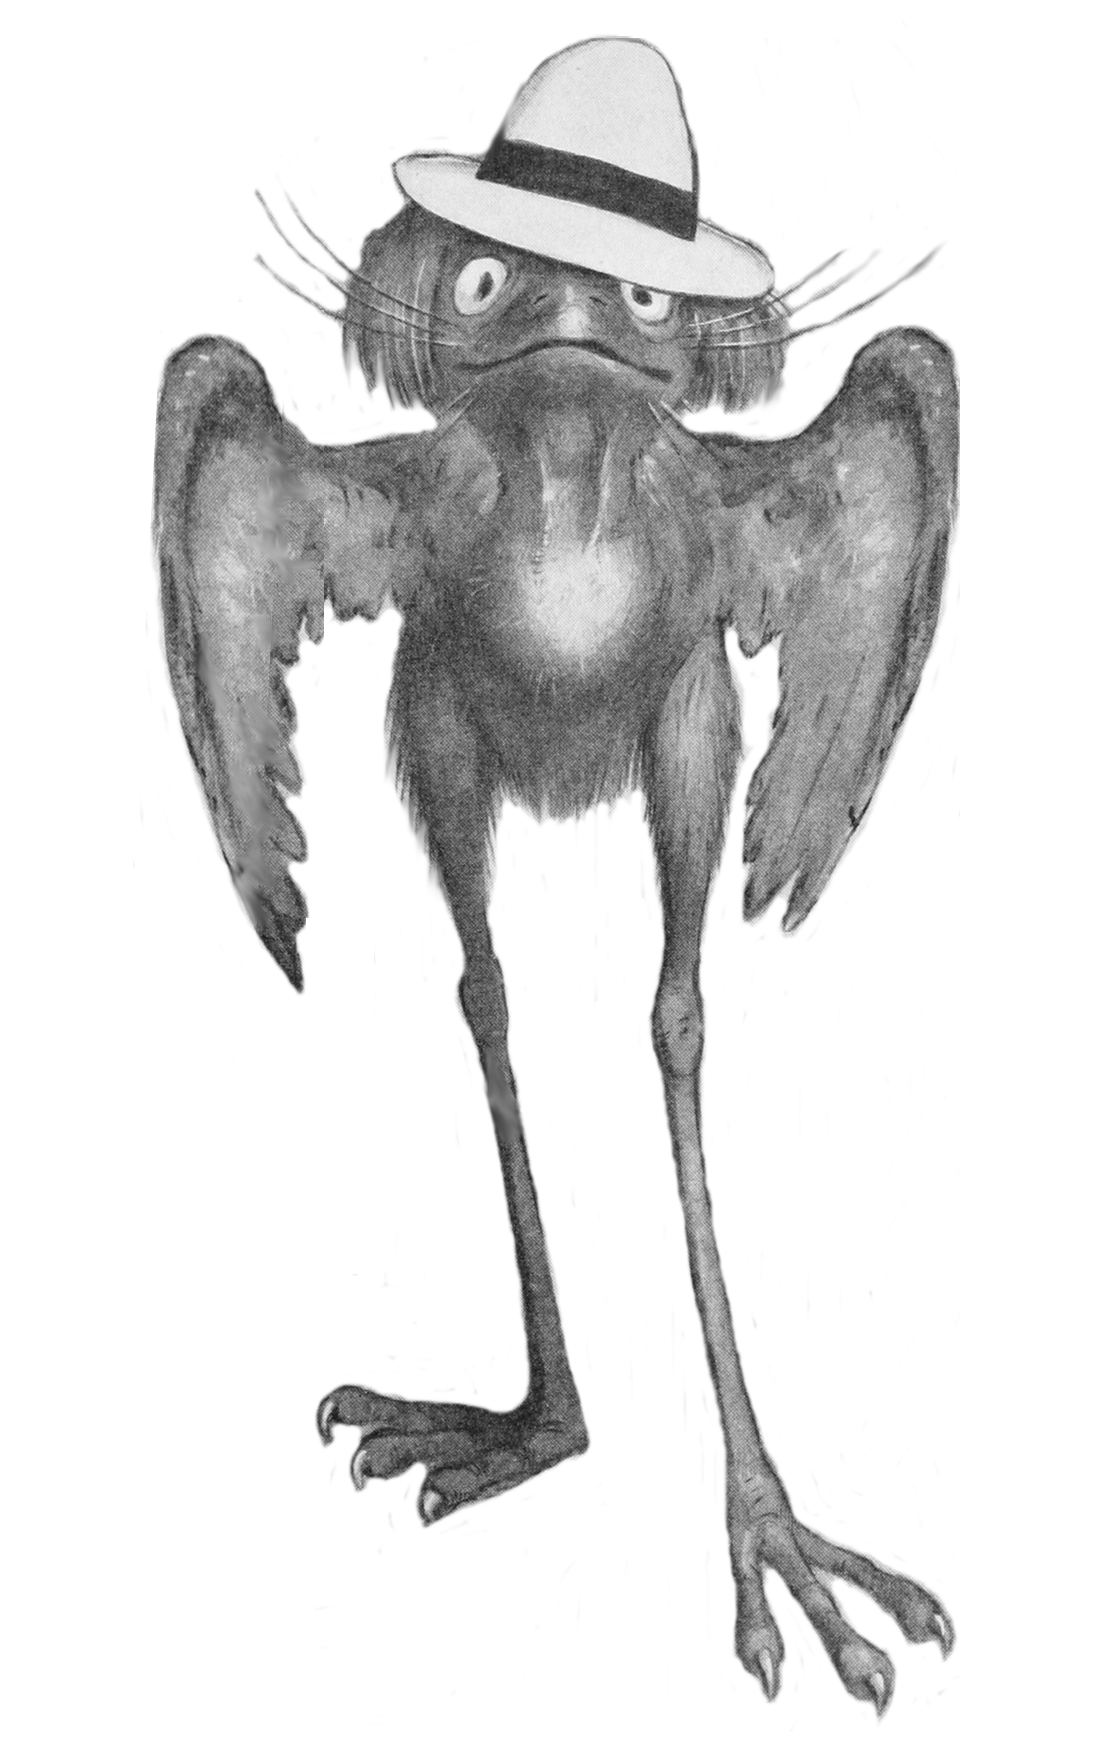
\includegraphics[scale=.1]{jubjub}
\footnote{Jubjub bird image credit: Peter Newell 1902; Daira Hopwood 2018.}
\end{center}
\vspace{-6ex}
} %notsprout

\renewcommand{\abstractname}{}
\begin{abstract}
\normalsize \noindent \textbf{Abstract.}
\defining{\Zcash} is an implementation of the \term{Decentralized Anonymous Payment scheme}
\Zerocash, with security fixes and improvements to performance and
functionality. It bridges the existing transparent payment scheme used by
\Bitcoin with a \emph{shielded} payment scheme secured by zero-knowledge
succinct non-interactive arguments of knowledge (\zkSNARKs). It attempted
to address the problem of mining centralization by use of the \Equihash
memory-hard proof-of-work algorithm.

\notsprout{\vspace{1.5ex}}
\sprout{\noindent This specification defines the \Zcash consensus protocol
as it was at launch, and explains its differences from \Zerocash and \Bitcoin.
It is a historical document and no longer specifies the current \Zcash
consensus protocol.}
\notblossom{\sapling{\noindent This specification defines the \Zcash consensus protocol
at launch; after the upgrade codenamed \Overwinter; and after the
subsequent upgrade codenamed \Sapling. It is a work in progress.
Protocol differences from \Zerocash and \Bitcoin are also explained.}}
\notheartwood{\blossom{\noindent This specification defines the \Zcash consensus protocol
at launch, and after each of the upgrades codenamed \Overwinter, \Sapling, and
\Blossom. It is a work in progress. Protocol differences from \Zerocash and
\Bitcoin are also explained.}}
\notcanopy{\heartwood{\noindent This specification defines the \Zcash consensus protocol
at launch, and after each of the upgrades codenamed \Overwinter, \Sapling, \Blossom,
and \Heartwood. It is a work in progress. Protocol differences from \Zerocash and
\Bitcoin are also explained.}}
\canopy{\noindent This specification defines the \Zcash consensus protocol
at launch, and after each of the upgrades codenamed \Overwinter, \Sapling, \Blossom,
\Heartwood, and \Canopy. It is a work in progress. Protocol differences from \Zerocash and
\Bitcoin are also explained.}

\sprout{\vspace{1ex}}\notsprout{\vspace{2.5ex}}
\noindent \textbf{Keywords:}~ \StrSubstitute[0]{\keywords}{,}{, }.

\ifxetex
\vspace{12pt}
\noindent {\setwarning
This document was built with Xe\TeX, which is \href{https://github.com/zcash/zips/issues/249}{not recommended}.
In particular, vertical spacing will be too cramped due to incorrect metrics for the Quattrocento font.}
\fi
\ifluatex
\vspace{12pt}
\noindent {\setwarning
This document was built with Lua\TeX, which is \href{https://github.com/zcash/zips/issues/249}{not recommended}.}
\fi

\end{abstract}

\sprout{\vspace{-2ex}}
\phantompart{Contents}{contents}

\renewcommand{\contentsname}{}
% <https://tex.stackexchange.com/a/182744/78411>
\renewcommand{\baselinestretch}{0.85}\normalsize
\tableofcontents
\renewcommand{\baselinestretch}{1.0}\normalsize
\newpage


\lsection{Introduction}{introduction}

\Zcash is an implementation of the \defining{\term{Decentralized Anonymous Payment scheme}
\Zerocash \cite{BCGGMTV2014}}, with security fixes and improvements
to performance and functionality. It bridges the existing
transparent payment scheme used by \defining{\Bitcoin \cite{Nakamoto2008}} with a
\emph{shielded} payment scheme secured by zero-knowledge succinct
non-interactive arguments of knowledge (\zkSNARKs).

Changes from the original \Zerocash are explained in \crossref{differences},
and highlighted in \changed{\changedcolorname} throughout the document.

\notsprout{Changes specific to the \Overwinter upgrade
are highlighted in \overwinter{\overwintercolorname}.

Changes specific to the \Sapling upgrade following \Overwinter
are highlighted in \sapling{\saplingcolorname}.

\notbeforeblossom{Changes specific to the \Blossom upgrade following \Sapling
are highlighted in \blossom{\blossomcolorname}.}

\notbeforeheartwood{Changes specific to the \Heartwood upgrade following \Blossom
are highlighted in \heartwood{\heartwoodcolorname}.}

\notbeforecanopy{Changes specific to the \Canopy upgrade following \Heartwood
are highlighted in \canopy{\canopycolorname}.}

All of these are also changes from \Zerocash.
The name \Sprout is used for the \Zcash protocol prior to \Sapling
(both before and after \Overwinter).
} %notsprout

Technical terms for concepts that play an important rôle in \Zcash are
written in \defining{\term{slanted text}}. \emph{Italics} are used for emphasis and
for references between sections of the document.

The key words \defining{\MUST, \MUSTNOT, \SHOULD,
\sprout{and \SHOULDNOT}\notsprout{\SHOULDNOT, \RECOMMENDED, \MAY, and \OPTIONAL}} in
this document are to be interpreted as described in \cite{RFC-2119} when
they appear in \defining{\ALLCAPS}. These words may also appear in this document in
lower case as plain English words, absent their normative meanings.

\vspace{2ex}
\introlist
This specification is structured as follows:

\begin{itemize}
  \item Notation — definitions of notation used throughout the document;
  \item Concepts — the principal abstractions needed to understand the protocol;
  \item Abstract Protocol — a high-level description of the protocol in terms
        of ideal cryptographic components;
  \item Concrete Protocol — how the functions and encodings of the abstract
        protocol are instantiated;
\notsprout{
  \item Network Upgrades — the strategy for upgrading the \Zcash protocol.
}
  \item Consensus Changes from \Bitcoin — how \Zcash differs from \Bitcoin at
        the consensus layer, including the Proof of Work;
  \item Differences from the \Zerocash protocol — a summary of changes from the
        protocol in \cite{BCGGMTV2014}.
\notsprout{
  \item Appendix: Circuit Design — details of how the \Sapling circuit is defined
as a \quadraticConstraintProgram.
  \item Appendix: Batching Optimizations — improvements to the efficiency of
validating multiple signatures and verifying multiple proofs.
}
\end{itemize}


\lsubsection{Caution}{caution}

\Zcash security depends on consensus. Should a program interacting with the
\Zcash network diverge from consensus, its security will be weakened or destroyed.
The cause of the divergence doesn't matter: it could be a bug in your program,
it could be an error in this documentation which you implemented as described,
or it could be that you do everything right but other software on the network
behaves unexpectedly. The specific cause will not matter to the users of your
software whose wealth is lost.

Having said that, a specification of \emph{intended} behaviour is essential
for security analysis, understanding of the protocol, and maintenance of
\Zcash and related software. If you find any mistake in this specification,
please file an issue at \url{https://github.com/zcash/zips/issues} or contact
\texttt{<security@z.cash>}.

\lsubsection{High-level Overview}{overview}

The following overview is intended to give a concise summary of the ideas
behind the protocol, for an audience already familiar with \blockChain-based
cryptocurrencies such as \Bitcoin. It is imprecise in some aspects and is not
part of the normative protocol specification. \notsprout{This overview applies
to both \Sprout and \Sapling, differences in the cryptographic constructions
used notwithstanding.}

\introsection
Value in \Zcash is either \defining{\transparent or \shielded}. Transfers of \transparent
value work essentially as in \Bitcoin and have the same privacy properties.
\xShielded value is carried by \notes\footnotewithlabel{notesandnullifiers}{In
\Zerocash \cite{BCGGMTV2014}, \notes were called
\defining{\quotedtermandindex{coins}{coins (in Zerocash)}},
and \nullifiers were called
\defining{\quotedtermandindex{serial numbers}{serial numbers (in Zerocash)}}.},
which specify an amount and \sprout{a \payingKey. The \payingKey is part of}
\notsprout{(indirectly)}
a \paymentAddress, which is a destination to which \notes can be sent.
As in \Bitcoin, this is associated with a \privateKey that can be used to
spend \notes sent to the address; in \Zcash this is called a \spendingKey.

To each \note there is cryptographically associated a \noteCommitment. Once the
\transaction creating a \note has been mined, the \note is associated with a fixed
\notePosition in a tree of \noteCommitments, and with a \nullifier\footnoteref{notesandnullifiers}
unique to that \note. Computing the \nullifier requires the associated private
\spendingKey\sapling{ (or the \nullifierDerivingKey for \Sapling{} \notes)}.
It is infeasible to correlate the \noteCommitment or \notePosition with the
corresponding \nullifier without knowledge of at least this
\sprout{\spendingKey}\notsprout{key}. An unspent valid \note, at a given point
on the \blockChain, is one for which the \noteCommitment has been publically
revealed on the \blockChain prior to that point, but the \nullifier has not.

\introlist
A \transaction can contain \transparent inputs, outputs, and scripts, which all
work as in \Bitcoin \cite{Bitcoin-Protocol}.
\sprout{
It also contains a sequence of zero or more \joinSplitDescriptions.
Each of these describes a \joinSplitTransfer\footnote{
\joinSplitTransfers in \Zcash generalize \quotedterm{Mint} and \quotedterm{Pour}
\transactions in \Zerocash; see \crossref{trstructure} for differences.}
which takes in a \transparent value and up to two input \notes, and produces a
\transparent value and up to two output \notes.
}
\notsprout{
It also includes \joinSplitDescriptions, \spendDescriptions, and \outputDescriptions.
Together these describe \defining{\shieldedTransfers} which take in \defining{\shieldedInput} \notes,
and/or produce \defining{\shieldedOutput} \notes.
(For \Sprout, each \joinSplitDescription handles up to two \shieldedInputs and
up to two \shieldedOutputs. For \Sapling, each \shieldedInput or \shieldedOutput
has its own description.)
It is also possible for value to be transferred between the \transparent and
\shielded domains.
}

The \nullifiers of the input \notes are revealed (preventing them from being
spent again) and the commitments of the output \notes are revealed (allowing
them to be spent in future).\sprout{ Each
\joinSplitDescription also includes a computationally sound \zkSNARK proof,
which proves that all of the following hold except with insignificant probability:

\begin{itemize}
  \item The input and output values balance (individually for each \joinSplitTransfer).
  \item For each input \note of nonzero value, some revealed \noteCommitment
        exists for that \note.
  \item The prover knew the private \spendingKeys of the input \notes.
  \item The \nullifiers and \noteCommitments are computed correctly.
  \item The private \spendingKeys of the input \notes are cryptographically
        linked to a signature over the whole \transaction, in such a way that
        the \transaction cannot be modified by a party who did not know these
        \privateKeys.
  \item Each output \note is generated in such a way that it is infeasible to
        cause its \nullifier to collide with the \nullifier of any other \note.
\end{itemize}
}\notsprout{ A
\transaction also includes computationally sound \zkSNARK proofs and signatures,
which prove that all of the following hold except with insignificant probability:

For each \shieldedInput,

\begin{itemize}
  \item \saplingonward{there is a revealed \valueCommitment to the same value as
        the input \note;}
  \item if the value is nonzero, some revealed \noteCommitment exists for this \note;
  \item the prover knew the \authProvingKey of the \note;
  \item the \nullifier and \noteCommitment are computed correctly.
\end{itemize}

and for each \shieldedOutput,

\begin{itemize}
  \item \saplingonward{there is a revealed \valueCommitment to the same value as
        the output \note;}
  \item the \noteCommitment is computed correctly;
  \item it is infeasible to cause the \nullifier of the output \note to collide
        with the \nullifier of any other \note.
\end{itemize}

For \Sprout, the \joinSplitStatement also includes an explicit balance check.
For \Sapling, the \valueCommitments corresponding to the inputs and outputs are
checked to balance (together with any net \transparent input or output)
outside the \zkSNARK.

In addition, various measures (differing between \Sprout and \Sapling) are
used to ensure that the \transaction cannot be modified by a party not authorized
to do so.
} %notsprout

Outside the \zkSNARK, it is \sprout{also} checked that the \nullifiers for the input
\notes had not already been revealed (i.e.\ they had not already been spent).

A \paymentAddress includes
\sprout{two \publicKeys: a \payingKey matching that of \notes sent to the address, and }a
\transmissionKey for a ``\keyPrivate'' asymmetric encryption
scheme. \defining{\mbox{\xKeyPrivate}} means that ciphertexts do not reveal information
about which key they were encrypted to, except to a holder of the corresponding
\privateKey, which in this context is called the \receivingKey. This facility is
used to communicate encrypted output \notes on the \blockChain to their
intended recipient, who can use the \receivingKey to scan the \blockChain for
\notes addressed to them and then decrypt those \notes.

\sapling{
In \Sapling, for each \spendingKey there is a \fullViewingKey that allows
recognizing both incoming and outgoing \notes without having spend authority.
This is implemented by an additional ciphertext in each \outputDescription.
}

The basis of the privacy properties of \Zcash is that when a \note is spent,
the spender only proves that some commitment for it had been revealed, without
revealing which one. This implies that a spent \note cannot be linked to the
\transaction in which it was created. That is, from an adversary's point of
view the set of possibilities for a given \note input to a \transaction{}
---its \defining{\noteTraceabilitySet}--- includes \emph{all} previous notes that the
adversary does not control or know to have been spent.\footnotewithlabel{securitycaveat}{We
make this claim only for \emph{fully shielded} \transactions. It does not exclude the
possibility that an adversary may use data present in the cleartext of a \transaction
such as the number of inputs and outputs, or metadata-based heuristics such as timing,
to make probabilistic inferences about \transaction linkage.
For consequences of this in the case of partially shielded \transactions,
see \cite{Peterson2017}, \cite{Quesnelle2017}, and \cite{KYMM2018}.} This contrasts with
other proposals for private payment systems, such as CoinJoin \cite{Bitcoin-CoinJoin}
or \CryptoNote \cite{vanSaberh2014}, that are based on mixing of a limited number of
transactions and that therefore have smaller \noteTraceabilitySets.

The \nullifiers are necessary to prevent double-spending: each \note on the
\blockChain only has one valid \nullifier, and so attempting to spend a \note
twice would reveal the \nullifier twice, which would cause the second \transaction
to be rejected.


\introsection
\lsection{Notation}{notation}

\vspace{-2ex}
$\bit$ means the type of bit values, i.e.\ $\setof{0, 1}$.
$\byte$ means the type of byte values, i.e.\ $\range{0}{255}$.

$\Nat$ means the type of nonnegative integers. $\PosInt$~means
the type of positive integers. $\Int$~means the type of integers.
$\Rat$~means the type of rationals.

$x \typecolon T$ is used to specify that $x$ has type $T$.
A cartesian product type is denoted by $S \times T$, and a function type
by $S \rightarrow T$. An argument to a function can determine other argument
or result types.

The type of a randomized algorithm is denoted by $S \rightarrowR T$.
The domain of a randomized algorithm may be $()$, indicating that it requires
no arguments. Given $f \typecolon S \rightarrowR T$ and $s \typecolon S$,
sampling a variable $x \typecolon T$ from the output of $f$ applied to $s$
is denoted by $x \leftarrowR f(s)$.

Initial arguments to a function or randomized algorithm may be
written as subscripts, e.g.\ if $x \typecolon X$, $y \typecolon Y$, and
$f \typecolon X \times Y \rightarrow Z$, then an invocation of
$f(x, y)$ can also be written $f_x(y)$.

$\setof{x \typecolon T \suchthat p_x}$ means the subset of $x$ from $T$
for which $p_x$ (a boolean expression depending on $x$) holds.

$T \subseteq U$ indicates that $T$ is an inclusive subset or subtype of $U$.
$S \union T$ means the set union of $S$ and $T$.

$S \intersection T$ means the set intersection of $S$ and $T$,
i.e.\ $\setof{x \typecolon S \suchthat x \in T}$.

\notsprout{
$S \setminus T$ means the set difference obtained by removing elements
in $T$ from $S$, i.e. $\setof{x \typecolon S \suchthat x \notin T}$.

$\fun{x \typecolon T}{e_x \typecolon U}$ means the function of type $T \rightarrow U$
mapping formal parameter $x$ to $e_x$ (an expression depending on~$x$).
The types $T$ and $U$ are always explicit.

$\exclusivefun{x \typecolon T}{e_x \typecolon U}{V}$ means
$\fun{x \typecolon T}{e_x \typecolon U \union V}$ restricted to the domain
$\setof{x \typecolon T \suchthat e_x \not\in V}$ and range $U$.

$\powerset{T}$ means the powerset of $T$.
}

$\typeexp{T}{\ell}$, where $T$ is a type and $\ell$ is an integer,
means the type of sequences of length $\ell$ with elements in $T$. For example,
$\bitseq{\ell}$ means the set of sequences of $\ell$ bits, and
$\byteseq{k}$ means the set of sequences of $k$ bytes.

$\byteseqs$ means the type of byte sequences of arbitrary length.

$\length(S)$ means the length of (number of elements in) $S$.

\notsprout{
$\truncate{k}(S)$ means the sequence formed from the first $k$ elements of $S$.
}

$\hexint{}$ followed by a string of $\mathtt{monospace}$ hexadecimal
digits means the corresponding integer converted from hexadecimal.
\notsprout{$\zerobytes{\ell}$ means the sequence of $\ell$ zero bytes.}

$\ascii{...}$ means the given string represented as a
sequence of bytes in US-ASCII. For example, $\ascii{abc}$ represents the
byte sequence $\hexarray{61,62,63}$.

$\zeros{\ell}$ means the sequence of $\ell$ zero bits.
\notsprout{$\ones{\ell}$ means the sequence of $\ell$ one bits.}

$a..b$, used as a subscript, means the sequence of values
with indices $a$ through $b$ inclusive. For example,
$\AuthPublicNew{\allNew}$ means the sequence
$\vphantom{\mathsf{a_a}}\smash{[\AuthPublicNew{\mathrm{1}}, \AuthPublicNew{\mathrm{2}}, ...\,\AuthPublicNew{\NNew}]}$.
(For consistency with the notation in \cite{BCGGMTV2014} and in \cite{BK2016},
this specification uses 1-based indexing and inclusive ranges,
\raisedstrut notwithstanding the compelling arguments to the contrary made in
\cite{EWD-831}.)

$\range{a}{b}$ means the set or type of integers from $a$ through
$b$ inclusive.

$\listcomp{f(x) \for x \from a \upto b}$ means the sequence
formed by evaluating $f$ on each integer from $a$ to $b$ inclusive, in
ascending order. Similarly, $\listcomp{f(x) \for x \from a \downto b}$ means
the sequence formed by evaluating $f$ on each integer from $a$ to $b$
inclusive, in descending order.

$a \bconcat b$ means the concatenation of sequences $a$ then $b$.

$\concatbits(S)$ means the sequence of bits obtained by
concatenating the elements of $S$ viewed as bit sequences. If the
elements of $S$ are byte sequences, they are converted to bit sequences
with the \emph{most significant} bit of each byte first.

$\sorted(S)$ means the sequence formed by sorting the elements
of $S$.

$\GF{n}$ means the finite field with $n$ elements, and
$\GFstar{n}$ means its group under multiplication (which excludes $0$).

Where there is a need to make the distinction, we denote the unique
representative of $a \typecolon \GF{n}$ in the range $\range{0}{n-1}$
(or the unique representative of $a \typecolon \GFstar{n}$ in the range
$\range{1}{n-1}$) as $a \bmod n$. Conversely, we denote the element
of $\GF{n}$ corresponding to an integer $k \typecolon \Int$
as $k \pmod{n}$. We also use the latter notation in the context of
an equality $k = k' \pmod{n}$ as shorthand for $k \bmod n = k' \bmod n$,
and similarly $k \neq k' \pmod{n}$ as shorthand for $k \bmod n \neq k' \bmod n$.
(When referring to constants such as $0$ and $1$ it is usually not
necessary to make the distinction between field elements and their
representatives, since the meaning is normally clear from context.)

$\GF{n}[z]$ means the ring of polynomials over $z$ with coefficients
in $\GF{n}$.

$a + b$ means the sum of $a$ and $b$. This may refer to addition of
integers, rationals, finite field elements, or group elements
(see \crossref{abstractgroup}) according to context.

$-a$ means the value of the appropriate integer, rational,
finite field, or group type such that $(-a) + a = 0$
(or when $a$ is an element of a group $\GroupG{}$, $(-a) + a = \ZeroG{}$),
and $a - b$ means $a + (-b)$.

$a \mult b$ means the product of multiplying $a$ and $b$.
This may refer to multiplication of integers, rationals, or
finite field elements according to context (this notation is not
used for group elements).

$a / b$, also written $\hfrac{a}{b}$, means the value of the
appropriate integer, rational, or finite field type such that
$(a / b) \mult b = a$.

$a \bmod q$, for $a \typecolon \Nat$ and $q \typecolon \PosInt$,
means the remainder on dividing $a$ by $q$. (This usage does not
conflict with the notation above for the unique representative of
a field element.)

$a \xor b$ means the bitwise-exclusive-or of $a$ and $b$,
and $a \band b$ means the bitwise-and of $a$ and $b$. These are
defined on integers or (equal-length) bit sequences according to context.

\vspace{-0.5ex}
$\!\vsum{i=1}{\rmN} a_i$ means the sum of $a_{\allN{}}$.\;
$\vproduct{i=1}{\rmN} a_i$ means the product of $a_{\allN{}}$.\;
$\vxor{i=1}{\rmN} a_i$ means the bitwise exclusive-or of $a_{\allN{}}$.

When $N = 0$ these yield the appropriate neutral element, i.e.
$\ssum{i=1}{0} a_i = 0$, $\sproduct{i=1}{0} a_i = 1$, and
$\sxor{i=1}{0} a_i = 0$ or the all-zero bit sequence of length given
by the type of $a$.

\notsprout{
$\possqrt{a}$, where $a \typecolon \GF{q}$, means the positive square root
of $a$ in $\GF{q}$, i.e.\ in the range $\bigrange{0}{\hfrac{q-1}{2}}$.
It is only used in cases where the square root must exist.

$\optsqrt{a}$, where $a \typecolon \GF{q}$, means an arbitrary
square root of $a$ in $\GF{q}$, or $\bot$ if no such square root exists.

$b \bchoose x : y$ means $x$ when $b = 1$, or $y$ when $b = 0$.
}

$a^b$, for $a$ an integer or finite field element and
$b \typecolon \Int$, means the result of raising $a$ to the exponent $b$,
i.e.
\begin{formulae}
  \item $a^b := \begin{cases}
          \sproduct{i=1}{b}  \kern 0.15em a, &\caseif b \geq 0 \\[1.5ex]
          \sproduct{i=1}{-b} \kern 0.1em \hfrac{1}{a}, &\caseotherwise.
        \end{cases}$
\end{formulae}

The $\scalarmult{k}{P}$ notation for scalar multiplication in a group is
defined in \crossref{abstractgroup}.

The convention of affixing $\Repr$ to a variable name is used
for variables that denote bit-sequence representations of group elements.

The binary relations $<$, $\leq$, $=$, $\geq$, and $>$ have their conventional
meanings on integers and rationals, and are defined lexicographically on
sequences of integers.

$\floor{x}$ means the largest integer $\leq x$.
$\ceiling{x}$ means the smallest integer $\geq x$.

$\bitlength(x)$, for $x \typecolon \Nat$, means the smallest integer
$\ell$ such that $2^\ell > x$.

The symbol $\bot$ is used to indicate unavailable information, or a failed
decryption or validity check.

\introlist
The following integer constants will be instantiated in \crossref{constants}:
\begin{formulae}
  \item \begin{flushleft}
    $\MerkleDepthSprout$,\sapling{ $\MerkleDepthSapling$,} $\NOld$, $\NNew$,
    $\ValueLength$, $\MerkleHashLengthSprout$,\sapling{ $\MerkleHashLengthSapling$,}
    $\hSigLength$, $\PRFOutputLengthSprout$,\sapling{ $\PRFOutputLengthExpand$, $\PRFOutputLengthNfSapling$,}
    $\NoteCommitRandLength$, \changed{$\RandomSeedLength$,} $\AuthPrivateLength$,
    \changed{$\NoteAddressPreRandLength$,}\sapling{ $\SpendingKeyLength$, $\DiversifierLength$,
    $\InViewingKeyLength$, $\OutViewingKeyLength$, $\ScalarLength$,}
    $\MAXMONEY$,\blossom{ $\BlossomActivationHeight$,}\canopy{ $\CanopyActivationHeight$, $\ZIPTwoOneTwoGracePeriod$}
    $\SlowStartInterval$, $\PreBlossomHalvingInterval$, $\MaxBlockSubsidy$, $\NumFounderAddresses$,
    $\PoWLimit$, $\PoWAveragingWindow$, $\PoWMedianBlockSpan$, $\PoWDampingFactor$,
    \notblossom{and }$\PreBlossomPoWTargetSpacing$\blossom{, and $\PostBlossomPoWTargetSpacing$}.
  \end{flushleft}
\end{formulae}

\sprout{The bit sequence constant $\UncommittedSprout \typecolon \bitseq{\MerkleHashLengthSprout}$,}
\notsprout{The bit sequence constants $\UncommittedSprout \typecolon \bitseq{\MerkleHashLengthSprout}$
\sapling{and $\UncommittedSapling \typecolon \bitseq{\MerkleHashLengthSapling}$},}
and rational constants $\FoundersFraction$, $\PoWMaxAdjustDown$, and
$\PoWMaxAdjustUp$ will also be defined in that section.

\notsprout{
We use the abbreviation ``\defining{\xCtEdwards}'' to refer to \completeTwistedEdwardsEllipticCurves and
coordinates (see \crossref{jubjub}).
}


\intropart
\lsection{Concepts}{concepts}

\lsubsection{Payment Addresses and Keys}{addressesandkeys}

Users who wish to receive payments in the \Zcash protocol must have a
\defining{\paymentAddress, which is generated from a \spendingKey.}

\introlist
The following diagram depicts the relations between key
components\notsprout{ in \Sprout}\sapling{ and \Sapling}.
Arrows point from a component to any other component(s) that can be derived
from it. Double lines indicate that the same component is used in multiple
abstractions.

\begin{center}
\sprout{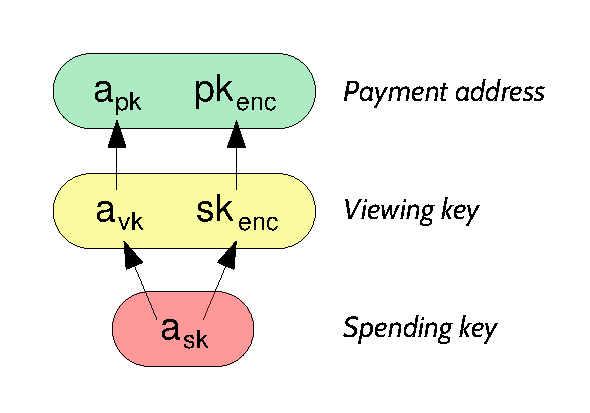
\includegraphics[scale=.7]{key_components}}
\sapling{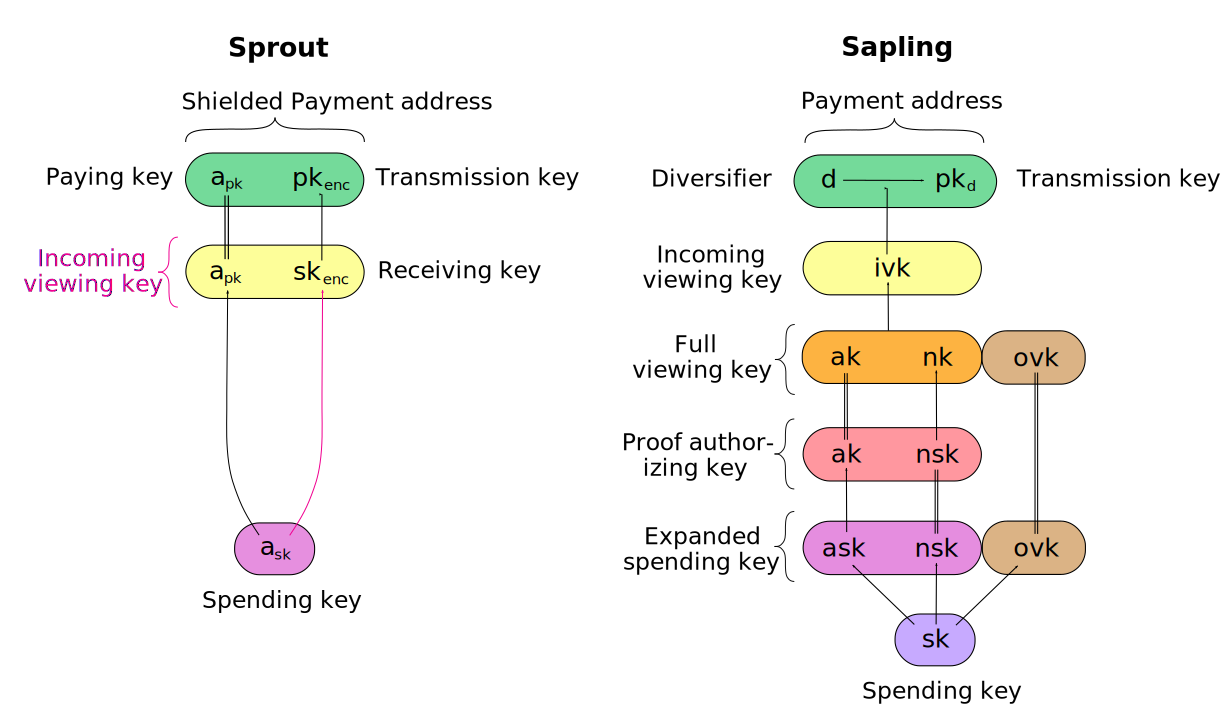
\includegraphics[scale=.5]{key_components_sapling}}
\end{center}

\sproutspecific{
\defining{The \receivingKey $\TransmitPrivate$, \incomingViewingKey
$\InViewingKey = (\AuthPublic, \TransmitPrivate)$, and \paymentAddress
$\PaymentAddress = (\AuthPublic, \TransmitPublic)$ are derived from the
\spendingKey $\AuthPrivate$, as described in \crossref{sproutkeycomponents}.}
} %sproutspecific

\saplingonward{
\defining{An \expandedSpendingKey is composed of a \authSigningKey $\AuthSignPrivate$,
a \authNullifierKey $\AuthProvePrivate$, and an \outgoingViewingKey $\OutViewingKey$.
From these components we can derive an \authProvingKey $(\AuthSignPublic, \AuthProvePrivate)$,
a \fullViewingKey $(\AuthSignPublic, \AuthProvePublic, \OutViewingKey)$,
an \incomingViewingKey $\InViewingKey$, and a set of \diversifiedPaymentAddresses
$\DiversifiedPaymentAddress = (\Diversifier, \DiversifiedTransmitPublic)$,
as described in \crossref{saplingkeycomponents}.

The consensus protocol does not depend on how an \expandedSpendingKey is constructed.
Two methods of doing so are defined:
\begin{enumerate}
  \item Generate a \spendingKey $\SpendingKey$ at random and derive the \expandedSpendingKey
        $(\AuthSignPrivate, \AuthProvePrivate, \OutViewingKey)$ from it, as shown in the
        diagram above and described in \crossref{saplingkeycomponents}.
  \item Obtain an \extendedSpendingKey as specified in \cite{ZIP-32}; this includes a superset
        of the components of an \expandedSpendingKey. This method is used in the context of a
        \hdWallet.
\end{enumerate}
} %saplingonward

\vspace{-2ex}
\nnote{In \zcashd, all \Sapling keys and addresses are derived according to \cite{ZIP-32}.}
} %saplingonward

\vspace{2ex}
The composition of \paymentAddresses, \changed{\incomingViewingKeys,}
\sapling{\fullViewingKeys,} and \spendingKeys is a cryptographic protocol
detail that should not normally be exposed to users. However, user-visible
operations should be provided to obtain a
\paymentAddress\changed{ or \incomingViewingKey}\sapling{ or \fullViewingKey}
from a \spendingKey or \extendedSpendingKey.

Users can accept payment from multiple parties with a single \paymentAddress
and the fact that these payments are destined to
the same payee is not revealed on the \blockChain, even to the
paying parties. \emph{However} if two parties collude to compare a
\paymentAddress they can trivially determine they are the same. In the
case that a payee wishes to prevent this they should create a distinct
\paymentAddress for each payer.

\saplingonward{
\Sapling provides a mechanism to allow the efficient creation of
\diversifiedPaymentAddresses with the same spending authority. A group of
such addresses shares the same \fullViewingKey and \incomingViewingKey, and
so creating as many unlinkable addresses as needed does not increase the cost
of scanning the \blockChain for relevant \transactions.
} %saplingonward

\vspace{-1ex}
\pnote{
It is conventional in cryptography to refer to the key used to encrypt
a message in an asymmetric encryption scheme as the ``\defining{\publicKey}''.
However, the \publicKey used as \defining{the \transmissionKey component of an address
($\TransmitPublic$\sapling{ or $\DiversifiedTransmitPublic$})} need not be
publically distributed; it has the same distribution as the \paymentAddress itself.
As mentioned above, limiting the distribution of the \paymentAddress is important
for some use cases. This also helps to reduce reliance of the overall protocol
on the security of the cryptosystem used for \note encryption
(see \crossref{sproutinband}\sapling{ and \crossref{saplinginband}}),
since an adversary would have to know
$\TransmitPublic$\sapling{ or some $\DiversifiedTransmitPublic$}
in order to exploit a hypothetical weakness in that cryptosystem.
}

\introsection
\lsubsection{Notes}{notes}

\sprout{
A \defining{\note} (denoted $\NoteTuple{}$) is a tuple $\changed{(\AuthPublic, \Value,
\NoteAddressRand, \NoteCommitRand)}$. It represents that a value $\Value$ is
spendable by the recipient who holds the \spendingKey $\AuthPrivate$ corresponding
to $\AuthPublic$, as described in the previous section.
} %sprout
\notsprout{
A \defining{\note} (denoted $\NoteTuple{}$) can be a \Sprout{} \note\sapling{ or a
\Sapling{} \note}. In either case it represents that a value $\Value$ is
spendable by the recipient who holds the \spendingKey corresponding
to a given \paymentAddress.
} %notsprout

Let \sprout{$\MAXMONEY$ and $\PRFOutputLengthSprout$}
\notsprout{$\MAXMONEY$, $\PRFOutputLengthSprout$\sapling{, $\PRFOutputLengthNfSapling$, and $\DiversifierLength$}}
be as defined in \crossref{constants}.

Let $\NoteCommitSproutAlg$ be as defined in \crossref{concretesproutnotecommit}.

\sapling{
Let $\NoteCommitSaplingAlg$ be as defined in \crossref{concretesaplingnotecommit}.

Let $\KASapling$ be as defined in \crossref{concretesaplingkeyagreement}.
} %sapling

\vspace{2ex}
\introlist
A \SproutOrNothing{} \note is a tuple $\changed{(\AuthPublic,
\Value, \NoteAddressRand, \NoteCommitRand)}$, where:
\begin{itemize}
  \item $\AuthPublic \typecolon \PRFOutputSprout$ is the \defining{\payingKey} of the
        recipient's \paymentAddress;
  \item $\Value \typecolon \range{0}{\MAXMONEY}$ is an integer
        representing the value of the \note in \zatoshi
        (\defining{$1$ \ZEC = $10^8$ \zatoshi});
  \item $\NoteAddressRand \typecolon \PRFOutputSprout$
        is used as input to $\PRFnf{\AuthPrivate}$ to derive the
        \nullifier of the \note;
  \item $\NoteCommitRand \typecolon \NoteCommitSproutTrapdoor$
        is a random \commitmentTrapdoor as defined in \crossref{abstractcommit}.
\end{itemize}

\introlist
Let $\NoteTypeSprout$ be the type of a \SproutOrNothing{} \note, i.e.
\begin{formulae}
  \item $\NoteTypeSprout := \changed{\PRFOutputSprout \times \range{0}{\MAXMONEY} \times \PRFOutputSprout
           \times \NoteCommitSproutTrapdoor}$.
\end{formulae}

\sapling{
\vspace{1ex}
\introlist
A \Sapling{} \note is a tuple $(\Diversifier, \DiversifiedTransmitPublic,
\Value, \NoteCommitRand)$, where:
\begin{itemize}
  \item $\Diversifier \typecolon \DiversifierType$
        is the \diversifier of the recipient's \paymentAddress;
  \item $\DiversifiedTransmitPublic \typecolon \KASaplingPublicPrimeSubgroup$
        is the \diversifiedTransmissionKey of the recipient's \paymentAddress;
  \item $\Value \typecolon \range{0}{\MAXMONEY}$ is an integer
        representing the value of the \note in \zatoshi;
  \item $\NoteCommitRand \typecolon \NoteCommitSaplingTrapdoor$
        is a random \commitmentTrapdoor as defined in \crossref{abstractcommit}.
\end{itemize}

\introlist
Let $\NoteTypeSapling$ be the type of a \Sapling{} \note, i.e.
\begin{formulae}
  \item $\NoteTypeSapling := \DiversifierType \times \KASaplingPublicPrimeSubgroup \times \range{0}{\MAXMONEY}
           \times \NoteCommitSaplingTrapdoor$.
\end{formulae}
} %sapling

Creation of new \notes is described in \crossref{send}. When \notes are sent,
only a commitment (see \crossref{abstractcommit}) to the above values is disclosed
publically, and added to a data structure called the \noteCommitmentTree.
This allows the value and recipient to be kept private, while the commitment is
used by the \zkSNARKProof when the \note is spent, to check that it exists
on the \blockChain.

\vspace{2ex}
\introlist
A \SproutOrNothing{} \defining{\noteCommitment} on a \note
$\NoteTuple{} = \changed{(\AuthPublic, \Value, \NoteAddressRand, \NoteCommitRand)}$ is computed as

\begin{formulae}
  \item $\NoteCommitmentSprout(\NoteTuple{}) =
          \NoteCommitSprout{\NoteCommitRand}(\AuthPublic, \Value, \NoteAddressRand)$,
\end{formulae}
\vspace{-1.5ex}
where $\NoteCommitSprout{}$ is instantiated in \crossref{concretesproutnotecommit}.


\sapling{
\vspace{2ex}
\introlist
Let $\DiversifyHash$ be as defined in \crossref{concretediversifyhash}.

A \Sapling{} \defining{\noteCommitment} on a \note
$\NoteTuple{} = (\Diversifier, \DiversifiedTransmitPublic, \Value, \NoteCommitRand)$ is computed as

\begin{formulae}
  \item $\DiversifiedTransmitBase := \DiversifyHash(\Diversifier)$
        \vspace{-1ex}
  \item $\NoteCommitmentSapling(\NoteTuple{}) := \begin{cases}
          \bot, &\caseif \DiversifiedTransmitBase = \bot \\
          \NoteCommitSapling{\NoteCommitRand}(\reprJ\Of{\DiversifiedTransmitBase},
                                              \reprJ\Of{\DiversifiedTransmitPublic},
                                              \Value), &\caseotherwise.
        \end{cases}$
\end{formulae}
\vspace{-1.5ex}
where $\NoteCommitSapling{}$ is instantiated in \crossref{concretewindowedcommit}.

Notice that the above definition of a \Sapling{} \note does not have a
$\NoteAddressRand$ field. There is in fact a $\NoteAddressRand$ value associated
with each \Sapling{} \note, but this can only be computed once its position in the
\noteCommitmentTree is known (see \crossref{transactions} and \crossref{merkletree}).
We refer to the combination of a \note and its \notePosition $\NotePosition$, as a
\positionedNote.

For a \positionedNote, we can compute the value
$\NoteAddressRand$ as described in \crossref{commitmentsandnullifiers}.
} %sapling

\vspace{2ex}
A \nullifier (denoted $\nf$) is derived from the $\NoteAddressRand$ value
of a \note and the recipient's
\spendingKey $\AuthPrivate$\sapling{ or \defining{\nullifierDerivingKey} $\AuthProvePublic$}.
This computation uses a \pseudoRandomFunction (see \crossref{abstractprfs}),
as described in \crossref{commitmentsandnullifiers}.

A \note is spent by proving knowledge of
$(\NoteAddressRand, \AuthPrivate)$\sapling{ or $(\NoteAddressRand, \AuthSignPublic, \AuthProvePrivate)$}
in zero knowledge while publically disclosing its \nullifier $\nf$,
allowing $\nf$ to be used to prevent double-spending. \sapling{In the case
of \Sapling, a \spendAuthSignature is also required, in order to demonstrate
knowledge of $\AuthSignPrivate$.}


\lsubsubsection{Note Plaintexts and Memo Fields}{noteptconcept}

Transmitted \notes are stored on the \blockChain in encrypted form, together with
a representation of the \noteCommitment $\cm$.

The \notePlaintexts in each \joinSplitDescription are encrypted to the
respective \transmissionKeys $\TransmitPublicNew{\allNew}$.

\introlist
Each \SproutOrNothing{} \defining{\notePlaintext} (denoted $\NotePlaintext{}$) consists of

\vspace{-1ex}
\begin{formulae}
  \item $(\changed{\NotePlaintextLeadByte \typecolon \byte,\ }
          \Value \typecolon \ValueType, \NoteAddressRand \typecolon \PRFOutputSprout,
          \NoteCommitRand \typecolon \NoteCommitSproutTrapdoor\changed{, \Memo \typecolon \MemoType})$.
\end{formulae}

\saplingonward{
The \notePlaintext in each \outputDescription is encrypted to the
\diversifiedPaymentAddress $(\Diversifier, \DiversifiedTransmitPublic)$.

\introlist
Each \Sapling{} \defining{\notePlaintext} (denoted $\NotePlaintext{}$) consists of

\begin{formulae}
  \item $(\NotePlaintextLeadByte \typecolon \byte,
          \Diversifier \typecolon \DiversifierType, \Value \typecolon \ValueType,
          \NoteCommitRandBytesOrSeedBytes \typecolon \NoteSeedBytesType, \Memo \typecolon \MemoType)$
\end{formulae}

The fields \notcanopy{$\Diversifier$, $\Value$, and $\NoteCommitRandBytes$}\notbeforecanopy{$\Diversifier$ and $\Value$}
are as defined in \crossref{notes}.

\canopy{
The field $\NoteSeedBytes$ is described in \crossref{saplingsend}.
} %canopy
} %saplingonward

\changed{
$\Memo$ represents a $\MemoByteLength$-byte \defining{\memo} associated with this \note.
The usage of the \memo is by agreement between the sender and recipient of the \note.
}

Encodings are given in \crossref{notept}.
The result of encryption forms part of a \noteOrNotesCiphertext.
For further details, see \crossref{sproutinband}\sapling{ and \crossref{saplinginband}}.


\lsubsection{The Block Chain}{blockchain}

At a given point in time, each \defining{\fullValidator} is aware of a set of candidate
\blocks. These form a tree rooted at the \genesisBlock, where each node
in the tree refers to its parent via the $\hashPrevBlock$ \blockHeader field
(see \crossref{blockheader}).

A path from the root toward the leaves of the tree consisting of a sequence
of one or more valid \blocks consistent with consensus rules, is called a
\defining{\validBlockChain}.

Each \block in a \defining{\blockChain} has a \defining{\blockHeight}. The \blockHeight
of the \defining{\genesisBlock} is $0$, and the \blockHeight of each subsequent \block
in the \blockChain increments by $1$.

In order to choose the \defining{\bestValidBlockChain} in its view of the
overall \block tree, a node sums the work, as defined in \crossref{workdef}, of
all \blocks in each \validBlockChain, and considers the \validBlockChain with greatest
total work to be best. To break ties between leaf \blocks, a node will prefer the
\block that it received first.

The consensus protocol is designed to ensure that for any given \blockHeight,
the vast majority of nodes should eventually agree on their \bestValidBlockChain
up to that height.


\lsubsection{Transactions and Treestates}{transactions}

Each \block contains one or more \defining{\transactions}.

\defining{\xTransparentInputs} to a \transaction insert value into a \defining{\transparentTxValuePool}
associated with the \transaction, and \defining{\transparentOutputs} remove value from this pool.
As in \Bitcoin, the remaining value in the pool is available to miners as a fee.

\vspace{-3ex}
\consensusrule{
The remaining value in the \transparentTxValuePool{} \MUST be nonnegative.
}
\vspace{2ex}

\introlist
\sprout{To each \transaction there is associated an initial \defining{\treestate}.
A \treestate consists of:}
\notsprout{To each \transaction there are associated initial \defining{\treestates}
for \Sprout\sapling{ and for \Sapling}. \sapling{Each} \treestate consists of:}

\begin{itemize}
  \item a \noteCommitmentTree (\crossref{merkletree});
  \item a \nullifierSet (\crossref{nullifierset}).
\end{itemize}

Validation state associated with \transparent inputs and outputs, such as the UTXO
(Unspent Transaction Output) set, is not described in this document; it is
used in essentially the same way as in \Bitcoin.

An \defining{\anchor} is a Merkle tree root of a \noteCommitmentTree\sapling{ (either the
\Sprout tree or the \Sapling tree)}. It uniquely identifies a \noteCommitmentTree
state given the assumed security properties of the Merkle tree's
\hashFunction. Since the \nullifierSet is always updated together with the
\noteCommitmentTree, this also identifies a particular state of the associated
\nullifierSet.

\introlist
In a given \blockChain, \sapling{for each of \Sprout and \Sapling,}
\treestates are chained as follows:

\begin{itemize}
  \item The input \treestate of the first \block is the empty \treestate.
  \item The input \treestate of the first \transaction of a \block is the final
        \treestate of the immediately preceding \block.
  \item The input \treestate of each subsequent \transaction in a \block is the
        output \treestate of the immediately preceding \transaction.
  \item The final \treestate of a \block is the output \treestate of its last
        \transaction.
\end{itemize}

\changed{\joinSplitDescriptions also have interstitial input and output
\treestates\notsprout{ for \Sprout}, explained in the following section.}
\sapling{There is no equivalent of interstitial \treestates for \Sapling.}


\lsubsection{JoinSplit Transfers and Descriptions}{joinsplit}

A \defining{\joinSplitDescription} is data included in a \transaction that describes a
\defining{\joinSplitTransfer}, i.e.\ a \shielded value transfer.
\sprout{This kind of value transfer is}
\notsprout{In \Sprout, this kind of value transfer was}
the primary \Zcash-specific operation performed by \transactions.

A \joinSplitTransfer spends $\NOld$ \notes $\nOld{\allOld}$ and \transparent input
$\vpubOld$, and creates $\NNew$ \notes $\nNew{\allNew}$ and \transparent output
$\vpubNew$.
It is associated with a \joinSplitStatement instance (\crossref{joinsplitstatement}),
for which it provides a \zkSNARKProof.

Each \transaction has a \sequenceOfJoinSplitDescriptions{}.

The \changed{total $\vpubNew$ value adds to, and the total} $\vpubOld$
value subtracts from the \transparentTxValuePool of the containing \transaction.

The \anchor of each \joinSplitDescription in a \transaction{} refers to a
\SproutOrNothing{} \treestate.

For each of the $\NOld$ \shieldedInputs, a \nullifier is revealed. This allows
detection of double-spends as described in \crossref{nullifierset}.

\changed{
For each \joinSplitDescription in a \transaction, an interstitial output \treestate is
constructed which adds the \noteCommitments and \nullifiers specified in that
\joinSplitDescription to the input \treestate referred to by its \anchor.
This interstitial output \treestate is available for use as the \anchor of subsequent
\joinSplitDescriptions in the same \transaction. In general, therefore, the set
of interstitial \treestates associated with a \transaction forms a tree in which
the parent of each node is determined by its \anchor.

Interstitial \treestates are necessary because when a \transaction is constructed,
it is not known where it will eventually appear in a mined \block. Therefore the
\anchors that it uses must be independent of its eventual position.
}

\begin{consensusrules}
  \item The input and output values of each \joinSplitTransfer{} \MUST balance
        exactly.
  \item For the first \joinSplitDescription of a \transaction, the \anchor{} \MUST
        be the output \SproutOrNothing{} \treestate of a previous \block.
\changed{
  \item The \anchor of each \joinSplitDescription in a \transaction{} \MUST refer
        to either some earlier \block's final \SproutOrNothing{} \treestate, or to
        the interstitial output \treestate of any prior \joinSplitDescription in
        the same \transaction.
}
\end{consensusrules}


\sapling{
\lsubsection{Spend Transfers, Output Transfers, and their Descriptions}{spendsandoutputs}

\joinSplitTransfers are not used for \Sapling{} \notes. \defining{Instead, there is a
separate \spendTransfer for each \shieldedInput, and a separate \outputTransfer
for each \shieldedOutput.}

\defining{\spendDescriptions and \outputDescriptions} are data included in a transaction
that describe \spendTransfers and \outputTransfers, respectively.

A \spendTransfer spends a \note $\nOld{}$. Its \spendDescription includes a
\defining{\xPedersenValueCommitment} to the value of the \note.
It is associated with an instance of a \spendStatement (\crossref{spendstatement})
for which it provides a \zkSNARKProof.

An \outputTransfer creates a \note $\nNew{}$. Similarly, its \outputDescription
includes a \xPedersenValueCommitment to the \note value.
It is associated with an instance of an \outputStatement (\crossref{outputstatement})
for which it provides a \zkSNARKProof.

Each \transaction has a sequence of \spendDescriptions and a sequence of
\outputDescriptions.

To ensure balance, we use a homomorphic property of \xPedersenCommitments that
allows them to be added and subtracted, as elliptic curve points (\crossref{concretehomomorphiccommit}).
The result of adding two \xPedersenValueCommitments, committing to values $\Value_1$ and
$\Value_2$, is a new \xPedersenValueCommitment that commits to $\Value_1 + \Value_2$.
Subtraction works similarly.

Therefore, balance can be enforced by adding all of the \defining{\valueCommitments} for
\shieldedInputs, subtracting all of the \valueCommitments for \shieldedOutputs,
and proving by use of a \bindingSignature (as described in \crossref{bindingsig})
that the result commits to a value consistent with the net \transparent value change.
This approach allows all of the \zkSNARK \statements to be independent of
each other, potentially increasing opportunities for precomputation.

A \spendDescription includes an \anchor, which refers to the output
\Sapling{} \treestate of a previous \block. It also reveals a \nullifier,
which allows detection of double-spends as described in \crossref{nullifierset}.

\vspace{-1ex}
\nnote{
Interstitial \treestates are not necessary for \Sapling, because a \spendTransfer
in a given \transaction cannot spend any of the \shieldedOutputs of the same
\transaction. This is not an onerous restriction because, unlike \Sprout where
each \joinSplitTransfer must balance individually, in \Sapling it is only necessary
for the whole \transaction to balance.
}

\begin{consensusrules}
  \item The \transaction{} \MUST balance as specified in \crossref{saplingbalance}.
  \item The \anchor of each \spendDescription{} \MUST refer to some earlier \block's final
        \Sapling{} \treestate.
\end{consensusrules}
} %sapling


\lsubsection{Note Commitment Trees}{merkletree}

\vspace{-2ex}
\begin{center}
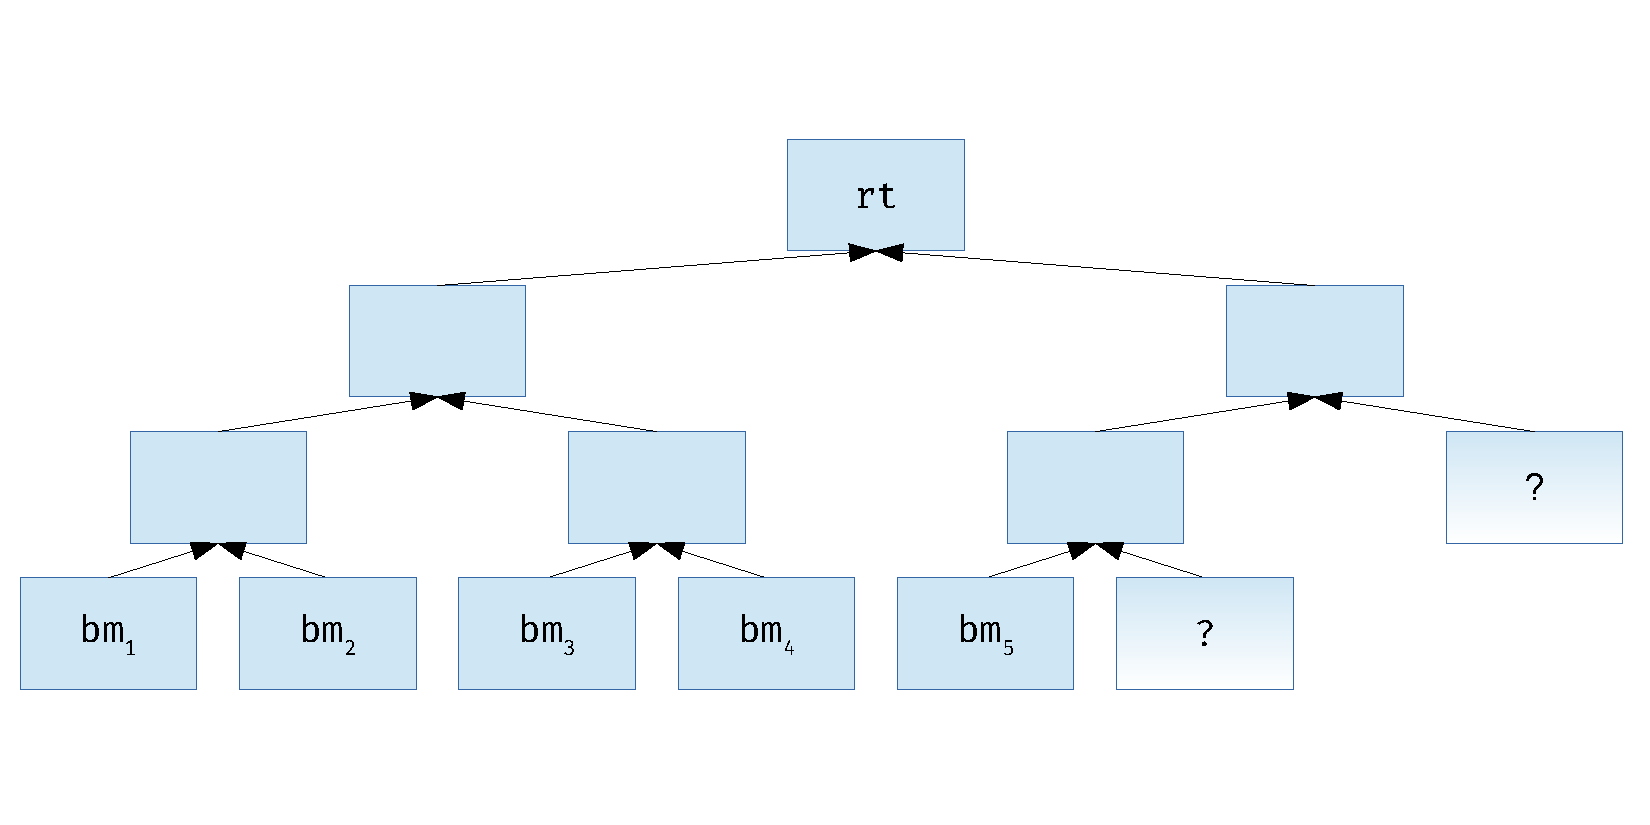
\includegraphics[scale=.4]{incremental_merkle}
\end{center}
\vspace{-2ex}

\defining{A \noteCommitmentTree is an \incrementalMerkleTree} of fixed depth used to store
\noteCommitments that \joinSplitTransfers\sapling{ or \spendTransfers} produce.
Just as the \defining{\utxoSet} (UTXO set) used in \Bitcoin,
it is used to express the existence of value and the capability to spend it.
However, unlike the UTXO set, it is \emph{not} the job of this tree to protect
against double-spending, as it is append-only.

A \defining{\merkleRoot} of a \noteCommitmentTree is associated with each \treestate
(\crossref{transactions}).

Each \defining{\merkleNode} in the \incrementalMerkleTree is associated with a
\defining{\merkleHash} of size $\MerkleHashLengthSprout$ \sapling{ or $\MerkleHashLengthSapling$} bits.
The \defining{\merkleLayer} numbered $h$, counting from \merkleLayer $0$ at the \merkleRoot, has
$2^h$ \merkleNodes with \defining{\merkleIndices} $0$ to $2^h-1$ inclusive.
The \defining{\merkleHash} associated with the \merkleNode at \merkleIndex $i$ in \merkleLayer $h$
is denoted $\MerkleNode{h}{i}$.

The \merkleIndex of a \notesCommitment at the leafmost layer
($\MerkleDepthSproutOrSapling$) is called its \defining{\notePosition}.


\lsubsection{Nullifier Sets}{nullifierset}

Each \fullValidator maintains a \defining{\nullifierSet} logically associated with each \treestate.
As valid \transactions containing \joinSplitTransfers \sapling{ or \spendTransfers} are
processed, the \defining{\nullifiers} revealed in \joinSplitDescriptions \sapling{ and \spendDescriptions}
are inserted into the \nullifierSet associated with the new \treestate.
\xNullifiers are enforced to be unique within a \validBlockChain, in order to
prevent double-spends.

\consensusrule{
A \nullifier{} \MUSTNOT repeat either within a \transaction, or across
\transactions in a \validBlockChain. \sapling{\Sprout and \Sapling{} \nullifiers are
considered disjoint, even if they have the same bit pattern.}
}


\lsubsection{Block Subsidy\canopy{, Funding Streams,} and Founders' Reward}{subsidyconcepts}

Like \Bitcoin, \Zcash creates currency when \blocks are mined. The value created on
mining a \block is called the \defining{\blockSubsidy}.

\precanopy{The \blockSubsidy is composed of a \defining{\minerSubsidy} and a \defining{\foundersReward}.}

\canopyonward{The \blockSubsidy is composed of a \minerSubsidy and a series of \defining{\fundingStreams}.}

As in \Bitcoin, the miner of a \block also receives \defining{\transactionFees}.

The calculations of the \blockSubsidy, \minerSubsidy, \notcanopy{and }\foundersReward\canopy{, and \fundingStreams}
depend on the \blockHeight, as defined in \crossref{blockchain}.

The calculations are described in \crossref{subsidies}.


\lsubsection{Coinbase Transactions}{coinbasetransactions}

The first (and only the first) \transaction in a block is a \defining{\coinbaseTransaction},
which collects and spends any \minerSubsidy and \transactionFees paid by \transactions
included in this \block.

\precanopy{The \coinbaseTransaction{} \MUST also pay the \foundersReward as described in \\
\crossref{foundersreward}.}

\canopyonward{The \coinbaseTransaction \MUST also pay the \fundingStreams as described in \\
\crossref{fundingstreams}.}


\lsubsection{Mainnet and Testnet}{networks}

The production \Zcash network, which supports the \ZEC token, is called \Mainnet. Governance of its
protocol is by agreement between the Electric Coin Company and the Zcash Foundation \cite{ECCZF2019}.
Subject to errors and omissions, each version of this document intends to describe some version
(or planned version) of that agreed protocol.

\defining{All \blockHashes given in this section are in \rpcByteOrder (that is, byte-reversed
relative to the normal order for a $\SHAFull$ hash).}

\Mainnet \genesisBlock: $\mathtt{00040fe8ec8471911baa1db1266ea15dd06b4a8a5c453883c000b031973dce08}$

\Mainnet \Blossom \activationBlock: $\mathtt{00000000020bebb33c1b34b67a982a328ab212a206dacbe561a7cc94aab3e9bb}$

There is also a public test network called \Testnet. It supports a \TAZ token which is intended to
have no monetary value. By convention, \Testnet activates \networkUpgrades (as described in
\crossref{networkupgrades}) before \Mainnet, in order to allow for errors or ambiguities in
their specification and implementation to be discovered. The \Testnet \blockChain is subject to
being rolled back to a prior \block at any time.

\Testnet \genesisBlock: $\mathtt{05a60a92d99d85997cce3b87616c089f6124d7342af37106edc76126334a2c38}$

\Testnet \Heartwood \activationBlock: $\mathtt{05688d8a0e9ff7c04f6f05e6d695dc5ab43b9c4803342d77ae360b2b27d2468e}$

We call the smallest units of currency (on either network) \zatoshi.

On \Mainnet, $1$ \ZEC = $10^8$ \zatoshi. On \Testnet, $1$ \TAZ = $10^8$ \zatoshi.

Other networks using variants of the \Zcash protocol may exist, but are not described by this specification.


\intropart
\lsection{Abstract Protocol}{abstractprotocol}

\lsubsection{Abstract Cryptographic Schemes}{abstractschemes}

\lsubsubsection{Hash Functions}{abstracthashes}

Let $\MerkleDepthSprout$, $\MerkleHashLengthSprout$,
\sapling{$\MerkleDepthSapling$, $\MerkleHashLengthSapling$, $\InViewingKeyLength$, $\DiversifierLength$,}
$\RandomSeedLength$, $\PRFOutputLengthSprout$, $\hSigLength$, and $\NOld$ be as defined in \crossref{constants}.

\sapling{
Let $\GroupJ$, $\SubgroupJ$, $\SubgroupJstar$, $\ParamJ{r}$, and $\ellJ$ be as defined in \crossref{jubjub}.
} %sapling

\sprout{
$\MerkleCRH \typecolon \MerkleHashSprout \times \MerkleHashSprout \rightarrow \MerkleHashSprout$
is a \collisionResistant \hashFunction used in \crossref{merklepath}.
It is instantiated in \crossref{merklecrh}.
} %sprout
\notsprout{
The functions $\MerkleCRHSprout \typecolon \MerkleLayerSprout \times \MerkleHashSprout \times \MerkleHashSprout
\rightarrow \MerkleHashSprout$
\sapling{and (for \Sapling),
$\MerkleCRHSapling \typecolon \MerkleLayerSapling \times \MerkleHashSapling \times \MerkleHashSapling
\rightarrow \MerkleHashSapling$
}
are \hashFunctions used in \crossref{merklepath}.
\sapling{$\MerkleCRHSapling$ is \collisionResistant on all its arguments, and}
$\MerkleCRHSprout$ is \collisionResistant except on its first argument.

Both of these functions are instantiated in \crossref{merklecrh}.
} %notsprout

\changed{
$\hSigCRH{} \typecolon \bitseq{\RandomSeedLength} \times \typeexp{\PRFOutputSprout}{\NOld} \times \JoinSplitSigPublic \rightarrow \hSigType$
is a \collisionResistant \hashFunction used in \crossref{joinsplitdesc}.
It is instantiated in \crossref{hsigcrh}.

$\EquihashGen{} \typecolon (n \typecolon \PosInt) \times \PosInt \times \byteseqs \times \PosInt \rightarrow \bitseq{n}$
is another \hashFunction, used in \crossref{equihash} to generate
input to the \Equihash solver. The first two arguments, representing
the \Equihash parameters $n$ and $k$, are written subscripted.
It is instantiated in \crossref{equihashgen}.
}

\sapling{
$\CRHivk \typecolon \ReprJ \times \ReprJ \rightarrow \InViewingKeyTypeSapling$
is a \collisionResistant \hashFunction used in \crossref{saplingkeycomponents}
to derive an \incomingViewingKey for a \Sapling{} \paymentAddress. It is also used
in the \spendStatement (\crossref{spendstatement}) to confirm use of the correct
keys for the \note being spent. It is instantiated in \crossref{concretecrhivk}.

$\MixingPedersenHash \typecolon \GroupJ \times \range{0}{\ParamJ{r}-1}
\rightarrow \GroupJ$ is a \hashFunction used in \crossref{commitmentsandnullifiers}
to derive the unique $\NoteAddressRand$ value for a \Sapling{} \note. It is also used
in the \spendStatement to confirm use of the correct $\NoteAddressRand$ value as an
input to \nullifier derivation. It is instantiated in \crossref{concretemixinghash}.

$\DiversifyHash \typecolon \DiversifierType \rightarrow \SubgroupJstar$ is a \hashFunction
instantiated in \crossref{concretediversifyhash}, and satisfying the Unlinkability
security property described in that section. It is used to derive a \diversifiedBase
from a \diversifier in \crossref{saplingkeycomponents}.
} %sapling


\introsection
\lsubsubsection{Pseudo Random Functions}{abstractprfs}

$\PRF{x}{}$ is a \defining{\pseudoRandomFunction} keyed by $x$.

Let $\AuthPrivateLength$, \changed{$\NoteAddressPreRandLength$,} $\hSigLength$,
$\PRFOutputLengthSprout$, \sapling{$\SpendingKeyLength$, $\OutViewingKeyLength$,
$\PRFOutputLengthExpand$, $\PRFOutputLengthNfSapling$,}
$\NOld$, and $\NNew$ be as defined in \crossref{constants}.

\sapling{
Let $\ellJ$ and $\SubgroupReprJ$ be as defined in \crossref{jubjub}.

Let $\Sym$ be as defined in \crossref{concretesym}.
} %sapling

\vspace{1ex}
\sprout{\changed{Four} \emph{independent} $\PRF{x}{}$ are needed in our protocol:}

\notsprout{For \Sprout, \changed{four} \emph{independent} $\PRF{x}{}$ are needed:}

\begin{tabular}{@{\hskip 2em}l@{\notsprout{\hskip 1.88em}}l@{\;}l@{\;}l@{\,\notsprout{\hskip 5em}}l}
$\PRFaddr{}      $&$\typecolon\; \bitseq{\AuthPrivateLength} $&$\times\; \byte $& &$\rightarrow \PRFOutputSprout $\\
$\PRFnf{}        $&$\typecolon\; \bitseq{\AuthPrivateLength} $&$\times\; \PRFOutputSprout $& &$\rightarrow \PRFOutputSprout $\\
$\PRFpk{}        $&$\typecolon\; \bitseq{\AuthPrivateLength} $&$\times\; \setofOld $&$\times\; \hSigType $&$\rightarrow \PRFOutputSprout $\\
$\setchanged\PRFrho{} $&$\setchanged\typecolon\; \bitseq{\NoteAddressPreRandLength} $&$\setchanged\times\; \setofNew $&$\setchanged\times\; \hSigType $&$\setchanged\rightarrow \PRFOutputSprout $
\end{tabular}

These are used in \crossref{joinsplitstatement}; $\PRFaddr{}$ is also used to
derive a \paymentAddress from a \spendingKey in \crossref{sproutkeycomponents}.

\sapling{
For \Sapling, three additional $\PRF{x}{}$ are needed:

\begin{tabular}{@{\hskip 2em}l@{\;}l@{\;}l@{\;}l@{\,}l}
$\PRFexpand{}    $&$\typecolon\; \SpendingKeyType   $&$\times\; \PRFInputExpand $& &$\rightarrow \PRFOutputExpand $\\
$\PRFock{}       $&$\typecolon\; \OutViewingKeyType $&$\times\; \ReprJBytes \times \ReprJBytes \times \ReprJBytes $& &$\rightarrow \Keyspace$\\
$\PRFnfSapling{} $&$\typecolon\; \SubgroupReprJ     $&$\times\; \ReprJ $& &$\rightarrow \PRFOutputNfSapling $
\end{tabular}

$\PRFexpand{}$ is used in \crossref{saplingkeycomponents}.

$\PRFock{}$ is used in \crossref{saplinginband}.

$\PRFnfSapling{}$ is used in \crossref{spendstatement}.
} %sapling

\sprout{They}\notsprout{All of these \pseudoRandomFunctions} are instantiated in \crossref{concreteprfs}.

\begin{securityrequirements}
  \item Security definitions for \defining{\pseudoRandomFunctions} are given in \cite[section 4]{BDJR2000}.
  \item In addition to being \pseudoRandomFunctions, it is required that
        $\PRFnf{x}$,\changed{ $\PRFaddr{x}$,\sprout{ and} $\PRFrho{x}$}\sapling{, and $\PRFnfSapling{x}$}
        be \collisionResistant across all $x$ --- i.e.\ finding $(x, y) \neq (x', y')$
        such that $\PRFnf{x}(y) = \PRFnf{x'}(y')$ should not be feasible\changed{, and
        similarly for $\PRFaddr{}$ and $\PRFrho{}$\sapling{ and $\PRFnfSapling{}$}}.
\end{securityrequirements}

\vspace{-2ex}
\nnote{$\PRFnf{}$ was called $\PRFsn{}$ in \Zerocash \cite{BCGGMTV2014}.}


\introsection
\lsubsubsection{Symmetric Encryption}{abstractsym}

Let $\Sym$ be an \defining{\symmetricEncryptionScheme} with keyspace $\Keyspace$, encrypting
plaintexts in $\Plaintext$ to produce ciphertexts in $\Ciphertext$.

$\SymEncrypt{} \typecolon \Keyspace \times \Plaintext \rightarrow \Ciphertext$
is the encryption algorithm.

$\SymDecrypt{} \typecolon \Keyspace \times \Ciphertext \rightarrow
\maybe{\Plaintext}$ is the decryption algorithm, such that
for any $\Key \in \Keyspace$ and $\Ptext \in \Plaintext$,
$\SymDecrypt{\Key}(\SymEncrypt{\Key}(\Ptext)) = \Ptext$.
$\bot$ is used to represent the decryption of an invalid ciphertext.

\securityrequirement{
$\Sym$ must be \defining{\oneTime} (INT-CTXT $\wedge$ IND-CPA)-secure \cite{BN2007}.
\quotedtermnoindex{One-time} here means that an honest protocol participant will
almost surely encrypt only one message with a given key; however, the adversary
may make many adaptive chosen ciphertext queries for a given key.
}

\lsubsubsection{Key Agreement}{abstractkeyagreement}

A \defining{\keyAgreementScheme} is a cryptographic protocol in which two parties agree
a shared secret, each using their \defining{\privateKey} and the other party's \publicKey.

A \keyAgreementScheme $\KA$ defines a type of \publicKeys $\KAPublic$, a type
of \privateKeys $\KAPrivate$, and a type of shared secrets $\KASharedSecret$.
\sapling{Optionally, it also defines a type $\KAPublicPrimeSubgroup \subseteq \KAPublic$.}

\sapling{Optional:} Let $\KAFormatPrivate \typecolon \PRFOutputSprout \rightarrow \KAPrivate$
be a function to convert a bit string of length $\PRFOutputLengthSprout$ to a $\KA$ \privateKey.

Let $\KADerivePublic \typecolon \KAPrivate \times \KAPublic \rightarrow \KAPublic$
be a function that derives the $\KA$ \publicKey corresponding to a given $\KA$
\privateKey and base point.

Let $\KAAgree \typecolon \KAPrivate \times \KAPublic \rightarrow \KASharedSecret$
be the agreement function.

\sapling{Optional:} Let $\KABase \typecolon \KAPublic$ be a public base point.

\pnote{The range of $\KADerivePublic$ may be a strict subset of $\KAPublic$.}

\begin{securityrequirements}
  \item $\KAFormatPrivate$ must preserve sufficient entropy from its input to be used
        as a secure $\KA$ \privateKey.
  \item The key agreement and the KDF defined in the next section must together
        satisfy a suitable adaptive security assumption along the lines of
        \cite[section 3]{Bernstein2006} or \cite[Definition 3]{ABR1999}.
\end{securityrequirements}

More precise formalization of these requirements is beyond the scope of this
specification.


\lsubsubsection{Key Derivation}{abstractkdf}

A \defining{\keyDerivationFunction} is defined for a particular \keyAgreementScheme and
\symmetricEncryptionScheme; it takes the shared secret produced by the key
agreement and additional arguments, and derives a key suitable for the encryption
scheme.

\sprout{
Let $\KDFSprout \typecolon \setofNew \times \hSigType \times \KASharedSecret
\times \KAPublic \times \KAPublic \rightarrow \Keyspace$ be a
\keyDerivationFunction suitable for use with $\KASprout$, deriving keys
for $\SymEncrypt{}$.

\securityrequirement{
In addition to adaptive security of the key agreement and KDF,
the following security property is required:

Let $\TransmitBase := \KABase$.

Let $\TransmitPrivateSup{1}$ and $\TransmitPrivateSup{2}$ each be chosen uniformly and
independently at random from $\KASproutPrivate$.

Let $\TransmitPublicSup{j} := \KADerivePublic(\TransmitPrivateSup{j}, \TransmitBase)$.

\introlist
An adversary can adaptively query a function
$Q \typecolon \range{1}{2} \times \hSigType \rightarrow
\KAPublic \times \Keyspace_{\allNew}$ where $Q_j(\hSig)$ is defined as follows:
\begin{enumerate}
  \item Choose $\EphemeralPrivate$ uniformly at random from $\KAPrivate$.
  \item Let $\EphemeralPublic := \KADerivePublic(\EphemeralPrivate, \TransmitBase)$.
  \item For $i \in \setofNew$, let $\Key_i :=
        \KDF(i, \hSig, \KAAgree(\EphemeralPrivate, \TransmitPublicSup{j}), \EphemeralPublic, \TransmitPublicSup{j}))$.
  \item Return $(\EphemeralPublic, \Key_{\allNew})$.
\end{enumerate}

Then the adversary must make another query to $Q_j$ with random unknown
$j \in \range{1}{2}$, and guess $j$ with probability greater than chance.
} %securityrequirement

\pnote{The given definition only requires ciphertexts to be indistinguishable
between \transmissionKeys that are outputs of $\KASproutDerivePublic$ (which
includes all keys generated as in \crossref{sproutkeycomponents}). If a
\transmissionKey not in that range is used, it may be distinguishable.
This is not considered to be a significant security weakness.}
} %sprout

\notsprout{
\introlist
The inputs to the \keyDerivationFunction differ between the \Sprout and
\Sapling KDFs:

$\KDFSprout$ takes as input an output index in $\setofNew$, the
value $\hSig$, the shared Diffie-Hellman secret $\DHSecret{}$,
the \ephemeralPublicKey $\EphemeralPublic$, and the recipient's
public \transmissionKey $\TransmitPublic$. It is suitable for use
with $\KASprout$ and derives keys for $\SymEncrypt{}$.

\begin{formulae}
  \item $\KDFSprout \typecolon \setofNew \times \hSigType \times \KASproutSharedSecret
         \times \KASproutPublic \times \KASproutPublic \rightarrow \Keyspace$
\end{formulae}

\sapling{
$\KDFSapling$ takes as input the shared Diffie-Hellman secret $\DHSecret{}$ and
the \ephemeralPublicKey $\EphemeralPublic$. (It does not have inputs taking the
place of the output index, $\hSig$, or $\TransmitPublic$.) It is suitable for use
with $\KASapling$ and derives keys for $\SymEncrypt{}$.

\begin{formulae}
  \item $\KDFSapling \typecolon \KASaplingSharedSecret \times \KASaplingPublic \rightarrow \Keyspace$
\end{formulae}
} %sapling

\begin{securityrequirements}
  \item The asymmetric encryption scheme in \crossref{sproutinband}, constructed
        from $\KASprout$, $\KDFSprout$ and $\Sym$, is required to be IND-CCA2-secure
        and \keyPrivate.
  \item \sapling{
        The asymmetric encryption scheme in \crossref{saplinginband}, constructed
        from $\KASapling$, $\KDFSapling$ and $\Sym$, is required to be IND-CCA2-secure
        and \keyPrivate.
        } %sapling
\end{securityrequirements}

\defining{\xKeyPrivacy is defined in \cite{BBDP2001}.}
} %notsprout


\introlist
\lsubsubsection{Signature}{abstractsig}

A \defining{\signatureScheme} $\Sig$ defines:

\begin{itemize}
  \item a type of \defining{\signingKeys} $\SigPrivate$;
  \item a type of \defining{\validatingKeys} $\SigPublic$;
  \item a type of messages $\SigMessage$;
  \item a type of signatures $\SigSignature$;
  \item a randomized \signingKey generation algorithm $\SigGenPrivate \typecolon () \rightarrowR \SigPrivate$;
  \item an injective \validatingKey derivation algorithm $\SigDerivePublic \typecolon \SigPrivate \rightarrow \SigPublic$;
  \item a randomized signing algorithm $\SigSign{} \typecolon \SigPrivate \times \SigMessage \rightarrowR \SigSignature$;
  \item a validating algorithm $\SigValidate{} \typecolon \SigPublic \times \SigMessage \times \SigSignature \rightarrow \bit$;
\end{itemize}

\vspace{-2ex}
such that for any \signingKey $\sk \leftarrowR \SigGenPrivate()$ and corresponding
\validatingKey $\vk = \SigDerivePublic(\sk)$, and
any $m \typecolon \SigMessage$ and $s \typecolon \SigSignature \leftarrowR \SigSign{\sk}(m)$,
$\SigValidate{\vk}(m, s) = 1$.

\vspace{1ex}\sprout{\vspace{2ex}}
\introlist
\Zcash uses \sprout{two}\sapling{four} \signatureSchemes:
\begin{itemize}
  \item one used for signatures that can be validated by script operations such as
        \ScriptOP{CHECKSIG} and \ScriptOP{CHECKMULTISIG} as in \Bitcoin;
  \item one called $\JoinSplitSig$ (instantiated in \crossref{concretejssig}),
        which is used to sign \transactions that contain at least one
        \joinSplitDescription\sprout{.}\notsprout{;}
  \saplingonwarditem{one called $\SpendAuthSig$ (instantiated in
        \crossref{concretespendauthsig}) which is used to sign authorizations of
        \spendTransfers;}
  \saplingonwarditem{one called $\BindingSig$ (instantiated in
        \crossref{concretebindingsig}), which is used to enforce balance of
        \spendTransfers and \outputTransfers, and to prevent their replay across
        \transactions.}
\end{itemize}

\notsprout{
The following security property is needed for $\JoinSplitSig$\sapling{ and $\BindingSig$}.
\sapling{Security requirements for $\SpendAuthSig$ are defined in the next section,
\crossref{abstractsigrerand}. An additional requirement for $\BindingSig$ is defined
in \crossref{abstractsigmono}.}
} %notsprout

\vspace{-1ex}
\securityrequirement{
$\JoinSplitSig$\sapling{ and $\BindingSig$} must be Strongly Unforgeable under (non-adaptive)
Chosen Message Attack (SU-CMA), as defined for example in
\cite[Definition 6]{BDEHR2011}.\footnote{The scheme defined in that paper was attacked in \cite{LM2017},
but this has no impact on the applicability of the definition.}
This allows an adversary to obtain signatures on chosen messages, and then requires it to be
infeasible for the adversary to forge a previously unseen valid \mbox{(message, signature)}
pair without access to the \signingKey.
}

\vspace{1ex}
\begin{nnotes}
\notsprout{
% Sprout *doesn't* need this, so it wouldn't make sense to include this explanation in the Sprout-only spec.
  \item We need separate \signingKey generation and \validatingKey derivation algorithms,
        rather than the more conventional combined key pair generation algorithm
        $\SigGen \typecolon () \rightarrowR \SigPrivate \times \SigPublic$, to support
        the key derivation in \crossref{saplingkeycomponents}. This also simplifies some
        aspects of the definitions of \signatureSchemes with additional features in
        \crossref{abstractsigrerand} and \crossref{abstractsigmono}.
} %notsprout
  \item A fresh signature key pair is generated for each \transaction containing
        a \joinSplitDescription{}.
        Since each key pair is only used for one signature (see \crossref{sproutnonmalleability}),
        a \defining{\oneTimeSignatureScheme} would suffice for $\JoinSplitSig$.
        This is also the reason why only security against \emph{non-adaptive}
        chosen message attack is needed. In fact the instantiation of $\JoinSplitSig$
        uses a scheme designed for security under adaptive attack even when multiple
        signatures are signed under the same key.
  \saplingonwarditem{The same remarks as above apply to $\BindingSig$, except that
        the key is derived from the randomness of \valueCommitments. This results
        in the same distribution as of freshly generated key pairs, for each
        \transaction containing \spendDescriptions or \outputDescriptions{}.}
  \item SU-CMA security requires it to be infeasible for the adversary, not
        knowing the \defining{\privateKey}, to forge a distinct signature on a previously
        seen message. That is, \joinSplitSignatures\sapling{ and \bindingSignatures}
        are intended to be \defining{\sigNonmalleable} in the sense of \cite{BIP-62}.
  \item The terminology used in this specification is that we ``validate'' signatures, and
        ``verify'' \zkSNARKProofs.
\end{nnotes}


\sapling{
\introsection
\lsubsubsubsection{Signature with Re-Randomizable Keys}{abstractsigrerand}

A \defining{\rerandomizableSignatureScheme} $\Sig$ is a \signatureScheme that
additionally defines:

\begin{itemize}
  \item a type of \defining{\randomizers} $\SigRandom$;
  \item a \randomizer generator $\SigGenRandom \typecolon () \rightarrowR \SigRandom$;
  \item a \signingKey randomization algorithm $\SigRandomizePrivate \typecolon \SigRandom \times \SigPrivate \rightarrow \SigPrivate$;
  \item a \validatingKey randomization algorithm $\SigRandomizePublic \typecolon \SigRandom \times \SigPublic \rightarrow \SigPublic$;
  \item a distinguished ``identity'' \randomizer $\SigRandomizerId \typecolon \SigRandom$
\end{itemize}

\vspace{-1.2ex}
such that:
\vspace{0.8ex}

\begin{itemize}
  \item for any $\SigRandomizer \typecolon \SigRandom$,
        $\SigRandomizePrivate_{\SigRandomizer} \typecolon \SigPrivate \rightarrow \SigPrivate$
        is injective and easily invertible;
  \item $\SigRandomizePrivate_{\SigRandomizerId}$ is the identity function on $\SigPrivate$.
  \item for any $\sk \typecolon \SigPrivate$,
        \begin{formulae}
          \item $\SigRandomizePrivate(\SigRandomizer, \sk) : \SigRandomizer \leftarrowR \SigGenRandom()$
        \end{formulae}
        \vspace{-1.5ex} is identically distributed to $\SigGenPrivate()$.
        \vspace{1ex}
  \item for any $\sk \typecolon \SigPrivate$ and $\SigRandomizer \typecolon \SigRandom$,
        \begin{formulae}
           \item $\SigRandomizePublic(\SigRandomizer, \SigDerivePublic(\sk)) =
                  \SigDerivePublic(\SigRandomizePrivate(\SigRandomizer, \sk))$.
        \end{formulae}
\end{itemize}

The following security requirement for such \signatureSchemes is based on that
given in \cite[section 3]{FKMSSS2016}. Note that we require Strong Unforgeability
with Re-randomized Keys, not Existential Unforgeability with Re-randomized Keys
(the latter is called ``Unforgeability under Re-randomized Keys'' in
\cite[Definition 8]{FKMSSS2016}). Unlike the case for $\JoinSplitSig$, we require
security under adaptive chosen message attack with multiple messages signed using
a given key. (Although each \note uses a different re-randomized key pair, the same
original key pair can be re-randomized for multiple \notes, and also it can happen
that multiple \transactions spending the same \note are revealed to an adversary.)

\introsection
\securityrequirement{\textbf{Strong Unforgeability with Re-randomized Keys under adaptive Chosen Message Attack (SURK-CMA)}

For any $\sk \typecolon \SigPrivate$, let
\begin{formulae}
  \item $\Oracle_{\sk} \typecolon \SigMessage \times \SigRandom \rightarrow \SigSignature$
\end{formulae}
\vspace{-1ex}
be a signing oracle with state
$Q \typecolon \powerset{\SigMessage \times \SigSignature}$ initialized to $\setof{}$
that records queried messages and corresponding signatures.

\begin{algorithm}
  \item $\Oracle_{\sk} :=$ var $Q \leftarrow \setof{}$ in $\fun{(m \typecolon \SigMessage, \SigRandomizer \typecolon \SigRandom)}{}$
  \item \tab let $\sigma = \SigSign{\SigRandomizePrivate(\SigRandomizer, \sk)}(m)$
  \item \tab $Q \leftarrow Q \union \setof{(m, \sigma)}$
  \item \tab return $\sigma \typecolon \SigSignature$.
\end{algorithm}

For random $\sk \leftarrowR \SigGenPrivate()$ and $\vk = \SigDerivePublic(\sk)$, it must be
infeasible for an adversary given $\vk$ and a new instance of $\Oracle_{\sk}$ to find
$(m', \sigma', \SigRandomizer')$ such that
$\SigValidate{\SigRandomizePublic(\SigRandomizer', \vk)}(m', \sigma') = 1$ and
$(m', \sigma') \not\in \Oracle_{\sk}\mathsf{.}Q$.
}

\begin{nnotes}
  \item The \randomizer and key arguments to $\SigRandomizePrivate$ and $\SigRandomizePublic$
        are swapped relative to \cite[section 3]{FKMSSS2016}.
  \item The requirement for the identity \randomizer $\SigRandomizerId$ simplifies the
        definition of SURK-CMA by removing the need for two oracles (because the oracle for
        original keys, called $\Oracle_1$ in \cite{FKMSSS2016}, is a special case of the
        oracle for randomized keys).
  \item Since $\SigRandomizePrivate(\SigRandomizer, \sk) :
        \SigRandomizer \leftarrowR \SigRandom$ has an identical distribution to $\SigGenPrivate()$,
        and since $\SigDerivePublic$ is a deterministic function, the combination of a re-randomized
        \validatingKey and signature(s) under that key do not reveal the key from which it was
        re-randomized.
  \item Since $\SigRandomizePrivate_{\SigRandomizer}$ is injective and
        easily invertible, knowledge of $\SigRandomizePrivate(\SigRandomizer, \sk)$
        \emph{and} $\SigRandomizer$ implies knowledge of $\sk$.
\end{nnotes}
} %sapling


\sapling{
\introlist
\lsubsubsubsection{Signature with Signing Key to Validating Key Monomorphism}{abstractsigmono}

A \defining{\keyMonomorphicSignatureScheme} $\Sig$ is a \signatureScheme that
additionally defines:

\begin{itemize}
  \item an abelian group on \signingKeys, with operation
        $\grpplus\!\! \typecolon \SigPrivate \times \SigPrivate \rightarrow \SigPrivate$ and
        identity $\grpzero$;
  \item an abelian group on \validatingKeys, with operation
        $\combplus\!\! \typecolon \SigPublic \times \SigPublic \rightarrow \SigPublic$ and
        identity $\combzero$.
\end{itemize}

\vspace{-1.2ex}
such that for any $\sk_{\oneto{2}} \typecolon \SigPrivate$,
$\SigDerivePublic(\sk_1 \grpplus \sk_2) = \SigDerivePublic(\sk_1)\, \combplus \SigDerivePublic(\sk_2)$.

In other words, $\SigDerivePublic$ is a \defining{\monomorphism (that is, an injective homomorphism)} from the
\signingKey group to the \validatingKey group.

\vspace{1ex}
\introlist
For $\rmN \typecolon \PosInt$,
\begin{itemize}
  \item $\sgrpsum{i=1}{\rmN} \sk_i$ means $\sk_1 \grpplus \sk_2 \grpplus \cdots\, \grpplus \sk_{\rmN}$;
  \item $\scombsum{i=1}{\rmN} \vk_i$ means $\vk_1 \combplus \vk_2 \combplus \cdots\, \combplus \vk_{\rmN}$.
\end{itemize}
\vspace{-2ex}
When $\rmN = 0$ these yield the appropriate group identity, i.e. $\sgrpsum{i=1}{0} \sk_i = \grpzero$
and $\scombsum{i=1}{0} \vk_i = \combzero$.

$\grpneg \sk$ means the \signingKey such that $(\grpneg \sk) \grpplus \sk = \grpzero$,
and $\sk_1 \grpminus \sk_2$ means $\sk_1 \grpplus\, (\grpneg \sk_2)$.

$\combneg \vk$ means the \validatingKey such that $(\combneg \vk) \combplus \vk = \combzero$,
and $\vk_1 \combminus \vk_2$ means $\vk_1 \combplus\, (\combneg \vk_2)$.

\vspace{2ex}
With a change of notation from $\mu$ to $\SigDerivePublic$, $+$ to $\grpplus$, and $\mult$ to $\combplus$,
this is similar to the definition of a \quotedtermnoindex{Signature with Secret Key to Public Key Homomorphism}
in \cite[Definition 13]{DS2016}, except for an additional requirement for the homomorphism to be injective.

\introsection
\securityrequirement{
For any $\sk_1 \typecolon \SigPrivate$, and an unknown $\sk_2 \leftarrowR \SigGenPrivate()$
chosen independently of $\sk_1$, the distribution of $\sk_1 \grpplus \sk_2$ is
computationally indistinguishable from that of $\SigGenPrivate()$.
(Since $\grpplus$ is an abelian group operation, this implies that for $n \typecolon \PosInt$,
$\sgrpsum{i=1}{n} \sk_i$ is computationally indistinguishable from $\SigGenPrivate()$
when at least one of $\sk_{\alln}$ is unknown.)
} %securityrequirement
} %sapling


\introlist
\lsubsubsection{Commitment}{abstractcommit}

\defining{
A \commitmentScheme is a function that, given a \commitmentTrapdoor generated at
random and an input, can be used to commit to the input in such a way that:

\begin{itemize}
  \item no information is revealed about it without the \trapdoor (\quotedtermandindex{hiding}{hiding (commitment scheme)}),
  \item given the \trapdoor and input, the commitment can be verified to \quotedtermandindex{open}{open (a commitment)}
        to that input and no other (\quotedtermandindex{binding}{binding (commitment scheme)}).
\end{itemize}
} %defining

\vspace{-3ex}
A \commitmentScheme $\CommitAlg$ defines a type of inputs $\CommitInput$,
a type of commitments $\CommitOutput$, a type of \commitmentTrapdoors
$\CommitTrapdoor$, and a \trapdoor generator $\CommitGenTrapdoor \typecolon () \rightarrowR \CommitTrapdoor$.

\vspace{1ex}
Let $\CommitAlg \typecolon \CommitTrapdoor \times \CommitInput \rightarrow \CommitOutput$
be a function satisfying the following security requirements.

\begin{securityrequirements}[leftmargin=2em]
  \item \textbf{Computational hiding:} For all $x, x' \typecolon \CommitInput$,
        the distributions $\{\, \Commit{r}(x) \;|\; r \leftarrowR \CommitGenTrapdoor() \,\}$
        and $\{\, \Commit{r}(x') \;|\; r \leftarrowR \CommitGenTrapdoor() \,\}$ are
        computationally indistinguishable.
  \item \textbf{Computational binding:} It is infeasible to find
        $x, x' \typecolon \CommitInput$ and
        $r, r' \typecolon \CommitTrapdoor$
        such that $x \neq x'$ and $\Commit{r}(x) = \Commit{r'}(x')$.
\end{securityrequirements}

\sprout{
\pnote{If it were only feasible to find $x \typecolon \CommitInput$ and
$r, r' \typecolon \CommitTrapdoor$ such that $r \neq r'$ and
$\Commit{r}(x) = \Commit{r'}(x)$, this would not contradict
the computational binding security requirement.}
} %sprout
\notsprout{
\vspace{-1ex}
\begin{pnotes}[leftmargin=2em]
  \item $\CommitGenTrapdoor$ need not produce the uniform distribution on $\CommitTrapdoor$.
        In that case, it is incorrect to choose a \trapdoor from the latter distribution.
  \item If it were only feasible to find $x \typecolon \CommitInput$ and
        $r, r' \typecolon \CommitTrapdoor$ such that $r \neq r'$ and
        $\Commit{r}(x) = \Commit{r'}(x)$, this would not contradict
        the computational binding security requirement.
        \sapling{(In fact, this is feasible for $\NoteCommitSaplingAlg$ and $\ValueCommitAlg$
        because \trapdoors are equivalent modulo $\ParamJ{r}$, and the range of a \trapdoor
        for those algorithms is $\binaryrange{\ScalarLength}$ where $2^{\ScalarLength} > \ParamJ{r}$.)}
\end{pnotes}
} %notsprout

\vspace{1ex}
Let $\NoteCommitRandLength$, $\MerkleHashLengthSprout$, $\PRFOutputLengthSprout$,
and $\ValueLength$ be as defined in \crossref{constants}.

Define $\NoteCommitSproutTrapdoor := \bitseq{\NoteCommitRandLength}$ and
$\NoteCommitSproutOutput := \bitseq{\MerkleHashLengthSprout}$.

\SproutOrZcash uses a \note{} \commitmentScheme

\begin{tabular}{@{\hskip 1.5em}r@{\;}l}
  $\NoteCommitSprout{}  $&$\typecolon\; \NoteCommitSproutTrapdoor \times \PRFOutputSprout
     \times \ValueType \times \PRFOutputSprout$
     \notsprout{\\[-1ex]\hphantom{$\NoteCommitSapling{}$} &\hspace{26.7em}}$\rightarrow \NoteCommitSproutOutput$,
\end{tabular}

instantiated in \crossref{concretesproutnotecommit}.

\sapling{
\vspace{2ex}
Let $\ScalarLength$ be as defined in \crossref{constants}.

Let $\SubgroupJ$ and $\ParamJ{r}$ be as defined in \crossref{jubjub}.

\introlist
Define:
\begin{formulae}
  \item $\NoteCommitSaplingTrapdoor := \binaryrange{\ScalarLength}$ and
        $\NoteCommitSaplingOutput := \GroupJ$;
  \item $\ValueCommitTrapdoor := \binaryrange{\ScalarLength}$ and
        $\ValueCommitOutput := \GroupJ$.
\end{formulae}

\introlist
\Sapling uses two additional commitment schemes:

\begin{tabular}{@{\hskip 1.5em}r@{\;}l@{\;}l}
  $\NoteCommitSapling{} $&$\typecolon\; \NoteCommitSaplingTrapdoor \times \ReprJ \times \ReprJ \times \ValueType
     $&$\rightarrow \NoteCommitSaplingOutput$ \\
  $\ValueCommit{}       $&$\typecolon\; \ValueCommitTrapdoor \times \ValueCommitType $&$\rightarrow \ValueCommitOutput$
\end{tabular}

$\NoteCommitSapling{}$ is instantiated in \crossref{concretesaplingnotecommit}, and
$\ValueCommit{}$ is instantiated in \crossref{concretevaluecommit}.

\nnote{$\NoteCommitSapling{}$ and $\ValueCommit{}$ always return points in the subgroup $\SubgroupJ$.
However, we declare the type of these commitment outputs to be $\GroupJ$ because they are not
directly checked to be in the subgroup when $\ValueCommit{}$ outputs appear in \spendDescriptions
and \outputDescriptions, or when the $\cmuField$ field derived from a $\NoteCommitSapling{}$ appears
in an \outputDescription.}
} %sapling


\introsection
\lsubsubsection{Represented Group}{abstractgroup}

A \defining{\representedGroup} $\GroupG{}$ consists of:

\begin{itemize}
  \item a subgroup order parameter $\ParamG{r} \typecolon \PosInt$, which must be prime;
  \item a cofactor parameter $\ParamG{h} \typecolon \PosInt$;
  \item a group $\GroupG{}$ of order $\ParamG{h} \mult \ParamG{r}$, written additively
        with operation $+ \typecolon \GroupG{} \times \GroupG{} \rightarrow \GroupG{}$,
        and additive identity $\ZeroG{}$;
  \item a bit-length parameter $\ellG{} \typecolon \Nat$;
  \item a representation function \smash{$\reprG{} \typecolon \GroupG{} \rightarrow \bitseq{\ellG{}}$}
        and an abstraction function \smash{$\abstG{} \typecolon \bitseq{\ellG{}} \rightarrow \maybe{\GroupG{}}$},
        such that $\abstG{}$ is the left inverse of $\reprG{}$, i.e. for all $P \in \GroupG{}$,
        $\abstG{}(\reprG{}(P)) = P$, and for all $S$ not in the image of $\reprG{}$, $\abstG{}(S) = \bot$.
\end{itemize}
\vspace{-1.5ex}

Define $\SubgroupG{}$ as the order-$\ParamG{r}$ subgroup of $\GroupG{}$, which is called a
\defining{\representedSubgroup}. Note that this includes $\ZeroG{}$.
For the set of points of order $\ParamG{r}$ (which excludes $\ZeroG{}$), we write $\SubgroupGstar{}$.

Define $\SubgroupReprG := \setof{\reprG{}(P) \typecolon \ReprG{} \suchthat P \in \SubgroupG{}}$.

\vspace{0.5ex}
For $G \typecolon \GroupG{}$ we write $-G$ for the negation of $G$, such that
$(-G) + G = \ZeroG{}$. We write $G - H$ for $G + (-H)$.

\vspace{-1ex}
We also extend the $\vsum{}{}$ notation to addition on group elements.

\introlist
For $G \typecolon \GroupG{}$ and $k \typecolon \Int$ we write $\scalarmult{k}{G}$
for scalar multiplication on the group, i.e.

\begin{formulae}
  \item $\scalarmult{k}{G} := \begin{cases}
          \ssum{i = 1}{k} G, &\caseif k \geq 0 \\[1.5ex]
          \ssum{i = 1}{-k} (-G), &\caseotherwise.
        \end{cases}$
\end{formulae}

For $G \typecolon \GroupG{}$ and $a \typecolon \GF{\ParamG{r}}$, we may also write
$\scalarmult{a}{G}$ meaning $\scalarmult{a \bmod \ParamG{r}}{G}$ as defined above.
(This variant is not defined for fields other than $\GF{\ParamG{r}}$.)


\sapling{
\introsection
\lsubsubsection{Hash Extractor}{abstractextractor}

A \defining{\hashExtractor} for a \representedGroup $\GroupG{}$ is a function
$\ExtractG \typecolon \SubgroupG{} \rightarrow T$ for some type $T$,
such that $\ExtractG$ is injective on $\SubgroupG{}$ (the subgroup of $\GroupG{}$
of order $\ParamG{r}$).

\pnote{
Unlike the representation function $\reprG{}$, $\ExtractG$ need not have an
efficiently computable left inverse.
}
} %sapling


\sapling{
\introlist
\lsubsubsection{Group Hash}{abstractgrouphash}

Given a \representedSubgroup $\SubgroupG{}$, a \defining{\familyOfGroupHashesIntoTheSubgroup},
denoted $\GroupGHash{}$, consists of:

\begin{itemize}
  \item a type $\GroupGHashURSType$ of \uniformRandomStrings;
  \item a type $\GroupGHashInput$ of inputs;
        \vspace{-1ex}
  \item a function $\GroupGHash{} \typecolon \GroupGHashURSType \times \GroupGHashInput \rightarrow \SubgroupG{}$.
\end{itemize}

In \crossref{concretegrouphashjubjub}, we instantiate a family of \defining{\groupHashes} into
the \jubjubCurve defined by \crossref{jubjub}.

\securityrequirement{
For a randomly selected $\URS \typecolon \GroupGHashURSType$,
it must be reasonble to model $\GroupGHash{\URS}$ (restricted to inputs for which it does
not return $\bot$) as a random oracle.
} %securityrequirement

\begin{nnotes}
  \item $\GroupJHash{}$ is used to obtain generators of the \jubjubCurve for various purposes:
        the bases $\AuthSignBase$ and $\AuthProveBase$ used in \Sapling key generation,
        the \xPedersenHash defined in \crossref{concretepedersenhash}, and
        the commitment schemes defined in \crossref{concretewindowedcommit} and
        in \crossref{concretehomomorphiccommit}.

        The security property needed for these uses can alternatively be defined in the
        standard model as follows:

        \textbf{Discrete Logarithm Independence}:
        For a randomly selected member $\GroupGHash{\URS}$ of the family, it is infeasible to find
        a sequence of \emph{distinct} inputs $m_{\alln} \typecolon \typeexp{\GroupGHashInput}{n}$
        and a sequence of nonzero $x_{\alln} \typecolon \typeexp{\GFstar{\ParamG{r}}}{n}$
        such that $\ssum{i = 1}{n}\!\Big(\scalarmult{x_i}{\GroupGHash{\URS}(m_i)}\Big) = \ZeroG{}$.
  \item Under the Discrete Logarithm assumption on $\SubgroupG{}$, a random oracle almost surely satisfies
        Discrete Logarithm Independence. Discrete Logarithm Independence implies \collisionResistance\!,
        since a collision $(m_1, m_2)$ for $\GroupGHash{\URS}$ trivially gives a
        discrete logarithm relation with $x_1 = 1$ and $x_2 = -1$.
  \item $\GroupJHash{}$ is also used to instantiate $\DiversifyHash$ in \crossref{concretediversifyhash}.
        We do not know how to prove the Unlinkability property defined in that section
        in the standard model, but in a model where $\GroupJHash{}$ (restricted to
        inputs for which it does not return $\bot$) is taken as a random oracle,
        it is implied by the Decisional Diffie-Hellman assumption on $\SubgroupJ$.
  \item $\URS$ is a \defining{\uniformRandomString}; we choose it verifiably at random
        (see \crossref{beacon}), \emph{after} fixing the concrete
        group hash algorithm to be used.
        This mitigates the possibility that the group hash algorithm could have
        been backdoored.
\end{nnotes}
} %sapling


\introlist
\lsubsubsection{Represented Pairing}{abstractpairing}

A \defining{\representedPairing} $\GroupP{}$ consists of:

\begin{itemize}
  \item a group order parameter $\ParamP{r} \typecolon \PosInt$ which must be prime;
  \item two \representedSubgroups $\SubgroupP{1, 2}$, both of order $\ParamP{r}$;
  \item a group $\SubgroupP{T}$ of order $\ParamP{r}$, written multiplicatively with operation\,
        $\mult \typecolon \SubgroupP{T} \times \SubgroupP{T} \rightarrow \SubgroupP{T}$
        and group identity $\ParamP{\mathbf{1}}$;
  \item three generators $\GenP{1, 2, T}$ of $\SubgroupP{1, 2, T}$ respectively;
  \item a pairing function
        $\PairingP \typecolon \SubgroupP{1} \times \SubgroupP{2} \rightarrow \SubgroupP{T}$
        satisfying:

        \begin{itemize}
          \item (Bilinearity)\; for all $a, b \typecolon \GFstar{r}$,
                $P \typecolon \SubgroupP{1}$, and $Q \typecolon \SubgroupP{2}$,\;
                $\PairingP\Of{\scalarmult{a}{P}, \scalarmult{b}{Q}} = \PairingP\Of{P, Q}^{a \mult b}$;\, and
          \item (Nondegeneracy)\; there does not exist $P \typecolon \SubgroupPstar{1}$
                such that for all $Q \typecolon \SubgroupP{2},\;
                \PairingP\Of{P, Q} = \OneP$.
        \end{itemize}
\end{itemize}

\lsubsubsection{Zero-Knowledge Proving System}{abstractzk}

\defining{A \zeroKnowledgeProvingSystem is a cryptographic protocol that allows
proving a particular \statement, dependent on \primary and \auxiliaryInputs,
in zero knowledge --- that is, without revealing information about the
\auxiliaryInputs other than that implied by the \statement.} The type of
\zeroKnowledgeProvingSystem needed by \Zcash is a \defining{\ppzkSNARK} \cite{BCCGLRT2014}.

\introlist
A \ppzkSNARK instance $\ZK$ defines:

\begin{itemize}
  \item a type of \defining{\zkProvingKeys}, $\ZKProvingKey$;
  \item a type of \defining{\zkVerifyingKeys}, $\ZKVerifyingKey$;
  \item a type of \primaryInputs $\ZKPrimary$;
  \item a type of \auxiliaryInputs $\ZKAuxiliary$;
  \item a type of \defining{\zkSNARKProofs} $\ZKProof$;
  \item a type $\ZKSatisfying \subseteq \ZKPrimary \times \ZKAuxiliary$ of inputs satisfying
the \statement;
  \item a randomized key pair generation algorithm $\ZKGen \typecolon () \rightarrowR \ZKProvingKey \times \ZKVerifyingKey$;
  \item a proving algorithm $\ZKProve{} \typecolon \ZKProvingKey \times \ZKSatisfying \rightarrow \ZKProof$;
  \item a verifying algorithm $\ZKVerify{} \typecolon \ZKVerifyingKey \times \ZKPrimary \times \ZKProof \rightarrow \bit$;
\end{itemize}

\introlist
The security requirements below are supposed to hold with overwhelming
probability for $(\pk, \vk) \leftarrowR \ZKGen()$.

\vspace{1ex}
\begin{securityrequirements}
  \item \textbf{Completeness:} An honestly generated proof will convince a verifier:
for any $(x, w) \in \ZKSatisfying$, if $\ZKProve{\pk}(x, w)$ outputs $\Proof{}$,
then $\ZKVerify{\vk}(x, \Proof{}) = 1$.
  \item \textbf{Knowledge Soundness:} For any adversary $\Adversary$ able to find an
$x \typecolon \ZKPrimary$ and proof $\Proof{} \typecolon \ZKProof$ such that $\ZKVerify{\vk}(x, \Proof{}) = 1$,
there is an efficient extractor $\Extractor{\Adversary}$ such that if $\Extractor{\Adversary}(\vk, \pk)$
returns $w$, then the probability that $(x, w) \not\in \ZKSatisfying$ is insignificant.
  \item \textbf{Statistical Zero Knowledge:} An honestly generated proof is statistical
zero knowledge. That is, there is a feasible stateful simulator $\Simulator$ such that,
for all stateful distinguishers $\Distinguisher$, the following two probabilities are
not significantly different:
\vspace{0.5ex}

$\;\;\Prob{
  (x, w) \in \ZKSatisfying \\
  \Distinguisher(\Proof{}) = 1
}{
  (\pk, \vk) \leftarrowR \ZKGen() \\
  (x, w) \leftarrowR \Distinguisher(\pk, \vk) \\
  \Proof{} \leftarrowR \ZKProve{\pk}(x, w)
}
\text{\; and \;}
\Prob{
  (x, w) \in \ZKSatisfying \\
  \Distinguisher(\Proof{}) = 1
}{
  (\pk, \vk) \leftarrowR \Simulator() \\
  (x, w) \leftarrowR \Distinguisher(\pk, \vk) \\
  \Proof{} \leftarrowR \Simulator(x)
}$
\end{securityrequirements}

These definitions are derived from those in \cite[Appendix C]{BCTV2014b}, adapted to
state concrete security for a fixed circuit, rather than asymptotic security for
arbitrary circuits. ($\ZKProve{}$ corresponds to $P$, $\ZKVerify{}$ corresponds to $V$,
and $\ZKSatisfying$ corresponds to $\mathcal{R}_C$ in the notation of that appendix.)

The Knowledge Soundness definition is a way to formalize the property that it is
infeasible to find a new proof $\Proof{}$ where $\ZKVerify{\vk}(x, \Proof{}) = 1$ without
\emph{knowing} an \auxiliaryInput $w$ such that $(x, w) \in \ZKSatisfying$.
Note that Knowledge Soundness implies Soundness --- i.e.\ the property that it is
infeasible to find a new proof $\Proof{}$ where $\ZKVerify{\vk}(x, \Proof{}) = 1$ without
\emph{there existing} an \auxiliaryInput $w$ such that $(x, w) \in \ZKSatisfying$.

\begin{nnotes}
  \item The above properties do not include \defining{\proofNonmalleability} \cite{DSDCOPS2001},
        and the design of the protocol using the \zeroKnowledgeProvingSystem must take this
        into account.
  \item The terminology used in this specification is that we ``validate'' signatures, and
        ``verify'' \zkSNARKProofs.
\end{nnotes}

\sprout{
The \provingSystem is instantiated in \crossref{bctv}.
$\JoinSplit$ refers to this \provingSystem with the \BNPairing pairing,
specialized to the \joinSplitStatement given in \crossref{joinsplitstatement}.
In this case we omit the key subscripts on $\JoinSplitProve$ and $\JoinSplitVerify$,
taking them to be the particular \provingKey and \verifyingKey defined by the
\joinSplitParameters in \crossref{bctvparameters}.
} %sprout
\sapling{
\introlist
\Zcash uses two \provingSystems:
\begin{itemize}
  \item \BCTV (\crossref{bctv}) is used with the
        \BNPairing pairing (\crossref{bnpairing}),
        to prove and verify the \Sprout{} \joinSplitStatement
        (\crossref{joinsplitstatement}) before \Sapling activation.
        \vspace{-0.5ex}
  \item \Groth (\crossref{groth}) is used with the
        \BLSPairing pairing (\crossref{blspairing}),
        to prove and verify the \Sapling{} \spendStatement
        (\crossref{spendstatement}) and \outputStatement
        (\crossref{outputstatement}). It is also used to prove
        and verify the \joinSplitStatement after \Sapling activation.
\end{itemize}

These specializations are: $\JoinSplit$ for the \Sprout
\joinSplitStatement (with \BCTV and \BNPairing, or \Groth and
\BLSPairing); $\Spend$ for the \Sapling{} \spendStatement; and $\Output$
for the \Sapling{} \outputStatement.

We omit key subscripts on $\JoinSplitProve$ and
$\JoinSplitVerify$, taking them to be either the \BCTV \provingKey
and \verifyingKey defined in \crossref{bctvparameters}, or the
\texttt{sprout-groth16.params} \Groth \provingKey and \verifyingKey
defined in \crossref{grothparameters}, according to whether the proof
appears in a \block before or after \Sapling activation.

We also omit subscripts on $\SpendProve$,
$\SpendVerify$, $\OutputProve$, and $\OutputVerify$, taking
them to be the relevant \Groth \provingKeys and
\verifyingKeys defined in \crossref{grothparameters}.
} %sapling


\lsubsection{Key Components}{\sprout{sproutkeycomponents}\notsprout{keycomponents}}

\notsprout{\lsubsubsection{\SproutText{} Key Components}{sproutkeycomponents}}

Let $\AuthPrivateLength$ be as defined in \crossref{constants}.

Let $\PRFaddr{}$ be a \pseudoRandomFunction, instantiated in \crossref{concreteprfs}.

Let $\KASprout$ be a \keyAgreementScheme, instantiated in \crossref{concretesproutkeyagreement}.

\vspace{0.5ex}
A new \SproutOrNothing{} \spendingKey $\AuthPrivate$ is generated by choosing a bit sequence
uniformly at random from $\bitseq{\AuthPrivateLength}$.

\introlist
\changed{
$\AuthPublic$, $\TransmitPrivate$ and $\TransmitPublic$ are derived from
$\AuthPrivate$
as follows:}

\vspace{-0.5ex}
\begin{tabular}{@{\hskip 2em}r@{\;}l}
  $\AuthPublic$ &$:= \changed{\PRFaddr{\AuthPrivate}(0)}$ \\
  $\TransmitPrivate$ &$:= \changed{\KASproutFormatPrivate(\PRFaddr{\AuthPrivate}(1))}$ \\
  $\TransmitPublic$ &$:= \changed{\KASproutDerivePublic(\TransmitPrivate, \KASproutBase)}$.
\end{tabular}

\sapling{
\lsubsubsection{\SaplingText{} Key Components}{saplingkeycomponents}

Let $\PRFOutputLengthExpand$, $\SpendingKeyLength$, $\OutViewingKeyLength$, and $\DiversifierLength$
be as defined in \crossref{constants}.

Let $\PRFexpand{}$ and $\PRFock{}$ be \pseudoRandomFunctions instantiated in \crossref{concreteprfs}.

Let $\KASapling$ be a \keyAgreementScheme, instantiated in \crossref{concretesaplingkeyagreement}.

Let $\CRHivk$ be a \hashFunction, instantiated in \crossref{concretecrhivk}.

Let $\DiversifyHash$ be a \hashFunction, instantiated in \crossref{concretediversifyhash}.

Let $\SpendAuthSig$, instantiated in \crossref{concretespendauthsig},
be a \rerandomizableSignatureScheme.

Let $\reprJ$, $\SubgroupJ$, $\SubgroupJstar$, and $\SubgroupReprJ$ be as defined in \crossref{jubjub}, and
let $\FindGroupJHash$ be as defined in \crossref{concretegrouphashjubjub}.

Let $\LEBStoOSP{} \typecolon (\ell \typecolon \Nat) \times \bitseq{\ell} \rightarrow \byteseq{\sceiling{\ell/8}}$
and $\LEOStoIP{} \typecolon (\ell \typecolon \Nat \suchthat \ell \bmod 8 = 0) \times \byteseq{\ell/8} \rightarrow \binaryrange{\ell}$
be as defined in \crossref{endian}.

Define $\AuthProveBase := \FindGroupJHash\Of{\ascii{Zcash\_H\_}, \ascii{}}$.

Define $\ToScalar(x \typecolon \PRFOutputExpand) := \LEOStoIPOf{\PRFOutputLengthExpand}{x} \pmod{\ParamJ{r}}$.

\introlist
A new \Sapling{} \spendingKey $\SpendingKey$ is generated by choosing a bit sequence
uniformly at random from $\SpendingKeyType$.

From this \spendingKey, the \authSigningKey $\AuthSignPrivate \typecolon \GFstar{\ParamJ{r}}$,
the \authProvingKey $\AuthProvePrivate \typecolon \GF{\ParamJ{r}}$, and the
\outgoingViewingKey $\OutViewingKey \typecolon \OutViewingKeyType$ are derived as follows:

\vspace{-0.5ex}
\begin{tabular}{@{\hskip 1.7em}r@{\;}l}
  $\AuthSignPrivate$ &$:= \ToScalar(\PRFexpand{\SpendingKey}([0]))$ \\
  $\AuthProvePrivate$ &$:= \ToScalar(\PRFexpand{\SpendingKey}([1]))$ \\
  $\OutViewingKey$ &$:= \truncate{(\OutViewingKeyLength/8)}(\PRFexpand{\SpendingKey}([2]))$
\end{tabular}

If $\AuthSignPrivate = 0$, discard this key and repeat with a new $\SpendingKey$.

\vspace{1ex}
$\AuthSignPublic \typecolon \SubgroupJstar$, $\AuthProvePublic \typecolon \SubgroupJ$, and
the \incomingViewingKey $\InViewingKey \typecolon \InViewingKeyTypeSapling$ are then derived as:

\vspace{-0.5ex}
\begin{tabular}{@{\hskip 1.7em}r@{\;}l}
  $\AuthSignPublic$ &$:= \SpendAuthSigDerivePublic(\AuthSignPrivate)$ \\
  $\AuthProvePublic$ &$:= \scalarmult{\AuthProvePrivate}{\AuthProveBase}$ \\
  \plap{$\InViewingKey$}{$\OutViewingKey$} &$:= \CRHivk\big(\reprJ\Of{\AuthSignPublic}, \reprJ\Of{\AuthProvePublic}\kern-0.08em\big)$.
\end{tabular}

If $\InViewingKey = 0$, discard this key and repeat with a new $\SpendingKey$.

As explained in \crossref{addressesandkeys}, \Sapling allows the efficient
creation of multiple \diversifiedPaymentAddresses with the same spending
authority. A group of such addresses shares the same \fullViewingKey and
\incomingViewingKey.

\introlist
To create a new \diversifiedPaymentAddress given an \incomingViewingKey
$\InViewingKey$, repeatedly pick a \defining{\diversifier} $\Diversifier$ uniformly at
random from $\DiversifierType$ until the \defining{\diversifiedBase}
$\DiversifiedTransmitBase = \DiversifyHash(\Diversifier)$ is not $\bot$.
Then calculate the \defining{\diversifiedTransmissionKey} $\DiversifiedTransmitPublic$:

\begin{formulae}
  \item $\DiversifiedTransmitPublic := \KASaplingDerivePublic(\InViewingKey, \DiversifiedTransmitBase)$.
\end{formulae}

\vspace{-1ex}
The resulting \diversifiedPaymentAddress is
$(\Diversifier \typecolon \DiversifierType, \DiversifiedTransmitPublic \typecolon \KASaplingPublicPrimeSubgroup)$.

\vspace{1ex}
For each \spendingKey, there is also a \defining{\defaultDiversifiedPaymentAddress}
with a ``random-looking'' \diversifier. This allows an implementation that does not expose
diversified addresses as a user-visible feature, to use a default address that
cannot be distinguished (without knowledge of the \spendingKey) from one with a random
\diversifier as above.

\introlist
Let $\first \typecolon (\byte \rightarrow \maybe{T}) \rightarrow \maybe{T}$
be as defined in \crossref{concretegrouphashjubjub}. Define:
\vspace{-0.5ex}
\begin{formulae}
  \item $\CheckDiversifier(\Diversifier \typecolon \DiversifierType) := \begin{cases}
          \bot,         &\caseif \DiversifyHash(\Diversifier) = \bot \\
          \Diversifier, &\caseotherwise
        \end{cases}$
  \item $\DefaultDiversifier(\sk \typecolon \SpendingKeyType) :=
          \first\big(\fun{i \typecolon \byte}{\CheckDiversifier(\truncate{(\DiversifierLength/8)}(\PRFexpand{\sk}([3, i])))
                                              \typecolon \maybe{\SubgroupJstar}}\big)$.
\end{formulae}

For a random \spendingKey, $\DefaultDiversifier$ returns $\bot$ with probability approximately $2^{-256}$;
if this happens, discard the key and repeat with a different $\SpendingKey$.

\begin{pnotes}
  \item The protocol does not prevent using the \diversifier $\Diversifier$ to produce
        \quotedtermnoindex{vanity} addresses that start with a meaningful string when
        encoded in Bech32 (see \crossref{saplingpaymentaddrencoding}).
        Users and writers of software that generates addresses should be aware that
        this provides weaker privacy properties than a randomly chosen \diversifier,
        since a vanity address can obviously be distinguished, and might leak more
        information than intended as to who created it.
  \item Similarly, address generators \MAY encode information in the \diversifier
        that can be recovered by the recipient of a payment to determine which
        \diversifiedPaymentAddress was used. It is \RECOMMENDED that such \diversifiers
        be randomly chosen unique values used to index into a database, rather than
        directly encoding the needed data.
\end{pnotes}

\vspace{-1ex}
\begin{nnotes}
  \item Assume that $\PRFexpand{}$ is a \xPRF with output range $\PRFOutputExpand$, where
        $2^{\PRFOutputLengthExpand}$ is large compared to $\ParamJ{r}$.

        Define $f \typecolon \SpendingKeyType \times \PRFInputExpand \rightarrow \GF{\ParamJ{r}}$ by
        $f_{\sk}(t) := \ToScalar(\PRFexpand{\SpendingKey}(t))$.

        Then $f$ is also a \xPRF, since
        $\LEOStoIP{\PRFOutputLengthExpand} \typecolon \PRFOutputExpand \rightarrow \binaryrange{\PRFOutputLengthExpand}$
        is injective, and the bias introduced by the reduction modulo $\ParamJ{r}$ is small
        because \crossref{constants} defines $\PRFOutputLengthExpand$ as $512$, while $\ParamJ{r}$
        has length $252$ bits.

        It follows that the distribution of $\AuthSignPrivate$,
        i.e.\ $\PRFexpand{\SpendingKey}([0]) : \SpendingKey \leftarrowR \SpendingKeyType$,
        is computationally indistinguishable from that of $\SpendAuthSigGenPrivate()$ (defined
        in \crossref{concretespendauthsig}).
  \item Similarly, the distribution of $\AuthProvePrivate$, i.e.\
        $\ToScalar(\PRFexpand{\SpendingKey}([1])) : \SpendingKey \leftarrowR \SpendingKeyType$,
        is computationally indistinguishable from the uniform distribution on $\GF{\ParamJ{r}}$.
        Since $\fun{\AuthProvePrivate \typecolon \GF{\ParamJ{r}}^{\vphantom{X}}}
                   {\reprJ\Of{\scalarmult{\AuthProvePrivate}{\AuthProveBase}} \typecolon \SubgroupReprJ}$
        is bijective, the distribution of $\reprJ\Of{\AuthProvePublic}$ will be computationally
        indistinguishable from uniform on $\SubgroupReprJ$ (which is the keyspace of $\PRFnfSapling{}$).
  \item The \zcashd wallet picks \diversifiers as in \cite{ZIP-32}, rather than using the default
        \diversifier specified above.
\end{nnotes}
\vspace{-2ex}
} %sapling


\lsubsection{JoinSplit Descriptions}{joinsplitdesc}

A \joinSplitTransfer, as specified in \crossref{joinsplit}, is encoded in
\transactions as a \defining{\joinSplitDescription}.

Each \transaction includes a sequence of zero or more \joinSplitDescriptions.
When this sequence is non-empty, the \transaction also includes encodings of a
$\JoinSplitSig$ public \validatingKey and signature.

Let $\MerkleHashLengthSprout$, $\PRFOutputLengthSprout$, $\RandomSeedLength$,
$\NOld$, $\NNew$, and $\MAXMONEY$ be as defined in \crossref{constants}.

Let $\hSigCRH$ be as defined in \crossref{abstracthashes}.

Let $\NoteCommitSprout{}$ be as defined in \crossref{abstractcommit}.

Let $\KASprout$ be as defined in \crossref{abstractkeyagreement}.

Let $\Sym$ be as defined in \crossref{abstractsym}.

Let $\JoinSplit$ be as defined in \crossref{abstractzk}.

\vspace{1ex}
\introlist
A \joinSplitDescription consists of $(\vpubOld, \vpubNew, \rt, \nfOld{\allOld},
\cmNew{\allNew}, \EphemeralPublic, \RandomSeed, \h{\allOld}, \ProofJoinSplit,
\TransmitCiphertext{\allNew})$ \\
where
\begin{itemize}
  \item \changed{$\vpubOld \typecolon \range{0}{\MAXMONEY}$ is
        the value that the \joinSplitTransfer removes from the \transparentTxValuePool};
  \item $\vpubNew \typecolon \range{0}{\MAXMONEY}$ is
        the value that the \joinSplitTransfer inserts into the \transparentTxValuePool;
  \item $\rt \typecolon \MerkleHashSprout$ is an \anchor, as defined in
        \crossref{blockchain}, for the output \treestate of either
        a previous \block, or a previous \joinSplitTransfer in this
        \transaction.
  \item $\nfOld{\allOld} \typecolon \typeexp{\PRFOutputSprout}{\NOld}$ is
        the sequence of \nullifiers for the input \notes;
  \item $\cmNew{\allNew} \typecolon \typeexp{\NoteCommitSproutOutput}{\NNew}$ is
        the sequence of \noteCommitments for the output \notes;
  \item \changed{$\EphemeralPublic \typecolon \KASproutPublic$ is
        a key agreement \publicKey, used to derive the key for encryption
        of the \notesCiphertext (\crossref{sproutinband})};
  \item \changed{$\RandomSeed \typecolon \RandomSeedType$ is
        a seed that must be chosen independently at random for each
        \joinSplitDescription};
        \vspace{-0.5ex}
  \item $\h{\allOld} \typecolon \typeexp{\PRFOutputSprout}{\NOld}$ is
        a sequence of tags that bind $\hSig$ to each
        $\AuthPrivate$ of the input \notes;
  \item $\ProofJoinSplit \typecolon \JoinSplitProof$ is a \zkProof with
        \primaryInput $(\rt, \nfOld{\allOld}, \cmNew{\allNew},\changed{ \vpubOld,\,}
        \vpubNew, \hSig, \h{\allOld})$ for the
        \joinSplitStatement defined in \crossref{joinsplitstatement}\sapling{ (this is
        a \BCTV proof before \Sapling activation, and a \Groth proof after \Sapling
        activation)};
  \item $\TransmitCiphertext{\allNew} \typecolon \typeexp{\Ciphertext}{\NNew}$ is
        a sequence of ciphertext components for the encrypted output \notes.
\end{itemize}

\introlist
The $\ephemeralKey$ and $\encCiphertexts$ fields together form the \notesCiphertext.

The value $\hSig$ is also computed from \changed{$\RandomSeed$, $\nfOld{\allOld}$, and} the
$\joinSplitPubKey$ of the containing \transaction:
\begin{formulae}
  \item $\hSig := \hSigCRH(\changed{\RandomSeed, \nfOld{\allOld},\,} \joinSplitPubKey)$.
\end{formulae}

\begin{consensusrules}
  \item Elements of a \joinSplitDescription{} \MUST have the types given
        above (for example: $0 \leq \vpubOld \leq \MAXMONEY$ and $0 \leq \vpubNew \leq \MAXMONEY$).
  \item The proof $\Proof{\JoinSplit}$ \MUST be valid given a \primaryInput formed
        from the relevant other fields and $\hSig$ --- i.e.\ $\JoinSplitVerify{}((\rt, \nfOld{\allOld},
        \cmNew{\allNew},\changed{\vpubOld,} \vpubNew, \hSig, \h{\allOld}), \Proof{\JoinSplit}) = 1$.
  \item Either $\vpubOld$ or $\vpubNew$ \MUST be zero.
  \canopyonwarditem{$\vpubOld$ \MUST be zero.}
\end{consensusrules}


\sapling{
\lsubsection{Spend Descriptions}{spenddesc}

A \spendTransfer, as specified in \crossref{spendsandoutputs}, is encoded in
\transactions as a \defining{\spendDescription}.

Each \transaction includes a sequence of zero or more \defining{\spendDescriptions}.

Each \spendDescription is authorized by a signature, called the \defining{\spendAuthSignature}.

Let $\MerkleHashLengthSapling$ and $\PRFOutputLengthNfSapling$ be as defined in \crossref{constants}.

Let $\ValueCommitOutput$ be as defined in \crossref{abstractcommit}.

Let $\SpendAuthSig$ be as defined in \crossref{spendauthsig}.

Let $\Spend$ be as defined in \crossref{abstractzk}.

\vspace{1ex}
\introlist
A \spendDescription consists of $(\cv, \rt, \nf, \AuthSignRandomizedPublic, \ProofSpend, \spendAuthSig)$
where
\vspace{1ex}
\begin{itemize}
  \item $\cv \typecolon \ValueCommitOutput$ is the \valueCommitment to the value of the input \note;
  \item $\rt \typecolon \MerkleHashSapling$ is an \anchor, as defined in
        \crossref{blockchain}, for the output \treestate of a previous \block;
  \item $\nf \typecolon \PRFOutputNfSapling$ is the \nullifier for the input \note;
  \item $\AuthSignRandomizedPublic \typecolon \SpendAuthSigPublic$ is a randomized \validatingKey
        that should be used to validate $\spendAuthSig$;
  \item $\ProofSpend \typecolon \SpendProof$ is a \zkSNARKProof with \primaryInput
        $(\cv, \rt, \nf, \AuthSignRandomizedPublic)$ for the \spendStatement defined in
        \crossref{spendstatement};
  \item $\spendAuthSig \typecolon \SpendAuthSigSignature$ is
        as specified in \crossref{spendauthsig}.
\end{itemize}

\begin{consensusrules}
  \item Elements of a \spendDescription{} \MUST be canonical encodings of the types given above.
  \item $\cv$ and $\AuthSignRandomizedPublic$ \MUSTNOT be of small order, i.e.\ $\scalarmult{\ParamJ{h}}{\cv}$
        \MUSTNOT be $\ZeroJ$ and $\scalarmult{\ParamJ{h}}{\AuthSignRandomizedPublic}$ \MUSTNOT be $\ZeroJ$.
  \item The proof $\Proof{\Spend}$ \MUST be valid given a \primaryInput formed
        from the other fields except $\spendAuthSig$ ---
        i.e.\ $\SpendVerify{}((\cv, \rt, \nf, \AuthSignRandomizedPublic), \Proof{\Spend}) = 1$.
  \item Let $\SigHash$ be the \sighashTxHash of this \transaction, not associated with an input,
        as defined in \crossref{sighash} using $\SIGHASHALL$.

        The \spendAuthSignature{} \MUST be a valid $\SpendAuthSig$ signature over $\SigHash$
        using $\AuthSignRandomizedPublic$ as the \validatingKey ---
        i.e.\ $\SpendAuthSigValidate{\AuthSignRandomizedPublic}(\SigHash, \spendAuthSig) = 1$.
\end{consensusrules}

\vspace{-1ex}
\nnote{The check that $\AuthSignRandomizedPublic$ is not of small order is technically redundant with
a check in the \spendCircuit, but it is simple and cheap to also check this outside the circuit.}
} %sapling


\sapling{
\lsubsection{Output Descriptions}{outputdesc}

An \outputTransfer, as specified in \crossref{spendsandoutputs}, is encoded in
\transactions as an \defining{\outputDescription}.

Each \transaction includes a sequence of zero or more \outputDescriptions.
There are no signatures associated with \outputDescriptions.

Let $\ValueCommitOutput$ be as defined in \crossref{abstractcommit}.

Let $\MerkleHashLengthSapling$ be as defined in \crossref{constants}.

Let $\KASapling$ be as defined in \crossref{abstractkeyagreement}.

Let $\Sym$ be as defined in \crossref{abstractsym}.

Let $\Output$ be as defined in \crossref{abstractzk}.

\vspace{1ex}
\introlist
An \outputDescription consists of $(\cv, \cmU, \EphemeralPublic, \TransmitCiphertext{}, \OutCiphertext, \ProofOutput)$
where
\begin{itemize}
\vspace{1ex}
  \item $\cv \typecolon \ValueCommitOutput$ is the \valueCommitment to the value of the output \note;
  \item $\cmU \typecolon \MerkleHashSapling$ is the result of applying $\ExtractJ$ (defined
        in \crossref{concreteextractorjubjub}) to the \noteCommitment for the output \note;
  \item $\EphemeralPublic \typecolon \KASaplingPublic$ is
        a key agreement \publicKey, used to derive the key for encryption
        of the \noteCiphertext (\crossref{saplinginband});
  \item $\TransmitCiphertext{} \typecolon \Ciphertext$ is
        a ciphertext component for the encrypted output \note;
  \item $\OutCiphertext{} \typecolon \Ciphertext$ is a ciphertext component that allows the holder of
        a \fullViewingKey to recover the recipient \diversifiedTransmissionKey $\DiversifiedTransmitPublic$
        and the \ephemeralPrivateKey $\EphemeralPrivate$ (and therefore the entire \notePlaintext);
  \item $\ProofOutput \typecolon \OutputProof$ is a \zkSNARKProof with \primaryInput
        $(\cv, \cmU, \EphemeralPublic)$ for the \outputStatement defined in \crossref{outputstatement}.
\end{itemize}

\begin{consensusrules}
  \item Elements of an \outputDescription{} \MUST be canonical encodings of the types given above.
  \item $\cv$ and $\EphemeralPublic$ \MUSTNOT be of small order, i.e.\ $\scalarmult{\ParamJ{h}}{\cv}$
        \MUSTNOT be $\ZeroJ$ and $\scalarmult{\ParamJ{h}}{\EphemeralPublic}$ \MUSTNOT be $\ZeroJ$.
  \item The proof $\Proof{\Output}$ \MUST be valid given a \primaryInput formed
        from the other fields except $\TransmitCiphertext{}$ and $\OutCiphertext{}$ ---
        i.e.\ $\SpendVerify{}((\cv, \cmU, \EphemeralPublic), \Proof{\Output}) = 1$.
\end{consensusrules}
} %sapling


\introlist
\lsubsection{Sending Notes}{send}

\notsprout{\lsubsubsection{Sending Notes (\SproutText)}{sproutsend}}

In order to send \SproutOrNothing{} \shielded value, the sender constructs a
\transaction containing one or more \joinSplitDescriptions. This involves first
generating a new $\JoinSplitSig$ key pair:

\begin{formulae}
  \item $\joinSplitPrivKey \leftarrowR \JoinSplitSigGenPrivate()$
  \item $\joinSplitPubKey := \JoinSplitSigDerivePublic(\joinSplitPrivKey)$.
\end{formulae}

\introlist
For each \joinSplitDescription, the sender chooses $\RandomSeed$ uniformly at
random on $\bitseq{\RandomSeedLength}$, and selects
the input \notes. At this point there is sufficient information to compute $\hSig$,
as described in the previous section. \changed{The sender also chooses $\NoteAddressPreRand$
uniformly at random on $\bitseq{\NoteAddressPreRandLength}$.}
Then it creates each output \note with index $i \typecolon \setofNew$:

\begin{itemize}
  \item Choose uniformly random $\NoteCommitRand_i \leftarrowR \NoteCommitSproutGenTrapdoor()$.
\changed{
  \item Compute $\NoteAddressRand_i = \PRFrho{\NoteAddressPreRand}(i, \hSig)$.
}
  \item Compute $\cm_i =
        \NoteCommitSprout{\NoteCommitRand_i}(\AuthPublicSub{i}, \Value_i, \NoteAddressRand_i)$.
  \item Let $\NotePlaintext{i} = (\changed{\hexint{00},\ } \Value_i, \NoteAddressRand_i, \NoteCommitRand_i\changed{, \Memo_i})$.
\end{itemize}

$\NotePlaintext{\allNew}$ are then encrypted to the recipient \transmissionKeys
$\TransmitPublicSub{\allNew}$, giving the \notesCiphertext
$(\EphemeralPublic, \TransmitCiphertext{\allNew})$, as described in \crossref{sproutinband}.

In order to minimize information leakage, the sender \SHOULD randomize the order
of the input \notes and of the output \notes. Other considerations relating to
information leakage from the structure of \transactions are beyond the
scope of this specification.

\introlist
After generating all of the \joinSplitDescriptions, the sender obtains
$\dataToBeSigned \typecolon \byteseqs$ as described in \crossref{sproutnonmalleability},
and signs it with the private \defining{\joinSplitSigningKey}:

\begin{formulae}
  \item $\joinSplitSig \leftarrowR \JoinSplitSigSign{\text{\small\joinSplitPrivKey}}(\dataToBeSigned)$
\end{formulae}

Then the encoded \transaction including $\joinSplitSig$ is submitted to the network.

\canopyonwardpnote{\cite{ZIP-211} specifies that nodes and wallets \MUST disable any facilities
to send to \Sprout addresses. This \SHOULD be made clear in user interfaces and API documentation.}

The facility to send to \Sprout addresses is \notbeforecanopy{in any case} \OPTIONAL for a particular
node or wallet implementation.

\sapling{
\introlist
\lsubsubsection{Sending Notes (\SaplingText)}{saplingsend}

In order to send \Sapling{} \shielded value, the sender constructs a \transaction
containing one or more \outputDescriptions.

Let $\ValueCommitAlg$ and $\NoteCommitSaplingAlg$ be as specified in \crossref{abstractcommit}.

Let $\KASapling$ be as defined in \crossref{abstractkeyagreement}.

Let $\DiversifyHash$ be as defined in \crossref{abstracthashes}.

Let $\reprJ$, $\ParamJ{r}$, and $\ParamJ{h}$ be as defined in \crossref{jubjub}.

\vspace{1ex}
Let $\OutViewingKey$ be an \outgoingViewingKey that is intended to be able to decrypt
this payment. This may be one of:
\begin{itemize}
  \item the \outgoingViewingKey for the address (or one of the addresses) from which the
        payment was sent;
  \item the \outgoingViewingKey for all payments associated with an \definingquotedterm{account},
        to be defined in \cite{ZIP-32};
  \item $\bot$, if the sender should not be able to decrypt the payment once it has
        deleted its own copy.
\end{itemize}

\pnote{Choosing $\OutViewingKey = \bot$ is useful if the sender prefers to obtain
forward secrecy of the payment information with respect to compromise of its own secrets.}

\canopy{
\vspace{2ex}
Let $\CanopyActivationHeight$ be as defined in \crossref{constants}.

Let $\NotePlaintextLeadByte$ be the \notePlaintextLeadByte\notcanopy{, i.e.\ \hexint{01}}.
This \MUST be $\hexint{01}$ if for the next \block, $\BlockHeight < \CanopyActivationHeight$, or $\hexint{02}$
if $\BlockHeight \geq \CanopyActivationHeight$.
}

\introlist
\vspace{2ex}
For each \outputDescription, the sender selects a value $\Value \typecolon \range{0}{\MAXMONEY}$
and a destination \Sapling{} \paymentAddress $(\Diversifier, \DiversifiedTransmitPublic)$, and then
performs the following steps:

\vspace{0.5ex}
\begin{algorithm}
  \item Check that $\DiversifiedTransmitPublic$ is of type $\KASaplingPublicPrimeSubgroup$, i.e.\ it
        is a valid \ctEdwardsCurve point on the \jubjubCurve (as defined in \crossref{jubjub}), and
        $\scalarmult{\ParamJ{r}}{\DiversifiedTransmitPublic} = \ZeroJ$.

  \item Calculate $\DiversifiedTransmitBase = \DiversifyHash(\Diversifier)$
        and check that $\DiversifiedTransmitBase \neq \bot$.

  \item Choose a uniformly random \commitmentTrapdoor $\ValueCommitRand \leftarrowR \ValueCommitGenTrapdoor()$.

\canopy{
  \item If $\NotePlaintextLeadByte = \hexint{01}$:
}
  \item \canopy{\tab} Choose a uniformly random \ephemeralPrivateKey $\EphemeralPrivate \leftarrowR \KASaplingPrivate \setminus \setof{0}$.
  \item \canopy{\tab} Choose a uniformly random \commitmentTrapdoor $\NoteCommitRand \leftarrowR \NoteCommitSaplingGenTrapdoor()$.
  \item \canopy{\tab} Set $\canopy{\NoteSeedBytes :=\ } \NoteCommitRandBytes := \LEBStoOSPOf{256}{\ItoLEBSP{256}(\NoteCommitRand)\kern-0.12em}$.
\canopy{
  \item else:
  \item \tab Choose uniformly random $\NoteSeedBytes \leftarrowR \NoteSeedBytesType$.
  \item \tab Derive $\EphemeralPrivate = \ToScalar\big(\PRFexpand{\NoteSeedBytes}([4])\kern-0.1em\big)$.
  \item \tab Derive $\NoteCommitRandBytes = \ToScalar\big(\PRFexpand{\NoteSeedBytes}([5])\kern-0.11em\big)$.
  \item \blank
}
  \item Calculate

        \begin{tabular}{@{\hskip 2em}r@{\;}l}
          $\cv$ &$:= \ValueCommit{\ValueCommitRand}(\Value)$ \\[1ex]
          $\cm$ &$:= \NoteCommitSapling{\NoteCommitRand}(\reprJ\Of{\DiversifiedTransmitBase},
                                                         \reprJ\Of{\DiversifiedTransmitPublic},
                                                         \Value)$
        \end{tabular}

  \item Let $\NotePlaintext{} = (\NotePlaintextLeadByte, \Diversifier, \Value, \NoteCommitRandBytesOrSeedBytes, \Memo)$.

  \item Encrypt $\NotePlaintext{}$ to the recipient
        \diversifiedTransmissionKey $\DiversifiedTransmitPublic$ with
        \diversifiedBase $\DiversifiedTransmitBase$, and to the
        \outgoingViewingKey $\OutViewingKey$, giving the \noteCiphertext
        $(\EphemeralPublic, \TransmitCiphertext{}, \OutCiphertext)$.
        This procedure is described in \crossref{saplingencrypt}; it also uses
        $\cv$ and $\cm$ to derive the \outgoingCipherKey, and takes
        $\EphemeralPrivate$ as an input.

  \item Generate a proof $\ProofOutput$ for the \outputStatement in \crossref{outputstatement}.

  \item Return $(\cv, \cm, \EphemeralPublic, \TransmitCiphertext{}, \OutCiphertext, \ProofOutput)$.
\end{algorithm}

In order to minimize information leakage, the sender \SHOULD randomize the order
of \outputDescriptions in a \transaction. Other considerations relating to
information leakage from the structure of \transactions are beyond the
scope of this specification. The encoded \transaction is submitted to the network.
} %sapling


\introsection
\lsubsection{Dummy Notes}{\sprout{sproutdummynotes}\notsprout{dummynotes}}

\notsprout{\lsubsubsection{Dummy Notes\pSproutOrNothingText}{sproutdummynotes}}

The fields in a \joinSplitDescription allow for $\NOld$ input \notes, and
$\NNew$ output \notes. In practice, we may wish to encode a \joinSplitTransfer
with fewer input or output \notes. This is achieved using \defining{\dummyNotes}.

\vspace{0.5ex}
Let $\AuthPrivateLength$ and $\PRFOutputLengthSprout$ be as defined in \crossref{constants}.

Let $\PRFnf{}$ be as defined in \crossref{abstractprfs}.

Let $\NoteCommitSproutAlg$ be as defined in \crossref{abstractcommit}.

\introlist
\vspace{0.5ex}
\changed{
A \dummy{} \SproutOrNothing input \note, with index $i$ in the \joinSplitDescription,
is constructed as follows:
\vspace{-0.5ex}
\begin{itemize}
  \item Generate a new uniformly random \spendingKey $\AuthPrivateOld{i} \leftarrowR \bitseq{\AuthPrivateLength}$
        and derive its \payingKey $\AuthPublicOld{i}$.
  \item \vspace{-0.5ex} Set $\vOld{i} = 0$.
  \item Choose uniformly random $\NoteAddressRandOld{i} \leftarrowR \PRFOutputSprout$
        and $\NoteCommitRandOld{i} \leftarrowR \NoteCommitSproutGenTrapdoor()$.
  \item Compute $\nfOld{i} = \PRFnf{\AuthPrivateOld{i}}(\NoteAddressRandOld{i})$.
  \item Let $\TreePath{i}$ be a \dummy \merklePath for the
        \auxiliaryInput to the \joinSplitStatement (this will not be checked).
  \item When generating the \joinSplitProof\!\!, set $\EnforceMerklePath{i}$ to $0$.
\end{itemize}
}

A \dummy{} \SproutOrNothing output \note is constructed as normal but with
zero value, and sent to a random \paymentAddress.


\sapling{
\introsection
\lsubsubsection{Dummy Notes (\SaplingText)}{saplingdummynotes}

In \Sapling there is no need to use \dummyNotes simply in order to fill
otherwise unused inputs as in the case of a \joinSplitDescription; nevertheless
it may be useful for privacy to obscure the number of real \shieldedInputs from
\Sapling{} \notes{}.

\vspace{0.5ex}
Let $\SpendingKeyLength$ be as defined in \crossref{constants}.

Let $\ParamJ{r}$ and $\reprJ$ be as defined in \crossref{jubjub}.

Let $\AuthProveBase$ be as defined in \crossref{saplingkeycomponents}.

Let $\PRFnfSapling{}$ be as defined in \crossref{abstractprfs}.

Let $\NoteCommitSaplingAlg$ be as defined in \crossref{abstractcommit}.

\introlist
\vspace{0.5ex}
A \dummy{} \Sapling input \note is constructed as follows:
\vspace{-0.5ex}
\begin{itemize}
  \item Choose uniformly random $\SpendingKey \leftarrowR \SpendingKeyType$.
  \item Generate a new \diversifiedPaymentAddress $(\Diversifier, \DiversifiedTransmitPublic)$
        for $\SpendingKey$ as described in \crossref{saplingkeycomponents}.
  \item Set $\vOld{} = 0$, and set $\NotePosition = 0$.
  \item Choose uniformly random $\NoteCommitRand \leftarrowR \NoteCommitSaplingGenTrapdoor()$.
        and $\AuthProvePrivate \leftarrowR \GF{\ParamJ{r}}$.
  \item Compute $\AuthProvePublic = \scalarmult{\AuthProvePrivate}{\AuthProveBase}$ and
        $\AuthProvePublicRepr = \reprJ\Of{\AuthProvePublic}$\,.
  \item Compute $\NoteAddressRand{} = \cmOld{}
                                    = \NoteCommitSapling{\NoteCommitRand}(\reprJ\Of{\DiversifiedTransmitBase},
                                                                          \reprJ\Of{\DiversifiedTransmitPublic},
                                                                          \vOld{})$.
  \item Compute $\nfOld{} = \PRFnfSapling{\AuthProvePublicRepr}(\reprJ(\NoteAddressRand))$.
  \item Construct a \dummy \merklePath $\TreePath{}$ for use in the
        \auxiliaryInput to the \spendStatement (this will not be checked, because $\vOld{} = 0$).
\end{itemize}

As in \Sprout, a \dummy{} \Sapling output \note is constructed as normal but with
zero value, and sent to a random \paymentAddress.
} %sapling


\introsection
\lsubsection{Merkle Path Validity}{merklepath}

\sprout{
The depth of the \noteCommitmentTree is $\MerkleDepth$ (defined in \crossref{constants}).
} %sprout
\notsprout{
Let $\MerkleDepth$ be $\MerkleDepthSprout$ for the \Sprout{} \noteCommitmentTree\sapling{,
or $\MerkleDepthSapling$ for the \Sapling{} \noteCommitmentTree}. These constants are
defined in \crossref{constants}.

Similarly, let $\MerkleCRH$ be $\MerkleCRHSprout$ for \Sprout\sapling{, or $\MerkleCRHSapling$
for \Sapling}.

The following discussion applies independently to the \Sprout and \Sapling{} \noteCommitmentTrees.
} %notsprout

Each \merkleNode in the \incrementalMerkleTree is associated with a \merkleHash,
which is a bit sequence.

The \merkleLayer numbered $h$, counting from \merkleLayer $0$ at the \merkleRoot,
has $2^h$ \merkleNodes with \merkleIndices $0$ to $2^h-1$ inclusive.

Let $\MerkleNode{h}{i}$ be the \merkleHash associated with the \merkleNode at
\merkleIndex $i$ in \merkleLayer $h$.

The \merkleNodes at \merkleLayer $\MerkleDepth$ are called \defining{\merkleLeafNodes}.
When a \noteCommitment is added to the tree, it occupies the \merkleLeafNode
\merkleHash $\MerkleNode{\MerkleDepth}{i}$ for the next available $i$.

As-yet unused \merkleLeafNodes are associated with a distinguished \merkleHash
$\UncommittedSprout$ \sapling{ or $\UncommittedSapling$}.
It is assumed to be infeasible to find a preimage \note $\NoteTuple{}$ such that
$\NoteCommitmentSprout(\NoteTuple{}) = \UncommittedSprout$.
\sapling{(No similar assumption is needed for \Sapling because we use a representation
for $\UncommittedSapling$ that cannot occur as an output of $\NoteCommitmentSapling$.)}

\introlist
The \merkleNodes at \merkleLayers $0$ to $\MerkleDepth-1$ inclusive are called
\defining{\merkleInternalNodes}, and are associated with $\MerkleCRH$ outputs.
\MerkleInternalNodes are computed from their children in the next \merkleLayer
as follows: for $0 \leq h < \MerkleDepth$ and $0 \leq i < 2^h$,

\begin{formulae}
  \item $\MerkleNode{h}{i} := \MerkleCRH(\MerkleNode{h+1}{2i}, \MerkleNode{h+1}{2i+1})$.
\end{formulae}

\introlist
A \defining{\merklePath} from \merkleLeafNode $\MerkleNode{\MerkleDepth}{i}$ in the
\incrementalMerkleTree is the sequence

\begin{formulae}
  \item $\listcomp{\MerkleNode{h}{\MerkleSibling(h, i)} \for
          h \from \MerkleDepth \downto 1}$,
\end{formulae}

where
\begin{formulae}
  \item $\MerkleSibling(h, i) := \floor{\frac{i}{\strut 2^{\MerkleDepth-h}}} \xor 1$
\end{formulae}

Given such a \merklePath, it is possible to verify that \merkleLeafNode
$\MerkleNode{\MerkleDepth}{i}$ is in a tree with a given \merkleRoot $\rt = \MerkleNode{0}{0}$.


\lsubsection{SIGHASH Transaction Hashing}{sighash}

\Bitcoin and \Zcash use signatures and/or non-interactive proofs associated
with \transaction inputs to authorize spending. Because these signatures or proofs
could otherwise be replayed in a different \transaction, it is necessary to ``bind''
them to the \transaction for which they are intended. This is done by hashing information
about the \transaction and (where applicable) the specific input, to give a
\defining{\sighashTxHash} which is then used for the Spend authorization. The means of
authorization differs between
\sprout{\transparentInputs and inputs to \Sprout{} \joinSplitTransfers,}
\notsprout{\transparentInputs, inputs to \Sprout{} \joinSplitTransfers,\sapling{ and \Sapling{} \spendTransfers,}}
but (for a given \transactionVersion) the same \sighashTxHash algorithm is used.

In the case of \Zcash, the
\sprout{\BCTV proving system used is}%
\notsprout{\BCTV\sapling{ and \Groth} proving systems used are}%
\emph{malleable}, meaning that there is the potential for an adversary who does
not know all of the \auxiliaryInputs to a proof, to malleate it in order to create a new proof
involving related \auxiliaryInputs \cite{DSDCOPS2001}. This can be understood as similar
to a malleability attack on an encryption scheme, in which an adversary can malleate a
ciphertext in order to create an encryption of a related plaintext, without knowing the
original plaintext. \Zcash has been designed to mitigate malleability attacks, as described
in \crossref{sproutnonmalleability}\sapling{, \crossref{bindingsig}, and \crossref{spendauthsig}}.

\introlist
To provide additional flexibility when combining Spend authorizations from different
sources, \Bitcoin defines several \defining{\sighashTypes} that cover various parts of a transaction
\cite{Bitcoin-SigHash}. One of these types is $\SIGHASHALL$\changed{, which is used for
\Zcash-specific signatures, i.e.\ \joinSplitSignatures\sapling{, \spendAuthSignatures,
and \bindingSignatures}}. \changed{In \sprout{this case}\notsprout{these cases} the
\sighashTxHash is not associated with a \transparentInput, and so the input
to hashing excludes \emph{all} of the $\scriptSig$ fields in the non-\Zcash-specific parts
of the \transaction.}

\changed{In \Zcash, all \sighashTypes are extended to cover the \Zcash-specific
fields $\nJoinSplit$, $\vJoinSplit$, and if present $\joinSplitPubKey$. These fields
are described in \crossref{txnencoding}. The hash \emph{does not} cover the field $\joinSplitSig$.}
\overwinter{After \Overwinter activation, all \sighashTypes are also extended to cover \transaction fields
introduced in that upgrade\sapling{, and similarly after \Sapling activation}.

The original \defining{\sighashAlgorithm} defined by \Bitcoin suffered from some deficiencies as
described in \cite{ZIP-143}; in \Zcash these are to be addressed by changing this algorithm
as part of the \Overwinter upgrade.
} %overwinter

\preoverwinter{The \sighashAlgorithm used prior to \Overwinter activation, i.e.\ for
version 1 and 2 \transactions, will be defined in \cite{ZIP-76} (to be written).}

\overwinteronly{The \sighashAlgorithm used after \Overwinter activation and before \Sapling
activation, i.e.\ for version 3 \transactions, is defined in \cite{ZIP-143}.}

\saplingonward{The \sighashAlgorithm used after \Sapling activation, i.e.\ for
version 4 \transactions, is defined in \cite{ZIP-243}.}

\blossomonward{The \sighashAlgorithm used after \Blossom activation is the same as
for \Sapling, but using the \Blossom{} \consensusBranchID \hexint{2BB40E60} as defined in
\cite{ZIP-206}.}

\heartwoodonward{The \sighashAlgorithm used after \Heartwood activation is the same as
for \Sapling, but using the \Heartwood{} \consensusBranchID \hexint{F5B9230B} as defined in
\cite{ZIP-250}.}

\canopyonward{The \sighashAlgorithm used after \Canopy activation is the same as
for \Sapling, but using the \Canopy{} \consensusBranchID \hexint{E9FF75A6} as defined in
\cite{ZIP-251}.}


\lsubsection{Non-malleability\pSproutOrNothingText}{sproutnonmalleability}

Let $\dataToBeSigned$ be the hash of the \transaction{}, not associated with an input,
\changed{using the $\SIGHASHALL$ \sighashType}.

In order to ensure that a \joinSplitDescription is cryptographically bound to the
\transparent inputs and outputs corresponding to $\vpubNew$ and $\vpubOld$, and
to the other \joinSplitDescriptions in the same \transaction, an ephemeral $\JoinSplitSig$
key pair is generated for each \transaction, and the $\dataToBeSigned$ is
signed with the private \signingKey of this key pair. The corresponding public
\validatingKey is included in the \transaction encoding as $\joinSplitPubKey$.

$\JoinSplitSig$ is instantiated in \crossref{concretejssig}.

\changed{
If $\nJoinSplit$ is zero, the $\joinSplitPubKey$ and $\joinSplitSig$ fields are
omitted. Otherwise, a \transaction has a correct \defining{\joinSplitSignature} if and only if
$\JoinSplitSigValidate{\text{\small\joinSplitPubKey}}(\dataToBeSigned, \joinSplitSig) = 1$.
% FIXME: distinguish pubkey and signature from their encodings.
}

\introsection
Let $\hSig$ be computed as specified in \crossref{joinsplitdesc}.

Let $\PRFpk{}$ be as defined in \crossref{abstractprfs}.

For each $i \in \setofOld$, the creator of a \joinSplitDescription calculates
$\h{i} = \PRFpk{\AuthPrivateOld{i}}(i, \hSig)$.

The correctness of $\h{\allOld}$ is enforced by the \joinSplitStatement
given in \crossref{sproutnonmalleablejs}. This ensures that a holder of
all of the $\AuthPrivateOld{\allOld}$ for every \joinSplitDescription in the
\transaction has authorized the use of the private \signingKey corresponding
to $\joinSplitPubKey$ to sign this \transaction.


\introsection
\lsubsection{Balance\pSproutOrNothingText}{joinsplitbalance}

In \Bitcoin, all inputs to and outputs from a \transaction are transparent.
The total value of \transparentOutputs{} must not exceed the total value of
\transparentInputs. The net value of \transparentInputs minus \transparentOutputs
is transferred to the miner of the \block containing the \transaction; it is added
to the \minerSubsidy in the \coinbaseTransaction of the \block.

\Zcash{} \SproutOrNothing extends this by adding \joinSplitTransfers.
Each \joinSplitTransfer can be seen, from the perspective of the \transparentTxValuePool,
as an input \changed{and an output simultaneously}.

\changed{$\vpubOld$ takes value from the \transparentTxValuePool and}
$\vpubNew$ adds value to the \transparentTxValuePool. As a result, \changed{$\vpubOld$ is
treated like an \emph{output} value, whereas} $\vpubNew$ is treated like an
\emph{input} value.

\changed{
Unlike original \Zerocash \cite{BCGGMTV2014}, \Zcash does not have
a distinction between Mint and Pour operations. The addition of $\vpubOld$ to a
\joinSplitDescription subsumes the functionality of both Mint and Pour.

Also, a difference in the number of real input \notes does not by itself cause two
\joinSplitDescriptions to be distinguishable.

As stated in \crossref{joinsplitdesc}, either $\vpubOld$ or $\vpubNew$ \MUST be zero.
No generality is lost because, if a \transaction in which both $\vpubOld$ and
$\vpubNew$ were nonzero were allowed, it could be replaced by an equivalent one
in which $\minimum(\vpubOld, \vpubNew)$ is subtracted from both of these values.
This restriction helps to avoid unnecessary distinctions between \transactions
according to client implementation.
}


\sapling{
\introsection
\extralabel{bindingsig}{\lsubsection{Balance and Binding Signature (\SaplingText)}{saplingbalance}}

\Sapling adds \spendTransfers and \outputTransfers to the transparent and
\joinSplitTransfers present in \Sprout.
The net value of \spendTransfers minus \outputTransfers in a \transaction is
called the \defining{\balancingValue}, measured in \zatoshi as a signed integer $\vBalance$.

$\vBalance$ is encoded explicitly in a \transaction as the field \valueBalance{}. (Transaction
fields are described in \crossref{txnencoding}.)

A positive $\balancingValue$ takes value from the \defining{\SaplingTxValuePool}
and adds it to the \transparentTxValuePool. A negative $\balancingValue$ does the reverse.
As a result, positive $\vBalance$ is treated like an \emph{input} to the
\transparentTxValuePool, whereas negative $\vBalance$ is treated like an \emph{output}
from that pool.

Consistency of $\vBalance$ with the \valueCommitments in \spendDescriptions
and \outputDescriptions is enforced by the \defining{\bindingSignature}. This signature
has a dual rôle in the \Sapling protocol:

\begin{itemize}
  \item To prove that the total value spent by \spendTransfers, minus that
        produced by \outputTransfers, is consistent with the $\vBalance$ field
        of the \transaction;
  \item To prove that the signer knew the randomness used for the Spend and Output
        \valueCommitments, in order to prevent \outputDescriptions from being
        replayed by an adversary in a different \transaction.
        (A \spendDescription already cannot be replayed due to its \spendAuthSignature.)
\end{itemize}

Instead of generating a key pair at random, we generate it as a function of the
\valueCommitments in the \spendDescriptions and \outputDescriptions of the \transaction,
and the \balancingValue.

\vspace{2ex}
Let $\SubgroupJ$, $\SubgroupJstar$, and $\ParamJ{r}$ be as defined in \crossref{jubjub}.

\introlist
Let $\ValueCommit{}$, $\ValueCommitValueBase$, and $\ValueCommitRandBase$
be as defined in \crossref{concretevaluecommit}:
\vspace{-0.5ex}
\begin{formulae}
  \item $\ValueCommit{} \typecolon \ValueCommitTrapdoor \times \ValueCommitType \rightarrow \ValueCommitOutput$;
        \vspace{-1ex}
  \item $\ValueCommitValueBase \typecolon \SubgroupJstar$ is the value base in $\ValueCommit{}$;
  \item $\ValueCommitRandBase \typecolon \SubgroupJstar$ is the randomness base in $\ValueCommit{}$.
\end{formulae}

$\BindingSig$, $\combplus$, and $\grpplus$ are instantiated in \crossref{concretebindingsig}.
These and the derived notation $\combminus$, $\scombsum{i=1}{\rmN}$, $\grpminus$, and
$\sgrpsum{i=1}{\rmN}$ are specified in \crossref{abstractsigmono}.

\vspace{1.5ex}
\introlist
Suppose that the \transaction has:
\begin{itemize}
  \item $n$ \spendDescriptions with \valueCommitments $\cvOld{\alln}$,
        committing to values $\vOld{\alln}$ with randomness $\ValueCommitRandOld{\alln}$;
  \item $m$ \outputDescriptions with \valueCommitments $\cvNew{\allm}$,
        committing to values $\vNew{\allm}$ with randomness $\ValueCommitRandNew{\allm}$;
  \item \balancingValue $\vBalance$.
\end{itemize}

\vspace{-0.5ex}
In a correctly constructed \transaction, $\vBalance = \ssum{i=1}{n} \vOld{i} - \ssum{j=1}{m} \vNew{j}$,
but validators cannot check this directly because the values are hidden by the commitments.

\introlist
Instead, validators calculate the \defining{\txBindingValidatingKey} as:
\begin{formulae}
% <https://twitter.com/hdevalence/status/984145085674676224> ¯\_(ツ)_/¯
  \item $\BindingPublic := \Bigg(\!\vcombsum{i=1}{n}\kern 0.2em \cvOld{i}\kern 0.05em\Bigg) \combminus\!
                           \Bigg(\kern-0.05em\vcombsum{j=1}{m}\kern 0.2em \cvNew{j}\kern 0.05em\Bigg) \combminus
                           \ValueCommit{0}\big(\vBalance\big)$.
\end{formulae}
\vspace{-1ex}
(This key is not encoded explicitly in the \transaction and must be recalculated.)

\introlist
\vspace{1ex}
The signer knows $\ValueCommitRandOld{\alln}$ and $\ValueCommitRandNew{\allm}$, and so can
calculate the corresponding \signingKey as:
\begin{formulae}
  \item $\BindingPrivate := \Bigg(\!\vgrpsum{i=1}{n} \ValueCommitRandOld{i}\Bigg) \grpminus\!
                            \Bigg(\!\vgrpsum{j=1}{m} \ValueCommitRandNew{j}\Bigg)$.
\end{formulae}

\introlist
\vspace{-1ex}
In order to check for implementation faults, the signer \SHOULD also check that
\begin{formulae}
  \item $\BindingPublic = \BindingSigDerivePublic(\BindingPrivate)$.
\end{formulae}

\vspace{0.5ex}
Let $\SigHash$ be the \sighashTxHash as defined in \cite{ZIP-243}, not associated with an input,
using the \sighashType $\SIGHASHALL$.

A validator checks balance by validating that $\BindingSigValidate{\BindingPublic}(\SigHash, \bindingSig) = 1$.

\vspace{1ex}
We now explain why this works.

\vspace{1ex}
A \bindingSignature proves knowledge of the discrete logarithm $\BindingPrivate$ of
$\BindingPublic$ with respect to $\ValueCommitRandBase$.
That is, $\BindingPublic = \scalarmult{\BindingPrivate}{\ValueCommitRandBase}$.
So the value $0$ and randomness $\BindingPrivate$ is an opening of the \xPedersenCommitment
$\BindingPublic = \ValueCommit{\BindingPrivate}(0)$.
By the binding property of the \xPedersenCommitment, it is infeasible to find another
opening of this commitment to a different value.

Similarly, the binding property of the \valueCommitments in the \spendDescriptions and
\outputDescriptions ensures that an adversary cannot find an opening to more than one value
for any of those commitments, i.e.\ we may assume that $\vOld{\alln}$ are determined by
$\cvOld{\alln}$, and that $\vNew{\allm}$ are determined by $\cvNew{\allm}$. We may also
assume, from Knowledge Soundness of \Groth, that the Spend proofs could not have been
generated without knowing $\ValueCommitRandOld{\alln} \pmod{\ParamJ{r}}$, and the Output
proofs could not have been generated without knowing $\ValueCommitRandNew{\allm} \pmod{\ParamJ{r}}$.

\introlist
Using the fact that $\ValueCommit{\ValueCommitRand}(\Value) = \scalarmult{\Value}{\ValueCommitValueBase}\,
\combplus \scalarmult{\ValueCommitRand}{\ValueCommitRandBase}$, the expression for $\BindingPublic$ above is
equivalent to:

\vspace{1ex}
\begin{tabular}{@{\hskip 2em}r@{\;}l}
  $\BindingPublic$ &$= \Biggscalarmult{\Bigg(\!\vgrpsum{i=1}{n} \vOld{i}\Bigg) \grpminus\!
                                       \Bigg(\!\vgrpsum{j=1}{m} \vNew{j}\Bigg) \grpminus \vBalance}{\ValueCommitValueBase}\, \combplus
                       \Biggscalarmult{\Bigg(\!\vgrpsum{i=1}{n} \ValueCommitRandOld{i}\Bigg) \grpminus\!
                                       \Bigg(\!\vgrpsum{j=1}{m} \ValueCommitRandNew{j}\Bigg)}{\ValueCommitRandBase}$ \\[3.5ex]
                   &$= \ValueCommit{\BindingPrivate}\Bigg(\!\vsum{i=1}{n} \vOld{i} - \vsum{j=1}{m} \vNew{j} - \vBalance\Bigg)$.
\end{tabular}

\introlist
Let $\vSum = \vsum{i=1}{n} \vOld{i} - \vsum{j=1}{m} \vNew{j} - \vBalance$.

Suppose that $\vSum = \vBad \neq 0 \pmod{\ParamJ{r}}$.
Then $\BindingPublic = \ValueCommit{\BindingPrivate}(\vBad)$. If the adversary were able to
find the discrete logarithm of this $\BindingPublic$ with respect to $\ValueCommitRandBase$, say
$\BindingPrivate'$ (as needed to create a valid \bindingSignature), then $(\vBad, \BindingPrivate)$
and $(0, \BindingPrivate')$ would be distinct openings of $\BindingPublic$ to different values,
breaking the binding property of the \valueCommitmentScheme.

\introlist
The above argument shows only that $\Value^* = 0 \pmod{\ParamJ{r}}$; in order to show that
$\vSum = 0$, we will also demonstrate that it does not overflow $\ValueCommitType$.

The $\spendStatements$ prove that all of $\vOld{\alln}$ are in $\ValueType$.
Similarly the $\outputStatements$ prove that all of $\vNew{\allm}$ are in $\ValueType$.
$\vBalance$ is encoded in the \transaction as a signed two's complement $64$-bit integer
in the range $\range{-2^{63}}{2^{63}-1}$. $\ValueLength$ is defined as 64, so $\vSum$
is in the range $\range{-m \mult (2^{64}-1) - 2^{63} + 1}{n \mult (2^{64}-1) + 2^{63}}$.
The maximum \transaction size of $2$ MB limits $n$ to at most $\floor{\frac{2000000}{384}} = 5208$
and $m$ to at most $\floor{\frac{2000000}{948}} = 2109$, ensuring
$\vSum \in \range{-38913406623490299131842}{96079866507916199586728}$
which is a subrange of $\ValueCommitType$.

Thus checking the \bindingSignature ensures that the \transaction balances, without
the individual values of the \spendDescriptions and \outputDescriptions being revealed.

In addition this proves that the signer, knowing the $\biggrpplus$\kern-0.015em-sum of the \valueCommitment
randomnesses, authorized a \transaction with the given \sighashTxHash by signing $\SigHash$.

\vspace{1ex}
\pnote{
The spender \MAY reveal any strict subset of the \valueCommitment randomnesses to
other parties that are cooperating to create the \transaction. If all of the
\valueCommitment randomnesses are revealed, that could allow replaying the
\outputDescriptions of the \transaction.
} %pnote

\nnote{
The technique of checking signatures using a \validatingKey derived from a sum of
\xPedersenCommitments is also used in the \Mimblewimble protocol \cite{Jedusor2016}.
The \privateKey $\BindingPrivate$ acts as a \definingquotedterm{synthetic blinding factor},
in the sense that it is synthesized from the other blinding factors (\trapdoors)
$\ValueCommitRandOld{\alln}$ and $\ValueCommitRandNew{\allm}$; this technique is
also used in \Bulletproofs \cite{Dalek-notes}.
} %nnote
} %sapling


\sapling{
\lsubsection{Spend Authorization Signature}{spendauthsig}

$\SpendAuthSig$ is used in \Sapling to prove knowledge of the \spendingKey authorizing
spending of an input \note. It is instantiated in \crossref{concretespendauthsig}.

Knowledge of the \spendingKey could have been proven directly in the \spendStatement,
similar to the check in \crossref{sproutspendauthority} that is part of the \joinSplitStatement.
The motivation for a separate signature is to allow devices that are limited in memory
and computational capacity, such as hardware wallets, to authorize a \Sapling shielded Spend.
Typically such devices cannot create, and may not be able to verify, \zkSNARKProofs for
a \statement of the size needed using the \BCTV or \Groth proving systems.

\vspace{1ex}
The \validatingKey of the signature must be revealed in the \spendDescription so that
the signature can be checked by validators. To ensure that the \validatingKey cannot
be linked to the \paymentAddress or \spendingKey from which the \note was spent, we
use a \rerandomizableSignatureScheme. The \spendStatement proves that this \validatingKey
is a re-randomization of the \defining{\spendAuthAddressKey} $\AuthSignPublic$ with a \randomizer
known to the signer. The \defining{\spendAuthSignature} is over the \sighashTxHash, so that it cannot be
replayed in other \transactions.

\intropart
\vspace{2ex}
Let $\SigHash$ be the \sighashTxHash as defined in \cite{ZIP-243}, not associated with an input,
using the \sighashType $\SIGHASHALL$.

Let $\AuthSignPrivate$ be the \defining{\spendAuthPrivateKey} as defined in \crossref{saplingkeycomponents}.

\vspace{2ex}
For each \spendDescription, the signer chooses a fresh \defining{\spendAuthRandomizer} $\AuthSignRandomizer$:

\begin{enumerate}
  \item Choose $\AuthSignRandomizer \leftarrowR \SpendAuthSigGenRandom()$.
  \item Let $\AuthSignRandomizedPrivate = \SpendAuthSigRandomizePrivate(\AuthSignRandomizer, \AuthSignPrivate)$.
  \item Let $\AuthSignRandomizedPublic = \SpendAuthSigDerivePublic(\AuthSignRandomizedPrivate)$.
  \item Generate a proof $\ProofSpend$ of the \spendStatement (\crossref{spendstatement}),
        with $\AuthSignRandomizer$ in the \auxiliaryInput and $\AuthSignRandomizedPublic$
        in the \primaryInput.
  \item Let $\spendAuthSig = \SpendAuthSigSign{\AuthSignRandomizedPrivate}(\SigHash)$.
\end{enumerate}

\introlist
The resulting $\spendAuthSig$ and $\ProofSpend$ are included in the \spendDescription.

\vspace{1ex}
\pnote{
If the spender is computationally or memory-limited, step 4 (and only step 4) \MAY be delegated
to a different party that is capable of performing the \zkSNARKProof. In this case privacy will be
lost to that party since it needs $\AuthSignPublic$ and the \authProvingKey $\AuthProvePrivate$;
this allows also deriving the $\AuthProvePublic$ component of the \fullViewingKey. Together
$\AuthSignPublic$ and $\AuthProvePublic$ are sufficient to recognize spent \notes and to
recognize and decrypt incoming \notes. However, the other party will not obtain spending
authority for other \transactions, since it is not able to create a \spendAuthSignature by itself.
} %pnote
} %sapling


\intropart
\lsubsection{Note Commitments and Nullifiers}{commitmentsandnullifiers}

A \transaction that contains one or more
\joinSplitDescriptions\sapling{ or \spendDescriptions}, when entered
into the \blockChain, appends to the \noteCommitmentTree with all constituent
\noteCommitments.

All of the constituent \defining{\nullifiers} are also entered into the
\nullifierSet of the associated \treestate. A \transaction is not valid if it
would have added a \nullifier to the \nullifierSet that already exists in the set
(see \crossref{nullifierset}).

\vspace{2ex}
\sprout{Each}\notsprout{In \Sprout, each} \note has a $\NoteAddressRand$ component.

\sapling{
\vspace{2ex}
\introlist
In \Sapling, each \defining{\positionedNote} has an associated $\NoteAddressRand$ value which
is computed from its \noteCommitment $\cm$ and \notePosition $\NotePosition$
as follows:

\begin{formulae}
  \item $\NoteAddressRand := \MixingPedersenHash(\cm, \NotePosition)$.
\end{formulae}

$\MixingPedersenHash$ is defined in \crossref{concretemixinghash}.
} %sapling

\vspace{2ex}
Let $\PRFnf{}{}$\sapling{ and $\PRFnfSapling{}{}$} be as instantiated in \crossref{concreteprfs}.

\vspace{2ex}
\sprout{The \nullifier of a \note}\notsprout{For a \Sprout{} \note, the \nullifier}
is derived as $\PRFnf{\AuthPrivate}(\NoteAddressRand)$, where $\AuthPrivate$ is the
\spendingKey associated with the \note.

\vspace{2ex}
\sapling{
For a \Sapling{} \note, the \nullifier is derived as
$\PRFnfSapling{\AuthProvePublicRepr}(\NoteAddressRandRepr)$, where $\AuthProvePublicRepr$
is a representation of the \nullifierDerivingKey associated with the \note and $\NoteAddressRandRepr = \reprJ(\NoteAddressRand)$.
} %sapling


\notsprout{\pagebreak}\sprout{\intropart}
\lsubsection{Zk-SNARK Statements}{snarkstatements}

\vspace{-1ex}
\lsubsubsection{JoinSplit Statement\pSproutOrNothingText}{joinsplitstatement}

\vspace{-2ex}
Let $\MerkleHashLengthSprout$, $\PRFOutputLengthSprout$, $\MerkleDepthSprout$, $\ValueLength$,
$\AuthPrivateLength$, $\NoteAddressPreRandLength$, $\hSigLength$, $\NOld$, $\NNew$ be as defined in \crossref{constants}.

\vspace{-1ex}
Let $\PRFaddr{}$, $\PRFnf{}$, $\PRFpk{}$, \changed{and $\PRFrho{}$} be as defined in \crossref{abstractprfs}.

\vspace{-1ex}
Let $\NoteCommitSprout{}$ be as defined in \crossref{abstractcommit}, and
let $\NoteTypeSprout$ and $\NoteCommitmentSprout$ be as defined in \crossref{notes}.

A valid instance of a \defining{\joinSplitStatement}, $\ProofJoinSplit$, assures that given a \primaryInput:

\vspace{-1ex}
\begin{formulae}
  \item $\oparen\rt \typecolon \MerkleHashSprout,\\
         \hparen\nfOld{\allOld} \typecolon \typeexp{\PRFOutputSprout}{\NOld},\\
         \hparen\cmNew{\allNew} \typecolon \typeexp{\NoteCommitSproutOutput}{\NNew},\vspace{0.6ex}\\
         \hparen\changed{\vpubOld \typecolon \ValueType,}\vspace{0.6ex}\\
         \hparen\vpubNew \typecolon \ValueType,\\
         \hparen\hSig \typecolon \hSigType,\\
         \hparen\h{\allOld} \typecolon \smash{\typeexp{\PRFOutputSprout}{\NOld}\cparen}$,
\end{formulae}
\vspace{-1.5ex}
the prover knows an \auxiliaryInput:
\vspace{-0.5ex}
\begin{formulae}
  \item $\oparen\TreePath{\allOld} \typecolon \typeexp{\typeexp{\MerkleHashSprout}{\MerkleDepthSprout}}{\NOld},\\
         \hparen\NotePosition_{\allOld} \typecolon \typeexp{\NotePositionTypeSprout}{\NOld},\\
         \hparen\nOld{\allOld} \typecolon \typeexp{\NoteTypeSprout}{\NOld},\\
         \hparen\AuthPrivateOld{\allOld} \typecolon \typeexp{\bitseq{\AuthPrivateLength}}{\NOld},\\
         \hparen\nNew{\allNew} \typecolon \typeexp{\NoteTypeSprout}{\NNew}\changed{,}\vspace{0.8ex}\\
         \hparen\changed{\NoteAddressPreRand \typecolon \bitseq{\NoteAddressPreRandLength},}\vspace{-0.5ex}\\
         \hparen\changed{\EnforceMerklePath{\allOld} \typecolon \bitseq{\NOld}}\cparen$,
\end{formulae}
\vspace{-2ex}
where:
\vspace{-0.5ex}
\begin{formulae}
  \item for each $i \in \setofOld$: $\nOld{i} = (\AuthPublicOld{i},
\vOld{i}, \NoteAddressRandOld{i}, \NoteCommitRandOld{i})$;
  \item for each $i \in \setofNew$: $\nNew{i} = (\AuthPublicNew{i},
\vNew{i}, \NoteAddressRandNew{i}, \NoteCommitRandNew{i})$
\end{formulae}
\vspace{-1ex}
such that the following conditions hold:

\snarkcondition{Merkle path validity}{sproutmerklepathvalidity}
for each $i \in \setofOld$ \changed{$\mid$ $\EnforceMerklePath{i} = 1$}:
$(\TreePath{i}, \NotePosition_i)$ is a valid \merklePath (see \crossref{merklepath}) of depth
$\MerkleDepthSprout$ from $\NoteCommitmentSprout(\nOld{i})$ to the \anchor $\rt$.

\pnote{Merkle path validity covers conditions 1.\,(a) and 1.\,(d) of the NP \statement
in \cite[section 4.2]{BCGGMTV2014}.}

\changed{\snarkcondition{Merkle path enforcement}{sproutmerklepathenforcement}}
for each $i \in \setofOld$, if $\vOld{i} \neq 0$ then $\EnforceMerklePath{i} = 1$.

\snarkcondition{Balance}{sproutbalance}
$\changed{\vpubOld\; +} \ssum{i=1}{\NOld} \vOld{i} = \vpubNew + \ssum{i=1}{\NNew} \vNew{i} \in \ValueType$.

\snarkcondition{Nullifier integrity}{sproutnullifierintegrity}
for each $i \in \setofOld$:
$\nfOld{i} = \PRFnf{\AuthPrivateOld{i}}(\NoteAddressRandOld{i})$.

\snarkcondition{Spend authority}{sproutspendauthority}
for each $i \in \setofOld$:
$\AuthPublicOld{i} = \changed{\PRFaddr{\AuthPrivateOld{i}}(0)}$.

\snarkcondition{Non-malleability}{sproutnonmalleablejs}
for each $i \in \setofOld$:
$\h{i} = \PRFpk{\AuthPrivateOld{i}}(i, \hSig)$.

\changed{\snarkcondition{Uniqueness of $\NoteAddressRandNew{i}$}{sproutuniquerho}
for each $i \in \setofNew$:
$\NoteAddressRandNew{i} = \PRFrho{\NoteAddressPreRand}(i, \hSig)$.}

\snarkcondition{Note commitment integrity}{sproutcommitmentintegrity}
for each $i \in \setofNew$: $\cmNew{i} = \NoteCommitmentSprout(\nNew{i})$.

\vspace{1ex}
For details of the form and encoding of proofs, see \crossref{bctv}.


\sapling{
\lsubsubsection{Spend Statement (\SaplingText)}{spendstatement}

\vspace{-1ex}
Let $\MerkleHashLengthSapling$, $\PRFOutputLengthNfSapling$, and $\ScalarLength$ be
as defined in \crossref{constants}.

\vspace{-0.5ex}
Let $\ValueCommitAlg$ and $\NoteCommitSaplingAlg$ be as specified in \crossref{abstractcommit}.

\vspace{-0.5ex}
Let $\SpendAuthSig$ be as defined in \crossref{concretespendauthsig}.

\vspace{-0.5ex}
Let $\GroupJ$, $\SubgroupJ$, $\reprJ$, $\ParamJ{q}$, $\ParamJ{r}$, and $\ParamJ{h}$ be as defined in \crossref{jubjub}.

\vspace{-0.5ex}
Let $\ExtractJ \typecolon \SubgroupJ \rightarrow \MerkleHashSapling$ be as defined in \crossref{concreteextractorjubjub}.

\vspace{-0.5ex}
Let $\AuthProveBase$ be as defined in \crossref{saplingkeycomponents}.

\intropart
\vspace{0.5ex}
A valid instance of a \defining{\spendStatement}, $\ProofSpend$, assures that given a \primaryInput:

\vspace{-1ex}
\begin{formulae}
  \item $\oparen\rt \typecolon \MerkleHashSapling,\\
         \hparen\cvOld{} \typecolon \ValueCommitOutput,\\
         \hparen\nfOld{} \typecolon \bitseq{\PRFOutputLengthNfSapling},\\
         \hparen\AuthSignRandomizedPublic \typecolon \SpendAuthSigPublic\cparen$,
\end{formulae}

\vspace{-2ex}
\introlist
the prover knows an \auxiliaryInput:

\vspace{-1ex}
\begin{formulae}
  \item $\oparen\TreePath{} \typecolon \typeexp{\MerkleHash}{\MerkleDepthSapling},\\
         \hparen\NotePosition \typecolon \NotePositionTypeSapling,\vspace{0.4ex}\\
         \hparen\DiversifiedTransmitBase \typecolon \GroupJ,\\
         \hparen\DiversifiedTransmitPublic \typecolon \GroupJ,\vspace{0.6ex}\\
         \hparen\vOld{} \typecolon \ValueType,\\
         \hparen\ValueCommitRandOld{} \typecolon \binaryrange{\ScalarLength},\\
         \hparen\cmOld{} \typecolon \GroupJ,\\
         \hparen\NoteCommitRandOld{} \typecolon \binaryrange{\ScalarLength},\\
         \hparen\AuthSignRandomizer \typecolon \binaryrange{\ScalarLength},\\
         \hparen\AuthSignPublic \typecolon \SpendAuthSigPublic,\\
         \hparen\AuthProvePrivate \typecolon \binaryrange{\ScalarLength}\cparen$
\end{formulae}
\vspace{-1.5ex}
such that the following conditions hold:

\vspace{0.5ex}
\snarkcondition{Note commitment integrity}{spendnotecommitmentintegrity}
$\cmOld{} = \NoteCommitSapling{\NoteCommitRandOld{}}(\reprJ\Of{\DiversifiedTransmitBase},
                                                     \reprJ\Of{\DiversifiedTransmitPublic},
                                                     \vOld{})$.

\snarkcondition{Merkle path validity}{spendmerklepathvalidity}
Either $\vOld{} = 0$; or $(\TreePath{}, \NotePosition)$ is a valid \merklePath of depth $\MerkleDepthSapling$,
as defined in \crossref{merklepath}, from $\cmU = \ExtractJ(\cmOld{})$ to the \anchor $\rt$.

\snarkcondition{Value commitment integrity}{spendvaluecommitmentintegrity}
$\cvOld{} = \ValueCommit{\ValueCommitRandOld{}}(\vOld{})$.

\snarkcondition{Small order checks}{spendnonsmall}
$\DiversifiedTransmitBase$ and $\AuthSignPublic$
are not of small order, i.e.\ $\scalarmult{\ParamJ{h}}{\DiversifiedTransmitBase} \neq \ZeroJ$
and $\scalarmult{\ParamJ{h}}{\AuthSignPublic} \neq \ZeroJ$.

\snarkcondition{Nullifier integrity}{spendnullifierintegrity}
$\nfOld{} = \PRFnfSapling{\AuthProvePublicRepr}(\NoteAddressRandRepr)$ where
\vspace{-1ex}
\begin{formulae}
  \item $\AuthProvePublicRepr = \reprJ\Of{\scalarmult{\AuthProvePrivate}{\AuthProveBase}}$
        \vspace{-1ex}
  \item $\NoteAddressRandRepr = \reprJ\big(\MixingPedersenHash(\cmOld{}, \NotePosition)\kern-0.12em\big)$.
\end{formulae}

\snarkcondition{Spend authority}{spendauthority}
$\AuthSignRandomizedPublic = \SpendAuthSigRandomizePublic(\AuthSignRandomizer, \AuthSignPublic)$.

\snarkcondition{Diversified address integrity}{spendaddressintegrity}
$\DiversifiedTransmitPublic = \scalarmult{\InViewingKey}{\DiversifiedTransmitBase}$ where
\vspace{-1ex}
\begin{formulae}
  \item $\InViewingKey = \CRHivk(\AuthSignPublicRepr, \AuthProvePublicRepr)$
        \vspace{-1ex}
  \item $\AuthSignPublicRepr = \reprJ\Of{\AuthSignPublic}$\,.
\end{formulae}

For details of the form and encoding of \spendStatement proofs, see \crossref{groth}.

\begin{pnotes}
  \item Public and \auxiliaryInputs{} \MUST be constrained to have the types specified. In particular,
        see \crossref{ccteddecompressvalidate}, for required validity checks on compressed
        representations of \jubjubCurve points.

        The $\ValueCommitOutput$ and $\SpendAuthSigPublic$ types also represent points, i.e. $\GroupJ$.
  \item In the Merkle path validity check, each \merkleLayer does \emph{not} check that its
        input bit sequence is a canonical encoding (in $\range{0}{\ParamS{r}-1}$) of the integer
        from the previous \merkleLayer.
  \item It is \emph{not} checked in the \spendStatement that $\AuthSignRandomizedPublic$ is not of
        small order. However, this \emph{is} checked outside the \spendStatement, as specified in
        \crossref{spenddesc}.
  \item It is \emph{not} checked that $\ValueCommitRandOld{} < \ParamJ{r}$ or that $\NoteCommitRandOld{} < \ParamJ{r}$.
  \item $\SpendAuthSigRandomizePublic(\AuthSignRandomizer, \AuthSignPublic) = \AuthSignPublic + \scalarmult{\AuthSignRandomizer}{\AuthSignBase}$.
        ($\AuthSignBase$ is as defined in \crossref{concretespendauthsig}.)
\end{pnotes}
} %sapling


\sapling{
\introsection
\lsubsubsection{Output Statement (\SaplingText)}{outputstatement}

Let $\MerkleHashLengthSapling$, $\PRFOutputLengthNfSapling$, and $\ScalarLength$ be
as defined in \crossref{constants}.

Let $\ValueCommitAlg$ and $\NoteCommitSaplingAlg$ be as specified in \crossref{abstractcommit}.

Let $\GroupJ$, $\reprJ$, and $\ParamJ{h}$ be as defined in \crossref{jubjub}.

\vspace{1ex}
A valid instance of an \defining{\outputStatement}, $\ProofOutput$, assures that given a \primaryInput:

\begin{formulae}
  \item $\oparen\cvNew{} \typecolon \ValueCommitOutput,\\
         \hparen\cmU \typecolon \MerkleHashSapling,\\
         \hparen\EphemeralPublic \typecolon \GroupJ\cparen$,
\end{formulae}

\vspace{-1ex}
\introlist
the prover knows an \auxiliaryInput:

\begin{formulae}
  \item $(\DiversifiedTransmitBase \typecolon \GroupJ,\\[0.5ex]
   \hparen\DiversifiedTransmitPublicRepr \typecolon \ReprJ,\\
   \hparen\vNew{} \typecolon \ValueType,\\
   \hparen\ValueCommitRandNew{} \typecolon \binaryrange{\ScalarLength},\\
   \hparen\NoteCommitRandNew{} \typecolon \binaryrange{\ScalarLength},\\
   \hparen\EphemeralPrivate \typecolon \binaryrange{\ScalarLength})$
\end{formulae}
\vspace{-1ex}
such that the following conditions hold:

\vspace{1ex}
\snarkcondition{Note commitment integrity}{outputnotecommitmentintegrity}
$\cmU = \ExtractJ\big(\NoteCommitSapling{\NoteCommitRandNew{}}(\DiversifiedTransmitBaseRepr,
                                                               \DiversifiedTransmitPublicRepr,
                                                               \vNew{})\kern-0.12em\big)$,
where $\DiversifiedTransmitBaseRepr = \reprJ\Of{\DiversifiedTransmitBase}$\,.

\snarkcondition{Value commitment integrity}{outputvaluecommitmentintegrity}
$\cvNew{} = \ValueCommit{\ValueCommitRandNew{}}(\vNew{})$.

\snarkcondition{Small order check}{outputnonsmall}
$\DiversifiedTransmitBase$ is not of small order,
i.e.\ $\scalarmult{\ParamJ{h}}{\DiversifiedTransmitBase} \neq \ZeroJ$.

\vspace{0.5ex}
\snarkcondition{Ephemeral public key integrity}{outputepkintegrity}
$\EphemeralPublic = \scalarmult{\EphemeralPrivate}{\DiversifiedTransmitBase}$.

\vspace{2ex}
For details of the form and encoding of \outputStatement proofs, see \crossref{groth}.

\begin{pnotes}
  \item Public and \auxiliaryInputs{} \MUST be constrained to have the types specified. In particular,
        see \crossref{ccteddecompressvalidate}, for required validity checks on compressed
        representations of \jubjubCurve points.

        The $\ValueCommitOutput$ type also represents points, i.e. $\GroupJ$.
  \item The validity of $\DiversifiedTransmitPublicRepr$ is \emph{not} checked in this circuit.
  \item It is \emph{not} checked that $\ValueCommitRandOld{} < \ParamJ{r}$ or that $\NoteCommitRandOld{} < \ParamJ{r}$.
\end{pnotes}
} %sapling


\lsubsection{In-band secret distribution\pSproutOrNothingText}{sproutinband}

\sprout{The}\notsprout{In \Sprout, the} secrets that need to be transmitted
to a recipient of funds in order for them to later spend, are $\Value$,
$\NoteAddressRand$, and $\NoteCommitRand$.
\changed{A \memo (\crossref{noteptconcept}) is also transmitted.}

To transmit these secrets securely to a recipient
\emph{without} requiring an out-of-band communication channel, the
\transmissionKey $\TransmitPublic$ is used to encrypt them. The recipient's
possession of the associated \incomingViewingKey $\InViewingKey$ is used to
reconstruct the original \note\changed{ and \memo}.

A single \ephemeralPublicKey is shared between encryptions of the $\NNew$
\shieldedOutputs in a \joinSplitDescription. All of the resulting ciphertexts
are combined to form a \notesCiphertext.

\introlist
For both encryption and decryption,

\begin{itemize}
  \item let $\Sym$ be the scheme instantiated in \crossref{concretesym};
  \item let $\KDFSprout$ be the \keyDerivationFunction instantiated in \crossref{concretesproutkdf};
  \item let $\KASprout$ be the \keyAgreementScheme instantiated in \crossref{concretesproutkeyagreement};
  \item let $\hSig$ be the value computed for this \joinSplitDescription in \crossref{joinsplitdesc}.
\end{itemize}


\vspace{-2ex}
\lsubsubsection{Encryption\pSproutOrNothingText}{sproutencrypt}

Let $\KASprout$ be the \keyAgreementScheme instantiated in \crossref{concretesproutkeyagreement}.

Let $\TransmitPublicSub{\allNew}$ be the \transmissionKeys
for the intended recipient addresses of each new \note.

Let $\NotePlaintext{\allNew}$ be \SproutOrNothing{} \notePlaintexts
defined in \crossref{notept}.

\introlist
\vspace{1ex}
Then to encrypt:

\begin{itemize}
\changed{
  \item Generate a new $\KASprout$ (public, private) key pair
$(\EphemeralPublic, \EphemeralPrivate)$.
  \item For $i \in \setofNew$,
    \begin{itemize}
      \item Let $\TransmitPlaintext{i}$ be the \rawEncoding of $\NotePlaintext{i}$.
      \item Let $\DHSecret{i} := \KASproutAgree(\EphemeralPrivate,
\TransmitPublicSub{i})$.
      \item Let $\TransmitKey{i} := \KDFSprout(i, \hSig, \DHSecret{i}, \EphemeralPublic,
\TransmitPublicSub{i})$.
      \item Let $\TransmitCiphertext{i} :=
\SymEncrypt{\TransmitKey{i}}(\TransmitPlaintext{i})$.
    \end{itemize}
}
\end{itemize}

\vspace{-2ex}
The resulting \defining{\notesCiphertext} is $\changed{(\EphemeralPublic,
\TransmitCiphertext{\allNew})}$.

\pnote{
It is technically possible to replace $\TransmitCiphertext{i}$ for a given \note
with a random (and undecryptable) dummy ciphertext, relying instead on out-of-band
transmission of the \note to the recipient. In this case the ephemeral key \MUST
still be generated as a random \publicKey (rather than a random bit sequence) to ensure
indistinguishability from other \joinSplitDescriptions. This mode of operation raises
further security considerations, for example of how to validate a \SproutOrNothing{}
\note received out-of-band, which are not addressed in this document.
}

\lsubsubsection{Decryption\pSproutOrNothingText}{sproutdecrypt}

Let $\InViewingKey = (\AuthPublic, \TransmitPrivate)$ be the recipient's \incomingViewingKey,
and let $\TransmitPublic$ be the corresponding \transmissionKey derived from
$\TransmitPrivate$ as specified in \crossref{sproutkeycomponents}.

Let $\cm_{\allNew}$ be the \noteCommitments of each output coin.

\introsection
\vspace{0.5ex}
Then for each $i \in \setofNew$, the recipient will attempt to decrypt that ciphertext
component $(\EphemeralPublic, \TransmitCiphertext{i})$ as follows:

\changed{
\begin{formulae}
\vspace{-0.5ex}
  \item let $\DHSecret{i} = \KASproutAgree(\TransmitPrivate, \EphemeralPublic)$
  \item let $\TransmitKey{i} = \KDFSprout(i, \hSig, \DHSecret{i}, \EphemeralPublic,
\TransmitPublic)$
  \item return $\DecryptNoteSprout(\TransmitKey{i}, \TransmitCiphertext{i}, \cm_i,
\AuthPublic).$
\end{formulae}

\introlist
$\DecryptNoteSprout(\TransmitKey{i}, \TransmitCiphertext{i}, \cm_i, \AuthPublic)$
is defined as follows:

\begin{formulae}
  \item let $\TransmitPlaintext{i} =
\SymDecrypt{\TransmitKey{i}}(\TransmitCiphertext{i})$
  \item if $\TransmitPlaintext{i} = \bot$, return $\bot$
  \item extract $\NotePlaintext{i} = (\NotePlaintextLeadByte_i \typecolon \byte,
\Value_i \typecolon \ValueType,
\NoteAddressRand_i \typecolon \PRFOutputSprout,
\NoteCommitRand_i \typecolon \NoteCommitSproutTrapdoor,
\Memo_i \typecolon \MemoType)$ from $\TransmitPlaintext{i}$
  \item if $\NotePlaintextLeadByte_i \neq \hexint{00}$ or $\NoteCommitmentSprout((\AuthPublic, \Value_i, \NoteAddressRand_i,
\NoteCommitRand_i)) \neq \cm_i$, return $\bot$, else return $\NotePlaintext{i}$.
\end{formulae}
}

To test whether a \note is unspent in a particular \blockChain also requires
the \spendingKey $\AuthPrivate$; the coin is unspent if and only if
$\nf = \PRFnf{\AuthPrivate}(\NoteAddressRand)$ is not in the \nullifierSet
for that \blockChain.

\vspace{0.5ex}
\begin{pnotes}
  \item The decryption algorithm corresponds to step 3 (b) i. and ii.
        (first bullet point) of the $\Receive$ algorithm shown in \cite[Figure 2]{BCGGMTV2014}.
        \vspace{-0.5ex}
  \item A \note can change from being unspent to spent as a node's view of the
        \bestValidBlockChain is extended by new \transactions. Also, \blockChainReorganizations
        can cause a node to switch to a different \bestValidBlockChain that does not
        contain the \transaction in which a \note was output.
\end{pnotes}

See \crossref{inbandrationale} for further discussion of the security and
engineering rationale behind this encryption scheme.


\sapling{
\lsubsection{In-band secret distribution (\SaplingText)}{saplinginband}

In \Sapling, the secrets that need to be transmitted to a recipient of funds
in order for them to later spend, are $\Diversifier$, $\Value$, and $\NoteCommitRand$.
A \memo (\crossref{noteptconcept}) is also transmitted.

To transmit these secrets securely to a recipient \emph{without} requiring
an out-of-band communication channel, the \diversifiedTransmissionKey
$\DiversifiedTransmitPublic$ is used to encrypt them. The recipient's
possession of the associated \incomingViewingKey $\InViewingKey$ is used to
reconstruct the original \note and \memo.

Unlike in a \Sprout{} \joinSplitDescription, each \Sapling{} \shieldedOutput
is encrypted by a fresh \ephemeralPublicKey.

\vspace{0.5ex}
\introlist
For both encryption and decryption,
\vspace{0.5ex}
\begin{itemize}
  \item let $\OutViewingKeyLength$ be as defined in \crossref{constants};
  \item let $\Sym$ be the scheme instantiated in \crossref{concretesym};
  \item let $\KDFSapling$ be the \keyDerivationFunction instantiated in \crossref{concretesaplingkdf};
  \item let $\KASapling$ be the \keyAgreementScheme instantiated in \crossref{concretesaplingkeyagreement};
  \item let $\ellJ$ and $\reprJ$ be as defined in \crossref{jubjub};
  \item let $\ExtractJ$ be as defined in \crossref{concreteextractorjubjub};
        \vspace{-0.5ex}
  \item let $\PRFock{}$ be as instantiated in \crossref{concreteprfs}.
\end{itemize}
} %sapling


\sapling{
\lsubsubsection{Encryption (\SaplingText)}{saplingencrypt}

Let $\DiversifiedTransmitPublic \typecolon \KASaplingPublicPrimeSubgroup$ be the
\diversifiedTransmissionKey for the intended recipient address of a new \Sapling{} \note,
and let $\DiversifiedTransmitBase \typecolon \KASaplingPublicPrimeSubgroup$ be the corresponding
\diversifiedBase computed as $\DiversifyHash(\Diversifier)$.

Since \Sapling{} \note encryption is used only in the context of \crossref{saplingsend}, we may assume that
$\DiversifiedTransmitBase$ has already been calculated and is not $\bot$. Also, the \ephemeralPrivateKey
$\EphemeralPrivate$ has been chosen.

Let $\OutViewingKey \typecolon \maybe{\OutViewingKeyType}$ be as described in \crossref{saplingsend},
i.e.\ the \outgoingViewingKey of the \paymentAddress from which the \note is being spent, or an
\outgoingViewingKey associated with a \cite{ZIP-32} account, or $\bot$.

Let $\NotePlaintext{} = (\NotePlaintextLeadByte, \Diversifier, \Value, \NoteCommitRandBytesOrSeedBytes, \Memo)$
be the \Sapling{} \notePlaintext.

$\NotePlaintext{}$ is encoded as defined in \crossref{notept}.

Let $\cv$ be the \valueCommitment for the new \note, and let $\cm$ be the \noteCommitment.
(These are needed to derive the \defining{\outgoingCipherKey} $\OutCipherKey$ in order to produce the
\defining{\outputCiphertext} $\OutCiphertext$.)

\introlist
\vspace{1ex}
Then to encrypt:
\begin{algorithm}
\vspace{-0.5ex}
  \item let $\TransmitPlaintext{}$ be the \rawEncoding of $\NotePlaintext{}$
  \item let $\EphemeralPublic = \KASaplingDerivePublic(\EphemeralPrivate, \DiversifiedTransmitBase)$
  \item let $\DHSecret{} = \KASaplingAgree(\EphemeralPrivate, \DiversifiedTransmitPublic)$
  \item let $\TransmitKey{} = \KDFSapling(\DHSecret{}, \EphemeralPublic)$
  \item let $\TransmitCiphertext{} = \SymEncrypt{\TransmitKey{}}(\TransmitPlaintext{})$
  \item if $\OutViewingKey = \bot$:
  \item \tab choose random $\OutCipherKey \leftarrowR \Keyspace$ and $\OutPlaintext \leftarrowR \byteseq{(\ellJ + 256)/8}$
  \item else:
  \item \tab let $\cvField = \LEBStoOSP{\ellJ}\big(\reprJ(\cv)\kern-0.12em\big)$
  \item \tab let $\cmuField = \LEBStoOSP{256}\big(\ExtractJ(\cm)\kern-0.12em\big)$
  \item \tab let $\ephemeralKey = \LEBStoOSPOf{\ellJ}{\reprJ\Of{\EphemeralPublic}\kern 0.03em}$
  \item \tab let $\OutCipherKey = \PRFock{\OutViewingKey}(\cvField, \cmuField, \ephemeralKey)$
        \vspace{0.5ex}
  \item \tab let $\OutPlaintext = \LEBStoOSPOf{\ellJ + 256}{\reprJ(\DiversifiedTransmitPublic) \,\bconcat\, \ItoLEBSPOf{256}{\EphemeralPrivate}\kern-0.12em}$
  \item \blank
  \item let $\OutCiphertext = \SymEncrypt{\OutCipherKey}(\OutPlaintext)$
\end{algorithm}

The resulting \defining{\noteCiphertext} is $(\EphemeralPublic, \TransmitCiphertext{}, \OutCiphertext)$.

\pnote{
It is technically possible to replace $\TransmitCiphertext{}$ for a given \note
with a random (and undecryptable) dummy ciphertext, relying instead on out-of-band
transmission of the \note to the recipient. In this case the ephemeral key \MUST
still be generated as a random \publicKey (rather than a random bit sequence) to ensure
indistinguishability from other \outputDescriptions. This mode of operation raises
further security considerations, for example of how to validate a \Sapling{} \note
received out-of-band, which are not addressed in this document.
} %pnote
} %sapling


\sapling{
\lsubsubsection{Decryption using an Incoming Viewing Key (\SaplingText)}{saplingdecryptivk}

Let $\InViewingKey \typecolon \InViewingKeyTypeSapling$ be the recipient's \incomingViewingKey,
as specified in \crossref{saplingkeycomponents}.

Let $(\EphemeralPublic, \TransmitCiphertext{}, \OutCiphertext)$ be the \noteCiphertext from the
\outputDescription{}. Let $\cmuField$ be that field of the \outputDescription (encoding the
$u$-coordinate of the \noteCommitment).

\canopy{
Let the constant $\CanopyActivationHeight$ be as defined in \crossref{constants}.

Let $\BlockHeight$ be the \blockHeight of the \block containing this \transaction.
} %canopy

\introlist
The recipient will attempt to decrypt the $\EphemeralPublic$ and $\TransmitCiphertext{}$
components of the \noteCiphertext as follows:
\begin{algorithm}
\vspace{-0.5ex}
  \item let $\DHSecret{} = \KASaplingAgree(\InViewingKey, \EphemeralPublic)$
  \item let $\TransmitKey{} = \KDFSapling(\DHSecret{}, \EphemeralPublic)$
  \item let $\TransmitPlaintext{} = \SymDecrypt{\TransmitKey{}}(\TransmitCiphertext{})$
\vspace{-0.25ex}
  \item if $\TransmitPlaintext{} = \bot$, return $\bot$
  \item extract $\NotePlaintext{} = (\NotePlaintextLeadByte \typecolon \byte, \Diversifier \typecolon \DiversifierType,
\Value \typecolon \ValueType, \NoteCommitRandBytesOrSeedBytes \typecolon \NoteSeedBytesType, \Memo \typecolon \MemoType)$
from $\TransmitPlaintext{}$
  \precanopyitem{if $\NotePlaintextLeadByte \neq \hexint{01}$, return $\bot$}
  \precanopyitem{let $\NoteCommitRandBytes = \NoteSeedBytes$}
  \canopyonwarditem{if $\BlockHeight < \CanopyActivationHeight + \ZIPTwoOneTwoGracePeriod \text{ and } \NotePlaintextLeadByte \not\in \setof{\hexint{01}, \hexint{02}}$, return $\bot$}
  \canopyonwarditem{if $\BlockHeight \geq \CanopyActivationHeight + \ZIPTwoOneTwoGracePeriod \text{ and } \NotePlaintextLeadByte \neq \hexint{02}$, return $\bot$}
\vspace{-0.25ex}
  \canopyonwarditem{let $\NoteCommitRandBytes = \begin{cases}
                      \NoteSeedBytes,&\caseif \NotePlaintextLeadByte = \hexint{01} \\
                      \ToScalar\big(\PRFexpand{\NoteSeedBytes}([5])\kern-0.11em\big),&\caseotherwise
                    \end{cases}$}
  \item let $\NoteCommitRand = \LEOStoIPOf{256}{\NoteCommitRandBytes}$
        and $\DiversifiedTransmitBase = \DiversifyHash(\Diversifier)$
  \item if $\NoteCommitRand \geq \ParamJ{r}$ or $\DiversifiedTransmitBase = \bot$, return $\bot$
  \item let $\DiversifiedTransmitPublic = \KASaplingDerivePublic(\InViewingKey, \DiversifiedTransmitBase)$
  \item let $\cmU' = \ExtractJ\big(\NoteCommitSapling{\NoteCommitRand}(\reprJ\Of{\DiversifiedTransmitBase},
                                                                       \reprJ\Of{\DiversifiedTransmitPublic},
                                                                       \Value)\kern-0.12em\big)$.
  \item if $\LEBStoOSPOf{256}{\cmU'} \neq \cmuField$, return $\bot$
  \canopyonwarditem{if $\NotePlaintextLeadByte \neq \hexint{01}$:}
\canopy{
  \item \tab $\EphemeralPrivate = \ToScalar\big(\PRFexpand{\NoteSeedBytes}([4])\kern-0.11em\big)$
  \item \tab if $\KASaplingDerivePublic(\EphemeralPrivate, \DiversifiedTransmitBase) \neq \EphemeralPublic$,
        return $\bot$
  \item \blank
}
  \item return $\NotePlaintext{}$.
\end{algorithm}

\vspace{-0.5ex}
A received \Sapling{} \note is necessarily a \positionedNote, and so its
$\NoteAddressRand$ value can immediately be calculated as described in
\crossref{commitmentsandnullifiers}.

To test whether a \Sapling{} \note is unspent in a particular \blockChain also requires
the \nullifierDerivingKey $\AuthProvePublicRepr$; the coin is unspent if and only if
$\nf = \PRFnfSapling{\AuthProvePublicRepr}\big(\reprJ(\NoteAddressRand)\kern-0.15em\big)$ is not in the
\nullifierSet for that \blockChain.

\pnote{
A \note can change from being unspent to spent as a node's view of the
\bestValidBlockChain is extended by new \transactions. Also, \blockChainReorganizations
can cause a node to switch to a different \bestValidBlockChain that does not
contain the \transaction in which a \note was output.
} %pnote

\vspace{-2ex}
\nnote{
Normally only \noteCiphertexts of \transactions in \blocks need to be decrypted.
A client \MAY attempt to decrypt a \noteCiphertext of a \transaction in the \mempool\canopy{,
using the next \blockHeight for $\BlockHeight$}. However, in that case it \MUSTNOT assume that
the \transaction will be mined and \MUST treat the decrypted information as provisional.
} %nnote
} %sapling


\sapling{
\lsubsubsection{Decryption using a Full Viewing Key (\SaplingText)}{saplingdecryptovk}

\vspace{-0.5ex}
Let $\OutViewingKey \typecolon \OutViewingKeyType$ be the \outgoingViewingKey, as specified
in \crossref{saplingkeycomponents}, that is to be used for decryption.
(If $\OutViewingKey = \bot$ was used for encryption, the payment is not decryptable by
this method.)

Let $(\EphemeralPublic, \TransmitCiphertext{}, \OutCiphertext)$ be the \noteCiphertext,
and let $\cvField$, $\cmuField$, and $\ephemeralKey$ be those
fields of the \outputDescription (encoding the \valueCommitment, the $u$-coordinate
of the \noteCommitment, and $\EphemeralPublic$).

\introsection
\vspace{0.5ex}
The \outgoingViewingKey holder will attempt to decrypt the \noteCiphertext as follows:

\introlist
\vspace{-0.5ex}
\begin{algorithm}
  \item let $\OutCipherKey = \PRFock{\OutViewingKey}(\cvField, \cmuField, \ephemeralKey)$
  \item let $\OutPlaintext = \SymDecrypt{\OutCipherKey}(\OutCiphertext)$
  \item if $\OutPlaintext = \bot$, return $\bot$
\vspace{-0.25ex}
  \item extract $(\DiversifiedTransmitPublicRepr \typecolon \ReprJ,
        \EphemeralPrivateBytes \typecolon \EphemeralPrivateBytesType)$ from $\OutPlaintext$
  \item let $\EphemeralPrivate = \LEOStoIPOf{256}{\EphemeralPrivateBytes}$
        and $\DiversifiedTransmitPublic = \abstJ\Of{\DiversifiedTransmitPublicRepr}$
  \item if $\EphemeralPrivate \geq \ParamJ{r}$ or $\DiversifiedTransmitPublic \notin \KASaplingPublicPrimeSubgroup$, return $\bot$
  \item let $\DHSecret{} = \KASaplingAgree(\EphemeralPrivate, \DiversifiedTransmitPublic)$
  \item let $\TransmitKey{} = \KDFSapling(\DHSecret{}, \EphemeralPublic)$
  \item let $\TransmitPlaintext{} = \SymDecrypt{\TransmitKey{}}(\TransmitCiphertext{})$
\vspace{-0.25ex}
  \item if $\TransmitPlaintext{} = \bot$, return $\bot$
  \item extract $\NotePlaintext{} = (\NotePlaintextLeadByte \typecolon \byte, \Diversifier \typecolon \DiversifierType,
\Value \typecolon \ValueType, \NoteCommitRandBytesOrSeedBytes \typecolon \NoteSeedBytesType, \Memo \typecolon \MemoType)$
from $\TransmitPlaintext{}$
  \precanopyitem{if $\NotePlaintextLeadByte \neq \hexint{01}$, return $\bot$}
  \precanopyitem{let $\NoteCommitRandBytes = \NoteSeedBytes$}
  \canopyonwarditem{if $\BlockHeight < \CanopyActivationHeight + \ZIPTwoOneTwoGracePeriod \text{ and } \NotePlaintextLeadByte \not\in \setof{\hexint{01}, \hexint{02}}$, return $\bot$}
  \canopyonwarditem{if $\BlockHeight \geq \CanopyActivationHeight + \ZIPTwoOneTwoGracePeriod \text{ and } \NotePlaintextLeadByte \neq \hexint{02}$, return $\bot$}
\vspace{-0.25ex}
  \canopyonwarditem{if $\NotePlaintextLeadByte \neq \hexint{01}$ and $\ToScalar\big(\PRFexpand{\NoteSeedBytes}([4])\kern-0.11em\big) \neq \EphemeralPrivate$, return $\bot$}
  \canopyonwarditem{let $\NoteCommitRandBytes = \begin{cases}
                      \NoteSeedBytes,&\caseif \NotePlaintextLeadByte = \hexint{01} \\
                      \ToScalar\big(\PRFexpand{\NoteSeedBytes}([5])\kern-0.11em\big),&\caseotherwise
                    \end{cases}$}
  \item let $\NoteCommitRand = \LEOStoIPOf{256}{\NoteCommitRandBytes}$
        and $\DiversifiedTransmitBase = \DiversifyHash(\Diversifier)$
  \item if $\NoteCommitRand \geq \ParamJ{r}$ or $\DiversifiedTransmitBase = \bot$, return $\bot$
  \item let $\cmU' = \ExtractJ\big(\NoteCommitSapling{\NoteCommitRand}(\reprJ\Of{\DiversifiedTransmitBase},
                                                                       \reprJ\Of{\DiversifiedTransmitPublic},
                                                                       \Value)\kern-0.12em\big)$
  \item if $\LEBStoOSPOf{256}{\cmU'} \neq \cmuField$, return $\bot$
  \item if $\KASaplingDerivePublic(\EphemeralPrivate, \DiversifiedTransmitBase) \neq \EphemeralPublic$,
        return $\bot$
  \item return $\NotePlaintext{}$.
\end{algorithm}

\vspace{-0.5ex}
\pnote{For a valid \transaction it must be the case that
$\ephemeralKey = \LEBStoOSP{\ellJ}\big(\reprJ\Of{\EphemeralPublic}\kern-0.15em\big)$.}

\vspace{-1ex}
\nnote{Implementors should pay close attention to the similarities and differences between this procedure
and that in \crossref{saplingdecryptivk}. \canopy{In particular:
\begin{itemize}
  \item in this procedure, the ephemeral \privateKey $\EphemeralPrivate'$ derived from $\NoteSeedBytes$
        is checked to be identical to that obtained from $\OutPlaintext$ (when $\NotePlaintextLeadByte \neq \hexint{01}$);
  \item in this procedure, $\DiversifiedTransmitPublic$ is obtained from $\OutPlaintext$
        rather than being derived as $\KASaplingDerivePublic(\InViewingKey, \DiversifiedTransmitBase)$;
  \item in this procedure, the check that $\KASaplingDerivePublic(\EphemeralPrivate, \DiversifiedTransmitBase) = \EphemeralPublic$
        is unconditional rather than being dependent on $\NotePlaintextLeadByte \neq \hexint{01}$, and it uses the $\EphemeralPrivate$
        obtained from $\OutPlaintext$.
\end{itemize}
} %canopy
} %nnote

\vspace{-2ex}
\nnote{
Normally only \noteCiphertexts of \transactions in \blocks need to be decrypted.
A client \MAY attempt to decrypt a \noteCiphertext of a \transaction in the \mempool\canopy{,
using the next \blockHeight for $\BlockHeight$}. However, in that case it \MUSTNOT assume that
the \transaction will be mined and \MUST treat the decrypted information as provisional.
} %nnote
} %sapling

\lsubsection{Block Chain Scanning\pSproutOrNothingText}{sproutscan}

Let $\PRFOutputLengthSprout$ be as defined in \crossref{constants}.

Let $\NoteTypeSprout$ be as defined in \crossref{notes}.

Let $\KASprout$ be as defined in \crossref{concretesproutkeyagreement}.

\vspace{1ex}
\introsection
The following algorithm can be used, given the \blockChain and a
\SproutOrNothing{} \spendingKey $\AuthPrivate$, to obtain each \note sent
to the corresponding \paymentAddress, its \memo field, and its final status
(spent or unspent).

\vspace{1ex}
Let $\InViewingKey = (\AuthPublic \typecolon \PRFOutputSprout, \TransmitPrivate \typecolon \KASproutPrivate)$
be the \incomingViewingKey corresponding to $\AuthPrivate$, and let $\TransmitPublic$ be the associated
\transmissionKey, as specified in \crossref{sproutkeycomponents}.

\vspace{1ex}
\begin{algorithm}
  \item Initialize $\ReceivedSet \typecolon \powerset{\NoteTypeSprout \times \MemoType} = \setof{}$.
  \item Initialize $\SpentSet \typecolon \powerset{\NoteTypeSprout} = \setof{}$.
  \item Initialize $\NullifierMap \typecolon \PRFOutputSprout \rightarrow \NoteTypeSprout$ to the empty mapping.
        \vspace{1ex}
  \item For each \transaction $\tx$,
  \item \tab For each \joinSplitDescription in $\tx$,
  \item \tab \tab Let $(\EphemeralPublic, \TransmitCiphertext{\allNew})$ be the \notesCiphertext
                  of the \joinSplitDescription.
  \item \tab \tab For $i$ in $\allNew$,
  \item \tab \tab \tab Attempt to decrypt the \notesCiphertext component
                       $(\EphemeralPublic, \TransmitCiphertext{i})$ using $\InViewingKey$ with the
                       \vspace{-1.2ex}
  \item \tab \tab \tab algorithm in \crossref{sproutdecrypt}. If this succeeds giving $\NotePlaintext{}$:
  \item \tab \tab \tab \tab Extract $\NoteTuple{}$ and $\Memo \typecolon \MemoType$ from $\NotePlaintext{}$
                            (taking the $\AuthPublic$ field of the \note to be $\AuthPublic$ from
                            $\InViewingKey$).
  \item \tab \tab \tab \tab Add $(\NoteTuple{}, \Memo)$ to $\ReceivedSet$.
  \item \tab \tab \tab \tab Calculate the nullifier $\nf$ of $\NoteTuple{}$ using $\AuthPrivate$
                            as described in \crossref{notes}.
  \item \tab \tab \tab \tab Add the mapping $\nf \rightarrow \NoteTuple{}$ to $\NullifierMap$.
  \item \blank
  \item \tab \tab Let $\nf_{\allOld}$ be the \nullifiers of the \joinSplitDescription.
  \item \tab \tab For $i$ in $\allOld$,
  \item \tab \tab \tab If $\nf_i$ is present in $\NullifierMap$, add $\NullifierMap(\nf_i)$
                       to $\SpentSet$.
  \item \blank
  \item Return $(\ReceivedSet, \SpentSet)$.
\end{algorithm}


\sapling{
\lsubsection{Block Chain Scanning (\SaplingText)}{saplingscan}

In \Sapling, \blockChain scanning requires only the $\AuthProvePublic$ and $\InViewingKey$
key components, rather than a \spendingKey as in \Sprout.

Typically, these components are derived from a \fullViewingKey as described in
\crossref{saplingkeycomponents}.

\vspace{1ex}
Let $\PRFOutputLengthNfSapling$ be as defined in \crossref{constants}.

Let $\NoteTypeSapling$ be as defined in \crossref{notes}.

Let $\KASapling$ be as defined in \crossref{concretesaplingkeyagreement}.

\introsection
\vspace{1ex}
The following algorithm can be used, given the \blockChain and
$(\AuthProvePublic \typecolon \SubgroupJ, \InViewingKey \typecolon \InViewingKeyTypeSapling)$,
to obtain each \note sent to the corresponding \paymentAddress, its \memo field,
and its final status (spent or unspent).

\vspace{1ex}
\begin{algorithm}
  \item Initialize $\ReceivedSet \typecolon \powerset{\NoteTypeSapling \times \MemoType} = \setof{}$.
  \item Initialize $\SpentSet \typecolon \powerset{\NoteTypeSapling} = \setof{}$.
  \item Initialize $\NullifierMap \typecolon \PRFOutputNfSapling \rightarrow \NoteTypeSapling$ to the empty mapping.
        \vspace{1ex}
  \item For each \transaction $\tx$,
  \item \tab For each \outputDescription in $\tx$ with \notePosition $\NotePosition$,
  \item \tab \tab Attempt to decrypt the \noteCiphertext components
                  $\EphemeralPublic$ and $\TransmitCiphertext{}$ using $\InViewingKey$ with the algorithm\vspace{-1.2ex}%
  \item \tab \tab in \crossref{saplingdecryptivk}. If this succeeds giving $\NotePlaintext{}$:
  \item \tab \tab \tab Extract $\NoteTuple{}$ and $\Memo \typecolon \MemoType$ from $\NotePlaintext{}$.
  \item \tab \tab \tab Add $(\NoteTuple{}, \Memo)$ to $\ReceivedSet$.
  \item \tab \tab \tab Calculate the nullifier $\nf$ of $\NoteTuple{}$ using $\AuthProvePublic$
                       and $\NotePosition$ as described in \crossref{notes}.
  \item \tab \tab \tab Add the mapping $\nf \rightarrow \NoteTuple{}$ to $\NullifierMap$.
  \item \blank
  \item \tab For each \spendDescription in $\tx$,
  \item \tab \tab Let $\nf$ be the \nullifier of the \spendDescription.
  \item \tab \tab If $\nf$ is present in $\NullifierMap$, add $\NullifierMap(\nf)$ to $\SpentSet$.
  \item \blank
  \item Return $(\ReceivedSet, \SpentSet)$.
\end{algorithm}

\begin{nnotes}
  \item The above algorithm does not use the $\OutViewingKey$ key component, or the $\OutCiphertext$
        \noteCiphertext component. When scanning the whole \blockChain, these are indeed not necessary.
        The advantage of supporting decryption using $\OutViewingKey$ as described in \crossref{saplingdecryptovk},
        is that it allows recovering information about the \notePlaintexts sent in a \transaction from that
        \transaction alone.
  \item When scanning only part of a \blockChain, it may be useful to augment the above algorithm with
        decryption of $\OutCiphertext$ components for each \transaction, in order to obtain information
        about \notes that were spent in the scanned period but received outside it.
  \item The above algorithm does not detect \notes that were sent ``out-of-band'' or with incorrect
        \noteCiphertexts. It is possible to detect whether such \notes were spent only if their \nullifiers
        are known.
\end{nnotes}
} %sapling


\intropart
\lsection{Concrete Protocol}{concreteprotocol}

\lsubsection{Caution}{cautionlinkage}

\todo{Explain the kind of things that can go wrong with linkage between
abstract and concrete protocol. E.g. \crossref{internalh}}

\extralabel{boxnotation}{\lsubsection{Integers, Bit Sequences, and Endianness}{endian}}

All integers in \Zcash-specific encodings are unsigned, have a fixed
bit length, and are encoded in little-endian byte order \emph{unless otherwise
specified}.

\sprout{
Define $\ItoBEBSP{} \typecolon (\ell \typecolon \Nat) \times \binaryrange{\ell} \rightarrow \bitseq{\ell}$
such that $\ItoBEBSP{\ell}(x)$ is the sequence of $\ell$ bits representing $x$ in
\emph{big-endian} order.
} %sprout
\notsprout{
\introlist
The following functions convert between sequences of bits, sequences of bytes,
and integers:

\begin{itemize}
  \item $\ItoLEBSP{} \typecolon (\ell \typecolon \Nat) \times \binaryrange{\ell} \rightarrow \bitseq{\ell}$,
        such that $\ItoLEBSPOf{\ell}{x}$ is the sequence of $\ell$ bits representing $x$ in
        little-endian order;
  \item $\ItoBEBSP{} \typecolon (\ell \typecolon \Nat) \times \binaryrange{\ell} \rightarrow \bitseq{\ell}$
        such that $\ItoBEBSPOf{\ell}{x}$ is the sequence of $\ell$ bits representing $x$ in
        big-endian order.
  \item $\LEBStoIP{} \typecolon (\ell \typecolon \Nat) \times \bitseq{\ell} \rightarrow \binaryrange{\ell}$
        such that $\LEBStoIPOf{\ell}{S}$ is the integer represented in little-endian order by the
        bit sequence $S$ of length $\ell$.
  \item $\LEOStoIP{} \typecolon (\ell \typecolon \Nat \suchthat \ell \bmod 8 = 0) \times \byteseq{\ell/8} \rightarrow \binaryrange{\ell}$
        such that $\LEOStoIPOf{\ell}{S}$ is the integer represented in little-endian order by the
        byte sequence $S$ of length $\ell/8$.
  \item $\LEBStoOSP{} \typecolon (\ell \typecolon \Nat) \times \bitseq{\ell} \rightarrow \byteseq{\sceiling{\ell/8}}$
        defined as follows: pad the input on the right with $8 \mult \ceiling{\ell/8} - \ell$ zero bits
        so that its length is a multiple of 8 bits. Then convert each group of 8 bits to a byte
        value with the \emph{least} significant bit first, and concatenate the resulting bytes
        in the same order as the groups.
  \item $\LEOStoBSP{} \typecolon (\ell \typecolon \Nat \suchthat \ell \bmod 8 = 0) \times \byteseq{\sceiling{\ell/8}} \rightarrow \bitseq{\ell}$
        defined as follows: convert each byte to a group of 8 bits with the \emph{least} significant
        bit first, and concatenate the resulting groups in the same order as the bytes.
\end{itemize}
} %notsprout

In bit layout diagrams, each box of the diagram represents a sequence of bits.
Diagrams are read from left-to-right, with lines read from top-to-bottom;
the breaking of boxes across lines has no significance.
The bit length $\ell$ is given explicitly in each box, except when it is obvious
(e.g. for a single bit, or for the notation $\zeros{\ell}$ representing the sequence
of $\ell$ zero bits\notsprout{, or for the output of $\LEBStoOSP{\ell}$}).

The entire diagram represents the sequence of \emph{bytes} formed by first
concatenating these bit sequences, and then treating each subsequence of 8 bits
as a byte with the bits ordered from \emph{most significant} to
\emph{least significant}. Thus the \emph{most significant} bit in each byte
is toward the left of a diagram. \sapling{(This convention is used only in
descriptions of the $\Sprout$ design; in the $\Sapling$ additions, bit/byte
sequence conversions are always specified explicitly.)} Where bit fields are
used, the text will clarify their position in each case.

\introsection
\lsubsection{Constants}{constants}

Define:

\begin{formulae}[itemsep=\sprout{1ex}\notsprout{0.2ex}]
  \item $\MerkleDepthSprout \typecolon \Nat := \changed{29}$
\sapling{
  \item $\MerkleDepthSapling \typecolon \Nat := 32$
} %sapling
  \item $\NOld \typecolon \Nat := 2$
  \item $\NNew \typecolon \Nat := 2$
  \item $\ValueLength \typecolon \Nat := 64$
  \item $\MerkleHashLengthSprout \typecolon \Nat := 256$
\sapling{
  \item $\MerkleHashLengthSapling \typecolon \Nat := 255$
} %sapling
  \item $\hSigLength \typecolon \Nat := 256$
  \item $\PRFOutputLengthSprout \typecolon \Nat := 256$
\sapling{
  \item $\PRFOutputLengthExpand \typecolon \Nat := 512$
  \item $\PRFOutputLengthNfSapling \typecolon \Nat := 256$
} %sapling
  \item $\NoteCommitRandLength \typecolon \Nat := \changed{256}$
  \item $\changed{\RandomSeedLength \typecolon \Nat := 256}$
  \item $\AuthPrivateLength \typecolon \Nat := \changed{252}$
  \item $\changed{\NoteAddressPreRandLength \typecolon \Nat := 252}$
\sapling{
  \item $\SpendingKeyLength \typecolon \Nat := 256$
  \item $\DiversifierLength \typecolon \Nat := 88$
  \item $\InViewingKeyLength \typecolon \Nat := 251$
  \item $\OutViewingKeyLength \typecolon \Nat := 256$
  \item $\ScalarLength \typecolon \Nat := 252$
} %sapling
  \item $\UncommittedSprout \typecolon \bitseq{\MerkleHashLengthSprout} := \zeros{\MerkleHashLengthSprout}$
\sapling{
  \item $\UncommittedSapling \typecolon \bitseq{\MerkleHashLengthSapling} := \ItoLEBSPOf{\MerkleHashLengthSapling}{1}$
} %sapling
  \item $\MAXMONEY \typecolon \Nat := \changed{2.1 \smult 10^{15}}$ (\zatoshi)
\blossom{
  \item $\BlossomActivationHeight \typecolon \Nat := \begin{cases}
          653600,&\squash\text{for \Mainnet} \\
          584000,&\squash\text{for \Testnet}
        \end{cases}$
} %blossom
\canopy{
  \item $\CanopyActivationHeight \typecolon \Nat := \begin{cases}
          1046400,&\squash\text{for \Mainnet} \\
          1028500,&\squash\text{for \Testnet}
        \end{cases}$
  \item $\ZIPTwoOneTwoGracePeriod \typecolon \Nat := 32256$
} %canopy
  \item $\SlowStartInterval \typecolon \Nat := 20000$
  \item $\PreBlossomHalvingInterval \typecolon \Nat := 840000$
  \item $\MaxBlockSubsidy \typecolon \Nat := 1.25 \smult 10^9$ (\zatoshi)
  \item $\NumFounderAddresses \typecolon \Nat := 48$
  \item $\FoundersFraction \typecolon \Rat := \frac{1}{5}$
  \item $\PoWLimit \typecolon \Nat := \begin{cases}
          2^{243} - 1,&\squash\text{for \Mainnet} \\
          2^{251} - 1,&\squash\text{for \Testnet}
        \end{cases}$
  \item $\PoWAveragingWindow \typecolon \Nat := 17$
  \item $\PoWMedianBlockSpan \typecolon \Nat := 11$
  \item $\PoWMaxAdjustDown \typecolon \Rat := \frac{32}{100}$
  \item $\PoWMaxAdjustUp \typecolon \Rat := \frac{16}{100}$
  \item $\PoWDampingFactor \typecolon \Nat := 4$
  \item $\PreBlossomPoWTargetSpacing \typecolon \Nat := 150$ (seconds).
\blossom{
  \item $\PostBlossomPoWTargetSpacing \typecolon \Nat := 75$ (seconds).
} %blossom
\end{formulae}


\introsection
\lsubsection{Concrete Cryptographic Schemes}{concreteschemes}

\lsubsubsection{Hash Functions}{concretehashes}

\extralabel{concretesha256}{\lsubsubsubsection{\shaHashText{}, \shadHashText{}, \shaCompressText{}, and \bigShaHashText{} Hash Functions}{concretesha}}

SHA-256 and SHA-512 are defined by \cite{NIST2015}.

\Zcash uses the full \defining{\shaHash} \hashFunction to instantiate $\NoteCommitmentSprout$.

\begin{formulae}
  \item $\SHAFull \typecolon \byteseqs \rightarrow \byteseq{32}$
\end{formulae}

\cite{NIST2015} strictly speaking only specifies the application of SHA-256 to
messages that are bit sequences, producing outputs (``message digests'') that
are also bit sequences. In practice, SHA-256 is universally implemented with a
byte-sequence interface for messages and outputs, such that the
\emph{most significant} bit of each byte corresponds to the first bit of the
associated bit sequence. (In the NIST specification ``first'' is conflated with
``leftmost''.)

\introlist
\defining{\shadHash}, defined as a double application of \shaHash, is used to hash \blockHeaders:

\begin{formulae}
  \item $\SHAFulld \typecolon \byteseqs \rightarrow \byteseq{32}$
\end{formulae}

\Zcash also uses the SHA-256 compression function, \defining{\shaCompress}. This operates
on a single $512$-bit block and \emph{excludes} the padding step specified
in \cite[section 5.1]{NIST2015}.

That is, the input to $\SHACompress$ is what
\cite[section 5.2]{NIST2015} refers to as ``the message and its padding''.
The Initial Hash Value is the same as for full \shaHash.

\introlist
\shaCompress is used to instantiate several \pseudoRandomFunctions and
$\MerkleCRHSprout$.

\begin{formulae}
  \item $\SHACompress \typecolon \bitseq{512} \rightarrow \bitseq{256}$
\end{formulae}

\vspace{-2ex}
The ordering of bits within words in the interface to $\SHACompress$ is
consistent with \cite[section 3.1]{NIST2015}, i.e.\ big-endian.

\changed{
\vspace{2ex}
\EdSpecific uses \defining{\bigShaHash}:

\begin{formulae}
  \item $\BigSHAFull \typecolon \byteseqs \rightarrow \byteseq{64}$
\end{formulae}

\vspace{-2ex}
The comment above concerning bit vs byte-sequence interfaces also applies to \bigShaHash.
} %changed


\lsubsubsubsection{\sprout{BLAKE2b Hash Function}\notsprout{BLAKE2 Hash Functions}}{concreteblake2}

\vspace{-1ex}
BLAKE2 is defined by \cite{ANWW2013}.
\sapling{\Zcash uses both the $\BlakeTwobGeneric$ and $\BlakeTwosGeneric$
variants.}

$\BlakeTwobOf{\ell}{p, x}$ refers to unkeyed $\BlakeTwob{\ell}$
in sequential mode, with an output digest length of $\ell/8$ bytes,
$16$-byte personalization string $p$, and input $x$.

\introlist
$\BlakeTwobGeneric$ is used to instantiate $\hSigCRH$, $\EquihashGen{}$,
and $\KDFSprout$.
\overwinter{From \Overwinter onward, it is used to compute \sighashTxHashes
as specified in \cite{ZIP-143}\sapling{, or as in \cite{ZIP-243} after
\Sapling activation}.}
\sapling{For \Sapling, it is also used to instantiate $\PRFexpand{}$,
$\PRFock{}$, $\KDFSapling$, and in the $\RedJubjub$ \signatureScheme
which instantiates $\SpendAuthSig$ and $\BindingSig$.}

\begin{formulae}
  \item $\BlakeTwob{\ell} \typecolon \byteseq{16} \times \byteseqs \rightarrow \byteseq{\ell/8}$
\end{formulae}

\vspace{-1ex}
\pnote{
$\BlakeTwob{\ell}$ is not the same as $\BlakeTwob{512}$ truncated to
$\ell$ bits, because the digest length is encoded in the parameter
block.
}

\sapling{
\vspace{2ex}
$\BlakeTwosOf{\ell}{p, x}$ refers to unkeyed $\BlakeTwos{\ell}$
in sequential mode, with an output digest length of $\ell/8$ bytes,
$8$-byte personalization string $p$, and input $x$.

$\BlakeTwosGeneric$ is used to instantiate $\PRFnfSapling{}$, $\CRHivk$,
and $\GroupJHash{}$.

\begin{formulae}
  \item $\BlakeTwos{\ell} \typecolon \byteseq{8} \times \byteseqs \rightarrow \byteseq{\ell/8}$
\end{formulae}
} %sapling


\vspace{-2ex}
\introsection
\lsubsubsubsection{Merkle Tree Hash Function}{merklecrh}

\newsavebox{\merklebox}
\begin{lrbox}{\merklebox}
\begin{bytefield}[bitwidth=0.04em]{512}
    \sbitbox{256}{$256$-bit $\mathsf{left}$} &
    \sbitbox{256}{$256$-bit $\mathsf{right}$}
\end{bytefield}
\end{lrbox}

\vspace{-2ex}
\sprout{
$\MerkleCRHSprout$ is used to hash \incrementalMerkleTree \merkleHashes.

$\MerkleCRHSprout \typecolon \MerkleHashSprout \times \MerkleHashSprout \rightarrow \MerkleHashSprout$
is defined as follows:

\begin{formulae}
  \item $\MerkleCRHSprout(\mathsf{left}, \mathsf{right}) := \SHACompressBox{\merklebox}$.
\end{formulae}
} %sprout

\notsprout{
$\MerkleCRHSprout$ and $\MerkleCRHSapling$ are used to hash
\incrementalMerkleTree \merkleHashes for \Sprout and \Sapling respectively.

\vspace{-2ex}
\lsubsubsubsubsection{$\MerkleCRHSprout$ Hash Function}{sproutmerklecrh}

$\MerkleCRHSprout \typecolon \MerkleLayerSprout \times \MerkleHashSprout \times \MerkleHashSprout
\rightarrow \MerkleHashSprout$ is defined as follows:

\begin{formulae}
  \item $\MerkleCRHSprout(\mathsf{layer}, \mathsf{left}, \mathsf{right}) := \SHACompressBox{\merklebox}$.
\end{formulae}
} %notsprout

\vspace{-1ex}
$\SHACompress$ is defined in \crossref{concretesha256}.

\vspace{-2ex}
\securityrequirement{
\shaCompress must be \collisionResistant, and it must be infeasible to find a preimage $x$
such that $\SHACompress(x) = \zeros{256}$.
}

\sprout{
\pnote{
\shaCompress is not the same as the \shaHash function, which hashes arbitrary-length
byte sequences.
}
} %sprout
\notsprout{
\begin{pnotes}
  \item The $\mathsf{layer}$ argument does not affect the output.
  \item \shaCompress is not the same as the \shaHash function, which hashes arbitrary-length
        byte sequences.
\end{pnotes}
} %notsprout

\sapling{
\vspace{-2ex}
\lsubsubsubsubsection{$\MerkleCRHSapling$ Hash Function}{saplingmerklecrh}

\vspace{-2ex}
Let $\PedersenHash$ be as specified in \crossref{concretepedersenhash}.

$\MerkleCRHSapling \typecolon \MerkleLayerSapling \times \MerkleHashSapling \times \MerkleHashSapling
\rightarrow \MerkleHashSapling$ is defined as follows:

\begin{formulae}
  \item $\MerkleCRHSapling(\mathsf{layer}, \mathsf{left}, \mathsf{right}) := \PedersenHash(\ascii{Zcash\_PH},
           l \bconcat \mathsf{left} \bconcat \mathsf{right})$
  \item where $l = \ItoLEBSP{6}\big(\MerkleDepthSapling - 1 - \mathsf{layer}\big)$.
\end{formulae}

\vspace{-2ex}
\securityrequirement{$\PedersenHash$ must be \collisionResistant\!.}

\vspace{1ex}
\pnote{The prefix $l$ provides domain separation between inputs at different layers of the
\noteCommitmentTree. $\NoteCommitSaplingAlg$, like $\PedersenHash$, is defined in terms of $\PedersenHashToPoint$,
but using a prefix that cannot collide with a layer prefix, as noted in \crossref{concretewindowedcommit}.}} %sapling


\lsubsubsubsection{\hSigText{} Hash Function}{hsigcrh}

\newsavebox{\hsigbox}
\begin{lrbox}{\hsigbox}
\setchanged
\begin{bytefield}[bitwidth=0.04em]{1024}
    \sbitbox{256}{$256$-bit $\RandomSeed$} &
    \sbitbox{256}{\hfill $256$-bit $\nfOld{\mathrm{1}}$\hfill...\;} &
    \sbitbox{256}{$256$-bit $\nfOld{\NOld}$} &
    \sbitbox{300}{$256$-bit $\joinSplitPubKey$}
\end{bytefield}
\end{lrbox}

\vspace{-2ex}
$\hSigCRH$ is used to compute the value $\hSig$ in \crossref{joinsplitdesc}.

\changed{
\begin{formulae}
  \item $\hSigCRH(\RandomSeed, \nfOld{\allOld}, \joinSplitPubKey) := \BlakeTwobOf{256}{\ascii{ZcashComputehSig},\; \hSigInput}$
\end{formulae}

\vspace{-2ex}
where
\begin{formulae}
  \item $\hSigInput := \Justthebox{\hsigbox}$.
\end{formulae}
}

\vspace{-1ex}
$\BlakeTwobOf{256}{p, x}$ is defined in \crossref{concreteblake2}.

\securityrequirement{
$\BlakeTwobOf{256}{\ascii{ZcashComputehSig}, x}$ must be \collisionResistant on $x$.
}


\newsavebox{\crhivkbox}
\begin{lrbox}{\crhivkbox}
\setsapling
\begin{bytefield}[bitwidth=0.05em]{512}
    \sbitbox{256}{$\LEBStoOSPOf{256}{\AuthSignPublicRepr}$} &
    \sbitbox{256}{$\LEBStoOSPOf{256}{\AuthProvePublicRepr}$}
\end{bytefield}
\end{lrbox}

\sapling{
\introlist
\lsubsubsubsection{\CRHivkText{} Hash Function}{concretecrhivk}

\vspace{-2ex}
$\CRHivk$ is used to derive the \incomingViewingKey $\InViewingKey$
for a \Sapling{} \paymentAddress.
For its use when generating an address see \crossref{saplingkeycomponents},
and for its use in the \spendStatement see \crossref{spendstatement}.

\introlist
It is defined as follows:

\begin{formulae}
  \item $\CRHivk(\AuthSignPublicRepr, \AuthProvePublicRepr) :=
           \LEOStoIPOf{256}{\BlakeTwosOf{256}{\ascii{Zcashivk},\; \crhInput}} \bmod 2^{\InViewingKeyLength}$
\end{formulae}

\vspace{-2ex}
where
\begin{formulae}
  \item $\crhInput := \Justthebox{\crhivkbox}$
\end{formulae}

\vspace{1ex}
$\BlakeTwobOf{256}{p, x}$ is defined in \crossref{concreteblake2}.

\vspace{-1ex}
\securityrequirement{
$\LEOStoIPOf{256}{\BlakeTwosOf{256}{\ascii{Zcashivk}, x}} \bmod 2^{\InViewingKeyLength}$
must be \collisionResistant on a $64$-byte input $x$. Note that this
does not follow from \collisionResistance of $\BlakeTwos{256}$
(and the best possible concrete security is that of a $251$-bit hash
rather than a $256$-bit hash), but it is a reasonable assumption
given the design, structure, and cryptanalysis to date of $\BlakeTwosGeneric$.
}

\vspace{-1ex}
\nnote{
$\BlakeTwosGeneric$ has a variable output digest length feature, but it
does not support arbitrary bit lengths, otherwise it would have been
used rather than external truncation. However, the protocol-specific
personalization string together with truncation achieve essentially
the same effect as using that feature.
} %nnote
} %sapling


\sapling{
\introlist
\lsubsubsubsection{\DiversifyHashText{} Hash Function}{concretediversifyhash}

$\DiversifyHash$ is used to derive a \diversifiedBase from a \diversifier in
\crossref{saplingkeycomponents}.

Let $\GroupJHash{}$ and $U$ be as defined in \crossref{concretegrouphashjubjub}.

Define

\vspace{-1ex}
\begin{formulae}
  \item $\DiversifyHash(\Diversifier) :=
           \GroupJHash{\NotUpMySleeve}\Of{\ascii{Zcash\_gd}, \LEBStoOSPOf{\DiversifierLength}{\Diversifier}\kern-0.1em}$
\end{formulae}

\vspace{-2ex}
\securityrequirement{
\textbf{Unlinkability:} Given two randomly selected
\paymentAddresses from different spend authorities, and a third \paymentAddress
which could be derived from either of those authorities, such that the three
addresses use different \diversifiers, it is not possible to tell which authority
the third address was derived from.

%\introlist
%Consider the following experiment:
%\begin{itemize}
%  \item Choose two \incomingViewingKeys
%        $\InViewingKey_{1,2} \leftarrowR \InViewingKeyTypeSapling$.
%  \item An adversary chooses two (not necessarily distinct) \diversifiers
%        $\Diversifier_{1,2} \typecolon \DiversifierType$.
%  \item Define $\OracleNewAddress_i(\Diversifier' \typecolon \DiversifierType) := \begin{cases}
%          \bot, &\caseif \DiversifyHash(\Diversifier') = \bot \\
%          (\Diversifier', \scalarmult{\InViewingKey_i}{\DiversifyHash(\Diversifier')}), &\caseotherwise
%        \end{cases}$.
%  \item Define $\OracleDH_i(\EphemeralPrivate \typecolon \GF{\ParamJ{r}},
%                            \DiversifiedTransmitBase \typecolon \GroupJ) := \begin{cases}
%          \bot, &\caseif \scalarmult{\ParamJ{h}}{\DiversifiedTransmitBase} = \ZeroJ \\
%          \scalarmult{\InViewingKey_i \mult \EphemeralPrivate}{\DiversifiedTransmitBase}, &\caseotherwise
%        \end{cases}$.
%  \item Choose $j \leftarrowR \setof{1, 2}$.
%  \item Give the adversary $\OracleNewAddress_j$ and $\OracleDH_j$.
%  \item ...
%\end{itemize}
%
%The adversary wins if it returns $j$ with probability significantly greater than $0.5$
%(i.e.\ than chance), over choices of ....

%% the experiment must capture Brian Warner's attack
} %securityrequirement

\begin{nnotes}
  \item Suppose that $\GroupJHash{}$ (restricted to inputs for which it does not
        return $\bot$) is modelled as a random oracle from \diversifiers to points
        of order $\ParamJ{r}$ on the \jubjubCurve. In this model, Unlinkability
        of $\DiversifyHash$ holds under the Decisional Diffie-Hellman assumption on the
        prime-order subgroup of the \jubjubCurve.

        To prove this, consider the ElGamal encryption scheme \cite{ElGamal1985}
        on this prime-order subgroup, restricted to encrypting plaintexts encoded
        as the group identity $\ZeroJ$. (ElGamal was originally defined for $\GFstar{p}$
        but works in any prime-order group.) ElGamal \publicKeys then have the same form
        as \diversifiedPaymentAddresses. If we make the assumption above on $\GroupJHash{}$,
        then generating a new \diversifiedPaymentAddress from a given address $\pk$,
        gives the same distribution of
        $(\DiversifiedTransmitBase', \DiversifiedTransmitPublic')$ pairs as the
        distribution of ElGamal ciphertexts obtained by encrypting $\ZeroJ$ under $\pk$.
        \todo{check whether this is justified.}
        Then, the definition of \keyPrivacy (IK-CPA as defined in \cite[Definition 1]{BBDP2001})
        for ElGamal corresponds to the definition of Unlinkability for $\DiversifyHash$.
        (IK-CCA corresponds to the potentially stronger requirement that $\DiversifyHash$
        remains Unlinkable when given Diffie-Hellman key agreement oracles for each
        of the candidate \diversifiedPaymentAddresses.)
        So if ElGamal is \keyPrivate, then $\DiversifyHash$ is Unlinkable under the
        same conditions.
        \cite[Appendix A]{BBDP2001} gives a security proof for \keyPrivacy
        (both IK-CPA and IK-CCA) of ElGamal under the Decisional Diffie-Hellman
        assumption on the relevant group. (In fact the proof needed is the
        ``small modification'' described in the last paragraph in which the generator
        is chosen at random for each key.)

  \item It is assumed (also for the security of other uses of
        the group hash, such as Pedersen hashes and commitments) that the discrete
        logarithm of the output group element with respect to any other generator
        is unknown. This assumption is justified if the group hash acts as a
        random oracle.
        Essentially, \diversifiers act as handles to unknown random numbers.
        (The group hash inputs used with different personalizations are in different
        ``namespaces''.)

  \item Informally, the random self-reducibility property of DDH implies that an
        adversary would gain no advantage from being able to query an oracle for
        additional $(\DiversifiedTransmitBase, \DiversifiedTransmitPublic)$ pairs
        with the same spend authority as an existing \paymentAddress, since they
        could also create such pairs on their own. This justifies only considering
        two \paymentAddresses in the security definition.

        \todo{FIXME This is not correct, because additional pairs don't quite
        follow the same distribution as an address with a valid diversifier.
        The security definition may need to be more complex to model this properly.}

%  \item The restriction that an adversary may not query the ``new address'' oracle
%        with a .. corresponds to the requirement that a .. not reuse diversifiers
%        for a given \incomingViewingKey. If this requirement is not met then the
%        adversary can trivially break Unlinkability. Of course, it is not desirable
%        to provide ``new address'' or Diffie-Hellman oracles at all in a real
%        implementation; the oracles are included in the security definition merely in
%        order to prove the strongest possible security property.

  \item An $88$-bit diversifier cannot be considered cryptographically unguessable
        at a $128$-bit security level; also, randomly chosen diversifiers are likely
        to suffer birthday collisions when the number of choices approaches $2^{44}$.

        If most users are choosing diversifiers randomly (as recommended in
        \crossref{saplingkeycomponents}), then the fact that they
        may accidentally choose diversifiers that collide (and therefore reveal
        the fact that they are not derived from the same \incomingViewingKey)
        does not appreciably reduce the anonymity set.

        In \cite{ZIP-32} an $88$-bit \defining{\pseudoRandomPermutation}, keyed differently for
        each node of the derivation tree, is used to select new \diversifiers.
        This resolves the potential problem, provided that the input to the
        \pseudoRandomPermutation does not repeat for a given node.

  \item If the holder of an \incomingViewingKey permits an adversary to ask for a new
        address for that \incomingViewingKey with a given \diversifier, then it can
        trivially break Unlinkability for the other \diversifiedPaymentAddresses
        associated with the \incomingViewingKey (this does not compromise other
        privacy properties). Implementations \SHOULD avoid providing such a
        ``chosen \diversifier'' oracle.
\end{nnotes}
} %sapling


\sapling{
\introlist
\lsubsubsubsection{Pedersen Hash Function}{concretepedersenhash}

$\PedersenHash$ is an algebraic \hashFunction with \collisionResistance
(for fixed input length) derived from assumed hardness of the
Discrete Logarithm Problem on the \jubjubCurve.
It is based on the work of David Chaum, Ivan Damgård, Jeroen van de Graaf,
Jurjen Bos, George Purdy, Eugène van Heijst and Birgit Pfitzmann in
\cite{CDvdG1987}, \cite{BCP1988} and \cite{CvHP1991},
and of Mihir Bellare, Oded Goldreich, and Shafi Goldwasser in \cite{BGG1995},
with optimizations for efficient instantiation in \zkSNARKCircuits
by Sean Bowe and Daira Hopwood.

$\PedersenHash$ is used in the definitions of \xPedersenCommitments
(\crossref{concretewindowedcommit}), and of the \defining{\xPedersenHash} for the
\Sapling{} \incrementalMerkleTree (\crossref{saplingmerklecrh}).

Let $\GroupJ$, $\SubgroupJ$, $\ZeroJ$, $\ParamJ{q}$, $\ParamJ{r}$, $\ParamJ{a}$, and $\ParamJ{d}$ be as defined in \crossref{jubjub}.

Let $\ExtractJ \typecolon \SubgroupJ \rightarrow \MerkleHashSapling$ be as defined in \crossref{concreteextractorjubjub}.

\vspace{-1ex}
Let $\FindGroupJHash$ be as defined in \crossref{concretegrouphashjubjub}.

Let $\UncommittedSapling$ be as defined in \crossref{constants}.

Let $c$ be the largest integer such that $4 \mult \hfrac{2^{4 \mult c}}{15} \leq \hfrac{\ParamJ{r}-1}{2}$,
i.e.\ $c := 63$.

\newsavebox{\gencountbox}
\begin{lrbox}{\gencountbox}
\begin{bytefield}[bitwidth=0.28em]{32}
    \sbitbox{32}{$32$-bit $i-1$}
\end{bytefield}
\end{lrbox}

\introlist
\vspace{2ex}
Define $\PedersenGenAlg \typecolon \byteseq{8} \times \Nat \rightarrow \SubgroupJstar$ by:

\begin{formulae}
  \item $\PedersenGen{D}{i} := \FindGroupJHash\Of{D, \Justthebox{\gencountbox}}$.
\end{formulae}

\newcommand{\sj}[1]{s^{\kern 0.02em j}_{#1}}

\introsection
Define $\PedersenHashToPoint(D \typecolon \byteseq{8}, M \typecolon \bitseq{\PosInt}) \rightarrow \SubgroupJ$ as follows:

\begin{algorithm}
  \item Pad $M$ to a multiple of $3$ bits by appending zero bits, giving $M'$.
  \item Let $n = \ceiling{\hfrac{\length(M')}{3 \mult c}}$.
  \item Split $M'$ into $n$ \defining{\quotedtermandindex{segments}{segments (of a Pedersen hash input)}} $M_\barerange{1}{n}$
        so that $M' = \concatbits(M_\barerange{1}{n})$, and
        each of $M_\barerange{1}{n-1}$ is of length $3 \smult c$ bits.
        ($M_n$ may be shorter.)
  \item Return $\ssum{i=1}{n} \scalarmult{\PedersenEncode{M_i}}{\PedersenGen{D}{i}} \typecolon \SubgroupJ$.
\end{algorithm}

\vspace{-1ex}
where
$\PedersenEncode{\paramdot} \typecolon \bitseq{3 \mult \range{1}{c}} \rightarrow
   \rangenozero{-\hfrac{\ParamJ{r}-1}{2}}{\hfrac{\ParamJ{r}-1}{2}}$ is defined as:

\begin{algorithm}
  \item Let $k_i = \length(M_i)/3$.
  \item Split $M_i$ into $3$-bit \defining{\quotedtermandindex{chunks}{chunks (of a Pedersen hash input)}} $m_\barerange{1}{k_i}$
        so that $M_i = \concatbits(m_\barerange{1}{k_i})$.
  \item Write each $m_j$ as $[\sj{0}, \sj{1}, \sj{2}]$, and let
        $\enc(m_j) = (1 - 2 \smult \sj{2}) \mult (1 + \sj{0} + 2 \smult \sj{1}) \typecolon \Int$.
  \item Let $\PedersenEncode{M_i} = \ssum{j=1}{k_i} \enc(m_j) \mult 2^{4 \mult (j-1)}$.
\end{algorithm}

\introlist
\vspace{-1ex}
Finally, define $\PedersenHash \typecolon \byteseq{8} \times \bitseq{\PosInt} \rightarrow \MerkleHashSapling$ by:

\begin{formulae}
  \item $\PedersenHash(D, M) := \ExtractJ\big(\PedersenHashToPoint\Of{D, M}\kern-0.1em\big)$.
\end{formulae}

See \crossref{cctpedersenhash} for rationale and efficient circuit implementation
of these functions.

\securityrequirement{
$\PedersenHash$ and $\PedersenHashToPoint$ are required to be \collisionResistant
between inputs of fixed length, for a given personalization input $D$.
No other security properties commonly associated with \hashFunctions are needed.
}

\vspace{-1ex}
\nnote{
These \hashFunctions are \emph{not} \collisionResistant for variable-length inputs.
}

\introlist
\theoremlabel{thmpedersenencodeinjective}
\begin{theorem}[The encoding function $\PedersenEncode{\paramdot}$ is injective]\end{theorem}

\begin{proof}
We first check that the range of
$\vsum{j=1}{k_i} \enc(m_j) \mult 2^{4 \mult (j-1)}$ is a subset of
the allowable range $\rangenozero{-\hfrac{\ParamJ{r}-1}{2}}{\hfrac{\ParamJ{r}-1}{2}}$.
The range of this expression is a subset of
$\rangenozero{-\PedersenRangeOffset}{\PedersenRangeOffset}$ where
$\PedersenRangeOffset = 4 \mult \vsum{i=1}{c} 2^{4 \mult (i-1)} = 4 \mult \hfrac{2^{4 \mult c} - 1}{15}$.

\introlist
When $c = 63$, we have

\begin{tabular}{@{\hskip 2em}r@{\;}l}
  $4 \mult \hfrac{2^{4 \mult c} - 1}{15}$ &$= \hexint{444444444444444444444444444444444444444444444444444444444444444}$ \\
                                          & \\[-2ex]
  $\hfrac{\ParamJ{r}-1}{2}$               &$= \hexint{73EDA753299D7D483339D80809A1D8053341049E6640841684B872F6B7B965B}$
\end{tabular}

so the required condition is met. This implies that there is no ``wrap around''
and so $\ssum{j=1}{k_i} \enc(m_j) \mult 2^{4 \mult (j-1)}$ may be treated as an
integer expression.

$\enc$ is injective. In order to prove that $\PedersenEncode{\paramdot}$ is injective,
consider $\PedersenEncodeNonneg{\paramdot} \typecolon \bitseq{3 \mult \range{1}{c}} \rightarrow
\range{0}{2 \smult \PedersenRangeOffset}$ such that
$\PedersenEncodeNonneg{M_i} = \PedersenEncode{M_i} + \PedersenRangeOffset$.
With $k_i$ and $m_j$ defined as above, we have
$\PedersenEncodeNonneg{M_i} = \ssum{j=1}{k_i} \enc'(m_j) \mult 2^{4 \mult (j-1)}$
where $\enc'(m_j) = \enc(m_j) + 4$ is in $\range{0}{8}$ and $\enc'$ is injective.
Express this sum in hexadecimal; then each $m_j$ affects only one hex digit, and
it is easy to see that $\PedersenEncodeNonneg{\paramdot}$ is injective.
Therefore so is $\PedersenEncode{\paramdot}$.
\end{proof}

Since the security proof from \cite[Appendix A]{BGG1995}
depends only on the encoding being injective and its range not including
zero, the proof can be adapted straightforwardly to show that $\PedersenHashToPoint$
is \collisionResistant under the same assumptions and security bounds.
Because $\ExtractJ$ is injective, it follows that $\PedersenHash$ is equally
\collisionResistant\!.

\introlist
\theoremlabel{thmnohashtouncommittedsapling}
\begin{theorem}[$\UncommittedSapling$ is not in the range of $\PedersenHash$]\end{theorem}

\begin{proof}
$\UncommittedSapling$ is defined as $\ItoLEBSPOf{\MerkleHashLengthSapling}{1}$.
By injectivity of $\ItoLEBSP{\MerkleHashLengthSapling}$ and definitions of
$\PedersenHash$ and $\ExtractJ$, $\ItoLEBSPOf{\MerkleHashLengthSapling}{1}$
can be in the range of $\PedersenHash$ only if there exist
$D \typecolon \smash{\byteseq{8}}$ and $M \typecolon \smash{\bitseq{\PosInt}}$ such that $\Selectu\Of{\PedersenHashToPoint(D, M)} = 1$.
The latter can only be the \affineCtEdwards $u$-coordinate of a point in $\strut\GroupJ$.
We show that there are no points in $\GroupJ$ with \affineCtEdwards $u$-coordinate $1$.
Suppose for a contradiction that $(u, \varv) \in \GroupJ$ for $u = 1$ and some
$\varv \typecolon \GF{\ParamS{r}}$. By writing the curve equation as
$\varv^2 = (1 - \ParamJ{a} \smult u^2) / (1 - \ParamJ{d} \smult u^2)$, and noting that
$1 - \ParamJ{d} \smult u^2 \neq 0$ because $\ParamJ{d}$ is nonsquare,
we have $\varv^2 = (1 - \ParamJ{a}) / (1 - \ParamJ{d})$.
The right-hand-side is a nonsquare in $\GF{\ParamS{r}}$ (for the \jubjubCurve parameters),
so there are no solutions for $\varv$ (contradiction).
\end{proof}
} %sapling


\sapling{
\lsubsubsubsection{Mixing Pedersen Hash Function}{concretemixinghash}

A mixing \xPedersenHash is used to compute $\NoteAddressRand$ from
$\cm$ and $\NotePosition$ in \crossref{commitmentsandnullifiers}. It takes as
input a \xPedersenCommitment $P$, and hashes it with another input $x$.

Define $\NotePositionBase := \FindGroupJHash\Of{\ascii{Zcash\_J\_}, \ascii{}}$.

\vspace{1ex}
We define $\MixingPedersenHash \typecolon \GroupJ \times \range{0}{\ParamJ{r}-1}
\rightarrow \GroupJ$ by:

\begin{formulae}
  \item $\MixingPedersenHash(P, x) := P + \scalarmult{x}{\NotePositionBase}$.
\end{formulae}

\vspace{-1ex}
\securityrequirement{
The function
\begin{formulae}
  \item $\fun{(r, M, x) \typecolon \range{0}{\ParamJ{r}-1} \times \bitseq{\PosInt} \times
           \range{0}{\ParamJ{r}-1}}{\MixingPedersenHash(\WindowedPedersenCommit{r}(M), x) \typecolon \GroupJ}$
\end{formulae}
\vspace{-1ex}
must be \collisionResistant on $(r, M, x)$.
}

\vspace{2ex}
See \crossref{cctmixinghash} for efficient circuit implementation of this function.
} %sapling


\introlist
\lsubsubsubsection{Equihash Generator}{equihashgen}

$\EquihashGen{n, k}$ is a specialized \hashFunction that maps an input
and an index to an output of length $n$ bits. It is used in \crossref{equihash}.

\newsavebox{\powtagbox}
\begin{lrbox}{\powtagbox}
\begin{bytefield}[bitwidth=0.16em]{128}
    \sbitbox{64}{64-bit $\ascii{ZcashPoW}$} &
    \sbitbox{32}{32-bit $n$} &
    \sbitbox{32}{32-bit $k$}
\end{bytefield}
\end{lrbox}

\newsavebox{\powcountbox}
\begin{lrbox}{\powcountbox}
\begin{bytefield}[bitwidth=0.16em]{32}
    \sbitbox{32}{32-bit $g$}
\end{bytefield}
\end{lrbox}

Let $\powtag := \Justthebox{\powtagbox}$.

Let $\powcount(g) := \Justthebox{\powcountbox}$.

\vspace{2ex}
\introlist
% Blech. Dijkstra was right \cite{EWD-831}.
Let $\EquihashGen{n, k}(S, i) := T_\barerange{h+1}{h+n}$, where
\begin{formulae}
  \item $m := \floor{\frac{512}{n}}$;
  \item $h := (i-1 \bmod m) \mult n$;
  \item $T := \BlakeTwobOf{(\mathnormal{n \mult m})}{\powtag,\, S \bconcat \powcount(\floor{\frac{i-1}{m}})}$.
\end{formulae}

Indices of bits in $T$ are 1-based.

$\BlakeTwobOf{\ell}{p, x}$ is defined in \crossref{concreteblake2}.

\securityrequirement{
$\BlakeTwobOf{\ell}{\powtag, x}$ must generate output that is sufficiently
unpredictable to avoid short-cuts to the \Equihash solution process.
It would suffice to model it as a random oracle.
}

\pnote{
When $\EquihashGen{}$ is evaluated for sequential indices, as
in the \Equihash solving process (\crossref{equihash}),
the number of calls to $\BlakeTwobGeneric$ can be reduced by a factor of
$\floor{\frac{512}{n}}$ in the best case (which is a factor of 2 for
$n = 200$).
}


\introsection
\lsubsubsection{Pseudo Random Functions}{concreteprfs}

Let \shaCompress be as given in \crossref{concretesha256}.

The \pseudoRandomFunctions $\PRFaddr{}$, $\PRFnf{}$, $\PRFpk{}$\changed{, and $\PRFrho{}$},
described in \crossref{abstractprfs}, are all instantiated using \shaCompress:

\newcommand{\iminusone}{\hspace{0.3pt}\scriptsize{$i$\hspace{0.6pt}-1}}

\newsavebox{\addrbox}
\begin{lrbox}{\addrbox}
\setchanged
\begin{bytefield}[bitwidth=0.06em]{512}
    \sbitbox{18}{$1$} &
    \sbitbox{18}{$1$} &
    \sbitbox{18}{$0$} &
    \sbitbox{18}{$0$} &
    \sbitbox{224}{$252$-bit $x$} &
    \sbitbox{56}{$8$-bit $t$} &
    \sbitbox{200}{$\zeros{248}$}
\end{bytefield}
\end{lrbox}

\newsavebox{\nfbox}
\begin{lrbox}{\nfbox}
\setchanged
\begin{bytefield}[bitwidth=0.06em]{512}
    \sbitbox{18}{$1$} &
    \sbitbox{18}{$1$} &
    \sbitbox{18}{$1$} &
    \sbitbox{18}{$0$} &
    \sbitbox{224}{$252$-bit $\AuthPrivate$} &
    \sbitbox{256}{$256$-bit $\NoteAddressRand$}
\end{bytefield}
\end{lrbox}

\newsavebox{\pkbox}
\begin{lrbox}{\pkbox}
\setchanged
\begin{bytefield}[bitwidth=0.06em]{512}
    \sbitbox{18}{$0$} &
    \sbitbox{18}{\iminusone} &
    \sbitbox{18}{$0$} &
    \sbitbox{18}{$0$} &
    \sbitbox{224}{$252$-bit $\AuthPrivate$} &
    \sbitbox{256}{$256$-bit $\hSig$}
\end{bytefield}
\end{lrbox}

\newsavebox{\rhobox}
\begin{lrbox}{\rhobox}
\setchanged
\begin{bytefield}[bitwidth=0.06em]{512}
    \sbitbox{18}{$0$} &
    \sbitbox{18}{\iminusone} &
    \sbitbox{18}{$1$} &
    \sbitbox{18}{$0$} &
    \sbitbox{224}{$252$-bit $\NoteAddressPreRand$} &
    \sbitbox{256}{$256$-bit $\hSig$}
\end{bytefield}
\end{lrbox}

\vspace{-3ex}
\begin{equation*}
\begin{aligned}
\setchanged \PRFaddr{x}(t) &\setchanged := \SHACompressBox{\addrbox} \\
\PRFnf{\AuthPrivate}(\NoteAddressRand) &:= \SHACompressBox{\nfbox} \\
\PRFpk{\AuthPrivate}(i, \hSig) &:= \SHACompressBox{\pkbox} \\
\setchanged \PRFrho{\NoteAddressPreRand}(i, \hSig) &\setchanged := \SHACompressBox{\rhobox}
\end{aligned}
\end{equation*}

\vspace{1ex}
\begin{securityrequirements}
  \item \shaCompress must be \collisionResistant\!.
  \item \shaCompress must be a \xPRF when keyed by the bits
        corresponding to $x$, $\AuthPrivate$ or $\NoteAddressPreRand$
        in the above diagrams, with input in the remaining bits.
\end{securityrequirements}

\changed{
\pnote{
The first four bits --i.e.\ the most significant four bits of the first byte--
are used to separate distinct uses of \shaCompress, ensuring that the functions
are independent. As well as the inputs shown here, bits $\mathtt{1011}$
in this position are used to distinguish uses of the full \shaHash hash
function; see \crossref{concretesproutnotecommit}.

(The specific bit patterns chosen here were motivated by the possibility of future
extensions that might have increased $\NOld$ and/or $\NNew$ to 3, or added an
additional bit to $\AuthPrivate$ to encode a new key type, or that would have
required an additional \xPRF.\sapling{ In fact since \Sapling switches to
non-\shaCompress-based cryptographic primitives, these extensions are unlikely to
be necessary.})
}
}


\newsavebox{\ockbox}
\begin{lrbox}{\ockbox}
\setsapling
\begin{bytefield}[bitwidth=0.038em]{512}
    \sbitbox{256}{$\LEBStoOSPOf{256}{\OutViewingKey}$} &
    \sbitbox{256}{$32$-byte $\cvField$}
    \sbitbox{256}{$32$-byte $\cmuField$} &
    \sbitbox{264}{$32$-byte $\ephemeralKey$}
\end{bytefield}
\end{lrbox}

\newsavebox{\nfsaplingbox}
\begin{lrbox}{\nfsaplingbox}
\setsapling
\begin{bytefield}[bitwidth=0.038em]{512}
    \sbitbox{256}{$\LEBStoOSPOf{256}{\AuthProvePublicRepr}$} &
    \sbitbox{256}{$\LEBStoOSPOf{256}{\NoteAddressRandRepr}$}
\end{bytefield}
\end{lrbox}

\sapling{
\introlist
\vspace{2ex}
$\PRFexpand{}$ is used in \crossref{saplingkeycomponents} to derive the
\authSigningKey $\AuthSignPrivate$ and the \authProvingKey $\AuthProvePrivate$.

It is instantiated using the $\BlakeTwobGeneric$ \hashFunction defined in
\crossref{concreteblake2}:

\begin{formulae}
  \item $\PRFexpand{\SpendingKey}(t) := \BlakeTwobOf{512}{\ascii{Zcash\_ExpandSeed}, \LEBStoOSPOf{256}{\SpendingKey} \bconcat t}$
\end{formulae}

\vspace{-3ex}
\securityrequirement{
$\BlakeTwobOf{512}{\ascii{Zcash\_ExpandSeed}, \LEBStoOSPOf{256}{\SpendingKey} \bconcat t}$ must be a \xPRF for output range
$\PRFOutputExpand$ when keyed by the bits corresponding to $\SpendingKey$, with input in the bits
corresponding to $t$.
} %securityrequirement


\introlist
\vspace{2ex}
$\PRFock{}$ is used in \crossref{saplingencrypt} to derive the
\outgoingCipherKey $\OutCipherKey$ used to encrypt an \outputCiphertext.

It is instantiated using the $\BlakeTwobGeneric$ \hashFunction defined in
\crossref{concreteblake2}:

\begin{formulae}
  \item $\PRFock{\OutViewingKey}(\cvField, \cmuField, \ephemeralKey) := \BlakeTwobOf{256}{\ascii{Zcash\_Derive\_ock}, \ockInput}$
  \item where $\ockInput = \Justthebox{\ockbox}$.
\end{formulae}

\vspace{-2ex}
\securityrequirement{
$\BlakeTwobOf{512}{\ascii{Zcash\_Derive\_ock}, \ockInput}$ must be a
PRF for output range $\Keyspace$ (defined in \crossref{concretesym}) when keyed by the bits corresponding
to $\OutViewingKey$, with input in the bits corresponding to $\cvField$, $\cmuField$, and $\ephemeralKey$.
} %securityrequirement

\vspace{2ex}
\introlist
$\PRFnfSapling{}$ is used to derive the \nullifier for a \Sapling{} \note.
It is instantiated using the $\BlakeTwosGeneric$ \hashFunction defined in \crossref{concreteblake2}:

\begin{formulae}
  \item $\PRFnfSapling{\AuthProvePublicRepr}(\NoteAddressRandRepr) := \BlakeTwosOf{256}{\ascii{Zcash\_nf}, \Justthebox{\nfsaplingbox}}$.
\end{formulae}

\vspace{-2ex}
\securityrequirement{
$\BlakeTwosOf{256}{\ascii{Zcash\_nf}, \Justthebox{\nfsaplingbox}}$ must be a
\collisionResistant \xPRF for output range $\byteseq{32}$ when keyed by the bits
corresponding to $\AuthProvePublicRepr$, with input in the bits corresponding to
$\NoteAddressRandRepr$. Note that
{$\AuthProvePublicRepr$}{$\typecolon$}{$\SubgroupReprJ$} % {$...$} hack needed for reasonable spacing
is a representation of a point in the $\ParamJ{r}$-order subgroup of the \jubjubCurve,
and therefore is not uniformly distributed on $\ReprJ$.
$\SubgroupReprJ$ is defined in \crossref{jubjub}.
}
} %sapling


\introsection
\lsubsubsection{Symmetric Encryption}{concretesym}

\changed{
Let $\Keyspace := \bitseq{256}$, $\Plaintext := \byteseqs$, and $\Ciphertext := \byteseqs$.

Let the \symmetricEncryptionScheme $\SymEncrypt{\Key}(\Ptext)$ be authenticated encryption using
$\SymSpecific$ \cite{RFC-7539} encryption of plaintext $\Ptext \in \Plaintext$,
with empty ``associated data", all-zero nonce $\zeros{96}$, and $256$-bit key
$\Key \in \Keyspace$.

Similarly, let $\SymDecrypt{\Key}(\Ctext)$ be $\SymSpecific$
decryption of ciphertext $\Ctext \in \Ciphertext$, with empty
``associated data", all-zero nonce $\zeros{96}$, and $256$-bit key
$\Key \in \Keyspace$. The result is either the plaintext byte sequence,
or $\bot$ indicating failure to decrypt.

\pnote{
The ``IETF" definition of $\SymSpecific$ from \cite{RFC-7539} is
used; this has a $32$-bit block count and a $96$-bit nonce, rather than a $64$-bit
block count and $64$-bit nonce as in the original definition of $\SymCipher$.
}
} %changed

\lsubsubsection{Key Agreement And Derivation}{concretekaandkdf}

\lsubsubsubsection{\SproutOrNothingText{} Key Agreement}{concretesproutkeyagreement}

\changed{
$\KASprout$ is a \keyAgreementScheme as specified in \crossref{abstractkeyagreement}.

It is instantiated as $\KASproutCurve$ key agreement, described in \cite{Bernstein2006},
as follows.

Let $\KASproutPublic$ and $\KASproutSharedSecret$ be the type of $\KASproutCurve$ \publicKeys
(i.e.\ $\byteseq{32}$), and let $\KASproutPrivate$ be the type of $\KASproutCurve$
secret keys.

Let $\KASproutCurveMultiply(\bytes{n}, \bytes{q})$ be the result of point
multiplication of the $\KASproutCurve$ \publicKey represented by the byte
sequence $\bytes{q}$ by the $\KASproutCurve$ secret key represented by the
byte sequence $\bytes{n}$, as defined in \cite[section 2]{Bernstein2006}.

Let $\KASproutBase := \KASproutCurveBase$ be the public byte sequence representing
the $\KASproutCurve$ base point.

Let $\KASproutCurveClamp(\bytes{x})$ take a 32-byte sequence $\bytes{x}$ as input
and return a byte sequence representing a $\KASproutCurve$ \privateKey, with
bits ``clamped'' as described in \cite[section 3]{Bernstein2006}:
``clear bits $0, 1, 2$ of the first byte, clear bit $7$ of the last byte,
and set bit $6$ of the last byte.'' Here the bits of a byte are numbered
such that bit $b$ has numeric weight $2^b$.

Define $\KASproutFormatPrivate(x) := \KASproutCurveClamp(x)$.

Define $\KASproutDerivePublic(n, q) := \KASproutCurveMultiply(n, q)$.

Define $\KASproutAgree(n, q) := \KASproutCurveMultiply(n, q)$.
}

\introsection
\lsubsubsubsection{\SproutOrNothingText{} Key Derivation}{concretesproutkdf}

\newsavebox{\kdftagbox}
\begin{lrbox}{\kdftagbox}
\setchanged
\begin{bytefield}[bitwidth=0.16em]{128}
    \sbitbox{64}{$64$-bit $\ascii{ZcashKDF}$} &
    \sbitbox{32}{$8$-bit $i\!-\!1$} &
    \sbitbox{56}{$\zeros{56}$}
\end{bytefield}
\end{lrbox}

\newsavebox{\kdfinputbox}
\begin{lrbox}{\kdfinputbox}
\setchanged
\begin{bytefield}[bitwidth=0.04em]{1024}
    \sbitbox{256}{$256$-bit $\hSig$} &
    \sbitbox{256}{$256$-bit $\DHSecret{i}$} &
    \sbitbox{256}{$256$-bit $\EphemeralPublic$} &
    \sbitbox{256}{$256$-bit $\TransmitPublicNew{i}$}
\end{bytefield}
\end{lrbox}

\changed{
$\KDFSprout$ is a \keyDerivationFunction as specified in \crossref{abstractkdf}.

It is instantiated using $\BlakeTwob{256}$ as follows:

\begin{formulae}
  \item $\KDFSprout(i, \hSig, \DHSecret{i}, \EphemeralPublic, \TransmitPublicNew{i}) :=
\BlakeTwobOf{256}{\kdftag, \kdfinput}$
\end{formulae}
\introlist
where:
\begin{formulae}
  \item $\kdftag := \Justthebox{\kdftagbox}$
  \item $\kdfinput := \Justthebox{\kdfinputbox}$.
\end{formulae}
}

$\BlakeTwobOf{256}{p, x}$ is defined in \crossref{concreteblake2}.


\sapling{
\lsubsubsubsection{\SaplingText{} Key Agreement}{concretesaplingkeyagreement}

$\KASapling$ is a \keyAgreementScheme as specified in \crossref{abstractkeyagreement}.

It is instantiated as Diffie-Hellman with cofactor multiplication on \Jubjub
as follows:

Let $\GroupJ$, $\SubgroupJ$, $\SubgroupJstar$, and the cofactor $\ParamJ{h}$ be as defined in \crossref{jubjub}.

Define $\KASaplingPublic := \GroupJ$.

Define $\KASaplingPublicPrimeSubgroup := \SubgroupJ$.

Define $\KASaplingSharedSecret := \SubgroupJ$.

Define $\KASaplingPrivate := \GF{\ParamJ{r}}$.

Define $\KASaplingDerivePublic(\sk, B) := \scalarmult{\sk}{B}$.

Define $\KASaplingAgree(\sk, P) := \scalarmult{\ParamJ{h} \mult \sk}{P}$.
} %sapling


\newsavebox{\kdfsaplinginputbox}
\begin{lrbox}{\kdfsaplinginputbox}
\setsapling
\begin{bytefield}[bitwidth=0.07em]{544}
    \sbitbox{256}{$\LEBStoOSPOf{256}{\reprJ\Of{\DHSecret{}}\kern 0.02em}$} &
    \sbitbox{256}{$\LEBStoOSPOf{256}{\reprJ\Of{\EphemeralPublic}\kern 0.02em}$}
\end{bytefield}
\end{lrbox}

\introsection
\sapling{
\lsubsubsubsection{\SaplingText{} Key Derivation}{concretesaplingkdf}

\vspace{-1ex}
$\KDFSapling$ is a \keyDerivationFunction as specified in \crossref{abstractkdf}.

It is instantiated using $\BlakeTwob{256}$ as follows:

\vspace{-0.5ex}
\begin{formulae}
  \item $\KDFSapling(\DHSecret{}, \EphemeralPublic) :=
           \BlakeTwobOf{256}{\ascii{Zcash\_SaplingKDF}, \kdfinput}$.
\end{formulae}
\vspace{-2.5ex}
where:
\begin{formulae}
  \item $\kdfinput := \Justthebox{\kdfsaplinginputbox}$.
\end{formulae}

$\BlakeTwobOf{256}{p, x}$ is defined in \crossref{concreteblake2}.
} %sapling


\extralabel{concretejssig}{\lsubsubsection{\EdSpecificText}{concreteed25519}}

\EdSpecific is a \signatureScheme as specified in \crossref{abstractsig}.
It is used to instantiate $\JoinSplitSig$ as described in \crossref{sproutnonmalleability}.

\changed{Let $\ExcludedPointEncodings \typecolon \powerset{\byteseq{32}} = \{$ \\
\scalebox{0.615}[0.7]{
\begin{tabular}{@{\hspace{1.5em}}l@{}}
$\hexarray{00,00,00,00,00,00,00,00,00,00,00,00,00,00,00,00,00,00,00,00,00,00,00,00,00,00,00,00,00,00,00,00},$ \\
$\hexarray{01,00,00,00,00,00,00,00,00,00,00,00,00,00,00,00,00,00,00,00,00,00,00,00,00,00,00,00,00,00,00,00},$ \\
$\hexarray{26,e8,95,8f,c2,b2,27,b0,45,c3,f4,89,f2,ef,98,f0,d5,df,ac,05,d3,c6,33,39,b1,38,02,88,6d,53,fc,05},$ \\
$\hexarray{c7,17,6a,70,3d,4d,d8,4f,ba,3c,0b,76,0d,10,67,0f,2a,20,53,fa,2c,39,cc,c6,4e,c7,fd,77,92,ac,03,7a},$ \\
$\hexarray{13,e8,95,8f,c2,b2,27,b0,45,c3,f4,89,f2,ef,98,f0,d5,df,ac,05,d3,c6,33,39,b1,38,02,88,6d,53,fc,85},$ \\
$\hexarray{b4,17,6a,70,3d,4d,d8,4f,ba,3c,0b,76,0d,10,67,0f,2a,20,53,fa,2c,39,cc,c6,4e,c7,fd,77,92,ac,03,fa},$ \\
$\hexarray{ec,ff,ff,ff,ff,ff,ff,ff,ff,ff,ff,ff,ff,ff,ff,ff,ff,ff,ff,ff,ff,ff,ff,ff,ff,ff,ff,ff,ff,ff,ff,7f},$ \\
$\hexarray{ed,ff,ff,ff,ff,ff,ff,ff,ff,ff,ff,ff,ff,ff,ff,ff,ff,ff,ff,ff,ff,ff,ff,ff,ff,ff,ff,ff,ff,ff,ff,7f},$ \\
$\hexarray{ee,ff,ff,ff,ff,ff,ff,ff,ff,ff,ff,ff,ff,ff,ff,ff,ff,ff,ff,ff,ff,ff,ff,ff,ff,ff,ff,ff,ff,ff,ff,7f},$ \\
$\hexarray{d9,ff,ff,ff,ff,ff,ff,ff,ff,ff,ff,ff,ff,ff,ff,ff,ff,ff,ff,ff,ff,ff,ff,ff,ff,ff,ff,ff,ff,ff,ff,ff},$ \\
$\hexarray{da,ff,ff,ff,ff,ff,ff,ff,ff,ff,ff,ff,ff,ff,ff,ff,ff,ff,ff,ff,ff,ff,ff,ff,ff,ff,ff,ff,ff,ff,ff,ff}$
\end{tabular}
} \\
$\}$.

Let $p = 2^{255} - 19$.

Let $a = -1$.

Let $d = -121665/121666 \pmod{p}$.

Let $\ell = 2^{252} + 27742317777372353535851937790883648493$ (the order of the \EdSpecific
curve's prime-order subgroup).

Let $\EdDSABase$ be the base point given in \cite{BDLSY2012}.

Define $\ItoLEBSP{}$, $\LEBStoOSP{}$, $\LEOStoBSP{}$, and $\LEBStoIP{}$ as in \crossref{endian}.

Define $\reprBytesEdSpecific \typecolon \GroupEdSpecific \rightarrow \ReprEdSpecificBytes$ such
that $\reprBytesEdSpecific\Of{x, y} = \LEBStoOSP{256}\Of{\ItoLEBSP{256}\big(y + 2^{255} \smult \tilde{x}\big)\!}$\kern0.05em, where
$\tilde{x} = x \bmod 2$.\notsprout{\footnotewithlabel{coordinatenames}{Here we use the $(x, y)$ naming of coordinates in
\cite{BDLSY2012}, which is different from the $(u, \varv)$ naming used for coordinates of \ctEdwardsCurves
in \crossref{ecbackground}.}}

Define $\abstBytesEdSpecific \typecolon \ReprEdSpecificBytes \rightarrow \maybe{\GroupEdSpecific}$ such that
$\abstBytesEdSpecific\Of{\bytes{P}}$ is computed as follows:
\begin{formulae}
  \item let ${y\Repr} \typecolon \bitseq{255}$ be the first $255$ bits of $\LEOStoBSPOf{256}{\bytes{P}}$ and let $\tilde{x} \typecolon \bit$ be the last bit.
  \item let $y \typecolon \GF{p} = \LEBStoIPOf{255}{y\Repr} \pmod{p}$.
  \item if $a - d \smult y^2 = 0$, return $\bot$.
  \item let $x = \optsqrt{\hfrac{1 - y^2}{a - d \smult y^2}}$.
  \item if $x = \bot$, return $\bot$.
  \item if $x \bmod 2 = \tilde{x}$ then return $(x, y)$ else return $(p - x, y)$.
\end{formulae}

\pnote{This definition of point decoding differs from that of \cite[section 5.1.3, as corrected by the errata]{RFC-8032}.
In the latter there is an additional step ``\texttt{If x = 0, and x\_0 = 1, decoding fails.}'',
which rejects the encodings $\{$ \\
\scalebox{0.615}[0.7]{
\begin{tabular}{@{\hspace{1.5em}}l@{}}
$\hexarray{01,00,00,00,00,00,00,00,00,00,00,00,00,00,00,00,00,00,00,00,00,00,00,00,00,00,00,00,00,00,00,80},$ \\
$\hexarray{ee,ff,ff,ff,ff,ff,ff,ff,ff,ff,ff,ff,ff,ff,ff,ff,ff,ff,ff,ff,ff,ff,ff,ff,ff,ff,ff,ff,ff,ff,ff,ff},$ \\
$\hexarray{ec,ff,ff,ff,ff,ff,ff,ff,ff,ff,ff,ff,ff,ff,ff,ff,ff,ff,ff,ff,ff,ff,ff,ff,ff,ff,ff,ff,ff,ff,ff,ff}$
\end{tabular}
} \\
$\}$. \\
In this specification, the first two of these are accepted as encodings of $(0, 1)$, and the third is
accepted as an encoding of $(0, -1)$.}

\vspace{2ex}
\EdSpecific is defined as in \cite{BDLSY2012}, using \bigShaHash as the internal \hashFunction,
with the additional requirements below. A valid \EdSpecific \validatingKey is defined as a sequence of
$32$ bytes encoding a point on the \EdSpecific curve.
All conversions between \EdSpecific points, byte sequences, and integers used in this section are as
specified in \cite{BDLSY2012}.

\introlist
The requirements on a signature $(\EdDSAReprR{}, \EdDSAReprS{})$ with \validatingKey $\EdDSAReprA{}$ on
a message $M$ are:
\begin{itemize}
  \item $\EdDSAReprS{}$ \MUST represent an integer less than $\ell$.
  \item $\EdDSAReprR{}$ and $\EdDSAReprA{}$ \MUST be encodings of points $\EdDSASigR{}$ and $\EdDSASigA{}$ respectively
        on the \EdSpecific curve;
  \precanopyitem{$\EdDSAReprR{}$ \MUSTNOT be in $\ExcludedPointEncodings$;}
  \precanopyitem{The validation equation \MUST be equivalent to $\scalarmult{\EdDSASigS{}}{B} = \EdDSASigR{} + \scalarmult{\EdDSASigc{}}{\EdDSASigA{}}$.}
  \canopyonwarditem{The validation equation \MUST be equivalent to
        $\scalarmult{8}{\scalarmult{\EdDSASigS{}}{B}} = \scalarmult{8}{\EdDSASigR{}} + \scalarmult{8}{\scalarmult{\EdDSASigc{}}{\EdDSASigA{}}}$ for
        single-signature validation.}
\end{itemize}
\vspace{-2ex}
where $\EdDSASigc{}$ is computed as the integer corresponding to $\BigSHAFull(\EdDSAReprR{} \bconcat \EdDSAReprA{} \bconcat M)$
as specified in \cite{BDLSY2012}.

If these requirements are not met or the validation equation does not hold, then the signature is
considered invalid.

\vspace{1ex}
\introlist
The encoding of an \EdSpecific signature is:
}
\newsavebox{\sigbox}
\begin{lrbox}{\sigbox}
\setchanged
\begin{bytefield}[bitwidth=0.075em]{512}
    \sbitbox{256}{$256$-bit $\EdDSAReprR{}$} &
    \sbitbox{256}{$256$-bit $\EdDSAReprS{}$}
\end{bytefield}
\end{lrbox}

\begin{formulae}
  \item $\Justthebox{\sigbox}$
\end{formulae}

\changed{
\vspace{-1ex}
where $\EdDSAReprR{}$ and $\EdDSAReprS{}$ are as defined in \cite{BDLSY2012}.

\begin{pnotes}
  \item It is \emph{not} required that the integer encoding of the $y$-coordinate\notsprout{\footnoteref{coordinatenames}}
        of the points represented by $\EdDSAReprR{}$ or $\EdDSAReprA{}$ are less than $2^{255}-19$.
  \item It is \emph{not} required that $\EdDSAReprA{} \not\in \ExcludedPointEncodings$.
  \canopyonwarditem{Appendix \crossref{ed25519batchvalidate} describes an optimization that \MAY be used to speed up
validation of batches of \EdSpecific signatures.}
\end{pnotes}

\vspace{-3ex}
\nnote{The exclusion\canopy{, before \Canopy activation,} of $\ExcludedPointEncodings$
from $\EdDSAReprR{}$ is due to a quirk of version 1.0.15 of the
libsodium library \cite{libsodium} which was initially used to implement \EdSpecific
signature validation in \zcashd.
(The \texttt{ED25519\_COMPAT} compile-time option was not set.) The intent was to
exclude points of order less than $\ell$; however, not all such points were covered.
It is possible, with due attention to detail, to reproduce this quirk without
using libsodium~v1.0.15.}
} %changed


\sapling{
\extralabel{concreteredjubjub}{\lsubsubsection{\RedDSAText{} and \RedJubjubText{}}{concretereddsa}}

$\RedDSA$ is a Schnorr-based \signatureScheme, optionally supporting key re-randomization
as described in \crossref{abstractsigrerand}. It also supports a
Secret Key to Public Key Monomorphism as described in \crossref{abstractsigmono}.
It is based on a scheme from \cite[section 3]{FKMSSS2016}, with some ideas from
EdDSA \cite{BJLSY2015}.

$\RedJubjub$ is a specialization of $\RedDSA$ to the \jubjubCurve (\crossref{jubjub}),
using the $\BlakeTwob{512}$ hash function.

The \spendAuthSignatureScheme defined in \crossref{concretespendauthsig} is
instantiated by $\RedJubjub$. The \bindingSignatureScheme $\BindingSig$ defined in
\crossref{concretebindingsig} is instantiated by $\RedJubjub$ without use of
key re-randomization.

\introlist
\vspace{1ex}
We first describe the scheme $\RedDSA$ over a general \representedGroup.
Its parameters are:
\begin{itemize}
  \item a \representedGroup $\GroupG{}$, which also defines
        a subgroup $\SubgroupG{}$ of order $\ParamG{r}$, a cofactor $\ParamG{h}$,
        a group operation $+$, an additive identity $\ZeroG{}$,
        a bit-length $\ellG{}$, a representation function $\reprG{}$,
        and an abstraction function $\abstG{}$, as specified in
        \crossref{abstractgroup};
  \item $\GenG{}$, a generator of $\SubgroupG{}$;
  \item a bit-length $\RedDSAHashLength \typecolon \Nat$ such that
        $2^{\RedDSAHashLength-128} \geq \ParamG{r}$ and $\RedDSAHashLength \bmod 8 = 0$;
  \item a cryptographic \hashFunction $\RedDSAHash \typecolon \byteseqs \rightarrow \byteseq{\RedDSAHashLength/8}$.
\end{itemize}

\introlist
Its associated types are defined as follows:
\begin{formulae}
  \item $\RedDSAMessage := \byteseqs$
  \item $\RedDSASignature := \smash{\byteseq{\ceiling{\smash{\ellG{}}/8}\, +\, \ceiling{\bitlength(\ParamG{r})/8}}}$
  \item $\RedDSAPublic := \GroupG{}$
  \item $\RedDSAPrivate := \GF{\ParamG{r}}$.
  \item $\RedDSARandom := \GF{\ParamG{r}}$.
\end{formulae}

\vspace{-1ex}
\introlist
Define $\RedDSAHashToScalar \typecolon \byteseqs \rightarrow \GF{\ParamG{r}}$ by:
\begin{formulae}
  \item $\RedDSAHashToScalar(B) = \LEOStoIP{\RedDSAHashLength}\big(\RedDSAHash(B)\kern-0.16em\big) \!\pmod{\ParamG{r}}$
\end{formulae}

\introlist
Define $\RedDSAGenPrivate \typecolon () \rightarrowR \RedDSAPrivate$ as:
\begin{formulae}
  \item Return $\sk \leftarrowR \GF{\ParamG{r}}$.
\end{formulae}

\introlist
Define $\RedDSADerivePublic \typecolon \RedDSAPrivate \rightarrow \RedDSAPublic$ by:
\begin{formulae}
  \item $\RedDSADerivePublic(\sk) := \scalarmult{\sk}{\GenG{}}$.
\end{formulae}

\introlist
Define $\RedDSAGenRandom \typecolon () \rightarrowR \RedDSARandom$ as:
\begin{formulae}
  \item Choose a byte sequence $T$ uniformly at random on $\byteseq{(\RedDSAHashLength+128)/8}$.
  \item Return $\RedDSAHashToScalar(T)$.
\end{formulae}

Define $\RedDSARandomizerId := 0 \pmod{\ParamG{r}}$.
\vspace{1ex}

\introlist
Define $\RedDSARandomizePrivate \typecolon \RedDSARandom \times \RedDSAPrivate \rightarrow \RedDSAPrivate$ by:
\begin{formulae}
  \item $\RedDSARandomizePrivate(\RedDSARandomizer, \sk) := \sk + \RedDSARandomizer \pmod{\ParamG{r}}$.
\end{formulae}

\introlist
Define $\RedDSARandomizePublic \typecolon \RedDSARandom \times \RedDSAPublic \rightarrow \RedDSAPublic$ as:
\begin{formulae}
  \item $\RedDSARandomizePublic(\RedDSARandomizer, \vk) := \vk + \scalarmult{\RedDSARandomizer}{\GenG{}}$.
\end{formulae}

\introlist
Define $\RedDSASign{} \typecolon (\sk \typecolon \RedDSAPrivate) \times (M \typecolon \RedDSAMessage) \rightarrowR \RedDSASignature$ as:
\begin{algorithm}
  \item Choose a byte sequence $T$ uniformly at random on $\byteseq{(\RedDSAHashLength+128)/8}$.
  \item Let $\vkBytes{} = \LEBStoOSPOf{\ellG{}}{\reprG{}\Of{\RedDSADerivePublic(\sk)}\kern 0.05em}$.
        \vspace{-0.5ex}
  \item Let $r = \RedDSAHashToScalar(T \bconcat \vkBytes{} \bconcat M)$.
  \item Let $\RedDSASigR{} = \scalarmult{r}{\GenG{}}$.
  \item Let $\RedDSAReprR{} = \LEBStoOSPOf{\ellG{}}{\reprG{}\Of{\RedDSASigR{}}\kern 0.05em}$.
        \vspace{-0.5ex}
  \item Let $\RedDSASigS{} = (r + \RedDSAHashToScalar(\RedDSAReprR{} \bconcat \vkBytes{} \bconcat M) \mult \sk) \bmod \ParamG{r}$.
  \item Let $\RedDSAReprS{} = \LEBStoOSPOf{\bitlength(\ParamG{r})}{\ItoLEBSPOf{\bitlength(\ParamG{r})}{\RedDSASigS{}}\kern-0.12em}$.
  \item Return $\RedDSAReprR{} \bconcat \RedDSAReprS{}$.
\end{algorithm}

\introlist
Define $\RedDSAValidate{} \typecolon (\vk \typecolon \RedDSAPublic) \times (M \typecolon \RedDSAMessage) \times
        (\sigma \typecolon \RedDSASignature) \rightarrow \bit$ as:
\begin{algorithm}
  \item Let $\RedDSAReprR{}$ be the first $\ceiling{\ellG{}/8}$ bytes of $\sigma$, and
        let $\RedDSAReprS{}$ be the remaining $\ceiling{\bitlength(\ParamG{r})/8}$ bytes.
  \item Let $\RedDSASigR{} = \abstG{}\big(\LEOStoBSP{\ellG{}}(\RedDSAReprR{})\kern-0.15em\big)$, and
        let $\RedDSASigS{} = \LEOStoIP{8 \mult \length(\RedDSAReprS{})}(\RedDSAReprS{})$.
  \item Let $\vkBytes{} = \LEBStoOSPOf{\ellG{}}{\reprG{}\Of{\vk}\kern 0.03em}$.
        \vspace{-0.5ex}
  \item Let $\RedDSASigc{} = \RedDSAHashToScalar(\RedDSAReprR{} \bconcat \vkBytes{} \bconcat M)$.
        \vspace{0.5ex}
  \item Return $1$ if $\RedDSASigR{} \neq \bot$ and $\RedDSASigS{} < \ParamG{r}$ and
        $\scalarmult{\ParamG{h}}{\big(\!\!-\!\scalarmult{\RedDSASigS{}}{\GenG{}} + \RedDSASigR{} + \scalarmult{\RedDSASigc{}}{\vk}\big)} = \ZeroG{}$, otherwise $0$.
\end{algorithm}

\vspace{-2ex}
\begin{pnotes}
  \item The validation algorithm \emph{does not} check that $\RedDSASigR{}$ is a point of order
at least $\ParamG{r}$.
  \item The value $\RedDSAReprR{}$ used as part of the input to $\RedDSAHashToScalar$ \MUST be exactly
        as encoded in the signature.
  \item Appendix \crossref{reddsabatchvalidate} describes an optimization that \MAY be used to speed up
        validation of batches of $\RedDSA$ signatures.
\end{pnotes}

\vspace{-2ex}
\nnote{The randomization used in $\RedDSARandomizePrivate$ and $\RedDSARandomizePublic$
may interact with other uses of additive properties of keys for Schnorr-based signature schemes.
In the \Zcash protocol, such properties are used for \bindingSignatures but not at the same time
as key randomization. They are also used in \cite{ZIP-32} when deriving child extended keys,
but this does not result in any practical security weakness as long as the security recommendations
of ZIP-32 are followed. If $\RedDSA$ is reused in other protocols making use of these additive
properties, careful analysis of potential interactions is required.}

\vspace{1ex}
\introlist
The two abelian groups specified in \crossref{abstractsigmono} are instantiated for $\RedDSA$
as follows:
\begin{itemize}
  \item $\grpzero := 0 \pmod{\ParamG{r}}$
  \item $\sk_1 \grpplus \sk_2 := \sk_1 + \sk_2 \pmod{\ParamG{r}}$
  \item $\combzero := \ZeroG{}$
  \item $\vk_1 \combplus \vk_2 := \vk_1 + \vk_2$.
\end{itemize}

\introlist
As required, $\RedDSADerivePublic$ is a group monomorphism, since it is injective and:

\begin{tabular}{@{\hskip 1.5em}r@{\;}l}
  $\RedDSADerivePublic(\sk_1 \grpplus \sk_2)$
    &$= \scalarmult{\sk_1 + \sk_2 \pmod{\ParamG{r}}}{\GenG{}}$ \\
    &$= \scalarmult{\sk_1}{\GenG{}} + \scalarmult{\sk_2}{\GenG{}}$ \;(since $\GenG{}$ has order $\ParamG{r}$)\\
    &$= \RedDSADerivePublic(\sk_1)\, \combplus \RedDSADerivePublic(\sk_2)$.
\end{tabular}

\vspace{0.5ex}
A $\RedDSA$ \validatingKey $\vk$ can be encoded as a bit sequence $\reprG{}\Of{\vk}$\, of
length $\ellG{}$ bits (or as a corresponding byte sequence $\vkBytes{}$ by then applying $\LEBStoOSP{\ellG{}}$).

\vspace{0.5ex}
\introlist
The scheme $\RedJubjub$ specializes $\RedDSA$ with:
\begin{itemize}
  \item $\GroupG{} := \GroupJ$ as defined in \crossref{jubjub};
  \item $\RedDSAHashLength := 512$;
  \item $\RedDSAHash(x) := \BlakeTwobOf{512}{\ascii{Zcash\_RedJubjubH}, x}$ as defined in \crossref{concreteblake2}.
\end{itemize}

\vspace{-1ex}
The generator $\GenG{} \typecolon \SubgroupG{}$ is left as an unspecified parameter, different between
$\BindingSig$ and $\SpendAuthSig$.
} %sapling


\sapling{
\vspace{-1ex}
\lsubsubsubsection{Spend Authorization Signature}{concretespendauthsig}

\vspace{-1ex}
Let $\RedJubjub$ be as defined in \crossref{concreteredjubjub}.

Define $\AuthSignBase := \FindGroupJHash\Of{\ascii{Zcash\_G\_}, \ascii{}}$.

The \defining{\spendAuthSignatureScheme}, $\SpendAuthSig$, is instantiated as $\RedJubjub$
with key re-randomization, and with generator $\GenG{} = \AuthSignBase$.

\vspace{0.5ex}
See \crossref{spendauthsig} for details on the use of this \signatureScheme.

\vspace{-1ex}
\securityrequirement{
$\SpendAuthSig$ must be a SURK-CMA secure \rerandomizableSignatureScheme as defined
in \crossref{abstractsigrerand}.
} %securityrequirement
} %sapling


\sapling{
\vspace{-1ex}
\lsubsubsubsection{Binding Signature}{concretebindingsig}

\vspace{-1ex}
Let $\RedJubjub$ be as defined in \crossref{concreteredjubjub}.

Let $\ValueCommitRandBase$ be the randomness base defined in \crossref{concretevaluecommit}.

The \defining{\bindingSignatureScheme}, $\BindingSig$, is instantiated as $\RedJubjub$ without
use of key re-randomization, and with generator $\GenG{} = \ValueCommitRandBase$.

\vspace{0.5ex}
See \crossref{bindingsig} for details on the use of this \signatureScheme.

\vspace{-1ex}
\securityrequirement{
$\BindingSig$ must be a SUF-CMA secure \keyMonomorphicSignatureScheme as defined in
\crossref{abstractsigmono}. A signature must prove knowledge of the discrete logarithm of
the \validatingKey with respect to the base $\ValueCommitRandBase$.
} %securityrequirement
} %sapling


\introlist
\vspace{-1ex}
\lsubsubsection{Commitment schemes}{concretecommit}

\vspace{-1ex}
\lsubsubsubsection{\SproutOrNothingText{} Note Commitments}{concretesproutnotecommit}

\newsavebox{\cmbox}
\begin{lrbox}{\cmbox}
\setchanged
\begin{bytefield}[bitwidth=0.027em]{840}
    \sbitbox{28}{$1$} &
    \sbitbox{28}{$0$} &
    \sbitbox{28}{$1$} &
    \sbitbox{28}{$1$} &
    \sbitbox{28}{$0$} &
    \sbitbox{28}{$0$} &
    \sbitbox{28}{$0$} &
    \sbitbox{28}{$0$} &
    \sbitbox{256}{$256$-bit $\AuthPublic$} &
    \sbitbox{140}{$64$-bit $\Value$} &
    \sbitbox{256}{$256$-bit $\NoteAddressRand$} &
    \sbitbox{256}{$256$-bit $\NoteCommitRand$}
\end{bytefield}
\end{lrbox}

\vspace{-1ex}
The commitment scheme $\NoteCommitSprout{}$ specified in \crossref{abstractcommit} is
instantiated using \shaHash as follows:

\begin{formulae}[leftmargin=1em]
  \item $\NoteCommitSprout{\NoteCommitRand}(\AuthPublic, \Value, \NoteAddressRand) := \SHAFullBox{\cmbox}$
  \item $\NoteCommitSproutGenTrapdoor()$ generates the uniform distribution on $\NoteCommitSproutTrapdoor$.
\end{formulae}

\vspace{-1ex}
\changed{\pnote{
The leading byte of the \shaHash input is $\hexint{B0}$.
}}

\begin{securityrequirements}
  \item \shaCompress must be \collisionResistant\!.
  \item \shaCompress must be a \xPRF when keyed by the bits corresponding
        to the position of $\NoteCommitRand$ in the second block of \shaHash
        input, with input to the \xPRF in the remaining bits of the block and
        the chaining variable.
\end{securityrequirements}


\sapling{
\introsection
\extralabel{concretesaplingnotecommit}{\lsubsubsubsection{Windowed Pedersen commitments}{concretewindowedcommit}}

\crossref{concretepedersenhash} defines a \xPedersenHash construction.
We construct \definingquotedterm{windowed} \defining{\xPedersenCommitments} by reusing that construction,
and adding a randomized point on the \jubjubCurve (see \crossref{jubjub}):

\begin{formulae}
  \item $\WindowedPedersenCommit{r}(s) :=
           \PedersenHashToPoint\Of{\ascii{Zcash\_PH}, s}\, + \scalarmult{r}{\FindGroupJHash\Of{\ascii{Zcash\_PH}, \ascii{r}}}$
\end{formulae}

See \crossref{cctwindowedcommit} for rationale and efficient circuit implementation
of this function.

The commitment scheme $\NoteCommitSapling{}$ specified in \crossref{abstractcommit} is
instantiated as follows using $\WindowedPedersenCommitAlg$:

\begin{formulae}
  \item $\NoteCommitSapling{\NoteCommitRand}(\DiversifiedTransmitBaseRepr, \DiversifiedTransmitPublicRepr, \Value) :=
           \WindowedPedersenCommit{\NoteCommitRand}\left(\ones{6} \bconcat \ItoLEBSPOf{64}{\Value} \bconcat
             \DiversifiedTransmitBaseRepr \bconcat \DiversifiedTransmitPublicRepr\right)$
  \item $\NoteCommitSaplingGenTrapdoor()$ generates the uniform distribution on $\GF{\ParamJ{r}}$.
\end{formulae}

\vspace{-1ex}
\begin{securityrequirements}
  \item $\WindowedPedersenCommitAlg$, and hence $\NoteCommitSaplingAlg$, must be
        computationally binding and at least computationally hiding \commitmentSchemes.
\end{securityrequirements}

\vspace{-1ex}
(They are in fact unconditionally hiding \commitmentSchemes.)

\begin{pnotes}
  \item $\MerkleCRHSapling$ is also defined in terms of $\PedersenHashToPoint$
        (see \crossref{merklecrh}). The prefix $\ones{6}$ distinguishes the use of
        $\WindowedPedersenCommitAlg$ in
        $\NoteCommitSaplingAlg$ from the layer prefix used in $\MerkleCRHSapling$.
        That layer prefix is a $6$-bit little-endian encoding of an integer
        in the range $\range{0}{\MerkleDepthSapling-1}$; because $\MerkleDepthSapling < 64$,
        it cannot collide with $\ones{6}$.
  \item The arguments to $\NoteCommitSapling{}$ are in a different order to their encodings
        in $\WindowedPedersenCommit{}$. There is no particularly good reason for this.
\end{pnotes}
} %sapling


\sapling{
\extralabel{concretevaluecommit}{\lsubsubsubsection{Homomorphic Pedersen commitments}{concretehomomorphiccommit}}

The windowed Pedersen commitments defined in the preceding section are
highly efficient, but they do not support the homomorphic property we
need when instantiating $\ValueCommit{}$.

For more details on the use of this property, see \crossref{saplingbalance} and \crossref{spendsandoutputs}.

\defining{In order to support this property, we also define \homomorphicPedersenCommitments as follows:}

\begin{formulae}
  \item $\HomomorphicPedersenCommit{\ValueCommitRand}(D, \Value) :=
           \scalarmult{\Value}{\FindGroupJHash\Of{D, \ascii{v}}} + \scalarmult{\ValueCommitRand}{\FindGroupJHash\Of{D, \ascii{r}}}$
  \item $\ValueCommitGenTrapdoor()$ generates the uniform distribution on $\GF{\ParamJ{r}}$.
\end{formulae}

See \crossref{ccthomomorphiccommit} for rationale and efficient circuit implementation
of this function.

\introlist
\vspace{1ex}
Define:
\begin{formulae}
\vspace{-0.5ex}
  \item $\ValueCommitValueBase := \FindGroupJHash\Of{\ascii{Zcash\_cv}, \ascii{v}}$
\vspace{-0.5ex}
  \item $\ValueCommitRandBase  := \FindGroupJHash\Of{\ascii{Zcash\_cv}, \ascii{r}}$.
\end{formulae}

\introlist
The commitment scheme $\ValueCommit{}$ specified in \crossref{abstractcommit} is
instantiated as follows using $\HomomorphicPedersenCommit{}$:
\begin{formulae}
  \item $\ValueCommit{\ValueCommitRand}(\Value) :=
           \HomomorphicPedersenCommit{\ValueCommitRand}(\ascii{Zcash\_cv}, \Value)$.
\end{formulae}
\vspace{-1ex}
which is equivalent to:
\begin{formulae}
  \item $\ValueCommit{\ValueCommitRand}(\Value) := \scalarmult{\Value}{\ValueCommitValueBase}
                                                 + \scalarmult{\ValueCommitRand}{\ValueCommitRandBase}$.
\end{formulae}

\begin{securityrequirements}
  \item $\HomomorphicPedersenCommitAlg$ must be a computationally binding and at least
        computationally hiding \commitmentScheme, for a given personalization input $D$.
  \item $\ValueCommitAlg$ must be a computationally binding and at least
        computationally hiding \commitmentScheme.
\end{securityrequirements}

(They are in fact unconditionally hiding \commitmentSchemes.)
}


\introsection
\lsubsubsection{Represented Groups and Pairings}{concretepairing}

\lsubsubsubsection{\BNPairingText}{bnpairing}

The \representedPairing{} \defining{\BNPairing} is defined in this section.

Let $\ParamG{q} := 21888242871839275222246405745257275088696311157297823662689037894645226208583$.

Let $\ParamG{r} := 21888242871839275222246405745257275088548364400416034343698204186575808495617$.

Let $\ParamG{b} := 3$.

(\hairspace $\ParamG{q}$ and $\ParamG{r}$ are prime.)

Let $\SubgroupG{1}$ be the group (of order $\ParamG{r}$) of rational points on a
Barreto--Naehrig (\cite{BN2005}) curve $\CurveG{1}$ over $\GF{\ParamG{q}}$ with equation $y^2 = x^3 + \ParamG{b}$.
This curve has embedding degree 12 with respect to $\ParamG{r}$.

Let $\SubgroupG{2}$ be the subgroup of order $\ParamG{r}$ in the sextic twist $\CurveG{2}$ of
$\CurveG{1}$ over $\GF{\ParamGexp{q}{2}}$ with equation $y^2 = x^3 + \frac{\ParamG{b}}{\xi}$,
where $\xi \typecolon \GF{\ParamGexp{q}{2}}$.

We represent elements of $\GF{\ParamGexp{q}{2}}$ as polynomials
$a_1 \mult t + a_0 \typecolon \GF{\ParamG{q}}[t]$, modulo the irreducible polynomial
$t^2 + 1$; in this representation, $\xi$ is given by $t + 9$.

Let $\SubgroupG{T}$ be the subgroup of $\ParamGexp{r}{\mathrm{th}}$ roots of unity in
$\GFstar{\ParamGexp{q}{12}}$, with multiplicative identity $\OneG$.

\vspace{-1ex}
Let $\PairingG$ be the optimal ate pairing (see \cite{Vercauter2009} and \cite[section 2]{AKLGL2010}) of type
$\SubgroupG{1} \times \SubgroupG{2} \rightarrow \SubgroupG{T}$.

For $i \typecolon \range{1}{2}$, let $\ZeroG{i}$ be the point at infinity
(which is the additive identity) in $\SubgroupG{i}$, and let
$\SubgroupGstar{i} := \SubgroupG{i} \setminus \setof{\ZeroG{i}}$.

Let $\GenG{1} \typecolon \SubgroupGstar{1} := (1, 2)$.

\vspace{-1ex}
\begin{tabular}{@{}l@{}r@{}l@{}}
Let $\GenG{2} \typecolon \SubgroupGstar{2} :=\;$
% are these the right way round?
&$(11559732032986387107991004021392285783925812861821192530917403151452391805634$ & $\,\mult\, t\;+$ \\
&$ 10857046999023057135944570762232829481370756359578518086990519993285655852781$ & $,             $ \\
&$  4082367875863433681332203403145435568316851327593401208105741076214120093531$ & $\,\mult\, t\;+$ \\
&$  8495653923123431417604973247489272438418190587263600148770280649306958101930$ & $).            $
\end{tabular}

$\GenG{1}$ and $\GenG{2}$ are generators of $\SubgroupG{1}$ and $\SubgroupG{2}$ respectively.

\newsavebox{\gonebox}
\begin{lrbox}{\gonebox}
\setchanged
\begin{bytefield}[bitwidth=0.045em]{264}
    \sbitbox{20}{$0$} &
    \sbitbox{20}{$0$} &
    \sbitbox{20}{$0$} &
    \sbitbox{20}{$0$} &
    \sbitbox{20}{$0$} &
    \sbitbox{20}{$0$} &
    \sbitbox{20}{$1$} &
    \sbitbox{80}{$1$-bit $\tilde{y}$} &
    \sbitbox{256}{$256$-bit $\ItoBEBSP{256}(x)$}
\end{bytefield}
\end{lrbox}

\newsavebox{\gtwobox}
\begin{lrbox}{\gtwobox}
\setchanged
\begin{bytefield}[bitwidth=0.045em]{520}
    \sbitbox{20}{$0$} &
    \sbitbox{20}{$0$} &
    \sbitbox{20}{$0$} &
    \sbitbox{20}{$0$} &
    \sbitbox{20}{$1$} &
    \sbitbox{20}{$0$} &
    \sbitbox{20}{$1$} &
    \sbitbox{80}{$1$-bit $\tilde{y}$} &
    \sbitbox{512}{$512$-bit $\ItoBEBSP{512}(x)$}
\end{bytefield}
\end{lrbox}

\introlist
Define $\ItoBEBSP{} \typecolon (\ell \typecolon \Nat) \times \binaryrange{\ell} \rightarrow
\bitseq{\ell}$ as in \crossref{endian}.

\introlist
\vspace{2ex}
For a point $P \typecolon \SubgroupGstar{1} = (\xP, \yP)$:
\vspace{1ex}

\begin{itemize}
  \item The field elements $\xP$ and $\yP \typecolon \GF{q}$ are represented as
        integers $x$ and $y \typecolon \range{0}{q\!-\!1}$.
  \item Let $\tilde{y} = y \bmod 2$.
  \item $P$ is encoded as $\Justthebox{\gonebox}$.
\end{itemize}

\introlist
\vspace{1ex}
For a point $P \typecolon \SubgroupGstar{2} = (\xP, \yP)$:

\vspace{1ex}
\begin{itemize}
  \item Define $\FEtoIP \typecolon \GF{\ParamG{q}}[t] / (t^2 + 1) \rightarrow
          \range{0}{\ParamGexp{q}{2}\!-\!1}$ such that
        $\FEtoIP(a_{w,1} \mult t + a_{w,0}) = a_{w,1} \mult q + a_{w,0}$.
  \item Let $x = \FEtoIP(\xP)$, $y = \FEtoIP(\yP)$, and $y' = \FEtoIP(-\yP)$.
  \item Let $\tilde{y} = \begin{cases}
          1, &\caseif y > y' \\
          0, &\caseotherwise.
        \end{cases}$
  \item $P$ is encoded as $\Justthebox{\gtwobox}$.
\end{itemize}

\begin{nnotes}
  \item Only the $\ParamG{r}$-order subgroups $\SubgroupG{2, T}$ are used in the
        protocol, not their containing groups $\GroupG{2, T}$. Points in
        $\SubgroupGstar{2}$ are \emph{always} checked to be of order $\ParamG{r}$ when
        decoding from external representation. (The group of rational points $\GroupG{1}$
        on $\CurveG{1}/\GF{\ParamG{q}}$ is of order $\ParamG{r}$ so no subgroup checks are
        needed in that case, and elements of $\SubgroupG{T}$ are never represented externally.)
        The $\subgroupr$ superscripts on $\SubgroupG{1, 2, T}$ are used for consistency with
        notation elsewhere in this specification.
  \item The points at infinity $\ZeroG{1, 2}$ never occur in proofs and
        have no defined encodings in this protocol.
  \item A rational point $P \neq \ZeroG{2}$ on the curve $\CurveG{2}$ can be
        verified to be of order $\ParamG{r}$, and therefore in $\SubgroupGstar{2}$,
        by checking that $\ParamG{r} \mult P = \ZeroG{2}$.
  \item The use of big-endian order by $\ItoBEBSP{}$ is different from the encoding
        of most other integers in this protocol.
        The encodings for $\SubgroupGstar{1, 2}$ are consistent with the
        definition of $\ECtoOSP{}$ for compressed curve points in
        \cite[section 5.5.6.2]{IEEE2004}. The LSB compressed form
        (i.e.\ $\ECtoOSPXL$) is used for points in $\SubgroupGstar{1}$,
        and the SORT compressed form (i.e.\ $\ECtoOSPXS$) for points in
        $\SubgroupGstar{2}$.
  \item Testing $y > y'$ for the compression of $\SubgroupGstar{2}$ points is equivalent
        to testing whether $(a_{y,1}, a_{y,0}) > (a_{-y,1}, a_{-y,0})$ in lexicographic order.
  \item Algorithms for decompressing points from the above encodings are
        given in \cite[Appendix A.12.8]{IEEE2000} for $\SubgroupGstar{1}$, and
        \cite[Appendix A.12.11]{IEEE2004} for $\SubgroupGstar{2}$.
\end{nnotes}

\vspace{2ex}
When computing square roots in $\GF{\ParamG{q}}$ or $\GF{\ParamGexp{q}{2}}$ in
order to decompress a point encoding, the implementation \MUSTNOT assume that
the square root exists, or that the encoding represents a point on the curve.


\newsavebox{\sonebox}
\begin{lrbox}{\sonebox}
\setsapling
\begin{bytefield}[bitwidth=0.045em]{384}
    \sbitbox{20}{$1$} &
    \sbitbox{20}{$0$} &
    \sbitbox{80}{$1$-bit $\tilde{y}$} &
    \sbitbox{381}{$381$-bit $\ItoBEBSP{381}(x)$}
\end{bytefield}
\end{lrbox}

\newsavebox{\stwobox}
\begin{lrbox}{\stwobox}
\setsapling
\begin{bytefield}[bitwidth=0.045em]{768}
    \sbitbox{20}{$1$} &
    \sbitbox{20}{$0$} &
    \sbitbox{80}{$1$-bit $\tilde{y}$} &
    \sbitbox{381}{$381$-bit $\ItoBEBSP{381}(x_1)$} &
    \sbitbox{384}{$384$-bit $\ItoBEBSP{384}(x_2)$}
\end{bytefield}
\end{lrbox}

\sapling{
\intropart
\lsubsubsubsection{\BLSPairingText}{blspairing}

The \representedPairing{} \defining{\BLSPairing} is defined in this section. Parameters are taken from
\cite{Bowe2017}.

\introlist
Let $\ParamS{q} :=\;$\scalebox{0.805}[1]{$4002409555221667393417789825735904156556882819939007885332058136124031650490837864442687629129015664037894272559787$.}

Let $\ParamS{r} := 52435875175126190479447740508185965837690552500527637822603658699938581184513$.

Let $\ParamS{u} := -15132376222941642752$.

Let $\ParamS{b} := 4$.

(\hairspace $\ParamS{q}$ and $\ParamS{r}$ are prime.)

Let $\SubgroupS{1}$ be the subgroup of order $\ParamS{r}$ of the group of rational points
on a Barreto--Lynn--Scott (\cite{BLS2002}) curve $\CurveS{1}$ over $\GF{\ParamS{q}}$ with
equation $y^2 = x^3 + \ParamS{b}$. This curve has embedding degree 12 with respect to $\ParamS{r}$.

Let $\SubgroupS{2}$ be the subgroup of order $\ParamS{r}$ in the sextic twist $\CurveS{2}$ of
$\CurveS{1}$ over $\GF{\ParamSexp{q}{2}}$ with equation $y^2 = x^3 + 4(i + 1)$, where
$i \typecolon \GF{\ParamSexp{q}{2}}$.

We represent elements of $\GF{\ParamSexp{q}{2}}$ as polynomials
$a_1 \mult t + a_0 \typecolon \GF{\ParamS{q}}[t]$, modulo the irreducible polynomial
$t^2 + 1$; in this representation, $i$ is given by $t$.

Let $\SubgroupS{T}$ be the subgroup of $\ParamSexp{r}{\mathrm{th}}$ roots of unity in
$\GFstar{\ParamSexp{q}{12}}$, with multiplicative identity $\OneS$.

\vspace{-1ex}
Let $\PairingS$ be the optimal ate pairing of type
$\SubgroupS{1} \times \SubgroupS{2} \rightarrow \SubgroupS{T}$.

For $i \typecolon \range{1}{2}$, let $\ZeroS{i}$ be the point at infinity in $\SubgroupS{i}$,
and let $\SubgroupSstar{i} := \SubgroupS{i} \setminus \setof{\ZeroS{i}}$.

\introlist
Let $\GenS{1} \typecolon \SubgroupSstar{1} :=$
\vspace{-1ex}

\begin{tabular}{@{\hspace{1em}}r@{}l@{}}
$($\scalebox{0.82}[1]{$3685416753713387016781088315183077757961620795782546409894578378688607592378376318836054947676345821548104185464507$} & $,             $ \\
   \scalebox{0.82}[1]{$1339506544944476473020471379941921221584933875938349620426543736416511423956333506472724655353366534992391756441569$} & $)$.
\end{tabular}

Let $\GenS{2} \typecolon \SubgroupSstar{2} :=$
\vspace{-1ex}

\begin{tabular}{@{\hspace{1em}}r@{}l@{}}
$($\scalebox{0.82}[1]{$3059144344244213709971259814753781636986470325476647558659373206291635324768958432433509563104347017837885763365758$} & $\,\mult\, t\;+$ \\
   \scalebox{0.82}[1]{$ 352701069587466618187139116011060144890029952792775240219908644239793785735715026873347600343865175952761926303160$} & $,             $ \\
   \scalebox{0.82}[1]{$ 927553665492332455747201965776037880757740193453592970025027978793976877002675564980949289727957565575433344219582$} & $\,\mult\, t\;+$ \\
   \scalebox{0.82}[1]{$1985150602287291935568054521177171638300868978215655730859378665066344726373823718423869104263333984641494340347905$} & $).            $
\end{tabular}

$\GenS{1}$ and $\GenS{2}$ are generators of $\SubgroupS{1}$ and $\SubgroupS{2}$ respectively.

Define $\ItoBEBSP{} \typecolon (\ell \typecolon \Nat) \times \binaryrange{\ell} \rightarrow
\bitseq{\ell}$ as in \crossref{endian}.

\introlist
For a point $P \typecolon \SubgroupSstar{1} = (\xP, \yP)$:

\begin{itemize}
  \item The field elements $\xP$ and $\yP \typecolon \GF{\ParamS{q}}$ are represented as
        integers $x$ and $y \typecolon \range{0}{\ParamS{q}\!-\!1}$.
  \item Let $\tilde{y} = \begin{cases}
          1, &\caseif y > \ParamS{q}-y \\
          0, &\caseotherwise.
        \end{cases}$
  \item $P$ is encoded as $\Justthebox{\sonebox}$.
\end{itemize}

\introlist
For a point $P \typecolon \SubgroupSstar{2} = (\xP, \yP)$:

\begin{itemize}
  \item Define $\FEtoIPP \typecolon \GF{\ParamS{q}}[t] / (t^2 + 1) \rightarrow
                  \typeexp{\range{0}{\ParamS{q}\!-\!1}}{2}$ such that
        $\FEtoIPP(a_{w,1} \mult t + a_{w,0}) = [a_{w,1}, a_{w,0}]$.
  \item Let $x = \FEtoIPP(\xP)$, $y = \FEtoIPP(\yP)$, and $y' = \FEtoIPP(-\yP)$.
  \item Let $\tilde{y} = \begin{cases}
          1, &\caseif y > y' \text{ lexicographically} \\
          0, &\caseotherwise.
        \end{cases}$
  \item $P$ is encoded as $\Justthebox{\stwobox}$.
\end{itemize}

\begin{nnotes}
  \item Only the $\ParamS{r}$-order subgroups $\SubgroupS{1, 2, T}$ are used in the
        protocol, not their containing groups $\GroupS{1, 2, T}$. Points in
        $\SubgroupSstar{1, 2}$ are \emph{always} checked to be of order $\ParamS{r}$ when
        decoding from external representation. (Elements of $\SubgroupS{T}$ are
        never represented externally.)
        The $\subgroupr$ superscripts on $\SubgroupS{1, 2, T}$ are used for consistency with
        notation elsewhere in this specification.
  \item The points at infinity $\ZeroS{1, 2}$ never occur in proofs and
        have no defined encodings in this protocol.
  \item In contrast to the corresponding \BNPairing curve, $\CurveS{1}$ over $\GF{\ParamS{q}}$
        is \emph{not} of prime order.
  \item A rational point $P \neq \ZeroS{i}$ on the curve $\CurveS{i}$ for $i \in \setof{1, 2}$
        can be verified to be of order $\ParamS{r}$, and therefore in $\SubgroupSstar{i}$,
        by checking that $\ParamS{r} \mult P = \ZeroS{i}$.
  \item The encodings for $\SubgroupSstar{1, 2}$ are specific to \Zcash.
  \item Algorithms for decompressing points from the encodings of
        $\SubgroupSstar{1, 2}$ are defined analogously to those for
        $\SubgroupGstar{1, 2}$ in \crossref{bnpairing}, taking into account that
        the SORT compressed form (not the LSB compressed form) is used
        for $\SubgroupSstar{1}$.
\end{nnotes}

When computing square roots in $\GF{\ParamS{q}}$ or $\GF{\ParamSexp{q}{2}}$
in order to decompress a point encoding, the implementation \MUSTNOT assume
that the square root exists, or that the encoding represents a point on the
curve.
}

\sapling{
\lsubsubsubsection{\JubjubText}{jubjub}

\vspace{-2ex}
\hfill\begin{minipage}{0.52\linewidth}
\small
\begin{poetry}
  \item \emph{``You boil it in sawdust: you salt it in glue:}
  \item \tab\emph{You condense it with locusts and tape:}
  \item \emph{\hphantom{``}Still keeping one principal object in view---}
  \item \tab\emph{To preserve its symmetrical shape.''}
        \vspace{0.5ex}
  \item \hfill--- Lewis Carroll, ``The Hunting of the Snark'' \cite{Carroll1876}\!\!
\end{poetry}
\end{minipage}
\vspace{2ex}

\Sapling uses an elliptic curve, \defining{\Jubjub}, designed to be efficiently implementable in
\zkSNARKCircuits. The \representedGroup $\GroupJ$ of points on this curve is defined in this
section.

A \defining{\completeTwistedEdwardsEllipticCurve}, as defined in \cite[section 4.3.4]{BL2017},
is an elliptic curve $E$ over a non-binary field $\GF{q}$, parameterized by distinct
$a, d \typecolon \GF{q} \setminus \setof{0}$ such that $a$ is square and $d$ is nonsquare,
with equation $E : a \smult u^2 + \varv^2 = 1 + d \smult u^2 \smult \varv^2$.
We use the abbreviation ``\xCtEdwards'' to refer to \completeTwistedEdwardsEllipticCurves
and coordinates.

Let $\ParamJ{q} := \ParamS{r}$, as defined in \crossref{blspairing}.

Let $\ParamJ{r} := 6554484396890773809930967563523245729705921265872317281365359162392183254199$.

(\hairspace $\ParamJ{q}$ and $\ParamJ{r}$ are prime.)

Let $\ParamJ{h} := 8$.

Let $\ParamJ{a} := -1$.

Let $\ParamJ{d} := -10240/10241 \pmod{\ParamJ{q}}$.

Let $\GroupJ$ be the group of points $(u, \varv)$ on a \ctEdwardsCurve $\CurveJ$ over $\GF{\ParamJ{q}}$
with equation $\ParamJ{a} \smult u^2 + \varv^2 = 1 + \ParamJ{d} \smult u^2 \smult \varv^2$.
The zero point with coordinates $(0, 1)$ is denoted $\ZeroJ$.
$\GroupJ$ has order $\ParamJ{h} \smult \ParamJ{r}$.

Let $\ellJ := 256$.

\introlist
Define $\ItoLEBSP{} \typecolon (\ell \typecolon \Nat) \times \binaryrange{\ell} \rightarrow \bitseq{\ell}$
as in \crossref{endian}, and similarly for
$\LEBStoIP{} \typecolon (\ell \typecolon \Nat) \times \bitseq{\ell} \rightarrow \binaryrange{\ell}$.

Define $\reprJ \typecolon \GroupJ \rightarrow \ReprJ$ such
that $\reprJ\Of{u, \varv} = \ItoLEBSP{256}\big(\varv + 2^{255} \smult \tilde{u}\big)$, where
$\tilde{u} = u \bmod 2$.

\vspace{-1ex}
Define $\abstJ \typecolon \ReprJ \rightarrow \maybe{\GroupJ}$ such that
$\abstJ\Of{P\Repr}$ is computed as follows:
\begin{formulae}
  \item let ${\varv\Repr} \typecolon \bitseq{255}$ be the first $255$ bits of $P\Repr$ and let $\tilde{u} \typecolon \bit$ be the last bit.
  \item if $\LEBStoIPOf{255}{\varv\Repr} \geq \ParamJ{q}$ then return $\bot$, otherwise
        let $\varv \typecolon \GF{\ParamJ{q}} = \LEBStoIPOf{255}{\varv\Repr} \pmod{\ParamJ{q}}$.
  \item if $\ParamJ{a} - \ParamJ{d} \smult \varv^2 = 0$, return $\bot$.
  \item let $u = \optsqrt{\hfrac{1 - \varv^2}{\ParamJ{a} - \ParamJ{d} \mult \varv^2}}$.
  \item if $u = \bot$, return $\bot$.
  \item if $u \bmod 2 = \tilde{u}$ then return $(u, \varv)$ else return $(\ParamJ{q} - u, \varv)$.
\end{formulae}

\pnote{
In earlier versions of this specification, $\abstJ$ was defined as the left inverse
of $\reprJ$ such that if $S$ is not in the range of $\reprJ$, then $\abstJ\Of{S} = \bot$.
This differs from the specification above:
\begin{itemize}
  \item Previously, $\abstJ\Of{\ItoLEBSP{256}\big(2^{255} + 1\big)\!}$ and $\abstJ\Of{\ItoLEBSP{256}\big(2^{255} - 1\big)\!}$ were defined as $\bot$.
  \item In the current specification, $\abstJ\Of{\ItoLEBSP{256}\big(2^{255} + 1\big)\!} = \abstJ\big(\ItoLEBSPOf{256}{1}\kern-0.27em\big) = (0, 1) = \ZeroJ$,
        and also $\abstJ\Of{\ItoLEBSP{256}\big(2^{255} - 1\big)\!} = \abstJ\big(\ItoLEBSPOf{256}{-1}\kern-0.27em\big) = (0, -1)$.
\end{itemize}
}

Define $\SubgroupJ$ as the order-$\ParamJ{r}$ subgroup of $\GroupJ$. Note that this includes $\ZeroJ$.
For the set of points of order $\ParamJ{r}$ (which excludes $\ZeroJ$), we write $\SubgroupJstar$.

Define $\SubgroupReprJ := \bigsetof{\reprJ(P) \typecolon \ReprJ \suchthat P \in \SubgroupJ}$.

\begin{nnotes}
  \item The \defining{\ctEdwardsCompressedEncoding} used here is
        consistent with that used in EdDSA \cite{BJLSY2015} for \validatingKeys and
        the $\EdDSASigR{}$ element of a signature.
  \item \cite[``Encoding and parsing curve points'']{BJLSY2015} gives algorithms
        for decompressing points from the encoding of $\GroupJ$.
\end{nnotes}

When computing square roots in $\GF{\ParamJ{q}}$ in order to decompress a point encoding,
the implementation \MUSTNOT assume that the square root exists, or that the encoding
represents a point on the curve.

This specification requires ``strict'' parsing as defined in
\cite[``Encoding and parsing integers'']{BJLSY2015}.

Note that algorithms elsewhere in this specification that use \Jubjub may impose
other conditions on points, for example that they have order at least $\ParamJ{r}$.
}


\sapling{
\lsubsubsubsection{Hash Extractor for \JubjubText}{concreteextractorjubjub}

\vspace{-2ex}
Let $\Selectu\Of{(u, \varv)} = u$ and let $\Selectv\Of{(u, \varv)} = \varv$.

Define $\ExtractJ \typecolon \SubgroupJ \rightarrow \MerkleHashSapling$ by
\begin{formulae}
  \item $\ExtractJ(P) := \ItoLEBSPOf{\MerkleHashLengthSapling}{\Selectu\Of{P}}$.
\end{formulae}

\vspace{-2ex}
\facts{The point $(0, 1) = \ZeroJ$, and the point $(0, -1)$ has order $2$ in $\GroupJ$.
$\SubgroupJ$ is of odd-prime order.}

% <https://github.com/zcash/zcash/issues/2234#issuecomment-333360977>
\vspace{-2ex}
\introlist
\theoremlabel{lemmasubgroupnegation}
\begin{lemma}[Let $P = (u, \varv) \in \SubgroupJ$. Then $(u, -\varv) \notin \SubgroupJ$]\end{lemma}

\begin{proof}
If $P = \ZeroJ$ then $(u, -\varv) = (0, -1) \notin \SubgroupJ$.
Else, $P$ is of odd-prime order. Note that $\varv \neq 0$.
(If $\varv = 0$ then $a \mult u^2 = 1$, and so applying the doubling formula
gives $\scalarmult{2}{P} = (0, -1)$, then $\scalarmult{4}{P} = (0, 1) = \ZeroJ$;
contradiction since then $P$ would not be of odd-prime order.)
Therefore, $-\varv \neq \varv$.
Now suppose $(u, -\varv) = Q$ is a point in $\SubgroupJ$. Then by applying the
doubling formula we have $\scalarmult{2}{Q} = -\scalarmult{2}{P}$.
But also $\scalarmult{2}{(-P)} = -\scalarmult{2}{P}$. Therefore either
$Q = -P$ (then $\Selectv\Of{Q} = \Selectv\Of{-P}$\,; contradiction since
$-\varv \neq \varv$), or doubling is not injective on $\SubgroupJ$ (contradiction
since $\SubgroupJ$ is of odd order \cite{KvE2013}).
\end{proof}

\vspace{-3ex}
\introlist
\theoremlabel{thmselectuinjective}
\begin{theorem}[$\Selectu$ is injective on $\SubgroupJ$]\end{theorem}

\begin{proof}
By writing the curve equation as
$\varv^2 = (1 - a \smult u^2) / (1 - d \smult u^2)$, and noting that the
potentially exceptional case $1 - d \smult u^2 = 0$ does not occur for a
\ctEdwardsCurve, we see that for a given $u$ there can be at
most two possible solutions for $\varv$, and that if there are two solutions
they can be written as $\varv$ and $-\varv$. In that case by the Lemma, at
most one of $(u, \varv)$ and $(u, -\varv)$ is in $\SubgroupJ$. Therefore,
$\Selectu$ is injective on points in $\SubgroupJ$.
\end{proof}

\vspace{-1ex}
Since $\ItoLEBSP{\MerkleHashLengthSapling}$ is injective, it follows that
$\ExtractJ$ is injective on $\SubgroupJ$.
}


\sapling{
\introsection
\lsubsubsubsection{Group Hash into \JubjubText}{concretegrouphashjubjub}

\vspace{-1ex}
Let $\GroupGHashInput := \byteseq{8} \times \byteseqs$, and
let $\GroupGHashURSType := \byteseq{64}$.

(The input element with type $\byteseq{8}$ is intended to act as a
``personalization'' parameter to distinguish uses of the \groupHash for
different purposes.)

Let $\URS$ be the MPC randomness beacon defined in \crossref{beacon}.

Let $\BlakeTwos{256}$ be as defined in \crossref{concreteblake2}.

Let $\LEOStoIP{}$ be as defined in \crossref{endian}.

Let $\SubgroupJ$, $\SubgroupJstar$, and $\abstJ$ be as defined in \crossref{jubjub}.

\vspace{1ex}
Let $D \typecolon \byteseq{8}$ be an $8$-byte domain separator, and
let $M \typecolon \byteseqs$ be the hash input.

\introlist
The hash $\GroupJHash{\URS}(D, M) \typecolon \SubgroupJstar$ is calculated as follows:

\begin{algorithm}
  \item let $\HashOutput = \BlakeTwos{256}(D,\, \URS \bconcat\, M)$
  \item let $P = \abstJ\Of{\LEOStoBSP{256}(\HashOutput)\kern-0.12em}$
  \item if $P = \bot$ then return $\bot$
  \item let $Q = \scalarmult{\ParamJ{h}}{P}$
  \item if $Q = \ZeroJ$ then return $\bot$, else return $Q$.
\end{algorithm}

\vspace{-1ex}
\begin{pnotes}
\vspace{-0.5ex}
  \item The use of $\GroupJHash{\URS}$ for $\DiversifyHash$ and to generate independent bases
        needs a random oracle (for inputs on which $\GroupJHash{\URS}$ does not return $\bot$);
        here we show that it is sufficient to employ a simpler random oracle instantiated by
        $\vphantom{a^b}\BlakeTwos{256}$ in the security analysis.

        $\exclusivefun{\HashOutput \typecolon \byteseq{32}}
          {\abstJ\big(\LEOStoBSP{256}(\HashOutput)\kern-0.12em\big) \typecolon \GroupJ}{\setof{\bot,\, \ZeroJ,\, (0, -1)}}$
        is injective, and both it and its inverse are efficiently computable.

        $\exclusivefun{P \typecolon \GroupJ}
          {\scalarmult{\ParamJ{h}}{P} \typecolon \SubgroupJstar}{\setof{\ZeroJ}}$
        is exactly $\ParamJ{h}$-to-$1$, and both it and its inverse relation are efficiently computable.

        It follows that when $\fun{\big(D \typecolon \byteseq{8}, M \typecolon \byteseqs\big)}
          {\BlakeTwosOf{256}{D,\, \URS \bconcat\, M}\! \typecolon \byteseq{32}}$
        is modelled as a random oracle, $\exclusivefun{\big(D \typecolon \byteseq{8}, M \typecolon \byteseqs\big)}
          {\GroupJHash{\URS}\big(D, M\big) \typecolon \SubgroupJstar}{\setof{\bot}}$ also acts as a random oracle.
  \item The $\BlakeTwos{256}$ chaining variable after processing $\URS$ may be precomputed.
\end{pnotes}

\vspace{0.5ex}
Define $\first \typecolon (\byte \rightarrow \maybe{T}) \rightarrow \maybe{T}$
so that $\first(f) = f(i)$ where $i$ is the least integer in $\byte$
such that $f(i) \neq \bot$, or $\bot$ if no such $i$ exists.

Define $\FindGroupJHash\big(D, M\big) :=
\first(\fun{i \typecolon \byte}{\GroupJHash{\URS}\Of{D, M \bconcat\, [i]} \typecolon \maybe{\SubgroupJstar}})$.

\pnote{For random input, $\FindGroupJHash$ returns $\bot$ with probability approximately $2^{-256}$.
In the \Zcash protocol, most uses of $\FindGroupJHash$ are for constants and do not
return $\bot$; the only use that could potentially return $\bot$ is in the
computation of a \defaultDiversifiedPaymentAddress in \crossref{saplingkeycomponents}.
} %pnote
} %sapling


\lsubsubsection{Zero-Knowledge Proving Systems}{concretezk}

\lsubsubsubsection{\BCTVText}{bctv}

\sapling{Before \Sapling activation,}
\Zcash uses \zkSNARKs generated by a fork of \libsnark \cite{Zcash-libsnark}
with the \defining{\BCTV} \provingSystem described in \cite{BCTV2014a}, which is a modification of
the systems in \cite{PHGR2013} and \cite{BCGTV2013}.

A \BCTV proof consists of
$(\Proof{A}  \typecolon \SubgroupGstar{1},\,
  \Proof{A}' \typecolon \SubgroupGstar{1},\,
  \Proof{B}  \typecolon \SubgroupGstar{2},\,
  \Proof{B}' \typecolon \SubgroupGstar{1},\,
  \Proof{C}  \typecolon \SubgroupGstar{1},\,
  \Proof{C}' \typecolon \SubgroupGstar{1},\,
  \Proof{K}  \typecolon \SubgroupGstar{1},\,
  \Proof{H}  \typecolon \SubgroupGstar{1})$.
It is computed as described in \cite[Appendix B]{BCTV2014a}, using the pairing parameters
specified in \crossref{bnpairing}.

\pnote{
Many details of the \provingSystem are beyond the scope of this protocol document.
For example, the \quadraticConstraintProgram verifying the \joinSplitStatement, or
its translation to a \defining{\quadraticArithmeticProgram} \cite[section 2.3]{BCTV2014a},
are not specified in this document. In 2015, Bryan Parno found a bug in this
translation, which is corrected by the \libsnark implementation\footnote{Confusingly,
the bug found by Bryan Parno was fixed in \libsnark in 2015, but that fix was
incompletely described in the May 2015 update \cite[Theorem 2.4]{BCTV2014a-old}.
It is described completely in \cite[Theorem 2.4]{BCTV2014a} and in
\cite{Gabizon2019}.} \cite{WCBTV2015} \cite{Parno2015} \cite[Remark 2.5]{BCTV2014a}.
In practice it will be necessary to use the specific proving and verifying keys
that were generated for the \Zcash production \blockChain, given in
\crossref{bctvparameters}, together with a \provingSystem implementation that is
interoperable with the \Zcash fork of \defining{\libsnark}, to ensure compatibility.
}

\vuln{
\BCTV is subject to a security vulnerability, separate from \cite{Parno2015},
that could allow violation of Knowledge Soundness (and Soundness) \cite{CVE-2019-7167}
\cite{SWB2019} \cite{Gabizon2019}. The consequence for \Zcash is that balance violation
could have occurred before activation of the \Sapling network upgrade, although there
is no evidence of this having happened. Use of the vulnerability to produce false proofs
is believed to have been fully mitigated by activation of \Sapling. The use of \BCTV
in \Zcash is now limited to verifying proofs that were made prior to the \Sapling
network upgrade.

Due to this issue, new forks of \Zcash{} \MUSTNOT use \BCTV, and any other users of
the \Zcash protocol \SHOULD discontinue use of \BCTV as soon as possible.

The vulnerability does not affect the Zero Knowledge property of the scheme (as
described in any version of \cite{BCTV2014a} or as implemented in any version of
\libsnark that has been used in \Zcash), even under subversion of the parameter
generation \cite[Theorem 4.10]{BGG2017}.
}

\introlist
\lsubsubsubsubsection{Encoding of \BCTVText{} Proofs}{bctvencoding}

\newsavebox{\bctvbox}
\begin{lrbox}{\bctvbox}
\setchanged
\begin{bytefield}[bitwidth=0.021em]{2368}
    \sbitbox{264}{264-bit $\Proof{A}$} &
    \sbitbox{264}{264-bit $\Proof{A}'$} &
    \sbitbox{520}{520-bit $\Proof{B}$} &
    \sbitbox{264}{264-bit $\Proof{B}'$} &
    \sbitbox{264}{264-bit $\Proof{C}$} &
    \sbitbox{264}{264-bit $\Proof{C}'$} &
    \sbitbox{264}{264-bit $\Proof{K}$} &
    \sbitbox{264}{264-bit $\Proof{H}$}
\end{bytefield}
\end{lrbox}

A \BCTV proof is encoded by concatenating the encodings of its elements;
for the \BNPairing pairing this is:

\begin{formulae}[leftmargin=0.2em]
  \item $\Justthebox{\bctvbox}$
\end{formulae}

The resulting proof size is 296 bytes.

\vspace{0.8ex}
\introlist
In addition to the steps to verify a proof given in \cite[Appendix B]{BCTV2014a}, the
verifier \MUST check, for the encoding of each element, that:

\begin{itemize}
  \item the lead byte is of the required form;
  \item the remaining bytes encode a big-endian representation of an integer in
        $\range{0}{\ParamS{q}\!-\!1}$ or (in the case of $\Proof{B}$)
        $\range{0}{\ParamSexp{q}{2}\!-\!1}$;
  \item the encoding represents a point in $\SubgroupGstar{1}$ or (in the case of
        $\Proof{B}$) $\SubgroupGstar{2}$, including checking that it is of order
        $\ParamG{r}$ in the latter case.
\end{itemize}


\newsavebox{\grothbox}
\begin{lrbox}{\grothbox}
\setsapling
\begin{bytefield}[bitwidth=0.021em]{1536}
    \sbitbox{384}{384-bit $\Proof{A}$} &
    \sbitbox{768}{768-bit $\Proof{B}$} &
    \sbitbox{384}{384-bit $\Proof{C}$}
\end{bytefield}
\end{lrbox}

\sapling{
\lsubsubsubsection{\GrothText}{groth}

After \Sapling activation, \Zcash uses \zkSNARKs with the \defining{\Groth} \provingSystem described in
\cite{BGM2017}, which is a modification of the system in \cite{Groth2016}. An independent
security proof of this system and its setup is given in \cite{Maller2018}.

\Groth \zkSNARKProofs are used in \transactionVersion 4 and later (\crossref{txnencoding}),
both in \Sprout \joinSplitDescriptions and in \Sapling{} \spendDescriptions and \outputDescriptions.
They are generated by the \defining{\bellman} library \cite{Bowe-bellman}.

A \Groth proof consists of
$(\Proof{A} \typecolon \SubgroupSstar{1},\,
  \Proof{B} \typecolon \SubgroupSstar{2},\,
  \Proof{C} \typecolon \SubgroupSstar{1})$.
It is computed as described in \cite[section 3.2]{Groth2016}, using the pairing parameters
specified in \crossref{blspairing}. The proof elements are in a different order to
the presentation in \cite{Groth2016}.

\pnote{
The \quadraticConstraintPrograms verifying the \spendStatement and
\outputStatement are described in Appendix \crossref{circuitdesign}. However, many
other details of the \provingSystem are beyond the scope of this protocol
document. For example, certain details of the translations of the \spendStatement and
\outputStatement to \quadraticArithmeticPrograms are not specified in this document.
In practice it will be necessary to use the specific proving and verifying keys
generated for the \Zcash production \blockChain\notsprout{ (see \crossref{grothparameters})},
and a \provingSystem implementation that is interoperable with the \bellman
library used by \Zcash, to ensure compatibility.
}

\introlist
\lsubsubsubsubsection{Encoding of \GrothText{} Proofs}{grothencoding}

A \Groth proof is encoded by concatenating the encodings of its elements;
for the \BLSPairing pairing this is:

\begin{formulae}
  \item $\Justthebox{\grothbox}$
\end{formulae}

The resulting proof size is 192 bytes.

\vspace{0.8ex}
\introlist
In addition to the steps to verify a proof given in \cite{Groth2016}, the
verifier \MUST check, for the encoding of each element, that:

\begin{itemize}
  \item the leading bitfield is of the required form;
  \item the remaining bits encode a big-endian representation of an integer
        in $\range{0}{\ParamS{q}\!-\!1}$ or (in the case of $\Proof{B}$) two integers in
        that range;
  \item the encoding represents a point in $\SubgroupSstar{1}$ or (in the case of $\Proof{B}$)
        $\SubgroupSstar{2}$, including checking that it is of order $\ParamS{r}$
        in each case.
\end{itemize}
}

\lsubsection{Encodings of Note Plaintexts and Memo Fields}{notept}

As explained in \crossref{noteptconcept}, transmitted \notes are stored on
the \blockChain in encrypted form.

% FIXME duplication with {noteptconcept}.

\introlist
The \notePlaintexts in a \joinSplitDescription are encrypted to the
respective \transmissionKeys $\TransmitPublicNew{\allNew}$.
Each \notsprout{\Sprout} \notePlaintext (denoted $\NotePlaintext{}$) consists of:
\begin{formulae}
  \item $(\changed{\NotePlaintextLeadByte \typecolon \byte,\ }
          \Value \typecolon \ValueType, \NoteAddressRand \typecolon \PRFOutputSprout,
\NoteCommitRand \typecolon \NoteCommitSproutOutput\changed{, \Memo \typecolon \MemoType})$
\end{formulae}

\saplingonward{
The \notePlaintext in each \outputDescription is encrypted to the
\diversifiedTransmissionKey $\DiversifiedTransmitPublic$.
Each \Sapling{} \notePlaintext (denoted $\NotePlaintext{}$) consists of:
\begin{formulae}
  \item $(\NotePlaintextLeadByte \typecolon \byte,
          \Diversifier \typecolon \DiversifierType, \Value \typecolon \ValueType,
          \NoteCommitRandBytesOrSeedBytes \typecolon \NoteSeedBytesType, \Memo \typecolon \MemoType)$
\end{formulae}
}

\changed{$\Memo$ is a $\MemoByteLength$-byte \memo associated with this \note.

\introlist
The usage of the \memo is by agreement between the sender and recipient of the
\note. The \memo{} \SHOULD be encoded as one of:

\begin{itemize}
  \item a UTF-8 human-readable string \cite{Unicode}, padded by appending zero bytes; or
  \item the byte $\hexint{F6}$ followed by $511$ $\hexint{00}$ bytes, indicating ``no memo''; or
  \item any other sequence of $\MemoByteLength$ bytes starting with a byte value $\hexint{F5}$
        or greater (which is therefore not a valid UTF-8 string), as specified in \cite{ZIP-302}.
\end{itemize}

When the first byte value is less than $\hexint{F5}$, wallet software is expected to strip any
trailing zero bytes and then display the resulting \mbox{UTF-8} string to the recipient user,
where applicable. Incorrect UTF-8-encoded byte sequences \SHOULD be displayed as replacement
characters (\ReplacementCharacter).

In other cases, the contents of the \memo{} \SHOULDNOT be displayed unless otherwise specified
by \cite{ZIP-302}.
}

Other fields are as defined in \crossref{notes}.

\vspace{1ex}
\introlist
The encoding of a \SproutOrNothing{} \notePlaintext consists of:
\vspace{1ex}
\begin{equation*}
\begin{bytefield}[bitwidth=0.029em]{1672}
\changed{
    \sbitbox{220}{$8$-bit $\NotePlaintextLeadByte$}
  &}\sbitbox{180}{$64$-bit $\Value$} &
    \sbitbox{256}{$256$-bit $\NoteAddressRand$} &
    \sbitbox{256}{\changed{$256$}-bit $\NoteCommitRand$} &
    \changed{\sbitbox{800}{$\Memo$ ($\MemoByteLength$ bytes)}}
\end{bytefield}
\end{equation*}

\begin{itemize}
\changed{
    \item A byte, $\hexint{00}$, indicating this version of the
          encoding of a \SproutOrNothing{} \notePlaintext.
}
    \item $8$ bytes specifying $\Value$.
    \item $32$ bytes specifying $\NoteAddressRand$.
    \item \changed{32} bytes specifying $\NoteCommitRand$.
\changed{
    \item $\MemoByteLength$ bytes specifying $\Memo$.
}
\end{itemize}

\sapling{
\introlist
The encoding of a \Sapling{} \notePlaintext consists of:
\vspace{1ex}
\begin{equation*}
\begin{bytefield}[bitwidth=0.029em]{1672}
    \sbitbox{220}{$8$-bit $\NotePlaintextLeadByte$}
    \sbitbox{240}{$88$-bit $\Diversifier$}
    \sbitbox{180}{$64$-bit $\Value$}
    \sbitbox{256}{$256$-bit $\NoteCommitRandBytesOrSeedBytes$}
    \sbitbox{800}{$\Memo$ ($\MemoByteLength$ bytes)}
\end{bytefield}
\end{equation*}

\begin{itemize}
    \item A byte\notcanopy{, $\hexint{01}$,} indicating this version of the
          encoding of a \Sapling{} \notePlaintext. \canopy{This will be $\hexint{01}$ before
          activation of the \Canopy network upgrade, and $\hexint{02}$ afterward.}
    \item $11$ bytes specifying $\Diversifier$.
    \item $8$ bytes specifying $\Value$.
    \item $32$ bytes specifying $\NoteCommitRandBytesOrSeedBytes$.
    \item $\MemoByteLength$ bytes specifying $\Memo$.
\end{itemize}
} %sapling


\lsubsection{Encodings of Addresses and Keys}{addressandkeyencoding}

This section describes how \Zcash encodes \paymentAddresses\changed{, \incomingViewingKeys,}
and \spendingKeys.

Addresses and keys can be encoded as a byte sequence; this is called
the \defining{\rawEncoding}. This byte sequence can then be further encoded using
Base58Check. The Base58Check layer is the same as for upstream \Bitcoin
addresses \cite{Bitcoin-Base58}.

\sapling{
For \Sapling-specific key and address formats, Bech32 \cite{ZIP-173} is used
instead of Base58Check.

\nnote{ZIP 173 is similar to \Bitcoin's BIP 173, except for dropping the limit of
90 characters on an encoded Bech32 string (which does not hold for \Sapling viewing keys,
for example), and requirements specific to Bitcoin's Segwit addresses.}
}

\shaCompress outputs are always represented as sequences of $32$ bytes.

The language consisting of the following encoding possibilities is prefix-free.


\introsection
\lsubsubsection{Transparent Addresses}{transparentaddrencoding}

\defining{\xTransparentAddresses} are either P2SH (Pay to Script Hash) addresses \cite{BIP-13}
or P2PKH (Pay to Public Key Hash) addresses \cite{Bitcoin-P2PKH}.

\introlist
The \rawEncoding of a P2SH address consists of:
\vspace{1ex}
\begin{equation*}
\begin{bytefield}[bitwidth=0.1em]{176}
    \sbitbox{80}{$8$-bit $\PtoSHAddressLeadByte$}
    \sbitbox{80}{$8$-bit $\PtoSHAddressSecondByte$}
    \sbitbox{160}{$160$-bit script hash}
\end{bytefield}
\end{equation*}

\begin{itemize}
  \item Two bytes $[\PtoSHAddressLeadByte, \PtoSHAddressSecondByte]$,
        indicating this version of the \rawEncoding of a P2SH address
        on \Mainnet. (Addresses on \Testnet use
        $[\PtoSHAddressTestnetLeadByte, \PtoSHAddressTestnetSecondByte]$
        instead.)
  \item $20$ bytes specifying a script hash \cite{Bitcoin-P2SH}.
\end{itemize}

\introlist
The \rawEncoding of a P2PKH address consists of:
\vspace{1ex}
\begin{equation*}
\begin{bytefield}[bitwidth=0.1em]{176}
    \sbitbox{80}{$8$-bit $\PtoPKHAddressLeadByte$}
    \sbitbox{80}{$8$-bit $\PtoPKHAddressSecondByte$}
    \sbitbox{160}{$160$-bit \validatingKey hash}
\end{bytefield}
\end{equation*}

\begin{itemize}
  \item Two bytes $[\PtoPKHAddressLeadByte, \PtoPKHAddressSecondByte]$,
        indicating this version of the \rawEncoding of a P2PKH address
        on \Mainnet. (Addresses on \Testnet use
        $[\PtoPKHAddressTestnetLeadByte, \PtoPKHAddressTestnetSecondByte]$
        instead.)
  \item $20$ bytes specifying a \validatingKey hash, which is a RIPEMD-160
        hash \cite{RIPEMD160} of a SHA-256 hash \cite{NIST2015}
        of a compressed ECDSA key encoding.
\end{itemize}

\vspace{-2ex}
\begin{pnotes}
  \item In \Bitcoin a single byte is used for the version field identifying
        the address type. In \Zcash two bytes are used. For addresses on
        \Mainnet, this and the encoded length cause the first
        two characters of the Base58Check encoding to be fixed as \ascii{t3}
        for P2SH addresses, and as \ascii{t1} for P2PKH addresses. (This does
        \emph{not} imply that a \transparent \Zcash address can be parsed
        identically to a \Bitcoin address just by removing the \ascii{t}.)
  \item \Zcash does not yet support Hierarchical Deterministic Wallet
        addresses \cite{BIP-32}.
\end{pnotes}


\lsubsubsection{Transparent Private Keys}{transparentkeyencoding}

These are encoded in the same way as in \Bitcoin \cite{Bitcoin-Base58},
for both \Mainnet and \Testnet.


\lsubsubsection{\SproutOrNothingText{} Payment Addresses}{sproutpaymentaddrencoding}

Let $\KASprout$ be as defined in \crossref{concretesproutkeyagreement}.

A \SproutOrNothing{} \defining{\paymentAddress} consists of $\AuthPublic \typecolon \PRFOutputSprout$
and $\TransmitPublic \typecolon \KASproutPublic$.

$\AuthPublic$ is a \shaCompress output.
$\TransmitPublic$ is a $\KASproutPublic$ key, for use with the encryption scheme defined in
\crossref{sproutinband}. These components are derived from a \spendingKey as described in
\crossref{sproutkeycomponents}.

\introlist
The \rawEncoding of a \SproutOrNothing{} \paymentAddress consists of:
\vspace{1ex}
\begin{equation*}
\begin{bytefield}[bitwidth=0.07em]{520}
\changed{
    \sbitbox{80}{$8$-bit $\PaymentAddressLeadByte$}
    \sbitbox{80}{$8$-bit $\PaymentAddressSecondByte$}
  &}\sbitbox{256}{$256$-bit $\AuthPublic$} &
    \sbitbox{256}{\changed{$256$}-bit $\TransmitPublic$}
\end{bytefield}
\end{equation*}

\begin{itemize}
\changed{
  \item Two bytes $[\PaymentAddressLeadByte, \PaymentAddressSecondByte]$,
        indicating this version of the \rawEncoding of a \SproutOrZcash{} \paymentAddress
        on \Mainnet. (Addresses on \Testnet use
        $[\PaymentAddressTestnetLeadByte, \PaymentAddressTestnetSecondByte]$
        instead.)
}
  \item $32$ bytes specifying $\AuthPublic$.
  \item \changed{$32$ bytes} specifying $\TransmitPublic$, \changed{using the
        normal encoding of a $\KASproutCurve$ \publicKey \cite{Bernstein2006}}.
\end{itemize}

\pnote{
For addresses on \Mainnet, the lead bytes and encoded length
cause the first two characters of the Base58Check encoding to be fixed as
\ascii{zc}. For \Testnet, the first two characters are fixed as
\ascii{zt}.
}


\sapling{
\lsubsubsection{\SaplingText{} Payment Addresses}{saplingpaymentaddrencoding}

Let $\KASapling$ be as defined in \crossref{concretesaplingkeyagreement}.

A \Sapling{} \defining{\paymentAddress} consists of $\Diversifier \typecolon \DiversifierType$
and $\DiversifiedTransmitPublic \typecolon \KASaplingPublicPrimeSubgroup$.

$\DiversifiedTransmitPublic$ is an encoding of a $\KASapling$ \publicKey of type
$\KASaplingPublicPrimeSubgroup$, for use with the encryption scheme defined in
\crossref{saplinginband}. $\Diversifier$~is a sequence of $11$ bytes.
These components are derived as described in \crossref{saplingkeycomponents}.

\introlist
The \rawEncoding of a \Sapling{} \paymentAddress consists of:
\vspace{1ex}
\begin{equation*}
\begin{bytefield}[bitwidth=0.07em]{344}
    \sbitbox{120}{$\LEBStoOSPOf{88}{\Diversifier}$}
    \sbitbox{256}{$\LEBStoOSPOf{256}{\reprJ\Of{\DiversifiedTransmitPublic}\kern 0.05em}$}
\end{bytefield}
\end{equation*}

\begin{itemize}
  \item $11$ bytes specifying $\Diversifier$.
  \item $32$ bytes specifying the \ctEdwardsCompressedEncoding of
        $\DiversifiedTransmitPublic$ (see \crossref{jubjub}).
\end{itemize}

When decoding the representation of $\DiversifiedTransmitPublic$, the address \MUST be
considered invalid if $\abstJ$ returns $\bot$ or if the resulting $\DiversifiedTransmitPublic$
is not in the prime-order subgroup $\SubgroupJ$.

\vspace{-2ex}
\nnote{\zcashd currently (as of version 3.1.0) does not fully conform to this requirement on
address validation when importing \paymentAddresses.}

\vspace{1ex}
For addresses on \Mainnet, the \defining{\humanReadablePart} (as defined in \cite{ZIP-173}) is \ascii{zs}.
For addresses on \Testnet, the \humanReadablePart is \ascii{ztestsapling}.
} %sapling


\lsubsubsection{\SproutOrNothingText{} Incoming Viewing Keys}{sproutinviewingkeyencoding}

\changed{
Let $\KASprout$ be as defined in \crossref{concretesproutkeyagreement}.

\sprout{An}\notsprout{A \Sprout} \defining{\incomingViewingKey} consists of $\AuthPublic \typecolon \PRFOutputSprout$ and
$\TransmitPrivate \typecolon \KASproutPrivate$.

$\AuthPublic$ is a \shaCompress output.
$\TransmitPrivate$ is a $\KASproutPrivate$ key, for use with the encryption scheme defined in
\crossref{sproutinband}. These components are derived from a \spendingKey as described in
\crossref{sproutkeycomponents}.

\introlist
The \rawEncoding of \sprout{an}\notsprout{a \Sprout} \incomingViewingKey consists of, in order:
}
\vspace{1ex}
\begin{equation*}
\begin{bytefield}[bitwidth=0.062em]{536}
\changed{
    \sbitbox{88}{$8$-bit $\InViewingKeyLeadByte$}
    \sbitbox{88}{$8$-bit $\InViewingKeySecondByte$}
    \sbitbox{88}{$8$-bit $\InViewingKeyThirdByte$}
    \sbitbox{256}{$256$-bit $\AuthPublic$}
    \sbitbox{256}{$256$-bit $\TransmitPrivate$}
}
\end{bytefield}
\end{equation*}

\changed{
\vspace{-1ex}
\begin{itemize}
  \item Three bytes $[\InViewingKeyLeadByte, \InViewingKeySecondByte, \InViewingKeyThirdByte]$,
        indicating this version of the \rawEncoding of a \Zcash{} \incomingViewingKey
        on \Mainnet. (Addresses on \Testnet use
        $[\InViewingKeyTestnetLeadByte, \InViewingKeyTestnetSecondByte, \InViewingKeyTestnetThirdByte]$
        instead.)
  \item $32$ bytes specifying $\AuthPublic$.
  \item $32$ bytes specifying $\TransmitPrivate$, using the normal encoding
        of a $\KASproutCurve$ \privateKey \cite{Bernstein2006}.
\end{itemize}

$\TransmitPrivate$ \MUST be ``clamped'' using $\KASproutFormatPrivate$ as specified
in \crossref{sproutkeycomponents}. That is, a decoded \incomingViewingKey{} \MUST be
considered invalid if $\TransmitPrivate \neq \KASproutFormatPrivate(\TransmitPrivate)$.

$\KASproutFormatPrivate$ is defined in \crossref{concretesproutkeyagreement}.

\pnote{
For addresses on \Mainnet, the lead bytes and encoded length
cause the first four characters of the Base58Check encoding to be fixed as
\ascii{ZiVK}. For \Testnet, the first four characters are fixed as
\ascii{ZiVt}.}} %changed


\sapling{
\lsubsubsection{\SaplingText{} Incoming Viewing Keys}{saplinginviewingkeyencoding}

Let $\KASapling$ be as defined in \crossref{concretesaplingkeyagreement}.

Let $\InViewingKeyLength$ be as defined in \crossref{constants}.

A \Sapling{} \defining{\incomingViewingKey} consists of $\InViewingKey \typecolon \InViewingKeyTypeSapling$.

$\InViewingKey$ is a $\KASaplingPrivate$ key (restricted to $\InViewingKeyLength$ bits),
derived as described in \crossref{saplingkeycomponents}.
It is used with the encryption scheme defined in \crossref{saplinginband}.

\introlist
The \rawEncoding of a \Sapling{} \incomingViewingKey consists of:
\vspace{1ex}
\begin{equation*}
\begin{bytefield}[bitwidth=0.07em]{256}
    \sbitbox{256}{$256$-bit $\InViewingKey$}
\end{bytefield}
\end{equation*}

\vspace{-1ex}
\begin{itemize}
  \item $32$ bytes (little-endian) specifying $\InViewingKey$, padded with zeros in the most
        significant bits.
\end{itemize}

$\InViewingKey$ \MUST be in the range $\InViewingKeyTypeSapling$ as specified
in \crossref{saplingkeycomponents}. That is, a decoded \incomingViewingKey{} \MUST be
considered invalid if $\InViewingKey$ is not in this range.

For \incomingViewingKeys on \Mainnet, the \humanReadablePart is \ascii{zivks}.
For \incomingViewingKeys on \Testnet, the \humanReadablePart is \ascii{zivktestsapling}.
}


\sapling{
\lsubsubsection{\SaplingText{} Full Viewing Keys}{saplingfullviewingkeyencoding}

Let $\KASapling$ be as defined in \crossref{concretesaplingkeyagreement}.

A \Sapling{} \defining{\fullViewingKey} consists of $\AuthSignPublic \typecolon \SubgroupJstar$,
$\AuthProvePublic \typecolon \SubgroupJ$, and $\OutViewingKey \typecolon \byteseq{\OutViewingKeyLength/8}$.

$\AuthSignPublic$ and $\AuthProvePublic$ are points on the \jubjubCurve
(see \crossref{jubjub}). They are derived as described in \crossref{saplingkeycomponents}.

\introlist
The \rawEncoding of a \Sapling{} \fullViewingKey consists of:
\vspace{1ex}
\begin{equation*}
\begin{bytefield}[bitwidth=0.05em]{512}
    \sbitbox{256}{$\LEBStoOSPOf{256}{\reprJ\Of{\AuthSignPublic}\kern 0.05em}$}
    \sbitbox{256}{$\LEBStoOSPOf{256}{\reprJ\Of{\AuthProvePublic}\kern 0.05em}$}
    \sbitbox{256}{$32$-byte $\OutViewingKey$}
\end{bytefield}
\end{equation*}

\vspace{-1ex}
\begin{itemize}
  \item $32$ bytes specifying the \ctEdwardsCompressedEncoding of $\AuthSignPublic$
        (see \crossref{jubjub}).
  \item $32$ bytes specifying the \ctEdwardsCompressedEncoding of $\AuthProvePublic$.
  \item $32$ bytes specifying the \outgoingViewingKey $\OutViewingKey$.
\end{itemize}

When decoding this representation, the key \MUST be considered invalid if $\abstJ$ returns $\bot$
for either $\AuthSignPublic$ or $\AuthProvePublic$, or if $\AuthSignPublic \notin \SubgroupJstar$,
or if $\AuthProvePublic \notin \SubgroupJ$.

For \incomingViewingKeys on \Mainnet, the \humanReadablePart is \ascii{zviews}.
For \incomingViewingKeys on \Testnet, the \humanReadablePart is \ascii{zviewtestsapling}.
}


\introsection
\lsubsubsection{\SproutOrNothingText{} Spending Keys}{sproutspendingkeyencoding}

A \SproutOrNothing{} \defining{\spendingKey} consists of $\AuthPrivate$, which is a sequence of
\changed{$252$} bits (see \crossref{sproutkeycomponents}).

\introlist
The \rawEncoding of a \SproutOrNothing{} \spendingKey consists of:
\vspace{1ex}
\begin{equation*}
\begin{bytefield}[bitwidth=0.07em]{264}
\changed{
    \sbitbox{80}{$8$-bit $\SpendingKeyLeadByte$}
    \sbitbox{80}{$8$-bit $\SpendingKeySecondByte$}
    \sbitbox{32}{$\zeros{4}$} &
  &}\sbitbox{252}{\changed{$252$}-bit $\AuthPrivate$}
\end{bytefield}
\end{equation*}

\begin{itemize}
\changed{
  \item Two bytes $[\SpendingKeyLeadByte, \SpendingKeySecondByte]$,
        indicating this version of the \rawEncoding of a \Zcash{} \spendingKey
        on \Mainnet. (Addresses on \Testnet use
        $[\SpendingKeyTestnetLeadByte, \SpendingKeyTestnetSecondByte]$
        instead.)
}
  \item $32$ bytes: \changed{$4$ zero padding bits and $252$ bits} specifying $\AuthPrivate$.
\end{itemize}

\changed{
The zero padding occupies the most significant 4 bits of the third byte.
}

\begin{pnotes}
\changed{
  \item If an implementation represents $\AuthPrivate$ internally as a
        sequence of $32$ bytes with the $4$ bits of zero padding intact,
        it will be in the correct form for use as an input to $\PRFaddr{}$,
        $\PRFnf{}$, and $\PRFpk{}$ without need for bit-shifting.
        Future key representations may make use of these padding bits.
}
  \item For addresses on \Mainnet, the lead bytes and encoded
        length cause the first two characters of the Base58Check encoding to
        be fixed as \ascii{SK}. For \Testnet, the first two characters
        are fixed as \ascii{ST}.
\end{pnotes}


\sapling{
\lsubsubsection{\SaplingText{} Spending Keys}{saplingspendingkeyencoding}

A \Sapling{} \defining{\spendingKey} consists of $\SpendingKey \typecolon \SpendingKeyType$
(see \crossref{saplingkeycomponents}).

\introlist
The \rawEncoding of a \Sapling{} \spendingKey consists of:
\vspace{1ex}
\begin{equation*}
\begin{bytefield}[bitwidth=0.07em]{256}
    \sbitbox{256}{$\LEBStoOSPOf{256}{\SpendingKey}$}
\end{bytefield}
\end{equation*}

\begin{itemize}
    \item $32$ bytes specifying $\SpendingKey$.
\end{itemize}

For \spendingKeys on \Mainnet, the \humanReadablePart is \ascii{secret-spending-key-main}.
For \spendingKeys on \Testnet, the \humanReadablePart is \ascii{secret-spending-key-test}.
}


\introlist
\lsubsection{\BCTVText{} zk-SNARK Parameters}{bctvparameters}

The \shaHash hashes of the \provingKey and \verifyingKey for the \SproutOrZcash{} \joinSplitCircuit,
encoded in \libsnark format, are:

\begin{lines}
  \item[] \texttt{8bc20a7f013b2b58970cddd2e7ea028975c88ae7ceb9259a5344a16bc2c0eef7  sprout-proving.key}
  \item[] \texttt{4bd498dae0aacfd8e98dc306338d017d9c08dd0918ead18172bd0aec2fc5df82  sprout-verifying.key}
\end{lines}

These parameters were obtained by a multi-party computation described in
\cite{BGG-mpc} and \cite{BGG2017}. \sapling{They are used only before \Sapling
activation.} Due to the security vulnerability described in \crossref{bctv}, it is
not recommended to use these parameters in new protocols, and it is recommended to
stop using them in protocols other than \Zcash where they are currently used.


\sapling{
\introsection
\lsubsection{\GrothText{} zk-SNARK Parameters}{grothparameters}

\bellman \cite{Bowe-bellman} encodes the \provingKey and \verifyingKey for a
\zkSNARKCircuit in a single parameters file. The $\BlakeTwob{512}$ hashes of this file
for the \Sapling{} \spendCircuit and \outputCircuit, and for the implementation of
the \Sprout{} \joinSplitCircuit used after \Sapling activation, are respectively:

\begin{lines}
  \item[] \texttt{8270785a1a0d0bc77196f000ee6d221c9c9894f55307bd9357c3f0105d31ca63} \\
          \texttt{991ab91324160d8f53e2bbd3c2633a6eb8bdf5205d822e7f3f73edac51b2b70c  sapling-spend.params}
  \item[] \texttt{657e3d38dbb5cb5e7dd2970e8b03d69b4787dd907285b5a7f0790dcc8072f60b} \\
          \texttt{f593b32cc2d1c030e00ff5ae64bf84c5c3beb84ddc841d48264b4a171744d028  sapling-output.params}
  \item[] \texttt{e9b238411bd6c0ec4791e9d04245ec350c9c5744f5610dfcce4365d5ca49dfef} \\
          \texttt{d5054e371842b3f88fa1b9d7e8e075249b3ebabd167fa8b0f3161292d36c180a  sprout-groth16.params}
\end{lines}

These parameters were obtained by a multi-party computation described in \cite{BGM2017}.
} %sapling


\sapling{
\introsection
\lsubsection{Randomness Beacon}{beacon}

Let $\URS := \ascii{096b36a5804bfacef1691e173c366a47ff5ba84a44f26ddd7e8d9f79d5b42df0}$.

This value is used in the definition of $\GroupJHash{}$ in \crossref{concretegrouphashjubjub},
and in the multi-party computation to obtain the \Sapling parameters given in
\crossref{grothparameters}.

\introlist
It is derived as described in \cite{Bowe2018}:

\begin{itemize}
  \item Take the hash of the \Bitcoin \block at height $514200$ in \rpcByteOrder,
        i.e.\ the big-endian $32$-byte representation of $\hexint{00000000000000000034b33e842ac1c50456abe5fa92b60f6b3dfc5d247f7b58}$.
  \item Apply \shaHash $2^{42}$ times.
  \item Convert to a US-ASCII lowercase hexadecimal string.
\end{itemize}

\vspace{-1ex}
\pnote{$\URS$ is a $64$-byte US-ASCII string, i.e.\ the first byte is \hexint{30}, not \hexint{09}.}
} %sapling


\intropart
\lsection{Network Upgrades}{networkupgrades}

\Zcash launched with a protocol revision that we call \defining{\Sprout}.
A first \networkUpgrade, called \defining{\Overwinter}, activated on \Mainnet
on 26 June 2018 at \blockHeight $347500$ \cite{Swihart2018} \cite{ZIP-201}.
A second upgrade, called \defining{\Sapling}, activated on \Mainnet on 28 October 2018
at \blockHeight $419200$ \cite{Hamdon2018} \cite{ZIP-205}.
A third upgrade, called \defining{\Blossom}, activated on \Mainnet on 11 December 2019
at \blockHeight $653600$ \cite{Zcash-Blossom} \cite{ZIP-206}.
A fourth upgrade, called \defining{\Heartwood}, is planned to activate on \Mainnet
in mid-July 2020, at \blockHeight $903000$ \cite{ZIP-250}.
A fifth upgrade, called \defining{\Canopy}, is planned to activate on \Mainnet in
November 2020, at \blockHeight $1046400$ (coinciding with the first \blockSubsidy \halving) \cite{ZIP-251}.

This section summarizes the strategy for upgrading from \Sprout to subsequent versions
of the protocol (\Overwinter, \Sapling, \Blossom, \Heartwood, and \Canopy), and for
future upgrades.

\defining{The \networkUpgrade mechanism is described in \cite{ZIP-200}.}

\overwinter{The specifications of the \Overwinter upgrade are described in this document,
\cite{ZIP-201}, \cite{ZIP-202}, \cite{ZIP-203}, and \cite{ZIP-143}.}

\sapling{The specifications of the \Sapling upgrade are described in this document,
\cite{ZIP-205}, and \cite{ZIP-243}.}

\blossom{The specifications of the \Blossom upgrade are described in this document,
\cite{ZIP-206}, and \cite{ZIP-208}.}

\heartwood{The specifications of the \Heartwood upgrade are described in this document,
\cite{ZIP-250}, \cite{ZIP-213}, and \cite{ZIP-221}.}

\canopy{The specifications of the \Canopy upgrade are described in this document,
\cite{ZIP-251}, \cite{ZIP-207}, \cite{ZIP-211}, \cite{ZIP-212}, \cite{ZIP-214}, and \cite{ZIP-215}.}

\vspace{1ex}
\introlist
Each \networkUpgrade is introduced as a
\definingquotedterm{bilateral consensus rule change}. In this kind of upgrade,

\begin{itemize}
  \item there is an \defining{\activationHeight} at which the \consensusRuleChange
        takes effect;
  \item \blocks and \transactions that are valid according to
        the post-upgrade rules are not valid before the upgrade
        \blockHeight;
  \item \blocks and \transactions that are valid according to
        the pre-upgrade rules are no longer valid at or after the
        \activationHeight.
\end{itemize}

Full support for each \networkUpgrade is indicated by a minimum version
of the peer-to-peer protocol. At the planned \activationHeight,
nodes that support a given upgrade will disconnect from (and will not
reconnect to) nodes with a protocol version lower than this
minimum. \overwinter{See \cite{ZIP-201} for how this applies to the \Overwinter
upgrade, for example.}

This ensures that upgrade-supporting nodes transition cleanly
from the old protocol to the new protocol. Nodes that do not
support the upgrade will find themselves on a network that uses
the old protocol and is fully partitioned from the upgrade-supporting
network. This allows us to specify arbitrary protocol changes that
take effect at a given \blockHeight.

Note, however, that a
\blockChainReorganization across the upgrade \activationHeight is possible.
In the case of such a reorganization, \blocks at a height
before the \activationHeight will still be created and
validated according to the pre-upgrade rules, and
upgrade-supporting nodes \MUST allow for this.

%\todo{how upgrade-dependent rules are described in this specification.}


\intropart
\lsection{Consensus Changes from \BitcoinText}{consensusfrombitcoin}

\vspace{-1ex}
\lsubsection{Encoding of Transactions}{txnencoding}

The \Zcash{} \defining{\transaction} format is as follows (this should be read in the context
of consensus rules later in the section):

\begin{center}
\scalebox{\sprout{0.92}\notsprout{0.88}}{
\notsprout{\renewcommand{\arraystretch}{1.3}}
\hbadness=10000
\begin{tabularx}{\sprout{1}\notsprout{1.08}\textwidth}{|c|c|l|p{10em}|L|}
\hline
\!\!Version\!\! & \heading{Bytes} & \heading{Name} & \heading{Data Type} & \heading{Description} \\
\hhline{|=|=|=|=|=|}

$\geq 1$ & $4$ & $\headerField$ & \type{uint32} & Contains: \begin{compactitemize}
                                                    \item $\fOverwintered$ flag (bit $31$)
                                                    \item $\versionField$ (bits $\barerange{30}{0}$) --
                                                          \transactionVersion.
                                                  \end{compactitemize} \\ \hline

\notsprout{
$\geq 3$ & $4$ & $\nVersionGroupId\!$ & \type{uint32} & Version group ID (nonzero). \\ \hline
}

$\geq 1$ & \Varies & $\txInCount$ & \compactSize & Number of \transparent inputs. \\ \hline

$\geq 1$ & \Varies & $\txIn$ & $\txIn$ & \xTransparent inputs, encoded as in \Bitcoin. \\ \hline

$\geq 1$ & \Varies & $\txOutCount$ & \compactSize & Number of \transparent outputs. \\ \hline

$\geq 1$ & \Varies & $\txOut$ & $\txOut$ & \xTransparent outputs, encoded as in \Bitcoin. \\ \hline

$\geq 1$ & $4$ & $\lockTime$ & \type{uint32} & A Unix epoch time (UTC) or \blockHeight, encoded as in \Bitcoin. \\ \hline

\notsprout{
$\geq 3$ & $4$ & $\nExpiryHeight$ & \type{uint32} & A \blockHeight in the range $\range{1}{499999999}$ after which
the \transaction will expire, or $0$ to disable expiry (\smash{\cite{ZIP-203}}). \\ \hline

$\geq 4$ & $8$ & $\valueBalance$ & \type{int64} & The net value of \Sapling{} \spendTransfers minus \outputTransfers. \\ \hline

$\geq 4$ & \Varies & $\nShieldedSpend$ & \compactSize & The number of \spendDescriptions
in $\vShieldedSpend$. \\ \hline

$\geq 4$ & \Longunderstack{$384 \mult$ \\$\!\nShieldedSpend\!$} & $\vShieldedSpend$ & \type{SpendDescription} \type{[$\nShieldedSpend$]} &
A sequence of \spendDescriptions{}, each encoded as in \crossref{spendencoding}. \\ \hline

$\geq 4$ & \Varies & $\nShieldedOutput\!$ & \compactSize & The number of \outputDescriptions
in $\vShieldedOutput$. \\ \hline

$\geq 4$ & \Longunderstack{$948 \mult$ \\$\!\nShieldedOutput\!$} & $\vShieldedOutput\!$ & \type{OutputDescription} \type{[$\nShieldedOutput$]} &
A sequence of \outputDescriptions{}, each encoded as in \crossref{outputencoding}. \\ \hline
} %notsprout

$\geq 2$ & \Varies & $\nJoinSplit$ & \compactSize & The number of \joinSplitDescriptions
in $\vJoinSplit$. \\ \hline

\sprout{
$\geq 2$ & \Longunderstack{$1802 \mult$ \\ $\nJoinSplit$} & $\vJoinSplit$ & \type{JoinSplitDescription}\!\! \type{[$\nJoinSplit$]} &
A \sequenceOfJoinSplitDescriptions{} using \BCTV proofs, each encoded as in \crossref{joinsplitencoding}. \\ \hline
} %sprout
\notsprout{
$\barerange{2}{3}$ & \Longunderstack{$1802 \mult$ \\ $\nJoinSplit$} & $\vJoinSplit$ & \type{JSDescriptionBCTV14}\!\! \type{[$\nJoinSplit$]} &
A \sequenceOfJoinSplitDescriptions{} using \BCTV proofs, each encoded as in \crossref{joinsplitencoding}. \\ \hline

\setsapling $\geq 4$ &\setsapling \Longunderstack{$1698 \mult$ \\ $\nJoinSplit$} &\setsapling $\vJoinSplit$ &\textcolor{\saplingcolor}{\type{JSDescriptionGroth16}\!\! \type{[$\nJoinSplit$]}} &
\setsapling A sequence of \joinSplitDescriptions using \Groth proofs, each encoded as in \crossref{joinsplitencoding}. \\ \hline
} %notsprout

$\geq 2\;\dagger$ & $32$ & $\joinSplitPubKey\!$ & \type{char[32]} & An encoding of a $\JoinSplitSig$
public \validatingKey. \\ \hline

$\geq 2\;\dagger$ & $64$ & $\joinSplitSig$ & \type{char[64]} & A signature on a prefix of the \transaction encoding,
to be verified using $\joinSplitPubKey$. \\ \hline

\notsprout{
\setsapling $\geq 4\;\ddagger$ &\setsapling $64$ &\setsapling $\bindingSig$ &\textcolor{\saplingcolor}{\type{char[64]}} &\setsapling A signature on the \sighashTxHash, to be verified
as specified in \crossref{concretebindingsig}. \\ \hline
} %notsprout
\end{tabularx}
\renewcommand{\arraystretch}{\defaultarraystretch}
} %scalebox
\end{center}

$\dagger$ The \joinSplitPubKey{} and \joinSplitSig{} fields are present if and only if
$\versionField \geq 2$ and $\nJoinSplit > 0$. The encoding of $\joinSplitPubKey$ and
the data to be signed are specified in \crossref{sproutnonmalleability}.

\sapling{
$\ddagger$ The \bindingSig{} field is present if and only if
$\versionField \geq 4$ and $\nShieldedSpend + \nShieldedOutput > 0$.
} %sapling
\sprout{\vspace{3ex}}

\begin{consensusrules}
  \item The \defining{\transactionVersionNumber} \MUST be greater than or equal to $1$.
  \preoverwinteritem{The \fOverwintered{} flag \MUSTNOT be set\sprout{ in the protocol version described by this document}.}
  \overwinteronwarditem{The \fOverwintered{} flag \MUST be set.}
  \overwinteronwarditem{The \versionGroupID{} \MUST be recognized.}
  \overwinteronlyitem{The \transactionVersionNumber{} \MUST be $3$ and the \versionGroupID{} \MUST
        be $\hexint{03C48270}$.}
  \saplingonwarditem{The \transactionVersionNumber{} \MUST be $4$ and the \versionGroupID{} \MUST
        be $\hexint{892F2085}$.}
  \presaplingitem{The encoded size of the \transaction{} \MUST be less than or equal to
        $100000$ bytes.}
  \presaplingitem{If $\versionField = 1$ or $\nJoinSplit = 0$, then \txInCount{} \MUSTNOT be $0$.}
  \saplingonwarditem{At least one of \txInCount, \nShieldedSpend, and \nJoinSplit{} \MUST be nonzero.}
  \item A \transaction with one or more \transparent inputs from \coinbaseTransactions{} \MUST have no
        \transparent outputs (i.e.\ \txOutCount{} \MUST be $0$). Note that inputs from
        \coinbaseTransactions include \foundersReward outputs.
  \item If $\versionField \geq 2$ and $\nJoinSplit > 0$, then:
        \begin{itemize}
          \item \joinSplitPubKey{} \MUST represent a valid encoding (as specified in \crossref{concretejssig}) of
                an \EdSpecific \validatingKey.
          \item \joinSplitSig{} \MUST represent a valid signature under \joinSplitPubKey{} of
                $\dataToBeSigned$, as defined in \crossref{sproutnonmalleability}.
        \end{itemize}
  \saplingonwarditem{If $\versionField \geq 4$ and $\nShieldedSpend + \nShieldedOutput > 0$,
        then:
        \begin{itemize}
          \item let $\BindingPublic$ and $\SigHash$ be as defined in \crossref{bindingsig};
          \item \bindingSig{} \MUST represent a valid signature under the \txBindingValidatingKey
                $\BindingPublic$ of $\SigHash$ ---
                i.e.\ $\BindingSigValidate{\BindingPublic}(\SigHash, \bindingSig) = 1$.
        \end{itemize}}
  \saplingonwarditem{If $\versionField \geq 4$ and $\nShieldedSpend + \nShieldedOutput = 0$,
        then $\valueBalance$ \MUST be $0$.}
\notheartwood{
  \item A \coinbaseTransaction{} \MUSTNOT have any
        \joinSplitDescriptions\sapling{, \spendDescriptions, or \outputDescriptions}.
}
\notbeforeheartwood{
  \item A \coinbaseTransaction{} \MUSTNOT have any
        \joinSplitDescriptions\sapling{ or \spendDescriptions}.
  \preheartwooditem{\sapling{A \coinbaseTransaction also \MUSTNOT have any \outputDescriptions.}}
}
  \item A \transaction{} \MUSTNOT spend a \transparent output of a \coinbaseTransaction
        from a \block less than 100 \blocks prior to the spend. Note that \transparent outputs of
        \coinbaseTransactions include \foundersReward outputs \canopy{and \transparent \fundingStream outputs}.
  \overwinteronwarditem{\nExpiryHeight{} \MUST be less than or equal to 499999999.}
  \overwinteronwarditem{If a \transaction is not a \coinbaseTransaction and its \nExpiryHeight{} field
        is nonzero, then it \MUSTNOT be mined at a \blockHeight greater than its \nExpiryHeight.}
  \saplingonwarditem{\valueBalance{} \MUST be in the range $\range{-\MAXMONEY}{\MAXMONEY}$.}
  \heartwoodonwarditem{All \Sapling outputs in \coinbaseTransactions{} \MUST decrypt to a \notePlaintext,
        i.e. the procedure in \crossref{saplingdecryptovk} does not return $\bot$, using a sequence of
        $32$ zero bytes as the \outgoingViewingKey.}
  \canopyonwarditem{Any \Sapling output of a \coinbaseTransaction decrypted to a \notePlaintext according
        to the preceding rule \MUST have \notePlaintextLeadByte equal to $\hexint{02}$. (This applies even
        during the ``grace period'' specified in \cite{ZIP-212}.)}
  \item \todo{Other rules inherited from \Bitcoin.}
\end{consensusrules}

In addition, consensus rules associated with each \joinSplitDescription (\crossref{joinsplitencoding})\sapling{,
each \spendDescription (\crossref{spendencoding}), and each \outputDescription (\crossref{outputencoding})}
\MUST be followed.

\begin{pnotes}
  \item Previous versions of this specification defined what is now the \headerField{} field
        as a signed $\type{int32}$ field which was required to be positive. The consensus
        rule that the \fOverwintered{} flag \MUSTNOT be set before \Overwinter has activated,
        has the same effect.
        \sprout{(\Overwinter is an upgrade of the \Zcash protocol, not specified in
        this document.)}
  \item The semantics of \transactions with \transactionVersionNumber not equal to\sprout{
        either $1$ or $2$ is not currently defined. Miners \MUSTNOT create \blocks
        containing such \transactions.
}\notsprout{
        $1$, $2$, \overwinter{$3$,}\sapling{ or $4$} is not currently defined.
        Miners \MUSTNOT create \blocks before the \Overwinter \activationHeight
        containing \transactions with version other than $1$ or $2$.
}
  \item The exclusion of \transactions with \transactionVersionNumber
        \emph{greater than} $2$ is not a consensus rule\notsprout{ before \Overwinter activation}.
        Such \transactions may exist in the \blockChain and \MUST be treated
        identically to version $2$ \transactions.
  \overwinteronwarditem{Once \Overwinter has activated, limits on the maximum
        \transactionVersionNumber are consensus rules.}
  \item Note that a future upgrade might use \emph{any} \transactionVersionNumber\overwinter{ or
        \versionGroupID}.
        It is likely that an upgrade that changes the \transactionVersionNumber\overwinter{ or
        \versionGroupID} will also change the \transaction format, and software that parses
        \transactions{} \SHOULD take this into account.
  \overwinteronwarditem{The purpose of \defining{\versionGroupID} is to allow unambiguous parsing of
        \quotedtermnoindex{loose} \transactions, independent of the context of a \blockChain.
        Code that parses \transactions is likely to be reused between \defining{\blockChainBranches}
        as defined in \cite{ZIP-200}, and in that case the \fOverwintered{} and \versionField{}
        fields alone may be insufficient to determine the format to be used for parsing.}
  \item A \transactionVersionNumber of $2$ does not have the same meaning as in
        \Bitcoin, where it is associated with support for \ScriptOP{CHECKSEQUENCEVERIFY}
        as specified in \cite{BIP-68}. \Zcash was forked from \Bitcoin v0.11.2
        and does not currently support BIP 68.
\heartwood{
  \item Prior to the \Heartwood{} \networkUpgrade, it was not possible for \coinbaseTransactions
        to have \shielded outputs, and therefore the ``coinbase maturity'' rule and the requirement
        to spend coinbase outputs only in \transactions with no \transparent outputs, applied to
        \emph{all} coinbase outputs.
}
\canopy{
  \item The rule that \Sapling outputs in \coinbaseTransactions \MUST decrypt to a \notePlaintext
        with lead byte $\hexint{02}$, also applies to \fundingStream outputs that specify \Sapling
        \paymentAddresses, if there are any.
}
\end{pnotes}

\introlist
The changes relative to \Bitcoin version $1$ \transactions as described in \cite{Bitcoin-Format} are:

\begin{itemize}
  \item \Transactionversion $0$ is not supported.
  \item A version $1$ \transaction is equivalent to a version $2$ \transaction with
        $\nJoinSplit = 0$.
  \item The $\nJoinSplit$, $\vJoinSplit$, $\joinSplitPubKey$, and $\joinSplitSig$ fields
        have been added.
  \overwinteronwarditem{The $\nVersionGroupId$ field has been added.}
  \saplingonwarditem{The $\nShieldedSpend$, $\vShieldedSpend$, $\nShieldedOutput$, $\vShieldedOutput$,
        and $\bindingSig$ fields have been added.}
\sprout{
  \item In \Zcash it is permitted for a \transaction to have no \transparent inputs provided
        that $\nJoinSplit > 0$.
} %sprout
\notsprout{
  \item In \Zcash it is permitted for a \transaction to have no \transparent inputs, provided
        at least one of $\nJoinSplit$\sapling{, $\nShieldedSpend$, and $\nShieldedOutput$}
        are nonzero.
} %notsprout
  \item A consensus rule limiting \transaction size has been added. In \Bitcoin there is
        a corresponding standard rule but no consensus rule.
\end{itemize}

\preoverwinter{
Software that creates \transactions{} \SHOULD use version $1$ for \transactions with no
\joinSplitDescriptions.
}

\introsection
\lsubsection{Encoding of JoinSplit Descriptions}{joinsplitencoding}

An abstract \joinSplitDescription, as described in \crossref{joinsplit}, is encoded in
a \transaction as an instance of a \type{JoinSplitDescription} type as follows:

\begin{center}
\hbadness=2200
\begin{tabularx}{0.92\textwidth}{|c|l|l|L|}
\hline
Bytes & \heading{Name} & \heading{Data Type} & \heading{Description} \\
\hhline{|=|=|=|=|}

\setchanged 8 &\setchanged $\vpubOldField$ &\setchanged \type{uint64} &\mbox{}\setchanged
A value $\vpubOld$ that the \joinSplitTransfer removes from the \transparentTxValuePool. \\ \hline

$8$ & $\vpubNewField$ & \type{uint64} & A value $\vpubNew$ that the \joinSplitTransfer inserts
into the \transparentTxValuePool. \\ \hline

$32$ & $\anchorField$ & \type{char[32]} & A \merkleRoot $\rt$ of the \SproutOrNothing{}
\noteCommitmentTree at some \blockHeight in the past, or the \merkleRoot produced by a previous
\joinSplitTransfer in this \transaction. \\ \hline

$64$ & $\nullifiersField$ & \type{char[32][$\NOld$]} & A sequence of \nullifiers of the input
\notes $\nfOld{\allOld}$. \\[0.4ex] \hline

$64$ & $\commitmentsField$ & \type{char[32][$\NNew$]} & A sequence of \noteCommitments for the
output \notes $\cmNew{\allNew}$. \\ \hline

\setchanged $32$ &\setchanged $\ephemeralKey$ &\setchanged \type{char[32]} &\mbox{}\setchanged
A $\KASproutCurve$ \publicKey $\EphemeralPublic$. \\ \hline

\setchanged $32$ &\setchanged $\randomSeed$ &\setchanged \type{char[32]} &\mbox{}\setchanged
A $256$-bit seed that must be chosen independently at random for each \joinSplitDescription. \\ \hline

$64$ & $\vmacs$ & \type{char[32][$\NOld$]} & A sequence of message authentication tags
$\h{\allOld}$ binding $\hSig$ to each $\AuthPrivate$ of the $\joinSplitDescription$,
computed as described in \crossref{sproutnonmalleability}. \\ \hline

$296\notsprout{\;\dagger}$ & $\zkproof$ & \type{char[296]} & An encoding of the \zkSNARKProof
$\ProofJoinSplit$ (see \crossref{bctv}). \\ \hline

\notsprout{
$192\;\ddagger$ & $\zkproof$ & \type{char[192]} & An encoding of the \zkSNARKProof
$\ProofJoinSplit$ (see \crossref{groth}). \\ \hline
}

$1202$ & $\encCiphertexts$ & \type{char[601][$\NNew$]} & A sequence of ciphertext
components for the encrypted output \notes, $\TransmitCiphertext{\allNew}$. \\ \hline

\end{tabularx}
\end{center}

\notsprout{
$\dagger$ \BCTV proofs are used when the \transactionVersion is $2$ or $3$, i.e.\ before
\Sapling activation.

\sapling{$\ddagger$ \Groth proofs are used when the \transactionVersion is $\geq 4$, i.e.\ after
\Sapling activation.}
}

The $\ephemeralKey$ and $\encCiphertexts$ fields together form the \notesCiphertext,
which is computed as described in \crossref{sproutinband}.

Consensus rules applying to a \joinSplitDescription are given in \crossref{joinsplitdesc}.


\sapling{
\introsection
\lsubsection{Encoding of Spend Descriptions}{spendencoding}

Let $\LEBStoOSP{}{}$ be as defined in \crossref{endian}.

\vspace{-0.5ex}
Let $\reprJ$ and $\ParamJ{q}$ be as defined in \crossref{jubjub}.

\vspace{-0.5ex}
An abstract \spendDescription, as described in \crossref{spendsandoutputs}, is encoded in
a \transaction as an instance of a \type{SpendDescription} type as follows:

\vspace{-2.5ex}
\begin{center}
\hbadness=2000
\begin{tabularx}{0.92\textwidth}{|c|l|l|L|}
\hline
Bytes & \heading{Name} & \heading{Data Type} & \heading{Description} \\
\hhline{|=|=|=|=|}

$32$ & $\cvField$ & \type{char[32]} & A \valueCommitment to the value of the input \note,
$\LEBStoOSPOf{256}{\reprJ\Of{\cv}}$. \\ \hline

$32$ & $\anchorField$ & \type{char[32]} & A \merkleRoot of the \Sapling{} \noteCommitmentTree
at some \blockHeight in the past, $\LEBStoOSPOf{256}{\rt}$. \\ \hline

$32$ & $\nullifierField$ & \type{char[32]} & The \nullifier of the input \note,
$\LEBStoOSPOf{256}{\nf}$. \\ \hline

$32$ & $\rkField$ & \type{char[32]} & The randomized \validatingKey for $\spendAuthSig$,
$\LEBStoOSPOf{256}{\reprJ\Of{\AuthSignRandomizedPublic}\kern 0.05em}$. \\ \hline

$192$ & $\zkproof$ & \type{char[192]} & An encoding of the \zkSNARKProof
$\ProofSpend$ (see \crossref{groth}). \\ \hline

$64$ & $\spendAuthSig$ & \type{char[64]} & A signature authorizing this Spend. \\ \hline

\end{tabularx}
\end{center}

\vspace{-2ex}
\consensusrule{$\LEOStoIPOf{256}{\anchorField}$ \MUST be less than $\ParamJ{q}$.}

\vspace{-0.5ex}
Other consensus rules applying to a \spendDescription are given in \crossref{spenddesc}.

\introsection
\lsubsection{Encoding of Output Descriptions}{outputencoding}

Let $\LEBStoOSP{}{}$ be as defined in \crossref{endian}.

\vspace{-0.5ex}
Let $\reprJ$ and $\ParamJ{q}$ be as in \crossref{jubjub}, and $\ExtractJ$ as in \crossref{concretegrouphashjubjub}.

\vspace{-0.5ex}
An abstract \outputDescription, described in \crossref{spendsandoutputs}, is encoded in
a \transaction as an instance of an \type{OutputDescription} type as follows:

\vspace{-2.5ex}
\begin{center}
\hbadness=2000
\begin{tabularx}{0.92\textwidth}{|c|l|l|L|}
\hline
Bytes & \heading{Name} & \heading{Data Type} & \heading{Description} \\
\hhline{|=|=|=|=|}

$32$ & $\cvField$ & \type{char[32]} & A \valueCommitment to the value of the output \note,
$\LEBStoOSPOf{256}{\reprJ\Of{\cv}\kern 0.05em}$. \\ \hline

$32$ & $\cmuField$ & \type{char[32]} & The $u$-coordinate of the \noteCommitment for the output \note,
$\LEBStoOSPOf{256}{\cmU}$ where $\cmU = \ExtractJ(\cm)$. \\ \hline

$32$ & $\ephemeralKey$ & \type{char[32]} & An encoding of an ephemeral \Jubjub \publicKey,
$\LEBStoOSPOf{256}{\reprJ\Of{\EphemeralPublic}}$. \\ \hline

$580$ & $\encCiphertext$ & \type{char[580]} & A ciphertext component for the
encrypted output \note, $\TransmitCiphertext{}$. \\ \hline

$80$ & $\outCiphertext$ & \type{char[80]} & A ciphertext component for the
encrypted output \note, $\OutCiphertext{}$. \\ \hline

$192$ & $\zkproof$ & \type{char[192]} & An encoding of the \zkSNARKProof
$\ProofOutput$ (see \crossref{groth}). \\ \hline

\end{tabularx}
\end{center}

\vspace{-2ex}
The $\ephemeralKey$, $\encCiphertext$, and $\outCiphertext$ fields together form the
\noteCiphertext, which is computed as described in \crossref{saplinginband}.

\vspace{-2ex}
\consensusrule{$\LEOStoIPOf{256}{\cmuField}$ \MUST be less than $\ParamJ{q}$.}

\vspace{-0.5ex}
Other consensus rules applying to an \outputDescription are given in \crossref{outputdesc}.
}


\introsection
\lsubsection{Block Header}{blockheader}

The \Zcash{} \defining{\blockHeader} format is as follows (this should be read in the context
of consensus rules later in the section):

\begin{center}
\hbadness=5000
\begin{tabularx}{0.92\textwidth}{|c|l|p{8.6em}|L|}
\hline
Bytes & \heading{Name} & \heading{Data Type} & \heading{Description} \\
\hhline{|=|=|=|=|}

$4$ & $\nVersion$ & \type{int32} & \defining{The \blockVersionNumber indicates which set of
\block validation rules to follow.} The current and only defined \blockVersionNumber
for \Zcash is $4$. \\ \hline

$32$ & $\hashPrevBlock$ & \type{char[32]} & A \shadHash hash in internal byte order of the
previous \block's \header. This ensures no previous \block can be changed without also
changing this \block's \header. \\ \hline

$32$ & $\hashMerkleRoot$ & \type{char[32]} & A \shadHash hash in internal byte order. The
merkle root is derived from the hashes of all \transactions included in this \block,
ensuring that none of those \transactions can be modified without modifying the \header. \\ \hline

$32$ & \sprout{$\hashReserved$}
\notsprout{\Longunderstack[l]{$\hashReserved$ /\\ \sapling{$\hashFinalSaplingRoot$} \notbeforeheartwood{/}\\ \heartwood{$\hashLightClientRoot$} }} &
\type{char[32]} &
\presapling{A reserved field which should be ignored.}
\saplingandblossom{The \merkleRoot $\LEBStoOSPOf{256}{\rt}$ of the \Sapling{}
\noteCommitmentTree corresponding to the final \Sapling{} \treestate of this \block.}
\heartwoodonward{The $\hashChainHistoryRoot$ of this \block.} \\ \hline

$4$ & $\nTimeField$ & \type{uint32} & The \defining{\blockTimestamp} is a Unix epoch time (UTC)
when the miner started hashing the \header (according to the miner). \\ \hline

$4$ & $\nBitsField$ & \type{uint32} & An encoded version of the \targetThreshold this \block's
\header hash must be less than or equal to, in the same nBits format used by \Bitcoin.
\cite{Bitcoin-nBits} \\ \hline

$32$ & $\nNonce$ & \type{char[32]} & An arbitrary field that miners can change to modify the
\header hash in order to produce a hash less than or equal to the \targetThreshold. \\ \hline

$3$ & $\solutionSize$ & \compactSize & The size of an \Equihash solution in bytes (always $1344$). \\ \hline

$1344$ & $\solution$ & \type{char[1344]} & The \Equihash solution. \\ \hline

\end{tabularx}
\end{center}

\vspace{2ex}
A \block consists of a \blockHeader and a sequence of \transactions. How transactions
are encoded in a \block is part of the Zcash peer-to-peer protocol but not part of
the consensus protocol.

\vspace{1ex}
Let $\ThresholdBits$ be as defined in \crossref{diffadjustment}, and let $\PoWMedianBlockSpan$
be the constant defined in \crossref{constants}.

\defining{Define the \medianTimePast of a \block to be the median (as defined in \crossref{diffadjustment})
of the $\nTimeField$ fields of the \emph{preceding} $\PoWMedianBlockSpan$ \blocks (or all
preceding \blocks if there are fewer than $\PoWMedianBlockSpan$). The \medianTimePast of a
\genesisBlock is not defined.}

\vspace{2ex}
\begin{consensusrules}
  \item The \blockVersionNumber{} \MUST be greater than or equal to $4$.
  \item For a \block at \blockHeight $\BlockHeight$, $\nBitsField$ \MUST be equal to
        $\ThresholdBits(\BlockHeight)$.
  \item The \block{} \MUST pass the difficulty filter defined in \crossref{difficulty}.
  \item $\solution$ \MUST represent a \validEquihashSolution as defined in \crossref{equihash}.
  \item For each \block other than the \genesisBlock, $\nTimeField$ \MUST be strictly greater
        than the \medianTimePast of that \block.
  \item For each \block at \blockHeight $2$ or greater on \Mainnet, or \blockHeight
        $653606$ or greater on \Testnet, $\nTimeField$ \MUST be less than or equal to
        the \medianTimePast of that \block plus $90 \mult 60$ seconds.
  \item The size of a \block{} \MUST be less than or equal to $2000000$ bytes.
\notheartwood{
  \saplingonwarditem{$\hashFinalSaplingRoot$ \MUST be $\LEBStoOSPOf{256}{\rt}$ where
        $\rt$ is the \merkleRoot of the \Sapling{} \noteCommitmentTree for the final
        \Sapling{} \treestate of this \block.}
}
\notbeforeheartwood{
  \saplingandblossomitem{$\hashLightClientRoot$ \MUST be $\LEBStoOSPOf{256}{\rt}$ where
        $\rt$ is the \merkleRoot of the \Sapling{} \noteCommitmentTree for the final
        \Sapling{} \treestate of this \block.}
  \heartwoodonwarditem{$\hashLightClientRoot$ \MUST be set to the value of $\hashChainHistoryRoot$
        for this \block, as specified in \cite{ZIP-221}.}
}
  \item The \blockHeight{} \MUST be encoded as the first item in the \coinbaseTransaction's
        $\scriptSig$, as specified in \cite{BIP-34}. The format of the height is
        ``serialized CScript'' -- the first byte is the number of bytes in the number,
        and the following bytes are the signed little-endian representation of the number.
  \item \todo{Other rules inherited from \Bitcoin.}
\end{consensusrules}

In addition, a \fullValidator{} \MUSTNOT accept \blocks with $\nTimeField$ more than two hours
in the future according to its clock. This is not strictly a consensus rule because it is
nondeterministic, and clock time varies between nodes. Also note that a \block that is
rejected by this rule at a given point in time may later be accepted.

\begin{pnotes}
  \item The semantics of blocks with \blockVersionNumber{} not equal to $4$
        is not currently defined. Miners \MUSTNOT create such \blocks.
  \item The exclusion of \blocks with \blockVersionNumber{} \emph{greater than} $4$
        is not a consensus rule; such \blocks may exist in the \blockChain
        and \MUST be treated identically to version $4$ \blocks by \fullValidators.
        Note that a future upgrade might use \blockVersionNumber{} either
        greater than or less than $4$. It is likely that such an upgrade will
        change the \block header and/or \transaction format, and software that
        parses \blocks{} \SHOULD take this into account.
  \item The $\nVersion$ field is a signed integer. (It was specified
        as unsigned in a previous version of this specification.) A future
        upgrade might use negative values for this field, or otherwise change
        its interpretation.
  \item There is no relation between the values of the $\versionField$ field of a \transaction,
        and the $\nVersion$ field of a \blockHeader.
  \item Like other serialized fields of type $\compactSize$, the $\solutionSize$ field \MUST
        be encoded with the minimum number of bytes ($3$ in this case), and other encodings
        \MUST be rejected. This is necessary to avoid a potential attack in which a miner
        could test several distinct encodings of each \Equihash solution against the difficulty
        filter, rather than only the single intended encoding.
  \item As in \Bitcoin, the $\nTimeField$ field \MUST represent a time \emph{strictly greater than}
        the median of the timestamps of the past $\PoWMedianBlockSpan$ \blocks. The
        Bitcoin Developer Reference \cite{Bitcoin-Block} was previously in error on this point,
        but has now been corrected.
  \item The rule limiting $\nTimeField$ to be no later than $90 \mult 60$ seconds after the
        \medianTimePast is a retrospective consensus change, applied as a soft fork in
        \zcashd v2.1.1-1. It had not been violated by any \block from the given \blockHeights
        in the consensus \blockChains of either \Mainnet or \Testnet.
\overwinter{
  \item There are no changes to the \blockVersionNumber or format for \Overwinter.
}
\sapling{
  \item Although the \blockVersionNumber does not change for \Sapling,
        the previously reserved (and ignored) field $\hashReserved$ has been
        repurposed for $\hashFinalSaplingRoot$. There are no other format changes.
}
\blossom{
  \item There are no changes to the \blockVersionNumber or format for \Blossom.
}
\heartwood{
  \item For \Heartwood, the $\hashFinalSaplingRoot$ field is renamed to $\hashLightClientRoot$.
        Once \Heartwood activates, the meaning of this field changes according to \cite{ZIP-221}.
}
\end{pnotes}

\vspace{-1ex}
\introlist
The changes relative to \Bitcoin version $4$ blocks as described in \cite{Bitcoin-Block} are:

\begin{itemize}
  \item \Blockversions less than $4$ are not supported.
  \item The $\hashReserved$\sapling{ (or $\hashFinalSaplingRoot$)}, $\solutionSize$, and
        $\solution$ fields have been added.
  \item The type of the $\nNonce$ field has changed from \type{uint32} to \type{char[32]}.
  \item The maximum \block size has been doubled to $2000000$ bytes.
\end{itemize}


\vspace{-2ex}
\introsection
\lsubsection{Proof of Work}{pow}

\Zcash uses \Equihash \cite{BK2016} as its Proof of Work. The original motivations for
changing the Proof of Work from \shadHash used by \Bitcoin were described in \cite{WG2016}.

\introlist
A \block satisfies the Proof of Work if and only if:

\begin{itemize}
  \item The $\solution$ field encodes a \validEquihashSolution according to \crossref{equihash}.
  \item The \blockHeader satisfies the difficulty check according to \crossref{difficulty}.
\end{itemize}


\introsection
\lsubsubsection{Equihash}{equihash}

An instance of the \defining{\Equihash} algorithm is parameterized by positive integers $n$ and $k$,
such that $n$ is a multiple of $k+1$. We assume $k \geq 3$.

The \Equihash parameters for \Mainnet and \Testnet are $n = 200, k = 9$.

\Equihash is based on a variation of the Generalized Birthday Problem \cite{AR2017}:
given a sequence $X_\barerange{1}{\rmN}$ of $n$-bit strings, find $2^k$ distinct
$X_{i_j}$ such that $\sxor{j=1}{2^k} X_{i_j} = 0$.

In \Equihash, $\rmN = 2^{\frac{n}{k+1}+1}$, and the sequence $X_\barerange{1}{\rmN}$ is
derived from the \blockHeader and a nonce.

\newsavebox{\powheaderbox}
\begin{lrbox}{\powheaderbox}
\begin{bytefield}[bitwidth=0.054em]{1152}
    \sbitbox{136}{$32$-bit $\nVersion$} &
    \sbitbox{256}{$256$-bit $\hashPrevBlock$} &
    \sbitbox{256}{$256$-bit $\hashMerkleRoot$} \\
    \sbitbox{256}{$256$-bit $\hashReserved$} &
    \sbitbox{136}{$32$-bit $\nTimeField$} &
    \sbitbox{136}{$32$-bit $\nBitsField$} &
    \sbitbox{256}{$256$-bit $\nNonce$}
\end{bytefield}
\end{lrbox}

Let $\powheader := \Justthebox[-7.5ex]{\powheaderbox}$

\vspace{1ex}
For $i \in \range{1}{N}$, let $X_i = \EquihashGen{n, k}(\powheader, i)$.

$\EquihashGen{}$ is instantiated in \crossref{equihashgen}.

Define $\ItoBEBSP{} \typecolon (\ell \typecolon \Nat) \times \binaryrange{\ell} \rightarrow \bitseq{\ell}$
as in \crossref{endian}.

A \defining{\validEquihashSolution} is then a sequence $i \typecolon \range{1}{N}^{2^k}$ that
satisfies the following conditions:

\callout{}{Generalized Birthday condition}
$\vxor{j=1}{2^k} X_{i_j} = 0$.

\callout{}{Algorithm Binding conditions}
\introlist
\begin{itemize}
  \item For all $r \in \range{1}{k\!-\!1}$, for all $w \in \binaryrange{k-r}:
        \smash{\vxor{j=1}{2^r}} X_{i_{w \mult 2^r + j}}$ has $\frac{n \mult r}{k+1}$ leading zeros; and
  \item For all $r \in \range{1}{k}$, for all $w \in \binaryrange{k-r}:
        i_{w \mult 2^r + 1 .. w \mult 2^r + 2^{r-1}} <
        i_{w \mult 2^r + 2^{r-1} + 1 .. w \mult 2^r + 2^r}$ lexicographically.
\end{itemize}

\vspace{-1ex}
\begin{pnotes}
  \item This does not include a difficulty condition, because here we are
        defining validity of an \Equihash solution independent of difficulty.
  \item Previous versions of this specification incorrectly specified the
        range of $r$ to be $\range{1}{k\!-\!1}$ for both parts of the algorithm
        binding condition. The implementation in \zcashd was as intended.
\end{pnotes}

\introlist
An \Equihash solution with $n = 200$ and $k = 9$ is encoded in the $\solution$
field of a \blockHeader as follows:

\newsavebox{\solutionbox}
\begin{lrbox}{\solutionbox}
\begin{bytefield}[bitwidth=0.45em]{105}
    \sbitbox{21}{$\ItoBEBSP{21}(i_1-1)$} &
    \sbitbox{21}{$\ItoBEBSP{21}(i_2-1)$} &
    \sbitbox{42}{$\cdots$} &
    \sbitbox{21}{$\ItoBEBSP{21}(i_{512}-1)$}
\end{bytefield}
\end{lrbox}

\newcommand{\zb}{\sbitbox{1}{$0$}}
\newcommand{\ob}{\sbitbox{1}{$1$}}
\newsavebox{\eqexamplebox}
\begin{lrbox}{\eqexamplebox}
\begin{bytefield}[bitwidth=0.75em]{63}
    \sbitbox{21}{$\ItoBEBSP{21}(68)$} &
    \sbitbox{21}{$\ItoBEBSP{21}(41)$} &
    \sbitbox{21}{$\ItoBEBSP{21}(2^{21}-1)$} \\
    \zb\zb\zb\zb\zb\zb\zb\zb\zb\zb\zb\zb\zb\zb\ob\zb\zb\zb\ob\zb\zb
    \zb\zb\zb\zb\zb\zb\zb\zb\zb\zb\zb\zb\zb\zb\zb\ob\zb\ob\zb\zb\ob
    \ob\ob\ob\ob\ob\ob\ob\ob\ob\ob\ob\ob\ob\ob\ob\ob\ob\ob\ob\ob\ob \\
    \sbitbox{8}{8-bit $0$}
    \sbitbox{8}{8-bit $2$}
    \sbitbox{8}{8-bit $32$}
    \sbitbox{8}{8-bit $0$}
    \sbitbox{8}{8-bit $10$}
    \sbitbox{8}{8-bit $127$}
    \sbitbox{8}{8-bit $255$}
    \sbitbox{7}{$\cdots$}
\end{bytefield}
\end{lrbox}

\begin{formulae}
  \item $\Justthebox{\solutionbox}$
\end{formulae}

\introlist
Recall from \crossref{endian} that bits in the above diagram are
ordered from most to least significant in each byte.
For example, if the first $3$ elements of $i$ are $[69, 42, 2^{21}]$,
then the corresponding bit array is:

\begin{formulae}
  \item $\Justthebox{\eqexamplebox}$
\end{formulae}

and so the first $7$ bytes of $\solution$ would be
$[0, 2, 32, 0, 10, 127, 255]$.

\pnote{
$\ItoBEBSP{}$ is big-endian, while integer field encodings in $\powheader$
and in the instantiation of $\EquihashGen{}$ are little-endian.
The rationale for this is that little-endian serialization of
\blockHeaders is consistent with \Bitcoin, but little-endian
ordering of bits in the solution encoding would require bit-reversal
(as opposed to only shifting).
}

\lsubsubsection{Difficulty filter}{difficulty}

Let $\ToTarget$ be as defined in \crossref{nbits}.

Difficulty is defined in terms of a \targetThreshold, which is adjusted for each
\block according to the algorithm defined in \crossref{diffadjustment}.

The difficulty filter is unchanged from \Bitcoin, and is calculated using
\shadHash on the whole \blockHeader (including $\solutionSize$ and $\solution$).
The result is interpreted as a $256$-bit integer represented in little-endian
byte order, which \MUST be less than or equal to the \targetThreshold given by
$\ToTarget(\nBitsField)$.


\lsubsubsection{Difficulty adjustment}{diffadjustment}

The desired time between \blocks is called the \defining{\blockTargetSpacing}.
\Zcash uses a difficulty adjustment algorithm based on DigiShield v3/v4 \cite{DigiByte-PoW},
with simplifications and altered parameters, to adjust difficulty to target
the desired \blockTargetSpacing. Unlike \Bitcoin, the difficulty adjustment occurs
after every \block.

\notbeforeblossom{The constants }$\PoWLimit$, $\PreBlossomHalvingInterval$, $\PoWAveragingWindow$,
$\PoWMaxAdjustDown$, $\PoWMaxAdjustUp$, $\PoWDampingFactor$,\notblossom{ and}
$\PreBlossomPoWTargetSpacing$\blossom{, and $\PostBlossomPoWTargetSpacing$}
are specified in section \crossref{constants}.

Let $\ToCompact$ and $\ToTarget$ be as defined in \crossref{nbits}.

Let $\nTime(\BlockHeight)$ be the value of the $\nTimeField$ field in the \header of the
\block at \blockHeight $\BlockHeight$.

Let $\nBits(\BlockHeight)$ be the value of the $\nBitsField$ field in the \header of the
\block at \blockHeight $\BlockHeight$.

\Blockheader fields are specified in \crossref{blockheader}.

\vspace{1ex}
\introlist
Define:
\vspace{-1ex}
\begin{formulae}
\hfuzz=10pt
  \item $\mean(S) := \hfrac{\ssum{i=1}{\length(S)} S_i}{\length(S)}$
  \item $\median(S) := \sorted(S)_{\sceiling{(\length(S)+1) / 2}}$
  \item $\bound{\Lower}{\Upper}(x) := \maximum(\Lower, \minimum(\Upper, x)))$
  \item $\trunc{x} := \begin{cases}
          \floor{x},&\caseif x \geq 0 \\
          -\floor{-x},&\caseotherwise
        \end{cases}$
\blossom{
  \item $\IsBlossomActivated(\BlockHeight \typecolon \Nat) := (\BlockHeight \geq \BlossomActivationHeight)$
  \item $\BlossomPoWTargetSpacingRatio := \hfrac{\PreBlossomPoWTargetSpacing}{\PostBlossomPoWTargetSpacing}$
  \item $\PostBlossomHalvingInterval := \floor{\PreBlossomHalvingInterval \mult \BlossomPoWTargetSpacingRatio}$
  \item $\PoWTargetSpacingFunc(\BlockHeight \typecolon \Nat) := \begin{cases}
          \PreBlossomPoWTargetSpacing,&\caseif \text{not } \IsBlossomActivated(\BlockHeight) \\
          \PostBlossomPoWTargetSpacing,&\caseotherwise
        \end{cases}$
} %blossom

  \item $\AveragingWindowTimespan\blossom{(\BlockHeight \typecolon \Nat)} := \PoWAveragingWindow \mult \PoWTargetSpacingFunc\blossom{(\BlockHeight)}$
  \item $\MinActualTimespan\blossom{(\BlockHeight \typecolon \Nat)} := \floor{\AveragingWindowTimespan\blossom{(\BlockHeight)} \mult (1 - \PoWMaxAdjustUp)}$
  \item $\MaxActualTimespan\blossom{(\BlockHeight \typecolon \Nat)} := \floor{\AveragingWindowTimespan\blossom{(\BlockHeight)} \mult (1 + \PoWMaxAdjustDown)}$
  \item $\MedianTime(\BlockHeight \typecolon \Nat) :=
          \median(\listcomp{\nTime(i) \for i \from \maximum(0, \BlockHeight - \PoWMedianBlockSpan) \upto \BlockHeight - 1})$
  \item $\ActualTimespan(\BlockHeight \typecolon \Nat) := \MedianTime(\BlockHeight) - \MedianTime(\BlockHeight - \PoWAveragingWindow)$
  \item $\ActualTimespanDamped(\BlockHeight \typecolon \Nat) :=$
        \vspace{-0.5ex}
  \item \tab $\AveragingWindowTimespan\blossom{(\BlockHeight \typecolon \Nat)} + \trunc{\scalebox{0.98}{\hfrac{\ActualTimespan(\BlockHeight) - \AveragingWindowTimespan\blossom{(\BlockHeight)}}{\PoWDampingFactor}}}$
  \item $\ActualTimespanBounded(\BlockHeight \typecolon \Nat) := \bound{\MinActualTimespan\blossom{(\BlockHeight)}}{\MaxActualTimespan\blossom{(\BlockHeight)}}(\ActualTimespanDamped(\BlockHeight))$
  \item $\MeanTarget(\BlockHeight \typecolon \Nat) := \!\begin{cases}
          \PoWLimit, \hspace{16em}\text{if } \BlockHeight \leq \PoWAveragingWindow \\
          \mean(\listcomp{\!\ToTarget(\nBits(i)\kern-0.1em) \for i \from \BlockHeight\!-\!\PoWAveragingWindow \upto \BlockHeight\!-\!1\!}),\\
                     \hspace{20.7em}\text{otherwise.}
        \end{cases}$
\end{formulae}

\introlist
The \targetThreshold for a given \blockHeight $\BlockHeight$ is then calculated as:

\begin{formulae}
  \item $\Threshold(\BlockHeight \typecolon \Nat) \hspace{0.43em} := \hspace{0.3em} \begin{cases}
               \PoWLimit, \hspace{16em}\text{if } \BlockHeight = 0 \\
               \minimum(\PoWLimit, \floor{\hfrac{\MeanTarget(\BlockHeight)}{\AveragingWindowTimespan}}
                                   \mult \ActualTimespanBounded(\BlockHeight)),\\
                          \hspace{20.7em}\text{otherwise}
             \end{cases}$
  \item $\ThresholdBits(\BlockHeight \typecolon \Nat) := \ToCompact(\Threshold(\BlockHeight))$.
\end{formulae}

\begin{pnotes}
  \item The convention used for the height parameters to the functions $\MedianTime$, $\MeanTarget$,
        $\ActualTimespan$, $\ActualTimespanDamped$, $\ActualTimespanBounded$, $\Threshold$, and $\ThresholdBits$
        is that these functions use only information from \blocks \emph{preceding} the given \blockHeight.
  \item When the $\median$ function is applied to a sequence of even length (which only happens
        in the definition of $\MedianTime$ during the first $\PoWAveragingWindow - 1$ \blocks of
        the \blockChain), the element that begins the second half of the sequence is taken.
        This corresponds to the \zcashd implementation, but was not specified correctly in versions
        of this specification prior to 2019.0-beta-40.
\end{pnotes}

On \Testnet from \blockHeight $299188$ onward, the difficulty adjustment algorithm
is changed to allow minimum-difficulty \blocks, as described in \cite{ZIP-205}.
\blossom{The \Blossom network upgrade changes the minimum-difficulty time threshold to $6$ times
the \blockTargetSpacing, as described in \cite{ZIP-208}.}
\notbeforeblossom{These changes do}\notblossom{This change does} not apply to \Mainnet.


\introlist
\lsubsubsection{nBits conversion}{nbits}

Deterministic conversions between a \defining{\targetThreshold} and a ``compact" nBits value are not
fully defined in the Bitcoin documentation \cite{Bitcoin-nBits}, and so we define them here:

\begin{formulae}[leftmargin=1.5em,label=]
  \item $\size(x) := \ceiling{\hfrac{\bitlength(x)}{8}}$
  \item $\mantissa(x) := \floor{x \mult 256^{3 - \size(x)}}$
  \item $\ToCompact(x) := \begin{cases}
          \mantissa(x) + 2^{24} \smult \size(x),&\caseif \mantissa(x) < 2^{23} \\
          \floor{\hfrac{\mantissa(x)}{256}} + 2^{24} \smult (\size(x)+1),&\caseotherwise
        \end{cases}$
  \item $\ToTarget(x) := \begin{cases}
          0,&\caseif x \band 2^{23} = 2^{23} \\
          (x \band (2^{23}-1)) \mult 256^{\floor{x / 2^{24}} - 3},&\caseotherwise.
        \end{cases}$
\end{formulae}

\introlist
\lsubsubsection{Definition of Work}{workdef}

As explained in \crossref{blockchain}, a node chooses the ``best'' \blockChain
visible to it by finding the chain of valid \blocks with the greatest total work.

Let $\ToTarget$ be as defined in \crossref{nbits}.

The work of a \block with value $\nBits$ for the $\nBitsField$ field
in its \blockHeader is defined as $\floor{\hfrac{2^{256}}{\ToTarget(\nBits) + 1}}$.


\introlist
\lsubsection{Calculation of Block Subsidy\canopy{, Funding Streams,} and Founders' Reward}{subsidies}

\crossref{subsidyconcepts} defines the \blockSubsidy, \minerSubsidy,\notcanopy{ and} \foundersReward\canopy{, and \fundingStreams}.
Their amounts in \zatoshi are calculated from the \blockHeight using
the formulae below.

Let\notbeforeblossom{ the constants} $\SlowStartInterval$,\, $\PreBlossomHalvingInterval$,\,
\blossom{$\PostBlossomHalvingInterval$,\, $\BlossomActivationHeight$,\, }$\MaxBlockSubsidy$,
and $\FoundersFraction$ be as defined in \crossref{constants}.

\canopy{Let $\FundingStreams$ be as specified in \crossref{zip214fundingstreams}.}

\vspace{1ex}
\begin{formulae}
  \item $\SlowStartShift \typecolon \Nat := \hfrac{\SlowStartInterval}{2}$
  \item $\SlowStartRate \typecolon \Nat := \hfrac{\MaxBlockSubsidy}{\SlowStartInterval}$
        \vspace{0.5ex}
  \item $\Halving(\BlockHeight \typecolon \Nat) := \notblossom{\floor{\hfrac{\BlockHeight - \SlowStartShift}{\PreBlossomHalvingInterval}}}
        \notbeforeblossom{\begin{cases}
          \floor{\hfrac{\BlockHeight - \SlowStartShift}{\PreBlossomHalvingInterval}},\hspace{1em}\blossom{\caseif \text{not } \IsBlossomActivated(\BlockHeight)} \\[1.4ex]
          \blossom{\floor{\hfrac{\BlossomActivationHeight - \SlowStartShift}{\PreBlossomHalvingInterval} + \hfrac{\BlockHeight - \BlossomActivationHeight}{\PostBlossomHalvingInterval}},}&\blossom{\caseotherwise}
        \end{cases}}$
        \vspace{0.5ex}
  \item $\BlockSubsidy(\BlockHeight \typecolon \Nat) := \begin{cases}
          \SlowStartRate \mult \BlockHeight,&\caseif \BlockHeight < \hfrac{\SlowStartInterval}{2} \\[1.4ex]
          \SlowStartRate \mult (\BlockHeight + 1),&\caseif \hfrac{\SlowStartInterval}{2} \leq \BlockHeight \\
                                                  &\text{ and } \BlockHeight < \SlowStartInterval \\[1.4ex]
          \floor{\hfrac{\MaxBlockSubsidy}{2^{\Halving(\BlockHeight)}}}\!\!,&\notblossom{\caseotherwise}\notbeforeblossom{\caseif \SlowStartInterval \leq \BlockHeight} \\[-1ex]
\notbeforeblossom {
                                                                           &\blossom{\text{ and not } \IsBlossomActivated(\BlockHeight)} \\[1.4ex]
          \blossom{\floor{\hfrac{\MaxBlockSubsidy}{\BlossomPoWTargetSpacingRatio \mult 2^{\Halving(\BlockHeight)}}}\!\!,}&\blossom{\caseotherwise}
} %notbeforeblossom
        \end{cases}$
        \vspace{0.5ex}
  \item $\FoundersReward(\BlockHeight \typecolon \Nat) := \begin{cases}
          \BlockSubsidy(\BlockHeight) \mult \FoundersFraction,&\caseif \Halving(\BlockHeight) < 1 \\
          0,&\caseotherwise
        \end{cases}$

\canopy {
        \vspace{0.5ex}
  \item for $\fs \in \FundingStreams$,\, $\fsValue(\BlockHeight) :=$
        \vspace{-0.5ex}
  \item \tab $\begin{cases}
          0,&\caseif \BlockHeight < \CanopyActivationHeight \\
          \floor{\BlockSubsidy(\BlockHeight) \mult
            \hfrac{\fsNumerator}{\fsDenominator}},&\caseif \fsStartHeight \leq \BlockHeight
                                                   \text{ and } \BlockHeight < \fsEndHeight \\
          0,&\caseotherwise
        \end{cases}$
} %canopy

  \item $\MinerSubsidy(\BlockHeight) := \BlockSubsidy(\BlockHeight) - \FoundersReward(\BlockHeight)
           \canopy{\,- \ssum{\fs\, \in\, \FundingStreams}{} \fsValue(\BlockHeight)}$.
\end{formulae}

\introsection
\lsubsection{Payment of Founders' Reward}{foundersreward}

The \foundersReward is paid by a \transparent output in the \coinbaseTransaction, to
one of $\NumFounderAddresses$ \transparent addresses, depending on the \blockHeight.

\renewcommand{\arraystretch}{1}

\vspace{1ex}
For \Mainnet, $\FounderAddressList_{\oneto{\NumFounderAddresses}}$ is:

\scalebox{0.95}{
\begin{tabular}{@{\hskip 2.5em}l@{\;}l}
[& \ascii{t3Vz22vK5z2LcKEdg16Yv4FFneEL1zg9ojd}, \ascii{t3cL9AucCajm3HXDhb5jBnJK2vapVoXsop3}, \\
 & \ascii{t3fqvkzrrNaMcamkQMwAyHRjfDdM2xQvDTR}, \ascii{t3TgZ9ZT2CTSK44AnUPi6qeNaHa2eC7pUyF}, \\
 & \ascii{t3SpkcPQPfuRYHsP5vz3Pv86PgKo5m9KVmx}, \ascii{t3Xt4oQMRPagwbpQqkgAViQgtST4VoSWR6S}, \\
 & \ascii{t3ayBkZ4w6kKXynwoHZFUSSgXRKtogTXNgb}, \ascii{t3adJBQuaa21u7NxbR8YMzp3km3TbSZ4MGB}, \\
 & \ascii{t3K4aLYagSSBySdrfAGGeUd5H9z5Qvz88t2}, \ascii{t3RYnsc5nhEvKiva3ZPhfRSk7eyh1CrA6Rk}, \\
 & \ascii{t3Ut4KUq2ZSMTPNE67pBU5LqYCi2q36KpXQ}, \ascii{t3ZnCNAvgu6CSyHm1vWtrx3aiN98dSAGpnD}, \\
 & \ascii{t3fB9cB3eSYim64BS9xfwAHQUKLgQQroBDG}, \ascii{t3cwZfKNNj2vXMAHBQeewm6pXhKFdhk18kD}, \\
 & \ascii{t3YcoujXfspWy7rbNUsGKxFEWZqNstGpeG4}, \ascii{t3bLvCLigc6rbNrUTS5NwkgyVrZcZumTRa4}, \\
 & \ascii{t3VvHWa7r3oy67YtU4LZKGCWa2J6eGHvShi}, \ascii{t3eF9X6X2dSo7MCvTjfZEzwWrVzquxRLNeY}, \\
 & \ascii{t3esCNwwmcyc8i9qQfyTbYhTqmYXZ9AwK3X}, \ascii{t3M4jN7hYE2e27yLsuQPPjuVek81WV3VbBj}, \\
 & \ascii{t3gGWxdC67CYNoBbPjNvrrWLAWxPqZLxrVY}, \ascii{t3LTWeoxeWPbmdkUD3NWBquk4WkazhFBmvU}, \\
 & \ascii{t3P5KKX97gXYFSaSjJPiruQEX84yF5z3Tjq}, \ascii{t3f3T3nCWsEpzmD35VK62JgQfFig74dV8C9}, \\
 & \ascii{t3Rqonuzz7afkF7156ZA4vi4iimRSEn41hj}, \ascii{t3fJZ5jYsyxDtvNrWBeoMbvJaQCj4JJgbgX}, \\
 & \ascii{t3Pnbg7XjP7FGPBUuz75H65aczphHgkpoJW}, \ascii{t3WeKQDxCijL5X7rwFem1MTL9ZwVJkUFhpF}, \\
 & \ascii{t3Y9FNi26J7UtAUC4moaETLbMo8KS1Be6ME}, \ascii{t3aNRLLsL2y8xcjPheZZwFy3Pcv7CsTwBec}, \\
 & \ascii{t3gQDEavk5VzAAHK8TrQu2BWDLxEiF1unBm}, \ascii{t3Rbykhx1TUFrgXrmBYrAJe2STxRKFL7G9r}, \\
 & \ascii{t3aaW4aTdP7a8d1VTE1Bod2yhbeggHgMajR}, \ascii{t3YEiAa6uEjXwFL2v5ztU1fn3yKgzMQqNyo}, \\
 & \ascii{t3g1yUUwt2PbmDvMDevTCPWUcbDatL2iQGP}, \ascii{t3dPWnep6YqGPuY1CecgbeZrY9iUwH8Yd4z}, \\
 & \ascii{t3QRZXHDPh2hwU46iQs2776kRuuWfwFp4dV}, \ascii{t3enhACRxi1ZD7e8ePomVGKn7wp7N9fFJ3r}, \\
 & \ascii{t3PkLgT71TnF112nSwBToXsD77yNbx2gJJY}, \ascii{t3LQtHUDoe7ZhhvddRv4vnaoNAhCr2f4oFN}, \\
 & \ascii{t3fNcdBUbycvbCtsD2n9q3LuxG7jVPvFB8L}, \ascii{t3dKojUU2EMjs28nHV84TvkVEUDu1M1FaEx}, \\
 & \ascii{t3aKH6NiWN1ofGd8c19rZiqgYpkJ3n679ME}, \ascii{t3MEXDF9Wsi63KwpPuQdD6by32Mw2bNTbEa}, \\
 & \ascii{t3WDhPfik343yNmPTqtkZAoQZeqA83K7Y3f}, \ascii{t3PSn5TbMMAEw7Eu36DYctFezRzpX1hzf3M}, \\
 & \ascii{t3R3Y5vnBLrEn8L6wFjPjBLnxSUQsKnmFpv}, \ascii{t3Pcm737EsVkGTbhsu2NekKtJeG92mvYyoN}\, ]
\end{tabular}
} %scalebox

\vspace{1ex}
\introlist
For \Testnet, $\FounderAddressList_{\oneto{\NumFounderAddresses}}$ is:

\scalebox{0.96}{
\begin{tabular}{@{\hskip 2.5em}l@{\;}l}
[& \ascii{t2UNzUUx8mWBCRYPRezvA363EYXyEpHokyi}, \ascii{t2N9PH9Wk9xjqYg9iin1Ua3aekJqfAtE543}, \\
 & \ascii{t2NGQjYMQhFndDHguvUw4wZdNdsssA6K7x2}, \ascii{t2ENg7hHVqqs9JwU5cgjvSbxnT2a9USNfhy}, \\
 & \ascii{t2BkYdVCHzvTJJUTx4yZB8qeegD8QsPx8bo}, \ascii{t2J8q1xH1EuigJ52MfExyyjYtN3VgvshKDf}, \\
 & \ascii{t2Crq9mydTm37kZokC68HzT6yez3t2FBnFj}, \ascii{t2EaMPUiQ1kthqcP5UEkF42CAFKJqXCkXC9}, \\
 & \ascii{t2F9dtQc63JDDyrhnfpzvVYTJcr57MkqA12}, \ascii{t2LPirmnfYSZc481GgZBa6xUGcoovfytBnC}, \\
 & \ascii{t26xfxoSw2UV9Pe5o3C8V4YybQD4SESfxtp}, \ascii{t2D3k4fNdErd66YxtvXEdft9xuLoKD7CcVo}, \\
 & \ascii{t2DWYBkxKNivdmsMiivNJzutaQGqmoRjRnL}, \ascii{t2C3kFF9iQRxfc4B9zgbWo4dQLLqzqjpuGQ}, \\
 & \ascii{t2MnT5tzu9HSKcppRyUNwoTp8MUueuSGNaB}, \ascii{t2AREsWdoW1F8EQYsScsjkgqobmgrkKeUkK}, \\
 & \ascii{t2Vf4wKcJ3ZFtLj4jezUUKkwYR92BLHn5UT}, \ascii{t2K3fdViH6R5tRuXLphKyoYXyZhyWGghDNY}, \\
 & \ascii{t2VEn3KiKyHSGyzd3nDw6ESWtaCQHwuv9WC}, \ascii{t2F8XouqdNMq6zzEvxQXHV1TjwZRHwRg8gC}, \\
 & \ascii{t2BS7Mrbaef3fA4xrmkvDisFVXVrRBnZ6Qj}, \ascii{t2FuSwoLCdBVPwdZuYoHrEzxAb9qy4qjbnL}, \\
 & \ascii{t2SX3U8NtrT6gz5Db1AtQCSGjrpptr8JC6h}, \ascii{t2V51gZNSoJ5kRL74bf9YTtbZuv8Fcqx2FH}, \\
 & \ascii{t2FyTsLjjdm4jeVwir4xzj7FAkUidbr1b4R}, \ascii{t2EYbGLekmpqHyn8UBF6kqpahrYm7D6N1Le}, \\
 & \ascii{t2NQTrStZHtJECNFT3dUBLYA9AErxPCmkka}, \ascii{t2GSWZZJzoesYxfPTWXkFn5UaxjiYxGBU2a}, \\
 & \ascii{t2RpffkzyLRevGM3w9aWdqMX6bd8uuAK3vn}, \ascii{t2JzjoQqnuXtTGSN7k7yk5keURBGvYofh1d}, \\
 & \ascii{t2AEefc72ieTnsXKmgK2bZNckiwvZe3oPNL}, \ascii{t2NNs3ZGZFsNj2wvmVd8BSwSfvETgiLrD8J}, \\
 & \ascii{t2ECCQPVcxUCSSQopdNquguEPE14HsVfcUn}, \ascii{t2JabDUkG8TaqVKYfqDJ3rqkVdHKp6hwXvG}, \\
 & \ascii{t2FGzW5Zdc8Cy98ZKmRygsVGi6oKcmYir9n}, \ascii{t2DUD8a21FtEFn42oVLp5NGbogY13uyjy9t}, \\
 & \ascii{t2UjVSd3zheHPgAkuX8WQW2CiC9xHQ8EvWp}, \ascii{t2TBUAhELyHUn8i6SXYsXz5Lmy7kDzA1uT5}, \\
 & \ascii{t2Tz3uCyhP6eizUWDc3bGH7XUC9GQsEyQNc}, \ascii{t2NysJSZtLwMLWEJ6MH3BsxRh6h27mNcsSy}, \\
 & \ascii{t2KXJVVyyrjVxxSeazbY9ksGyft4qsXUNm9}, \ascii{t2J9YYtH31cveiLZzjaE4AcuwVho6qjTNzp}, \\
 & \ascii{t2QgvW4sP9zaGpPMH1GRzy7cpydmuRfB4AZ}, \ascii{t2NDTJP9MosKpyFPHJmfjc5pGCvAU58XGa4}, \\
 & \ascii{t29pHDBWq7qN4EjwSEHg8wEqYe9pkmVrtRP}, \ascii{t2Ez9KM8VJLuArcxuEkNRAkhNvidKkzXcjJ}, \\
 & \ascii{t2D5y7J5fpXajLbGrMBQkFg2mFN8fo3n8cX}, \ascii{t2UV2wr1PTaUiybpkV3FdSdGxUJeZdZztyt}\, ]
\end{tabular}
} %scalebox
\renewcommand{\arraystretch}{\defaultarraystretch}

\vspace{1ex}
\pnote{
For \Testnet only, the addresses from index $4$ onward have been changed from
what was implemented at launch. This reflects an upgrade on \Testnet, starting
from \blockHeight $53127$. \cite{Zcash-Issue2113}
}

\vspace{1ex}
Each address representation in $\FounderAddressList$ denotes a \transparent
P2SH multisig address.

\introlist
Let $\SlowStartShift$ and $\Halving$ be defined as in the previous section.

Define:

\begin{formulae}
  \item $\FounderAddressChangeInterval := \ceiling{\hfrac{\SlowStartShift + \PreBlossomHalvingInterval}{\NumFounderAddresses}}$
\blossom{
  \item $\FounderAddressAdjustedHeight(\BlockHeight \typecolon \Nat) :=$
        \vspace{-0.5ex}
  \item \tab $\begin{cases}
                \BlockHeight, &\caseif \text{ not } \IsBlossomActivated(\BlockHeight), \\
                \BlossomActivationHeight + \floor{\hfrac{\BlockHeight - \BlossomActivationHeight}{\BlossomPoWTargetSpacingRatio}}, &\caseotherwise
              \end{cases}$
}
  \item $\FounderAddressIndex(\BlockHeight \typecolon \Nat) := 1 + \floor{\hfrac{\blossom{\FounderAddressAdjustedHeight(}\BlockHeight\blossom{)}}{\FounderAddressChangeInterval}}$
  \item $\FoundersRewardLastBlockHeight :=
\notblossom{\SlowStartShift + \PreBlossomHalvingInterval - 1}
\blossom{\maximum\Of{\setof{\BlockHeight \typecolon \Nat \suchthat \Halving(\BlockHeight) < 1}}}$\,.
\end{formulae}

Let $\FounderRedeemScriptHash(\BlockHeight \typecolon \Nat)$ be the standard redeem script hash, as specified in
\cite{Bitcoin-Multisig}, for the P2SH multisig address with Base58Check form
given by $\FounderAddressList_{\,\FounderAddressIndex(\BlockHeight)}$.

\vspace{-1ex}
\consensusrule{\precanopy{
A \coinbaseTransaction at $\BlockHeight \in \range{1}{\FoundersRewardLastBlockHeight}$
\MUST include at least one output that pays exactly $\FoundersReward(\BlockHeight)$ \zatoshi
with a standard P2SH script of the form \ScriptOP{HASH160} \;$\FounderRedeemScriptHash(\BlockHeight)$\; \ScriptOP{EQUAL}
as its $\scriptPubKey$.
}}

\vspace{1ex}
\begin{pnotes}
  \item No \foundersReward is required to be paid for $\BlockHeight > \FoundersRewardLastBlockHeight$
        (i.e.\ after the first \halving), or for $\BlockHeight = 0$ (i.e.\ the \genesisBlock)\canopy{, or after \Canopy activation}.
  \item The \foundersReward addresses are not treated specially in any other way, and
        there can be other outputs to them, in \coinbaseTransactions or otherwise.
        In particular, it is valid for a \coinbaseTransaction with
        $\BlockHeight \in \range{1}{\FoundersRewardLastBlockHeight}$ to have
        other outputs, possibly to the same address, that do not meet the criterion
        in the above consensus rule, as long as at least one output meets it.
  \item The assertion $\FounderAddressIndex(\FoundersRewardLastBlockHeight) \leq \NumFounderAddresses$
        holds, ensuring that the \foundersReward address index remains in range for the
        whole period in which the \foundersReward is paid.
\end{pnotes}

\blossom{
\begin{nnotes}
  \blossomonwarditem{$\FoundersRewardLastBlockHeight = 1046399$.}
  \item \Blossom is not intended to change the total \foundersReward or the effective period over which
        it is paid.
\end{nnotes}
} %blossom

\canopy{
\lsubsection{Payment of Funding Streams}{fundingstreams}

The \defining{\fundingStreams} are paid by outputs in the \coinbaseTransaction, to one of a pre-defined
set of addresses, depending on the \blockHeight.

A \fundingStream $\fs$ is defined by a \blockSubsidy fraction (represented as a numerator and
denominator), a start \blockHeight (inclusive), an end \blockHeight (exclusive), and a sequence
of address representations:

\begin{formulae}
  \item $\fsNumerator \typecolon \PosInt$
  \item $\fsDenominator \typecolon \PosInt$
  \item $\fsStartHeight \typecolon \Nat$
  \item $\fsEndHeight \typecolon \Nat$
        \vspace{-1ex}
  \item $\fsAddressList \typecolon \typeexp{\byteseqs}{\PosInt}$.
\end{formulae}

Define:

\begin{formulae}
  \item $\HeightForHalving(\HalvingNum \typecolon \Nat) :=
          \minimum\Of{\setof{\BlockHeight \typecolon \Nat \suchthat \Halving(\BlockHeight) = \HalvingNum}}$
  \item $\FundingStreamAddressChangeInterval := \PostBlossomHalvingInterval / 48$
  \item $\FundingStreamAddressPeriod(\BlockHeight) :=
          \floor{\hfrac{\BlockHeight - (\HeightForHalving(1) - \PostBlossomHalvingInterval)}{\FundingStreamAddressChangeInterval}}$.
\end{formulae}

For each \fundingStream $\fs$, define:

\begin{formulae}
  \item $\fsAddressIndex(\BlockHeight) := 1 + \FundingStreamAddressPeriod(\BlockHeight) - \FundingStreamAddressPeriod(\fsStartHeight)$
  \item $\fsNumAddresses := \fsAddressIndex(\fsEndHeight - 1)$.
\end{formulae}

$\fsAddressList$ \MUST be of length $\fsNumAddresses$. Each element of $\fsAddressList$
\MUST represent either a \transparent P2SH address as specified in \crossref{transparentaddrencoding},
or a \Sapling \paymentAddress as specified in \crossref{saplingpaymentaddrencoding}.

Recall from \crossref{subsidies} the definition of $\fsValue$. A \fundingStream $\fs$ is
``active'' at \blockHeight $\BlockHeight$ when $\fsValue(\BlockHeight) > 0$.

\consensusrule{
\canopyonward{
The \coinbaseTransaction at \blockHeight $\BlockHeight$ \MUST contain at least
one output per \fundingStream $\fs$ active at $\BlockHeight$, that pays
$\fsValue(\BlockHeight)$ \zatoshi in the prescribed way to the stream's
recipient address represented by $\fsAddressList_{\fsAddressIndex(\BlockHeight)}$.

\begin{itemize}
  \item The ``prescribed way'' to pay a \transparent P2SH address is to use a standard
        P2SH script of the form \ScriptOP{HASH160} \;$\fsRedeemScriptHash(\BlockHeight)$\; \ScriptOP{EQUAL}
        as the $\scriptPubKey$. Here $\fsRedeemScriptHash(\BlockHeight)$ is the standard
        redeem script hash for the recipient address given by
        $\fsAddressList_{\,\fsAddressIndex(\BlockHeight)}$ in Base58Check form. The
        standard redeem script hash is specified in \cite{Bitcoin-Multisig} for
        P2SH multisig addresses, or \cite{Bitcoin-P2SH} for other P2SH addresses.
  \item The ``prescribed way" to pay a \Sapling address is as defined in \cite{ZIP-213};
        that is, following the post-\Heartwood consensus rules specified
        for \Sapling outputs of \coinbaseTransactions in \crossref{txnencoding}.
\end{itemize}
} %canopyonward
} %consensusrule

\begin{pnotes}
  \item The \fundingStream addresses are not treated specially in any other way, and
        there can be other outputs to them, in \coinbaseTransactions or otherwise.
        In particular, it is valid for a \coinbaseTransaction to have
        other outputs, possibly to the same address, that do not meet the criterion
        in the above consensus rule, as long as at least one output meets it.
\end{pnotes}

\lsubsubsection{ZIP 214 Funding Streams}{zip214fundingstreams}

Let $\CanopyActivationHeight$ be as defined in \crossref{constants}.

\vspace{0.5ex}
\cite{ZIP-214} defines these \fundingStreams for \Mainnet:

\renewcommand{\arraystretch}{1}

\begin{formulae}
\item \begin{tabular}{|l|c|c|c|c|}
\hline
Stream                   & Numerator & Denominator & Start height & End height \\\hline
\texttt{FS\_ZIP214\_ECC} &    $7$     &    $100$   &  $1046400$   &  $2726400$ \\
\texttt{FS\_ZIP214\_ZF}  &    $5$     &    $100$   &  $1046400$   &  $2726400$ \\
\texttt{FS\_ZIP214\_MG}  &    $8$     &    $100$   &  $1046400$   &  $2726400$ \\\hline
\end{tabular}
\end{formulae}

It also defines these \fundingStreams for \Testnet:

\begin{formulae}
\item \begin{tabular}{|l|c|c|c|c|}
\hline
Stream                   & Numerator & Denominator & Start height & End height \\\hline
\texttt{FS\_ZIP214\_ECC} &    $7$     &    $100$   &  $1028500$   &  $2796000$ \\
\texttt{FS\_ZIP214\_ZF}  &    $5$     &    $100$   &  $1028500$   &  $2796000$ \\
\texttt{FS\_ZIP214\_MG}  &    $8$     &    $100$   &  $1028500$   &  $2796000$ \\\hline
\end{tabular}
\end{formulae}

\begin{pnotes}
  \item The \blockHeights of \halvings are different between \Testnet and \Mainnet, as a
        result of different \activationHeights for the \Blossom \networkUpgrade (which
        changed the \blockTargetSpacing). The end height of these funding streams
        corresponds to the second \halving on each network.
  \item On \Testnet, the \activationHeight of \Canopy is before the first \halving.
        Therefore, the consequence of the above rules for \Testnet is that the amount sent
        to each \Zcash Development Fund recipient address will initially (before \Testnet
        \blockHeight $1116000$) be double the number of currency units as the corresponding
        initial amount on \Mainnet. This reduces to the same number of currency units as on
        \Mainnet, from \Testnet \blockHeights $1116000$ (inclusive) to $2796000$ (exclusive).
\end{pnotes}
} %canopy


\lsubsection{Changes to the Script System}{scripts}

The \ScriptOP{CODESEPARATOR} opcode has been disabled. This opcode also no longer
affects the calculation of \sighashTxHashes.


\lsubsection{Bitcoin Improvement Proposals}{bips}

In general, Bitcoin Improvement Proposals (BIPs) do not apply to \Zcash unless
otherwise specified in this section.

All of the BIPs referenced below should be interpreted by replacing
``BTC'', or ``bitcoin'' used as a currency unit, with ``ZEC''; and
``satoshi'' with ``zatoshi''.

The following BIPs apply, otherwise unchanged, to \Zcash:
\cite{BIP-11},
\cite{BIP-14},
\cite{BIP-31},
\cite{BIP-35},
\cite{BIP-37},
\cite{BIP-61}.

The following BIPs apply starting from the \Zcash{} \genesisBlock, i.e.\ any activation
rules or exceptions for particular \blocks in the \Bitcoin \blockChain are to
be ignored:
\cite{BIP-16},
\cite{BIP-30},
\cite{BIP-65},
\cite{BIP-66}.

\cite{BIP-34} applies to all blocks other than the \Zcash{} \genesisBlock
(for which the ``height in coinbase'' was inadvertently omitted).

\cite{BIP-13} applies with the changes to address version bytes described
in \crossref{transparentaddrencoding}.

\introlist
\cite{BIP-111} applies from network protocol version $170004$ onward; that is:
\begin{itemize}
  \item references to protocol version $70002$ are to be replaced by $170003$;
  \item references to protocol version $70011$ are to be replaced by $170004$;
  \item the reference to protocol version $70000$ is to be ignored (\Zcash nodes
        have supported Bloom-filtered connections since launch).
\end{itemize}

\begin{comment}
\cite{BIP-22} and \cite{BIP-23} apply with some protocol changes, which are
to be specified in a Zcash Improvement Proposal.

The following BIPs can be used unchanged, but do not define consensus rules:
\cite{BIP-69},
\cite{BIP-126}.

The following BIPs can be used by replacing the URI scheme \ascii{bitcoin:}
with \ascii{zcash:}, and the MIME types starting with \ascii{bitcoin-} with
corresponding types starting with \ascii{zcash-}:
\cite{BIP-21},
\cite{BIP-70},
\cite{BIP-71},
\cite{BIP-72},
\cite{BIP-73}.
(Note that this URI scheme and these MIME types are not formally allocated,
and would require an RFC in order to do so.)
\end{comment}


\introsection
\lsection{Differences from the \ZerocashText{} paper}{differences}

\lsubsection{Transaction Structure}{trstructure}

\Zerocash introduces two new operations, which are described in
the paper as new transaction types, in addition to the original
transaction type of the cryptocurrency on which it is based
(e.g.\ \Bitcoin).

In \Zcash, there is only the original \Bitcoin transaction type,
which is extended to contain a sequence of zero or more
\Zcash-specific operations.

This allows for the possibility of chaining transfers of \shielded
value in a single \Zcash{} \transaction, e.g.\ to spend a \shielded \note
that has just been created. (In \Zcash, we refer to value stored in
UTXOs as \transparent, and value stored in output \notes of
\joinSplitTransfers\sapling{ or \outputTransfers)} as \shielded.)
This was not possible in the \Zerocash design without using multiple
transactions. It also allows \transparent and \shielded transfers to
happen atomically --- possibly under the control of nontrivial script
conditions, at some cost in distinguishability.

Computation of \sighashTxHashes, as described in \crossref{sighash},
was changed to clean up handling of an error case for $\SIGHASHSINGLE$,
to remove the special treatment of \ScriptOP{CODESEPARATOR}, and to
include \Zcash-specific fields in the hash \cite{ZIP-76}.


\lsubsection{Memo Fields}{memodiffs}

\Zcash adds a \memo sent from the creator of a \joinSplitDescription to
the recipient of each output \note. This feature is described in
more detail in \crossref{notept}.


\introlist
\lsubsection{Unification of Mints and Pours}{mintsandpours}

In the original \Zerocash protocol, there were two kinds of transaction
relating to \shielded \notes:

\begin{itemize}
  \item a ``Mint'' transaction takes value from \transparent UTXOs as
input and produces a new \shielded \note as output.
  \item a ``Pour'' transaction takes up to $\NOld$ \shielded \notes
as input, and produces up to $\NNew$ \shielded \notes and a
\transparent UTXO as output.
\end{itemize}

Only ``Pour'' transactions included a \zkSNARK proof.

\presapling{
In \Zcash, the sequence of operations added to a \transaction
(see \crossref{trstructure}) consists only of \joinSplitTransfers.
A \joinSplitTransfer is a Pour operation generalized to take a \transparent
UTXO as input, allowing \joinSplitTransfers to subsume the functionality of
Mints. An advantage of this is that a \Zcash{} \transaction that takes
input from an UTXO can produce up to $\NNew$ output \notes, improving
the indistinguishability properties of the protocol. A related change
conceals the input arity of the \joinSplitTransfer: an unused (zero-value)
input is indistinguishable from an input that takes value from a \note.
}

This unification also simplifies the fix to the Faerie Gold attack
described below, since no special case is needed for Mints.

\saplingonward{
In \Sapling, there are still no ``Mint'' transactions. Instead of
\joinSplitTransfers, there are \spendTransfers and \outputTransfers.
These make use of \xPedersenValueCommitments to represent the shielded
values that are transferred. Because these commitments are additively
homomorphic, it is possible to check that all \spendTransfers and
\outputTransfers balance; see \crossref{saplingbalance}
for detail. This reduces the granularity of the circuit, allowing
a substantial performance improvement (orthogonal to other \Sapling
circuit improvements) when the numbers of \shielded inputs and outputs
are significantly different. This comes at the cost of revealing the
exact number of \shielded inputs and outputs, but \dummy (zero-valued)
outputs are still possible.
}

\lsubsection{Faerie Gold attack and fix}{faeriegold}

When a \shielded \note is created in \Zerocash, the creator is
supposed to choose a new $\NoteAddressRand$ value at random.
The \nullifier of the \note is derived from its \spendingKey
($\AuthPrivate$) and $\NoteAddressRand$. The \noteCommitment
is derived from the recipient address component $\AuthPublic$,
the value $\Value$, and the \commitmentTrapdoor $\NoteCommitRand$,
as well as $\NoteAddressRand$. However nothing prevents creating
multiple \notes with different $\Value$ and $\NoteCommitRand$
(hence different \noteCommitments) but the same $\NoteAddressRand$.

An adversary can use this to mislead a \note recipient, by sending
two \notes both of which are verified as valid by $\Receive$ (as
defined in \cite[Figure 2]{BCGGMTV2014}), but only one of
which can be spent.

We call this a ``Faerie Gold'' attack --- referring to various Celtic
legends in which faeries pay mortals in what appears to be gold,
but which soon after reveals itself to be leaves, gorse blossoms,
gingerbread cakes, or other less valuable things \cite{LG2004}.

\introlist
This attack does not violate the security definitions given in
\cite{BCGGMTV2014}. The issue could be framed as a problem
either with the definition of Completeness, or the definition of
Balance:

\begin{itemize}
  \item The Completeness property asserts that a validly received
\note can be spent provided that its \nullifier does not appear
on the ledger. This does not take into account the possibility
that distinct \notes, which are validly received, could have the
same \nullifier. That is, the security definition depends on
a protocol detail --\nullifiers-- that is not part of the
intended abstract security property, and that could be implemented
incorrectly.
  \item The Balance property only asserts that an adversary cannot
obtain \emph{more} funds than they have minted or received via
payments. It does not prevent an adversary from causing others'
funds to decrease. In a Faerie Gold attack, an adversary can cause
spending of a \note to reduce (to zero) the effective value of another
\note for which the adversary does not know the \spendingKey, which
violates an intuitive conception of global balance.
\end{itemize}

These problems with the security definitions need to be repaired,
but doing so is outside the scope of this specification. Here we
only describe how \Zcash addresses the immediate attack.

It would be possible to address the attack by requiring that a
recipient remember all of the $\NoteAddressRand$ values for all
\notes they have ever received, and reject duplicates (as proposed
in \cite{GGM2016}). However, this requirement would interfere
with the intended \Zcash feature that a holder of a \spendingKey
can recover access to (and be sure that they are able to spend) all
of their funds, even if they have forgotten everything but the
\spendingKey.

\sproutspecific{
Instead, \Zcash enforces that an adversary must choose distinct values
for each $\NoteAddressRand$, by making use of the fact that all of the
\nullifiers in \joinSplitDescriptions that appear in a \validBlockChain
must be distinct. This is true regardless of whether the \nullifiers
corresponded to real or \dummy \notes (see \crossref{sproutdummynotes}).
The \nullifiers are used as input to $\hSigCRH$ to derive a public value
$\hSig$ which uniquely identifies the transaction, as described in
\crossref{joinsplitdesc}. ($\hSig$ was already used in \Zerocash
in a way that requires it to be unique in order to maintain
indistinguishability of \joinSplitDescriptions; adding the \nullifiers
to the input of the hash used to calculate it has the effect of making
this uniqueness property robust even if the \transaction creator is an
adversary.)
}

\sproutspecific{
The $\NoteAddressRand$ value for each output \note is then derived from
a random private seed $\NoteAddressPreRand$ and $\hSig$ using
$\PRFrho{\NoteAddressPreRand}$. The correct construction of
$\NoteAddressRand$ for each output \note is enforced by
\crossref{sproutuniquerho} in the \joinSplitStatement.
}

\sproutspecific{
Now even if the creator of a \joinSplitDescription does not choose
$\NoteAddressPreRand$ randomly, uniqueness of \nullifiers and
\collisionResistance of both $\hSigCRH$ and $\PRFrho{}$ will ensure
that the derived $\NoteAddressRand$ values are unique, at least for
any two \joinSplitDescriptions that get into a \validBlockChain.
This is sufficient to prevent the Faerie Gold attack.
}

A variation on the attack attempts to cause the \nullifier of a sent
\note to be repeated, without repeating $\NoteAddressRand$.
However, since the \nullifier is computed as
$\PRFnf{\AuthPrivate}(\NoteAddressRand)$\sapling{ (or
$\PRFnfSapling{\AuthProvePublic}(\NoteAddressRandRepr)$ for \Sapling)},
this is only possible if the adversary finds a collision across both
inputs on $\PRFnf{}$\sapling{ (or $\PRFnfSapling{}$)}, which is assumed
to be infeasible --- see \crossref{abstractprfs}.

\sproutspecific{
Crucially, ``\nullifier integrity'' is enforced whether or not the
$\EnforceMerklePath{i}$ flag is set for an input \note
(\crossref{sproutnullifierintegrity}). If this were not the case
then an adversary could perform the attack by creating a zero-valued
\note with a repeated \nullifier, since the \nullifier would not depend
on the value.
}

\sproutspecific{
\xNullifier{} integrity also prevents a ``roadblock attack'' in which the
adversary sees a victim's \transaction, and is able to publish another
\transaction that is mined first and blocks the victim's \transaction.
This attack would be possible if the public value(s) used to
enforce uniqueness of $\NoteAddressRand$ could be chosen arbitrarily
by the \transaction creator: the victim's \transaction, rather than
the adversary's, would be considered to be repeating these values.
In the chosen solution that uses \nullifiers for these public values,
they are enforced to be dependent on \spendingKeys controlled by the
original \transaction creator (whether or not each input \note is a
\dummy), and so a roadblock attack cannot be performed by another party
who does not know these keys.
}

\saplingonward{
In \Sapling, uniqueness of $\NoteAddressRand$ is ensured by making it
dependent on the position of the \noteCommitment in the \Sapling{}
\noteCommitmentTree. Specifically,
$\NoteAddressRand = \cm + \scalarmult{\NotePosition}{\NotePositionBase}$,
where $\NotePositionBase$ is a generator independent of the generators
used in $\NoteCommitSaplingAlg$. Therefore, $\NoteAddressRand$ commits uniquely
to the \note and its position, and this commitment is \collisionResistant
by the same argument used to prove \collisionResistance of \xPedersenHashes.
Note that it is possible for two distinct \Sapling{} \positionedNotes (having
different $\NoteAddressRand$ values and \nullifiers, but different
\notePositions) to have the same \noteCommitment, but this causes no security
problem. Roadblock attacks are not possible because a given \notePosition
does not repeat for outputs of different \transactions in the same \blockChain.
}


\lsubsection{Internal hash collision attack and fix}{internalh}

The \Zerocash security proof requires that the composition of
$\Commit{\NoteCommitRand}$ and $\Commit{\NoteCommitS}$ is a
computationally binding commitment to its inputs $\AuthPublic$,
$\Value$, and $\NoteAddressRand$. However, the instantiation of
$\Commit{\NoteCommitRand}$ and $\Commit{\NoteCommitS}$ in
section 5.1 of the paper did not meet the definition of a binding
commitment at a $128$-bit security level. Specifically, the internal
hash of $\AuthPublic$ and $\NoteAddressRand$ is truncated to $128$ bits
(motivated by providing statistical hiding security). This allows an
attacker, with a work factor on the order of $2^{64}$, to find distinct
pairs $(\AuthPublic, \NoteAddressRand)$ and $(\AuthPublic\!', \NoteAddressRand')$
with colliding outputs of the truncated hash, and therefore the same
\noteCommitment. This would have allowed such an attacker to break the
Balance property by double-spending \notes, potentially creating arbitrary
amounts of currency for themself \cite{HW2016}.

\Zcash uses a simpler construction with a single
\notsprout{hash evaluation for the commitment:
\shaHash for \Sprout\sapling{, and $\PedersenHash$ for \Sapling}.}
\sprout{\shaHash evaluation for the commitment.}
The motivation for the nested construction in \Zerocash
was to allow Mint transactions to be publically verified without requiring
a \zkSNARKProof (\cite[section 1.3, under step 3]{BCGGMTV2014}).
Since \Zcash combines ``Mint'' and ``Pour''
transactions into generalized \notsprout{\joinSplitTransfers (for \Sprout),
\sapling{or \spendTransfers and \outputTransfers (for \Sapling)}, and each
transfer always uses a \zkSNARKProof\!\!,
\Zcash does not require the nesting.}\sprout{\joinSplitTransfers,
and each transfer always uses a \zkSNARKProof\!\!, it does not require the nesting.}
A side benefit is that this reduces the cost of computing the
\noteCommitments: \notsprout{for \Sprout} it reduces the number of \shaCompress
evaluations needed to compute each \noteCommitment from three to two,
saving a total of four \shaCompress evaluations in the \joinSplitStatement.

\sproutspecificpnote{
\notsprout{\Sprout{} \noteCommitments are not statistically hiding, so for \Sprout notes,}
\sprout{\Zcash{} \noteCommitments are not statistically hiding, so}
\Zcash does not support the ``everlasting anonymity'' property
described in \cite[section 8.1]{BCGGMTV2014},
even when used as described in that section. While it is possible to
define a statistically hiding, computationally binding commitment scheme
for this use at a 128-bit security level, the overhead of doing so
within the \joinSplitStatement was not considered to justify the benefits.
}

\saplingonward{
In \Sapling, \xPedersenCommitments are used instead of \shaCompress.
These commitments are statistically hiding, and so ``everlasting anonymity''
is supported for \Sapling notes under the same conditions as in \Zerocash
(by the protocol, not necessarily by \zcashd). Note that
\diversifiedPaymentAddresses can be linked if the Discrete Logarithm Problem
on the \jubjubCurve can be broken.
}

\lsubsection{Changes to PRF inputs and truncation}{truncation}

The format of inputs to the \xPRFs instantiated in \crossref{concreteprfs}
has changed relative to \Zerocash. There is also a requirement for another \xPRF,
$\PRFrho{}$, which must be domain-separated from the others.

In the \Zerocash protocol, $\NoteAddressRandOld{i}$ is truncated from $256$
to $254$ bits in the input to $\PRFsn{}$ (which corresponds to $\PRFnf{}$ in \Zcash).
Also, $\hSig$ is truncated from $256$ to $253$ bits in the input to $\PRFpk{}$.
These truncations are not taken into account in the security proofs.

Both truncations affect the validity of the proof sketch for Lemma D.2 in
the proof of Ledger Indistinguishability in \cite[Appendix D]{BCGGMTV2014}.

\introlist
In more detail:

\begin{itemize}
  \item In the argument relating $\mathbf{H}$ and $\Game_2$, it is stated that in $\Game_2$,
        ``for each $i \in \setof{1, 2}, \mathsf{sn}_i := \PRFsn{\AuthPrivate}(\NoteAddressRand)$
        for a random (and not previously used) $\NoteAddressRand$''. It is also
        argued that ``the calls to $\PRFsn{\AuthPrivate}$ are each by definition unique''.
        The latter assertion depends on the fact that $\NoteAddressRand$
        is ``not previously used''. However, the argument is incorrect
        because the truncated input to $\PRFsn{\AuthPrivate}$, i.e.
        $[\NoteAddressRand]_{254}$, may repeat even if $\NoteAddressRand$ does not.
  \item In the same argument, it is stated that ``with overwhelming probability,
        $\hSig$ is unique''. In fact what is required to be unique is the
        truncated input to $\PRFpk{}$, i.e.\ $[\hSig]_{253} = [\CRH(\pksig)]_{253}$.
        In practice this value will be unique under a plausible assumption on
        $\CRH$ provided that $\pksig$ is chosen randomly, but no formal argument
        for this is presented.
\end{itemize}

Note that $\NoteAddressRand$ is truncated in the input to $\PRFsn{}$
but not in the input to $\Commit{\NoteCommitRand}$, which further
complicates the analysis.

As further evidence that it is essential for the proofs to explicitly take any
such truncations into account, consider a slightly modified protocol in which
$\NoteAddressRand$ is truncated in the input to $\Commit{\NoteCommitRand}$
but not in the input to $\PRFsn{}$. In that case, it would be possible to
violate balance by creating two \notes for which $\NoteAddressRand$ differs
only in the truncated bits. These \notes would have the same \noteCommitment
but different \nullifiers, so it would be possible to spend the same value
twice.

\sproutspecific{
For resistance to Faerie Gold attacks as described in
\crossref{faeriegold}, \Zcash depends on \collisionResistance of
$\hSigCRH$ and $\PRFrho{}$ (instantiated using $\BlakeTwob{256}$ and
\shaCompress respectively). \xCollisionResistance of a truncated hash
does not follow from \collisionResistance of the original hash, even if the
truncation is only by one bit. This motivated avoiding truncation along any
path from the inputs to the computation of $\hSig$ to the uses of
$\NoteAddressRand$.
}

\sproutspecific{
Since the \xPRFs are instantiated using \shaCompress which has an input block
size of $512$ bits (of which $256$ bits are used for the \xPRF input and $4$ bits
are used for domain separation), it was necessary to reduce the size of the
PRF key to $252$ bits. The key is set to $\AuthPrivate$ in the case of
$\PRFaddr{}$, $\PRFnf{}$, and $\PRFpk{}$, and to $\NoteAddressPreRand$ (which
does not exist in \Zerocash) for $\PRFrho{}$, and so those values have been
reduced to $252$ bits. This is preferable to requiring reasoning about truncation,
and $252$ bits is quite sufficient for security of these cryptovalues.
}

\sapling{
\Sapling uses \xPedersenHashes and $\BlakeTwosGeneric$ where \Sprout used \shaCompress.
\xPedersenHashes can be efficiently instantiated for arbitrary input lengths.
$\BlakeTwosGeneric$ has an input block size of $512$ bits, and uses a finalization flag
rather than padding of the last input block; it also supports domain separation
via a personalization parameter distinct from the input. Therefore, there is
no need for truncation in the inputs to any of these hashes. Note however that the
\emph{output} of $\CRHivk$ is truncated, requiring a security assumption on
$\BlakeTwosGeneric$ truncated to $251$ bits (see \crossref{concretecrhivk}).
}

\lsubsection{In-band secret distribution}{inbandrationale}

\Zerocash specified ECIES (referencing Certicom's SEC 1 standard) as the
encryption scheme used for the in-band secret distribution. This has been
changed to a key agreement scheme based on
\sprout{$\KASproutCurve$,}
\notsprout{$\KASproutCurve$ (for \Sprout) \sapling{or \Jubjub (for \Sapling)}}
and the authenticated encryption algorithm $\SymSpecific$. This scheme is
still loosely based on ECIES, and on the $\CryptoBoxSeal$ scheme defined in
libsodium \cite{libsodium-Seal}.

\introlist
The motivations for this change were as follows:

\begin{itemize}
  \item The \Zerocash paper did not specify the curve to be used.
        We believe that $\KASproutCurve$ has significant side-channel resistance,
        performance, implementation complexity, and robustness advantages
        over most other available curve choices, as explained in \cite{Bernstein2006}.
        \sapling{For \Sapling, the \jubjubCurve was designed according to a
        similar design process following the ``Safe curves'' criteria
        \cite{BL-SafeCurves} \cite{Hopwood2018}.
        This retains $\KASproutCurve$'s advantages while keeping \paymentAddress sizes
        short, because the same \publicKey material supports both encryption and
        spend authentication.}
  \item ECIES permits many options, which were not specified. There are at least
        --counting conservatively-- 576 possible combinations of options and
        algorithms over the four standards (ANSI X9.63, IEEE Std 1363a-2004,
        ISO/IEC 18033-2, and SEC 1) that define ECIES variants \cite{MAEA2010}.
  \item Although the \Zerocash paper states that ECIES satisfies \keyPrivacy
        (as defined in \cite{BBDP2001}), it is not clear that this holds for
        all curve parameters and key distributions. For example, if a group of
        non-prime order is used, the distribution of ciphertexts could be
        distinguishable depending on the order of the points representing the
        ephemeral and recipient \publicKeys. Public key validity is also a concern.
        $\KASproutCurve$ \sapling{(and \Jubjub)} key agreement is defined in a way that
        avoids these concerns due to the curve structure and the ``clamping'' of
        \privateKeys\sapling{ (or explicit cofactor multiplication and point
        validation for \Sapling)}.
  \item Unlike the DHAES/DHIES proposal on which it is based \cite{ABR1999}, ECIES
        does not require a representation of the sender's \ephemeralPublicKey
        to be included in the input to the KDF, which may impair the security
        properties of the scheme. (The Std 1363a-2004 version of ECIES \cite{IEEE2004}
        has a ``DHAES mode'' that allows this, but the representation of the key
        input is underspecified, leading to incompatible implementations.)
        The scheme we use\notsprout{ for \Sprout} has both the ephemeral and
        recipient \publicKey encodings --which are unambiguous for $\KASproutCurve$--
        and also $\hSig$ and a nonce as described below, as input to the KDF.
        \sapling{For \Sapling, it is only possible to include the ephemeral public
        key encoding, but this is sufficient to retain the original security properties
        of DHAES.} Note that being able to break the Elliptic Curve Diffie-Hellman Problem
        on $\KASproutCurve$\sapling{ or \Jubjub} (without breaking
        $\SymSpecific$ as an authenticated encryption scheme or $\BlakeTwob{256}$ as
        a KDF) would not help to decrypt the \noteOrNotesCiphertext unless
        $\TransmitPublic$ is known or guessed.
  \item \sproutspecific{The KDF also takes a public seed $\hSig$ as input.
        This can be modeled as using a different ``randomness extractor'' for each
        \joinSplitTransfer, which limits degradation of security with the number of
        \joinSplitTransfers.
        This facilitates security analysis as explained in \cite{DGKM2011} --- see
        section 7 of that paper for a security proof that can be applied to this
        construction under the assumption that single-block $\BlakeTwob{256}$ is a
        \definingquotedterm{weak PRF}.
        Note that $\hSig$ is authenticated, by the \zkSNARKProof\!\!, as having been chosen
        with knowledge of $\AuthPrivateOld{\allOld}$, so an adversary cannot
        modify it in a ciphertext from someone else's transaction for use in a
        chosen-ciphertext attack without detection.}
        \sapling{(In \Sapling, there is no equivalent to $\hSig$, but the \bindingSignature
        and \spendAuthSignatures prevent such modifications.)}
  \item \sproutspecific{The scheme used by \SproutOrZcash includes an optimization that reuses
        the same ephemeral key (with different nonces) for the two ciphertexts
        encrypted in each \joinSplitDescription.}
\end{itemize}

The security proofs of \cite{ABR1999} can be adapted straightforwardly to the
resulting scheme. Although DHAES as defined in that paper does not pass the
recipient \publicKey or a public seed to the \hashFunction $H$, this does not
impair the proof because we can consider $H$ to be the specialization of our
KDF to a given recipient key and seed. (Passing the recipient \publicKey to
the KDF could in principle compromise \keyPrivacy, but not confidentiality of
encryption.) \sproutspecific{It is necessary to adapt the
``HDH independence'' assumptions and the proof slightly to take into account
that the ephemeral key is reused for two encryptions.}

Note that the $256$-bit key for $\SymSpecific$ maintains a high concrete security
level even under attacks using parallel hardware \cite{Bernstein2005} in the multi-user
setting \cite{Zaverucha2012}. This is especially necessary because the privacy of
\Zcash transactions may need to be maintained far into the future, and upgrading
the encryption algorithm would not prevent a future adversary from attempting
to decrypt ciphertexts encrypted before the upgrade. Other cryptovalues that
could be attacked to break the privacy of transactions are also sufficiently long
to resist parallel brute force in the multi-user setting: \notsprout{for \Sprout,}
$\AuthPrivate$ is $252$ bits, and $\TransmitPrivate$ is no shorter than $\AuthPrivate$.


\lsubsection{Omission in \ZerocashText{} security proof}{crprf}

The abstract \Zerocash protocol requires $\PRFaddr{}$ only to be a \xPRF;
it is not specified to be \collisionResistant\!. This reveals a flaw in
the proof of the Balance property.

Suppose that an adversary finds a collision on $\PRFaddr{}$ such that
$\AuthPrivateSup{1}$ and $\AuthPrivateSup{2}$ are distinct \spendingKeys for
the same $\AuthPublic$. Because the \noteCommitment is to $\AuthPublic$,
but the \nullifier is computed from $\AuthPrivate$ (and $\NoteAddressRand$),
the adversary is able to double-spend the note, once with each $\AuthPrivate$.
This is not detected because each Spend reveals a different \nullifier.
The \joinSplitStatements are still valid because they can only
check that the $\AuthPrivate$ in the witness is \emph{some} preimage of
the $\AuthPublic$ used in the \noteCommitment.

\introlist
The error is in the proof of Balance in \cite[Appendix D.3]{BCGGMTV2014}.
For the ``$\Adversary$ violates Condition I'' case, the proof says:

\begin{itemize}
  \item[``(i)] If $\cmOld{1} = \cmOld{2}$, then the fact that
    $\snOld{1} \neq \snOld{2}$ implies that the witness $a$ contains
    two distinct openings of $\cmOld{1}$ (the first opening contains
    $(\AuthPrivateOldX{1}, \NoteAddressRandOld{1})$, while the second
    opening contains $(\AuthPrivateOldX{2}, \NoteAddressRandOld{2})$).
    This violates the binding property of the commitment scheme $\CommitAlg$."
\end{itemize}

In fact the openings do not contain $\AuthPrivateOld{i}$; they contain
$\AuthEmphPublicOld{i}$. (In \SproutOrZcash $\cmOld{i}$ opens directly to
$(\AuthEmphPublicOld{i}, \ValueOld{i}, \NoteAddressRandOld{i})$, and
in \Zerocash it opens to $(\ValueOld{i},
\Commit{\NoteCommitS}(\AuthEmphPublicOld{i}, \NoteAddressRandOld{i})$.)

A similar error occurs in the argument for the ``$\Adversary$ violates
Condition II'' case.

The flaw is not exploitable for the actual instantiations of $\PRFaddr{}$
in \Zerocash and \SproutOrZcash, which \emph{are} \collisionResistant assuming
that \shaCompress is.

The proof can be straightforwardly repaired. The intuition is that we can rely
on \collisionResistance of $\PRFaddr{}$ (on both its arguments) to argue that
distinctness of $\AuthPrivateOldX{1}$ and $\AuthPrivateOldX{2}$, together with
constraint 1(b) of the \joinSplitStatement (see \crossref{sproutspendauthority}),
implies distinctness of $\AuthPublicOldX{1}$ and $\AuthPublicOldX{2}$, therefore
distinct openings of the \noteCommitment when Condition I or II is violated.

\lsubsection{Miscellaneous}{miscdiffs}

\begin{itemize}
    \item The paper defines a \note as $((\AuthPublic, \TransmitPublic), \Value,
          \NoteAddressRand, \NoteCommitRand, \NoteCommitS, \cm)$, whereas this
          specification defines \sprout{it}\notsprout{a \Sprout{} \note} as
          $(\AuthPublic, \Value, \NoteAddressRand, \NoteCommitRand)$.
          The instantiation of $\Commit{\NoteCommitS}$ in section 5.1 of the paper
          did not actually use $\NoteCommitS$, and neither does the new
          instantiation of $\NoteCommitSprout{}$ in \SproutOrZcash. $\TransmitPublic$ is also
          not needed as part of a \note: it is not an input to $\NoteCommitSprout{}$ nor
          is it constrained by the \Zerocash \POUR{} \statement or the
          \Zcash{} \joinSplitStatement. $\cm$ can be computed from the other fields.
          \sapling{(The definition of \notes for \Sapling is different again.)}
    \item The length of proof encodings given in the paper is $288$
          bytes. \sproutspecific{This differs from the $296$ bytes specified in \crossref{bctv},
          because both the $x$-coordinate and compressed $y$-coordinate of each
          point need to be represented. Although it is possible to encode a proof
          in $288$ bytes by making use of the fact that elements of $\GF{q}$ can
          be represented in $254$ bits, we prefer to use the standard formats for points
          defined in \cite{IEEE2004}. The fork of \libsnark used by \Zcash uses
          this standard encoding rather than the less efficient (uncompressed) one
          used by upstream \libsnark.} \sapling{In \Sapling, a customized encoding
          is used for \BLSPairing points in \Groth proofs to minimize length.}
    \item The range of monetary values differs. In \Zcash this range is
          $\range{0}{\MAXMONEY}$, while in \Zerocash it is $\ValueType$.
          (The \joinSplitStatement still only directly enforces that the sum
          of amounts in a given \joinSplitTransfer is in the latter range;
          this enforcement is technically redundant given that the Balance
          property holds.)
\end{itemize}


\introsection
\lsection{Acknowledgements}{acknowledgements}

The inventors of \Zerocash are Eli Ben-Sasson, Alessandro Chiesa,
Christina Garman, Matthew Green, Ian Miers, Eran Tromer, and Madars
Virza.

The designers of the \Zcash protocol are the \Zerocash inventors
and also Daira Hopwood, Sean Bowe, Jack Grigg, Simon Liu, Taylor Hornby,
Nathan Wilcox, Zooko Wilcox, Jay Graber, Ariel Gabizon, George Tankersley,
Ying Tong Lai, and Kris Nuttycombe.
The \Equihash proof-of-work algorithm was designed by Alex Biryukov and
Dmitry Khovratovich.

The authors would like to thank everyone with whom they have discussed the
\Zerocash and \Zcash protocol designs; in addition to the preceding, this
includes Mike Perry, isis agora lovecruft, Leif Ryge, Andrew Miller, Ben Blaxill,
Samantha Hulsey, Alex Balducci, Jake Tarren, Solar Designer, Ling Ren,
John Tromp, Paige Peterson, Jack Gavigan, jl777, Alison Stevenson, Maureen Walsh,
Filippo Valsorda, Zaki Manian, Tracy Hu, Brian Warner, Mary Maller,
Michael Dixon, Andrew Poelstra, Eirik Ogilvie-Wigley, Benjamin Winston,
Kobi Gurkan, Weikeng Chen, Henry de Valence, Deirdre Connolly, Chelsea Komlo,
Zancas Wilcox, Jane Lusby, Teor, and no doubt others.
We would also like to thank the designers and developers of \Bitcoin.

\Zcash has benefited from security audits performed by NCC Group, Coinspect,
Least Authority, Mary Maller, Kudelski Security, QED-it, and Trail of Bits.

The Faerie Gold attack was found by Zooko Wilcox; subsequent analysis
of variations on the attack was performed by Daira Hopwood and Sean Bowe.
The internal hash collision attack was found by Taylor Hornby.
The error in the \Zerocash proof of Balance relating to \collisionResistance
of $\PRFaddr{}$ was found by Daira Hopwood.
The errors in the proof of Ledger Indistinguishability mentioned in
\crossref{truncation} were also found by Daira Hopwood.

The 2015 Soundness vulnerability in \BCTV \cite{Parno2015} was found by
Bryan Parno. An additional condition needed to resist this attack was
documented by Ariel Gabizon \cite[section 3]{Gabizon2019}.
The 2019 Soundness vulnerability in \BCTV \cite{Gabizon2019}
was found by Ariel Gabizon.

\sapling{
The design of \Sapling is primarily due to Matthew Green, Ian Miers,
Daira Hopwood, Sean Bowe, and Jack Grigg. A potential attack linking
\diversifiedPaymentAddresses, avoided in the adopted design, was
found by Brian Warner.}

\notsprout{
The observation in \crossref{concretediversifyhash} that
\diversifiedPaymentAddress unlinkability can be proven in the same way
as \keyPrivacy for ElGamal, is due to Mary Maller.
}

Numerous people have contributed to the science of zero-knowledge proving
systems, but we would particularly like to acknowledge the work of
Shafi Goldwasser, Silvio Micali, Oded Goldreich, Charles Rackoff,
Rosario Gennaro, Bryan Parno, Jon Howell, Craig Gentry, Mariana Raykova,
Jens Groth, Rafail Ostrovsky, and Amit Sahai.

Many of the ideas used in \Zcash{} ---including the use of zero-knowledge proofs
to resolve the tension between privacy and auditability, Merkle trees over
note commitments\notsprout{ (using Pedersen hashes as in \Sapling)},
and the use of ``serial numbers'' or \nullifiers to detect or prevent
double-spends--- were first applied to privacy-preserving digital currencies
by Tomas Sander and Amnon Ta–Shma. To a large extent \Zcash is a refinement
of their ``Auditable, Anonymous Electronic Cash'' proposal in \cite{ST1999}.

\notsprout{
Finally, we would like to thank the Internet Archive for their scan of
Peter Newell's illustration of the Jubjub bird, from \cite{Carroll1902}.
}

\intropart
\lsection{Change History}{changehistory}


\historyentry{2020.1.13}{2020-08-11}
\begin{itemize}
\sapling{
    \item Rename the type of \Sapling \transmissionKeys from $\KASapling\mathsf{.PublicPrimeOrder}$
          to $\KASaplingPublicPrimeSubgroup$. This type is defined as $\SubgroupJ$, which reflects
          the implementation in \zcashd (subject to the next point below); it was never enforced that a
          \transmissionKey ($\DiversifiedTransmitPublic$) cannot be $\ZeroJ$.
    \item Add a non-normative note saying that \zcashd does not fully conform to the requirement
          to treat \transmissionKeys not in $\KASaplingPublicPrimeSubgroup$ as invalid when importing
          \paymentAddresses.
} %sapling
\canopy{
    \item Set $\CanopyActivationHeight$ for \Testnet.
    \item Modify the tables and notes in \crossref{zip214fundingstreams} to reflect changes in
          \cite{ZIP-214}.
    \item Updates to reflect \cite{ZIP-211}: add a consensus rule on $\vpubOld$ in \crossref{joinsplitdesc},
          and a rule about node and wallet support for sending to \Sprout addresses in \crossref{sproutsend}.
} %canopy
\end{itemize}


\historyentry{2020.1.12}{2020-08-03}
\begin{itemize}
    \item Include \bigShaHash in \crossref{concretesha}.
    \item Add a reference to \cite{BCCGLRT2014} in \crossref{abstractzk}.
\canopy{
    \item Use $\abstBytesEdSpecific$ and $\reprBytesEdSpecific$ for conversions in
          \crossref{ed25519batchvalidate}, and fix a missing requirement that
          $\EdDSASigS{j} < \ell$ for all signatures.
}
\end{itemize}


\historyentry{2020.1.11}{2020-07-13}
\begin{itemize}
    \item Change instances of ``the production network'' to ``\Mainnet'', and
          ``the test network'' to \Testnet. This follows the terminology used
          in ZIPs.
    \item Update stale references to \Bitcoin documentation.
\canopy{
    \item Add changes for \cite{ZIP-207} and \cite{ZIP-214}.
}
\end{itemize}


\historyentry{2020.1.10}{2020-07-05}
\begin{itemize}
    \item Corrections to a note in \crossref{concreteed25519}.
\end{itemize}


\historyentry{2020.1.9}{2020-07-05}
\begin{itemize}
    \item Add \crossref{networks}.
    \item Acknowledge Jane Lusby and Teor.
    \item Precisely specify the encoding and decoding of \EdSpecific points.
\sapling{
    \item Correct an error introduced in 2020.1.8; ``$-\ZeroJ$'' was incorrectly used when
          the point $(0, -1)$ on \Jubjub was meant.
    \item Precisely specify the conversion from a bit sequence in $\abstJ$.
} %sapling
\end{itemize}


\historyentry{2020.1.8}{2020-07-04}
\begin{itemize}
    \item Add Ying Tong Lai and Kris Nuttycombe as \Zcash protocol designers.
\sapling{
    \item Change the specification of $\abstJ$ in \crossref{jubjub} to match the implementation.
    \item Repair the argument for $\GroupJHash{\URS}$ being usable as a random oracle, which
          previously depended on $\abstJ$ being injective.
    \item In $\RedDSA$ verification, clarify that $\RedDSAReprR{}$ used as part of the input to
          $\RedDSAHashToScalar$ must be exactly as encoded in the signature.
} %sapling
\canopy{
    \item Specify that \shieldedOutputs of \coinbaseTransactions \MUST use v2 \notePlaintexts after
          \Canopy activation.
    \item Correct a bug in \crossref{saplingdecryptovk}: $\EphemeralPrivate$ is only to be checked
          against $\ToScalar\big(\PRFexpand{\NoteSeedBytes}([4])\kern-0.11em\big)$
          when $\NotePlaintextLeadByte \neq \hexint{01}$.
} %canopy
\end{itemize}


\historyentry{2020.1.7}{2020-06-26}

\begin{itemize}
    \item Delete some `new' superscripts that only added notational clutter.
    \item Add an explicit lead byte field to \Sprout \notePlaintexts, and clearly specify
          the error handling when it is invalid.
\sapling{
    \item Define a \Sapling \notePlaintextLeadByte as having type $\byte$ (so that decoding to a \notePlaintext
          always succeeds, and error handling is more explicit).
    \item Fix a sign error in the fixed-base term of the batch validation equation in
          \crossref{reddsabatchvalidate}.
} %sapling
\canopy{
    \item Fix a sign error in the fixed-base term of the batch validation equation in
          \crossref{ed25519batchvalidate}.
} %canopy
\end{itemize}


\historyentry{2020.1.6}{2020-06-17}

\begin{itemize}
\canopy{
    \item Incorporate changes to \Sapling{} \note encryption from \cite{ZIP-212}.
} %canopy
    \item Correct an error in the specification of \EdSpecific \validatingKeys:
          they should not have been specified to be checked against $\ExcludedPointEncodings$,
          since libsodium~v1.0.15 does not do so.
\canopy{
    \item Incorporate \EdSpecific changes for \Canopy from \cite{ZIP-215}.
    \item Add Appendix \crossref{ed25519batchvalidate}.
} %canopy
    \item Consistently use ``validating'' for signatures and ``verifying'' for proofs.
\sapling{
    \item Use the symbol $\possqrt{\,\paramdot\,}$ for positive square root.
} %sapling
\end{itemize}


\historyentry{2020.1.5}{2020-06-02}

\begin{itemize}
\sapling{
    \item Reference \cite{ZIP-173} instead of BIP 173.
} %sapling
    \item Mark more index entries as definitions.
\end{itemize}


\historyentry{2020.1.4}{2020-05-27}

\begin{itemize}
    \item Reference \cite{BIP-32} and \cite{ZIP-32} when describing keys and their encodings.
    \item Network Upgrade 4 has been given the name \Canopy.
\canopy{
    \item Reference \cite{ZIP-211}, \cite{ZIP-212}, and \cite{ZIP-215} for the \Canopy upgrade.
} %canopy
    \item Improve LaTeX portability of this specification.
\end{itemize}


\historyentry{2020.1.3}{2020-04-22}

\begin{itemize}
    \item Correct a wording error transposing \transparentInputs and \transparentOutputs
          in \crossref{joinsplitbalance}.
\heartwood{
    \item Minor wording clarifications.
} %heartwood
\canopy{
    \item Reference \cite{ZIP-251}, \cite{ZIP-207}, and \cite{ZIP-214} for the \Canopy upgrade.
} %canopy
\end{itemize}


\historyentry{2020.1.2}{2020-03-20}

\begin{itemize}
    \item The implementation of \Sprout \EdSpecific signature validation
          in \zcashd differed from what was specified in \crossref{concreteed25519}.
          The specification has been changed to match the implementation.
\heartwood{
    \item Add consensus rules for \Heartwood.
} %heartwood
    \item Remove ``pvc'' \Makefile targets.
    \item Make the \Heartwood specification the default.
    \item Add macros and \Makefile support for building the \Canopy specification.
\end{itemize}


\historyentry{2020.1.1}{2020-02-13}

\begin{itemize}
    \item Resolve conflicts in the specification of \memos by deferring to \cite{ZIP-302}.
\end{itemize}


\historyentry{2020.1.0}{2020-02-06}

\begin{itemize}
    \item Specify a retrospective soft fork implemented in \zcashd v2.1.1-1 that
          limits the $\nTimeField$ field of a \block relative to its \medianTimePast.
    \item Correct the definition of \medianTimePast for the first $\PoWMedianBlockSpan$
          \blocks in a \blockChain.
    \item Add acknowledgements to Henry de Valence, Deirdre Connolly, Chelsea Komlo,
          and Zancas Wilcox.
    \item Add an acknowledgement to Trail of Bits for their security audit.
    \item Change indices in the \incrementalMerkleTree diagram to be zero-based.
\sapling{
    \item Use the term \quotedterm{monomorphism} for an injective homomorphism, in
          the context of a \keyMonomorphicSignatureScheme.
} %sapling
\end{itemize}

\historyentry{2019.0.9}{2019-12-27}

\begin{itemize}
    \item No changes to \Sprout\notsprout{ or \Sapling}.
\blossom{
    \item Specify the height at which \Blossom activated.
    \item Add \Blossom to \crossref{networkupgrades}.
    \item Add a non-normative note giving the explicit value of $\FoundersRewardLastBlockHeight$.
    \item Clarify the effect of \Blossom on \sighashTxHashes.
} %blossom
    \item \Makefile updates for \Heartwood.
\end{itemize}

\historyentry{2019.0.8}{2019-09-24}

\begin{itemize}
    \item No changes to \Sprout.
\sapling{
    \item Fix a typo in the generator $\GenS{1}$ in \crossref{blspairing} found by magrady.
    \item Clarify the type of $\ValueNew{}$ in \crossref{saplingsend}.
} %sapling
\end{itemize}

\historyentry{2019.0.7}{2019-09-24}

\begin{itemize}
\sapling{
    \item Fix a discrepancy in the number of constraints for BLAKE2s found by QED-it.
    \item Fix an error in the expression for $\PedersenRangeOffset$ in \crossref{cctpedersenhash},
          and add acknowledgement to Kobi Gurkan.
    \item Fix a typo in \crossref{merklepath} and add acknowledgement to Weikeng Chen.
} %sapling
    \item Update references to ZIPs and to the Electric Coin Company blog.
    \item \Makefile improvements to suppress unneeded output.
\end{itemize}

\historyentry{2019.0.6}{2019-08-23}

\begin{itemize}
    \item No changes to \Sprout\notsprout{ or \Sapling}.
\blossom{
    \item Replace dummy \Blossom \activationHeight with the \Testnet height, and a reference to \cite{ZIP-206}.
}
\end{itemize}

\historyentry{2019.0.5}{2019-08-23}

\begin{itemize}
\blossom{
    \item Note the change to the minimum-difficulty threshold time on \Testnet
          for \Blossom.
} %blossom
\sapling{
    \item Correct the packing of $\nfOld{}$ into input elements in \crossref{cctsaplingspend}.
    \item Add an epigraph from \cite{Carroll1876} to the start of \crossref{jubjub}.
    \item Clarify how the constant $c$ in \crossref{concretepedersenhash} is obtained.
    \item Add a footnote that \zcashd uses \cite{ZIP-32} \extendedSpendingKeys instead of
          the derivation from $\SpendingKey$ in \crossref{addressesandkeys}.
} %sapling
    \item Remove ``optimized'' \Makefile targets (which actually produced
          a larger PDF, with TeXLive 2019).
    \item Remove ``html'' \Makefile targets.
    \item Make the \Blossom spec the default.
\end{itemize}

\historyentry{2019.0.4}{2019-07-23}

\begin{itemize}
    \item Clicking on a section heading now shows section labels.
\notsprout{
    \item Add a \snarkref{List of Theorems and Lemmata}{theorems}.
} %notsprout
    \item Changes needed to support TeXLive 2019.
\end{itemize}

\historyentry{2019.0.3}{2019-07-08}

\begin{itemize}
    \item Experimental support for building using Lua\TeX{} and Xe\TeX.
    \item Add an \snarkref{Index}{index}.
\end{itemize}

\historyentry{2019.0.2}{2019-06-18}

\begin{itemize}
\sapling{
    \item Correct a misstatement in the security argument in \crossref{bindingsig}:
          binding for a commitment scheme does not imply that the commitment
          determines its randomness. The rest of the security argument did not
          depend on this; it is simpler to rely on knowledge soundness of the
          Spend and Output proofs.
    \item Give a definition for \completeTwistedEdwardsEllipticCurves in \crossref{jubjub}.
    \item Clarify that \theoremref{thmnohashtouncommittedsapling} depends on the
          parameters of the \jubjubCurve.
} %sapling
    \item Ensure that this document builds correctly and without missing
          characters on recent versions of \TeX Live.
    \item Update the \Makefile to use Ghostscript for PDF optimization.
    \item Ensure that hyperlinks are preserved, and available as "Destination names"
          in URL fragments and links from other PDF documents.
\end{itemize}

\historyentry{2019.0.1}{2019-05-20}

\begin{itemize}
    \item No changes to \Sprout\notsprout{ or \Sapling}.
\blossom{
    \item Minor fix to the list of integer constants in \crossref{notation}.
    \item Use $\IsBlossomActivated$ in the definition of $\FounderAddressAdjustedHeight$
          for consistency.
} %blossom
\end{itemize}

\historyentry{2019.0.0}{2019-05-01}

\begin{itemize}
    \item Fix a specification error in the \foundersReward calculation during
          the slow start period.
    \item Correct an inconsistency in difficulty adjustment between the spec and
          \zcashd implementation for the first $\PoWAveragingWindow - 1$ \blocks
          of the \blockChain. This inconsistency was pointed out by NCC Group
          in their \Blossom specification audit.
\blossom{
    \item Revert changes for \fundingStreams from Withdrawn ZIP 207.
} %blossom
\end{itemize}

\historyentry{2019.0-beta-39}{2019-04-18}

\begin{itemize}
    \item Change author affiliations from ``Zerocoin Electric Coin Company'' to
          ``Electric Coin Company''.
    \item Add acknowledgement to Mary Maller for the observation that
          \diversifiedPaymentAddress unlinkability can be proven in the same way
          as \keyPrivacy for ElGamal.
\end{itemize}

\historyentry{2019.0-beta-38}{2019-04-18}

\begin{itemize}
\blossom{
    \item Update the following sections to match the current draft of \cite{ZIP-208}:
          \begin{itemize}
            \item \crossref{diffadjustment}
            \item \crossref{subsidies}
          \end{itemize}
    \item Specify \fundingStreams, along with the draft \fundingStreams defined
          in the current draft of ZIP 207.
    \item Update the following sections to match the current draft of ZIP 207:
          \begin{itemize}
            \item \crossref{subsidyconcepts}
            \item \crossref{coinbasetransactions}
            \item \crossref{subsidies}
            \item \crossref{foundersreward}
          \end{itemize}
} %blossom
\sapling{
    \item Correct the generators $\GenS{1}$ and $\GenS{2}$ for BLS12-381.
} %sapling
    \item Update \texttt{README.rst} to include \Makefile targets for
          \Blossom.
    \item \Makefile updates:
          \begin{itemize}
            \item Fix a typo for the \texttt{pvcblossom} target.
            \item Update the pinned \texttt{git} hashes for \texttt{sam2p} and
                  \texttt{pdfsizeopt}.
          \end{itemize}
\end{itemize}

\historyentry{2019.0-beta-37}{2019-02-22}

\begin{itemize}
    \item The rule that miners \SHOULDNOT mine \blocks that chain to other
          \blocks with a \blockVersionNumber{} greater than $4$, has been removed.
          This is because such \blocks (mined nonconformantly) exist in the
          current \Mainnet consensus \blockChain.
    \item Clarify that \Equihash is based on a \emph{variation} of the Generalized
          Birthday Problem, and cite \cite{AR2017}.
    \item Update reference \cite{BGG2017} (previously [BGG2016]).
\sapling{
    \item Clarify which transaction fields are added by \Overwinter and \Sapling.
    \item Correct the rule about when a \transaction is permitted to have no
          \transparent inputs.
    \item Explain the differences between the system in \cite{Groth2016} and what
          we refer to as \Groth.
    \item Reference Mary Maller's security proof for \Groth \cite{Maller2018}.
    \item Correct [BGM2018] to \cite{BGM2017}.
    \item Fix a typo in \crossref{grothbatchverify} and clarify the costs of \Groth
          batch verification.
} %sapling
    \item Add macros and \Makefile support for building the \Blossom specification.
\end{itemize}

\historyentry{2019.0-beta-36}{2019-02-09}

\begin{itemize}
    \item Correct isis agora lovecruft's name.
\end{itemize}

\historyentry{2019.0-beta-35}{2019-02-08}

\begin{itemize}
    \item Cite \cite{Gabizon2019} and acknowledge Ariel Gabizon.
    \item Correct [SBB2019] to \cite{SWB2019}.
    \item The \cite{Gabizon2019} vulnerability affected Soundness of \BCTV
          as well as Knowledge Soundness.
    \item Clarify the history of the \cite{Parno2015} vulnerability and acknowledge
          Bryan Parno.
    \item Specify the difficulty adjustment change that occurred on \Testnet
          at \blockHeight $299188$.
    \item Add Eirik Ogilvie-Wigley and Benjamin Winston to acknowledgements.
\sapling{
    \item Rename zk-SNARK Parameters sections to be named according to the proving
          system (\BCTV or \Groth), not the shielded protocol construction
          (\Sprout or \Sapling).
    \item In \crossref{networkupgrades}, say when \Sapling activated.
} %sapling
\end{itemize}

\historyentry{2019.0-beta-34}{2019-02-05}

\begin{itemize}
    \item Disclose a security vulnerability in \BCTV that affected \Sprout
          before activation of the \Sapling network upgrade (see \crossref{bctv}).
    \item Rename PHGR13 to BCTV2014.
    \item Rename reference [BCTV2015] to \cite{BCTV2014a}, and [BCTV2014] to \cite{BCTV2014b}.
\end{itemize}

\historyentry{2018.0-beta-33}{2018-11-14}

\begin{itemize}
    \item No changes to \Sprout.
\sapling{
    \item Complete \crossref{cctsaplingspend}.
    \item Add \crossref{cctsaplingoutput}.
    \item Change the description of window lookup in \crossref{cctfixedscalarmult}
          to match sapling-crypto.
    \item Describe $2$-bit window lookup with conditional negation in \crossref{cctpedersenhash}.
    \item Fix or complete various calculations of constraint costs.
    \item Adjust the notation used for scalar multiplication in Appendix A to allow bit sequences
          as scalars.
} %sapling
\end{itemize}

\historyentry{2018.0-beta-32}{2018-10-24}

\begin{itemize}
    \item No changes to \Sprout.
\sapling{
    \item Correct the input to $\RedDSAHashToScalar$ used to derive the nonce $r$ in
          $\RedDSASign{}$, from $T \bconcat M$ to $T \bconcat \vkBytes{} \bconcat M$.
          This matches the sapling-crypto implementation; the specification of this
          input was unintentionally changed in version 2018.0-beta-20.
    \item Clarify the description of the Merkle path check in \crossref{cctmerklepath}.
} %sapling
\end{itemize}

\historyentry{2018.0-beta-31}{2018-09-30}

\begin{itemize}
    \item No changes to \Sprout.
\sapling{
    \item Correct some uses of $\ParamJ{r}$ that should have been $\ParamS{r}$ or $q$.
    \item Correct uses of $\LEOStoIP{\ell}$ in $\RedDSAValidate{}$ and $\RedDSABatchValidate{}$
          to ensure that $\ell$ is a multiple of $8$ as required.
    \item Minor changes to avoid clashing notation for
          Edwards curves $\Edwards{a,d}$, \MontgomeryCurves $\Montgomery{A,B}$, and
          extractors $\Extractor{\Adversary}$.
    \item Correct a use of $\GroupJ$ that should have been $\MontCurve$ in the proof of
          \theoremref{thmdistinctx}, and make a minor tweak to the theorem statement
          ($k_2 \neq \pm k_1$ instead of $k_1 \neq \pm k_2$) to make the contradiction
          derived by the proof clearer.
    \item Clarify notation in the proof of \theoremref{thmconversiontoedwardsnoexcept}.
    \item Address some of the findings of the QED-it report:
          \begin{itemize}
            \item Improved cross-referencing in \crossref{concretepedersenhash}.
            \item Clarify the notes concerning domain separation of prefixes in
                  \crossref{saplingmerklecrh} and \crossref{concretesaplingnotecommit}.
            \item Correct the statement and proof of \theoremref{thmconversiontomontnoexcept}.
          \end{itemize}
} %sapling
    \item Add the QED-it report to the acknowledgements.
\end{itemize}

\historyentry{2018.0-beta-30}{2018-09-02}

\begin{itemize}
    \item No changes to \Sprout.
\sapling{
    \item Give an informal security argument for Unlinkability of \diversifiedPaymentAddresses
          based on reduction to \keyPrivacy of ElGamal encryption, for which a security proof
          is given in \cite{BBDP2001}. (This argument has gaps which will be addressed in a future
          version.)
    \item Add a reference to \cite{BGM2017} for the \Sapling{} \zkSNARK parameters.
    \item Write \crossref{cctsaplingspend} (draft).
    \item Add a reference to the ristretto\_bulletproofs design notes
          \cite{Dalek-notes} for the synthetic blinding factor technique.
    \item Ensure that the constraint costs in \crossref{cctedvalidate} and
          \crossref{cctednonsmallorder} accurately reflect the implementation
          in sapling-crypto.
    \item Minor correction to the non-normative note in \crossref{cctrange}.
    \item Clarify the non-normative note in \crossref{abstractcommit} about
          the definitions of $\ValueCommitOutput$ and $\NoteCommitSaplingOutput$.
    \item Clarify that the signer of a \spendAuthSignature is supposed to choose
          the \spendAuthRandomizer, $\AuthSignRandomizer$, itself. Only step 4 in the
          procedure in \crossref{spendauthsig} may securely be delegated.
    \item Add a non-normative note to \crossref{concretereddsa} explaining that
          $\RedDSA$ key randomization may interact with other uses of additive
          properties of Schnorr keys.
} %sapling
    \item Add dates to Change History entries. (These are the dates of the git tags
          in local, i.e.\ UK, time.)
\end{itemize}

\historyentry{2018.0-beta-29}{2018-08-15}

\begin{itemize}
    \item No changes to \Sprout.
\sapling{
    \item Finish \crossref{cctrange}.
    \item Change \crossref{cctblake2s} to correct the constraint count and
          to describe batched equality checks performed by the sapling-crypto
          implementation.
} %sapling
\end{itemize}

\historyentry{2018.0-beta-28}{2018-08-14}

\begin{itemize}
    \item No changes to \Sprout.
\sapling{
    \item Finish \crossref{cctblake2s}.
    \item Minor corrections to \crossref{cctvarscalarmult}.
} %sapling
\end{itemize}

\historyentry{2018.0-beta-27}{2018-08-12}

\begin{itemize}
    \item Notational changes:
          \begin{itemize}
            \item Use a superscript $^{\subgroupr}$ to mark the subgroup order, instead of a
                  subscript.
            \item Use $\SubgroupGstar{}$ for the set of $\ParamG{r}$-order points in $\GroupG{}$.
            \item Mark the subgroup order in pairing groups, e.g. use $\SubgroupG{1}$ instead
                  of $\GroupG{1}$.
\sapling{
            \item Make the bit-representation indicator $\Repr$ an affix instead of a superscript.
} %sapling
          \end{itemize}
\sapling{
    \item Clarify that when validating a \Groth proof, it is necessary to perform a
          subgroup check for $\Proof{A}$ and $\Proof{C}$ as well as for $\Proof{B}$.
    \item Correct the description of \Groth batch verification to explicitly take account of
          how verification depends on \primaryInputs.
} %sapling
    \item Add Charles Rackoff, Rafail Ostrovsky, and Amit Sahai to the acknowledgements
          section for their work on zero-knowledge proofs.
\end{itemize}

\historyentry{2018.0-beta-26}{2018-08-05}

\begin{itemize}
    \item No changes to \Sprout.
\sapling{
    \item Add \crossref{grothbatchverify}.
} %sapling
\end{itemize}

\historyentry{2018.0-beta-25}{2018-08-05}

\begin{itemize}
    \item No changes to \Sprout.
\sapling{
    \item Add the hashes of parameter files for \Sapling.
    \item Add cross references for parameters and functions used in $\RedDSA$ batch validation.
} %sapling
    \item \Makefile changes: name the PDF file for the \Sprout version of the specification as \texttt{sprout.pdf},
          and make \texttt{protocol.pdf} link to the \Sapling version.
\end{itemize}

\historyentry{2018.0-beta-24}{2018-07-31}

\begin{itemize}
    \item No changes to \Sprout.
\sapling{
    \item Add a missing consensus rule for version 4 \transactions: if there are
          no \Sapling Spends or Outputs, then $\valueBalance$ \MUST be $0$.
} %sapling
\end{itemize}

\historyentry{2018.0-beta-23}{2018-07-27}

\begin{itemize}
    \item No changes to \Sprout.
\sapling{
    \item Update $\RedDSA$ validation to use cofactor multiplication.
          This is necessary in order for the output of batch validation to match
          that of unbatched validation in all cases.
    \item Add \crossref{reddsabatchvalidate}.
} %sapling
\end{itemize}

\historyentry{2018.0-beta-22}{2018-07-18}

\begin{itemize}
\sprout{
    \item Update the abstract to clarify that this version of the specification
          is a historical document.
} %sprout
\notsprout{
    \item No changes to \Sprout.
} %notsprout
\overwinter{
    \item Update \crossref{networkupgrades} to take account that \Overwinter
          has activated.
    \item The recommendation for \transactions without \joinSplitDescriptions to be
          version $1$ applies only before \Overwinter, not before \Sapling.
} %overwinter
\sapling{
    \item Complete the proof of \theoremref{thmpedersendistinctabsindices}.
    \item Add a note about redundancy in the nonsmall-order checking of $\AuthSignRandomizedPublic$.
    \item Clarify the use of $\cvNew{}$ and $\cmNew{}$, and the selection of
          \outgoingViewingKey, in sending Sapling notes.
    \item Delete the description of optimizations for the affine twisted Edwards nonsmall-order
          check, since the \Sapling circuit does not use them. Also clarify that some other
          optimizations are not used.
} %sapling
\end{itemize}

\historyentry{2018.0-beta-21}{2018-06-22}

\begin{itemize}
    \item Remove the consensus rule
          ``If $\nJoinSplit > 0$, the \transaction{} \MUSTNOT use \sighashTypes other than $\SIGHASHALL$.'',
          which was never implemented.
    \item Add section on signature hashing.
    \item Briefly describe the changes to computation of \sighashTxHashes\notsprout{ in \Sprout}.
    \item Clarify that interstitial \treestates form a tree for each \transaction containing \joinSplitDescriptions.
    \item Correct the description of P2PKH addresses in \crossref{transparentaddrencoding} --- they
          use a hash of a compressed, not an uncompressed ECDSA key representation.
    \item Clarify the wording of the caveat\footnoteref{securitycaveat} about the claimed security
          of shielded \transactions.
    \item Correct the definition of set difference ($S \setminus T$).
    \item Add a note concerning malleability of \zkSNARKProofs.
    \item Clarify attribution of the \Zcash protocol design.
    \item Acknowledge Alex Biryukov and Dmitry Khovratovich as the designers of \Equihash.
    \item Acknowledge Shafi Goldwasser, Silvio Micali, Oded Goldreich, Rosario Gennaro, Bryan Parno, Jon Howell,
          Craig Gentry, Mariana Raykova, and Jens Groth for their work on zero-knowledge proving systems.
    \item Acknowledge Tomas Sander and Amnon Ta–Shma for \cite{ST1999}.
    \item Acknowledge Kudelski Security's audit.
\sapling{
    \item Use the more precise subgroup types $\SubgroupG{}$ and $\SubgroupJ$ in preference to
          $\GroupG{}$ and $\GroupJ$ where applicable.
    \item Change the types of \auxiliaryInputs to the \spendStatement and \outputStatement, to be more
          faithful to the implementation.
    \item Rename the $\texttt{cm}$ field of an \outputDescription to $\cmuField$, reflecting the fact that
          it is a \jubjubCurve $u$-coordinate.
    \item Add explicit consensus rules that the $\anchorField$ field of a \spendDescription and the $\cmuField$
          field of an \outputDescription{} must be canonical encodings.
    \item Enforce that $\EphemeralPrivate$ in $\outCiphertext$ is a canonical encoding.
    \item Add consensus rules that $\cv$ in a \spendDescription, and $\cv$ and $\EphemeralPublic$ in an
          \outputDescription, are not of small order. Exclude $0$ from the range of $\EphemeralPrivate$
          when encrypting \Sapling notes.
    \item Add a consensus rule that $\valueBalance$ is in the range $\range{-\MAXMONEY}{\MAXMONEY}$.
    \item Enforce stronger constraints on the types of key components $\DiversifiedTransmitPublic$,
          $\AuthSignPublic$, and $\AuthProvePublic$.
    \item Correct the conformance rule for \fOverwintered{} (it must not be set before \Overwinter has
          activated, not before \Sapling has activated).
    \item Correct the argument that $\vSum$ is in range in \crossref{saplingbalance}.
    \item Correct an error in the algorithm for $\RedDSAValidate{}$: the \validatingKey $\vk$ is given directly
          to this algorithm and should not be computed from the unknown \signingKey $\sk$.
    \item Correct or improve the types of $\GroupJHash{}$, $\FindGroupJHash$, $\ExtractJ$, $\PRFexpand{}$,
          $\PRFock{}$, and $\CRHivk$.
    \item Instantiate $\PRFock{}$ using $\BlakeTwob{256}$.
    \item Change the syntax of a \commitmentScheme to add $\CommitGenTrapdoor$. This is necessary
          because the intended distribution of \commitmentTrapdoors may not be uniform on all values
          that are acceptable \trapdoor inputs.
    \item Add notes on the purpose of \outgoingViewingKeys.
    \item Correct the encoding of a \fullViewingKey ($\OutViewingKey$ was missing).
    \item Ensure that \Sprout functions and values are given \Sprout-specific types where appropriate.
    \item Improve cross-referencing.
    \item Clarify the use of \BCTV vs \Groth proofs in \joinSplitStatements.
    \item Clarify that the $\possqrt{a}$ notation refers to the positive square root. (This matters for
          the conversion in \crossref{cctconversion}.)
    \item Model the group hash as a random oracle. This appears to be unavoidable in order to allow
          proving unlinkability of $\DiversifyHash$. Explain how this relates to the Discrete Logarithm
          Independence assumption used previously, and justify this modelling by showing that it
          follows from treating $\BlakeTwos{256}$ as a random oracle in the instantiation of
          $\GroupJHash{}$.
    \item Rename $\mathsf{CRS}$ (Common Random String) to $\URS$ (\uniformRandomString), to
          match the terminology adopted at the first zkproof workshop held in Boston, Massachusetts
          on May~10--11, 2018.
    \item Generalize $\PRFexpand{}$ to accept an arbitrary-length input. (This specification does not
          use that generalization, but \cite{ZIP-32} does.)
    \item Change the notation for a multiplication constraint in Appendix \crossref{circuitdesign} to avoid
          potential confusion with cartesian product.
    \item Clarify the wording of the abstract.
    \item Correct statements about which algorithms are instantiated by $\BlakeTwosGeneric$ and
          $\BlakeTwobGeneric$.
    \item Add a note explaining which conformance requirements of BIP 173 (defining Bech32) apply.
    \item Add the Jubjub bird image to the title page. This image has been edited from a scan of
          Peter Newell's original illustration (as it appeared in \cite{Carroll1902}) to remove the
          background and Bandersnatch, and to restore the bird's clipped right wing.
    \item Change the light yellow background to white (indicating that this \Overwinter and \Sapling
          specification is no longer a draft).
} %sapling
\end{itemize}

\historyentry{2018.0-beta-20}{2018-05-22}

\begin{itemize}
    \item Add Michael Dixon and Andrew Poelstra to acknowledgements.
    \item Minor improvements to cross-references.
\sapling{
    \item Correct the order of arguments to $\RedDSARandomizePrivate$ and $\RedDSARandomizePublic$.
    \item Correct a reference to $\RedDSARandomizePrivate$ that was intended to be
          $\RedDSARandomizePublic$.
    \item Fix the description of the \balancingValue in \crossref{saplingbalance}.
    \item Correct a type error in \crossref{concretegrouphashjubjub}.
    \item Correct a type error in $\RedDSASign{}$ in \crossref{concreteredjubjub}.
    \item Ensure $\AuthSignBase$ is defined in \crossref{concretespendauthsig}.
    \item Make the \validatingKey prefix part of the input to the \hashFunction in $\RedDSA$,
          not part of the message.
    \item Correct the statement about $\FindGroupJHash$ never returning $\bot$.
    \item Correct an error in the computation of generators for \xPedersenHashes.
    \item Change the order in which $\NoteCommitSapling{}$ commits to its inputs, to match the
          sapling-crypto implementation.
    \item Fail \Sapling key generation if $\InViewingKey = 0$. (This has negligible probability.)
    \item Change the notation $\RedDSAHash^{\star}$ to $\RedDSAHashToScalar$ in \crossref{concreteredjubjub},
          to avoid confusion with the $^{\Repr}$ convention for representations of group elements.
    \item $\cmuField$ encodes only the $u$-coordinate of the \noteCommitment, not the full curve point.
    \item $\AuthSignRandomizedPublic$ is checked to be not of small order outside the \spendStatement,
          not in the \spendStatement.
    \item Change terminology describing constraint systems.
} %sapling
\end{itemize}

\historyentry{2018.0-beta-19}{2018-04-23}

\begin{itemize}
    \item No changes to \Sprout.
\sapling{
    \item Minor clarifications.
} %sapling
\end{itemize}

\historyentry{2018.0-beta-18}{2018-04-23}

\begin{itemize}
    \item No changes to \Sprout.
\sapling{
    \item Clarify the security argument for balance in \Sapling.
    \item Correct a subtle problem with the type of the value input to
          $\ValueCommit{}$: although it is only directly used to commit to
          values in $\ValueType$, the security argument depends on a sum
          of commitments being binding on $\ValueCommitType$.
    \item Fix the loss of tightness in the use of $\PRFnfSapling{}$ by
          specifying the keyspace more precisely.
    \item Correct type ambiguities for $\NoteAddressRand$.
    \item Specify the representation of $i$ in group $\GroupG{2}$ of \BLSPairing.
} %sapling
\end{itemize}

\historyentry{2018.0-beta-17}{2018-04-21}

\begin{itemize}
    \item No changes to \Sprout.
\sapling{
    \item Correct an error in the definition of $\DefaultDiversifier$.
} %sapling
\end{itemize}

\historyentry{2018.0-beta-16}{2018-04-21}

\begin{itemize}
    \item Explicitly note that outputs from \coinbaseTransactions include
          \foundersReward outputs.
    \item The point represented by $\EdDSAReprR{}$ in an \EdSpecific signature is checked
          to not be of small order; this is not the same as checking that it is of
          prime order $\ell$.
    \item Specify support for \cite{BIP-111} (the \texttt{NODE\_BLOOM} service bit)
          in network protocol version $170004$.
    \item Give references \cite{Vercauter2009} and \cite{AKLGL2010} for the optimal ate pairing.
    \item Give references for\notsprout{ BLS \cite{BLS2002} and} BN \cite{BN2005} curves.
    \item Define $\KASproutDerivePublic$ for $\KASproutCurve$.
    \item Caveat the claim about \noteTraceabilitySet in \crossref{overview} and link to
          \cite{Peterson2017} and \cite{Quesnelle2017}.
    \item Do not require a generator as part of the specification of a \representedGroup;
          instead, define it in the \representedPairing or scheme using the group.
    \item Refactor the abstract definition of a \signatureScheme to allow derivation
          of \validatingKeys independent of key pair generation.
\sapling{
    \item Correct the explanation in \crossref{overview} to apply to \Sapling.
    \item Add the definition of a \signingKey to \validatingKey homomorphism for \signatureSchemes.
    \item Remove the output index as an input to $\KDFSapling$.
    \item Allow dummy \Sapling input \notes.
    \item Specify $\RedDSA$ and $\RedJubjub$.
    \item Specify \bindingSignatures and \spendAuthSignatures.
    \item Specify the randomness beacon.
    \item Add \outputCiphertexts and $\OutCipherKey$.
    \item Define $\DefaultDiversifier$.
    \item Change the \spendCircuit and \outputCircuit specifications to remove unintended differences
          from sapling-crypto.
    \item Use $\ParamJ{h}$ to refer to the \jubjubCurve cofactor, rather than $8$.
    \item Correct an error in the $y$-coordinate formula for addition
          in \crossref{cctmontarithmetic} (the constraints were correct).
} %sapling
    \item Add acknowledgements for Brian Warner, Mary Maller, and the Least Authority audit.
    \item \Makefile improvements.
\end{itemize}

\historyentry{2018.0-beta-15}{2018-03-19}

\begin{itemize}
    \item Clarify the bit ordering of SHA-256.
    \item Drop $\type{\_t}$ from the names of representation types.
    \item Remove functions from the \Sprout specification that it does not use.
\overwinter{
    \item Updates to transaction format and consensus rules for Overwinter and Sapling.
} %overwinter
\sapling{
    \item Add specification of the \outputStatement.
    \item Change $\MerkleDepthSapling$ from $29$ to $32$.
    \item Updates to \Sapling construction, changing how the \nullifier is
          computed and separating it from the \authRandomizedValidatingKey
          ($\AuthSignRandomizedPublic$).
    \item Clarify conversions between bit and byte sequences for
          $\SpendingKey$, $\reprJ\Of{\AuthSignPublic}$, and $\reprJ\Of{\AuthProvePublic}$.
} %sapling
    \item Change the \Makefile to avoid multiple reloads in PDF readers while
          rebuilding the PDF.
    \item Spacing and pagination improvements.
\end{itemize}

\historyentry{2018.0-beta-14}{2018-03-11}

\begin{itemize}
    \item Only cosmetic changes to \Sprout.
\sapling{
    \item Simplify $\FindGroupJHash$ to use a single-byte index.
    \item Changes to diversification for \xPedersenHashes and \xPedersenCommitments{}.
    \item Improve security definitions for signatures.
}
\end{itemize}

\historyentry{2018.0-beta-13}{2018-03-11}

\begin{itemize}
    \item Only cosmetic changes to \Sprout.
\sapling{
    \item Change how $(\AuthSignPrivate, \AuthProvePrivate)$ are derived from the \spendingKey
          $\SpendingKey$ to ensure they are on the full range of $\GF{\ParamJ{r}}$.
    \item Change $\PRF{}{\mathsf{nr}}$ to produce output computationally indistinguishable from uniform on
          $\GF{\ParamJ{r}}$.
    \item Change $\UncommittedSapling$ to be a $u$-coordinate for which there is no point on the curve.
    \item Appendix A updates:
          \begin{itemize}
            \item categorize components into larger sections
            \item fill in the [de]compression and validation algorithm
            \item more precisely state the assumptions for inputs and outputs
            \item delete not-all-one component which is no longer needed
            \item factor out xor into its own component
            \item specify [un]packing more precisely; separate it from boolean constraints
            \item optimize checking for non-small order
            \item notation in variable-base multiplication algorithm.
          \end{itemize}
}
\end{itemize}

\historyentry{2018.0-beta-12}{2018-03-06}

\begin{itemize}
    \item No changes to \Sprout.
\overwinter{
    \item Add references to \Overwinter ZIPs and update the section on
          \Overwinter/\Sapling transitions.
}
\sapling{
    \item Add a section on re-randomizable signatures.
    \item Add definition of $\PRF{}{\mathsf{nr}}$.
    \item Work-in-progress on \Sapling{} \statements.
    \item Rename \quotedtermnoindex{raw} to \quotedtermnoindex{homomorphic} \xPedersenCommitments.
    \item Add packing modulo the field size and range checks to Appendix A.
    \item Update the algorithm for variable-base scalar multiplication to
          what is implemented by sapling-crypto.
}
\end{itemize}

\historyentry{2018.0-beta-11}{2018-02-26}

\begin{itemize}
    \item No changes to \Sprout.
\sapling{
    \item Add sections on \spendDescriptions and \outputDescriptions.
    \item Swap order of $\cv$ and $\rt$ in a \spendDescription for consistency.
    \item Fix off-by-one error in the range of $\InViewingKey$.
}
\end{itemize}

\historyentry{2018.0-beta-10}{2018-02-26}

\begin{itemize}
    \item Split the descriptions of \shaHash and \shaCompress\sapling{, and of $\BlakeTwoGeneric$,}
          into their own sections. Specify \shaCompress more precisely.
    \item Add Tracy Hu to acknowledgements\sapling{ (for the idea of explicitly
          encoding the root of the \Sapling{} \noteCommitmentTree in \blockHeaders)}.
    \item Move bit/byte/integer conversion primitives into \crossref{endian}.
\sapling{
    \item Refer to \Overwinter and \Sapling just as ``upgrades'' in the abstract, not as
          the next ``minor version'' and ``major version''.
    \item $\PRF{}{\mathsf{nr}}$ must be \collisionResistant\!.
    \item Correct an error in the \xPedersenHash specification.
    \item Use a named variable, $c$, for chunks per segment in the \xPedersenHash
          specification, and change its value from $61$ to $63$. Add a proof
          justifying this value of $c$.
    \item Specify \xPedersenCommitments.
    \item Notation changes.
    \item Generalize the \distinctXCriterion (\theoremref{thmdistinctx})
          to allow negative indices.
}
\end{itemize}

\historyentry{2018.0-beta-9}{2018-02-10}

\begin{itemize}
    \item Specify the coinbase maturity rule, and the rule that \coinbaseTransactions
          cannot contain \joinSplitDescriptions\sapling{, \spendDescriptions, or
          \outputDescriptions}.
\overwinter{
    \item Delay lifting the 100000-byte \transaction size limit from \Overwinter to
          \Sapling.
}
\sapling{
    \item Improve presentation of the proof of injectivity for $\ExtractJ$.
    \item Specify $\GroupJHash{}$.
    \item Specify \xPedersenHashes.
}
\end{itemize}

\historyentry{2018.0-beta-8}{2018-02-08}

\begin{itemize}
    \item No changes to \Sprout.
\sapling{
    \item Add instantiation of $\CRHivk$.
    \item Add instantiation of a hash extractor for \Jubjub.
    \item Make the background lighter and the \Sapling green darker, for contrast.
}
\end{itemize}

\historyentry{2018.0-beta-7}{2018-02-07}

\begin{itemize}
    \item Specify the $100000$-byte limit on \transaction size.
          (The implementation in \zcashd was as intended.)
    \item Specify that $\hexint{F6}$ followed by $511$ zero bytes encodes an
          empty \memo.
    \item Reference security definitions for
          \pseudoRandomFunctions\sapling{ and \pseudoRandomGenerators}.
    \item Rename $\mathsf{clamp}$ to $\mathsf{bound}$ and
          $\mathsf{ActualTimespanClamped}$ to $\ActualTimespanBounded$
          in the difficulty adjustment algorithm, to avoid a name
          collision with $\KASproutCurve$ scalar ``clamping''.
    \item Change uses of the term \term{full node} to \fullValidator.
          A \defining{\term{full node}} by definition participates in the
          peer-to-peer network, whereas a \fullValidator just needs a copy
          of the \blockChain from somewhere. The latter is what was meant.
\sapling{
    \item Add an explanation of how \Sapling prevents Faerie Gold and
          roadblock attacks.
    \item \Sapling work in progress.
}
\end{itemize}

\historyentry{2018.0-beta-6}{2018-01-31}

\begin{itemize}
    \item No changes to \Sprout.
\sapling{
    \item \Sapling work in progress, mainly on Appendix \crossref{circuitdesign}.
}
\end{itemize}

\historyentry{2018.0-beta-5}{2018-01-30}

\begin{itemize}
    \item Specify more precisely the requirements on \EdSpecific
          \validatingKeys and signatures.
\sapling{
    \item \Sapling work in progress.
}
\end{itemize}

\historyentry{2018.0-beta-4}{2018-01-25}

\begin{itemize}
    \item No changes to \Sprout.
\sapling{
    \item Update key components diagram for \Sapling.
}
\end{itemize}

\historyentry{2018.0-beta-3}{2018-01-22}

\begin{itemize}
    \item Explain how the chosen fix to Faerie Gold avoids a potential
          ``roadblock'' attack.
\sapling{
    \item Update some explanations of changes from \Zerocash for \Sapling.
    \item Add a description of the \jubjubCurve.
    \item Add an acknowledgement to George Tankersley.
    \item Add an appendix on the design of the \Sapling circuits at the
          \quadraticConstraintProgram level.
}
\end{itemize}

\historyentry{2017.0-beta-2.9}{2017-12-17}

\begin{itemize}
    \item Refer to $\TransmitPrivate$ as a \receivingKey rather than as a
          viewing key.
    \item Updates for \incomingViewingKey support.
\overwinter{
    \item Refer to Network Upgrade 0 as \Overwinter.
}
\end{itemize}

\historyentry{2017.0-beta-2.8}{2017-12-02}

\begin{itemize}
    \item Correct the non-normative note describing how to check the order
          of $\Proof{B}$.
\sapling{
    \item Initial version of draft \Sapling protocol specification.
}
\end{itemize}

\historyentry{2017.0-beta-2.7}{2017-07-10}

\begin{itemize}
    \item Fix an off-by-one error in the specification of the \Equihash algorithm
          binding condition. (The implementation in \zcashd was as intended.)
    \item Correct the types and consensus rules for \transactionVersionNumbers
          and \blockVersionNumbers. (Again, the implementation in \zcashd was as
          intended.)
    \item Clarify the computation of $\h{i}$ in a \joinSplitStatement.
\end{itemize}

\historyentry{2017.0-beta-2.6}{2017-05-09}

\begin{itemize}
    \item Be more precise when talking about curve points and pairing groups.
\end{itemize}

\historyentry{2017.0-beta-2.5}{2017-03-07}

\begin{itemize}
    \item Clarify the consensus rule preventing double-spends.
    \item Clarify what a \noteCommitment opens to in \crossref{crprf}.
    \item Correct the order of arguments to $\CommitAlg$ in \crossref{concretesproutnotecommit}.
    \item Correct a statement about indistinguishability of \joinSplitDescriptions.
    \item Change the \foundersReward addresses, for \Testnet only, to
          reflect the hard-fork upgrade described in \cite{Zcash-Issue2113}.
\end{itemize}

\historyentry{2017.0-beta-2.4}{2017-02-25}

\begin{itemize}
    \item Explain a variation on the Faerie Gold attack and why it is prevented.
    \item Generalize the description of the InternalH attack to include finding
          collisions on $(\AuthPublic, \NoteAddressRand)$ rather than just on
          $\NoteAddressRand$.
    \item Rename $\mathsf{enforce}_i$ to $\EnforceMerklePath{i}$.
\end{itemize}

\historyentry{2017.0-beta-2.3}{2017-02-12}

\begin{itemize}
    \item Specify the security requirements on the \shaCompress function in order
          for the scheme in \crossref{concretesproutnotecommit} to be a secure commitment.
    \item Specify $\GroupG{2}$ more precisely.
    \item Explain the use of interstitial \treestates in chained \joinSplitTransfers.
\end{itemize}

\historyentry{2017.0-beta-2.2}{2017-02-11}

\begin{itemize}
    \item Give definitions of computational binding and computational hiding
          for commitment schemes.
    \item Give a definition of statistical zero knowledge.
    \item Reference the white paper on MPC parameter generation \cite{BGG2017}.
\end{itemize}

\historyentry{2017.0-beta-2.1}{2017-02-06}

\begin{itemize}
    \item $\MerkleHashLength$ is a bit length, not a byte length.
    \item Specify the maximum \block size.
\end{itemize}

\historyentry{2017.0-beta-2}{2017-02-04}

\begin{itemize}
    \item Add abstract and keywords.
    \item Fix a typo in the definition of \nullifier integrity.
    \item Make the description of \blockChains more consistent with
          upstream \Bitcoin documentation (referring to ``best`` chains
          rather than using the concept of a \termnoindex{block chain view}).
    \item Define how nodes select a \bestValidBlockChain.
\end{itemize}

\historyentry{2016.0-beta-1.13}{2017-01-20}

\begin{itemize}
    \item Specify the difficulty adjustment algorithm.
    \item Clarify some definitions of fields in a \blockHeader.
    \item Define $\PRFaddr{}$ in \crossref{sproutkeycomponents}.
\end{itemize}

\historyentry{2016.0-beta-1.12}{2017-01-09}

\begin{itemize}
    \item Update the hashes of proving and verifying keys for the final Sprout parameters.
    \item Add cross references from \paymentAddress and \spendingKey encoding
          sections to where the key components are specified.
    \item Add acknowledgements for Filippo Valsorda and Zaki Manian.
\end{itemize}

\historyentry{2016.0-beta-1.11}{2016-12-19}

\begin{itemize}
    \item Specify a check on the order of $\Proof{B}$ in a \zkSNARKProof.
    \item Note that due to an oversight, the \Zcash{} \genesisBlock does not
          follow \cite{BIP-34}.
\end{itemize}

\historyentry{2016.0-beta-1.10}{2016-10-30}

\begin{itemize}
    \item Update reference to the \Equihash paper \cite{BK2016}. (The newer version
          has no algorithmic changes, but the section discussing potential ASIC
          implementations is substantially expanded.)
    \item Clarify the discussion of proof size in ``Differences from the \Zerocash paper''.
\end{itemize}

\historyentry{2016.0-beta-1.9}{2016-10-28}

\begin{itemize}
    \item Add \foundersReward addresses for \Mainnet.
    \item Change \quotedtermnoindex{protected} terminology to \quotedtermnoindex{shielded}.
\end{itemize}

\historyentry{2016.0-beta-1.8}{2016-10-04}

\begin{itemize}
    \item Revise the lead bytes for \transparent P2SH and P2PKH addresses,
          and reencode the \Testnet \foundersReward addresses.
    \item Add a section on which BIPs apply to \Zcash.
    \item Specify that \ScriptOP{CODESEPARATOR} has been disabled, and
          no longer affects \sighashTxHashes.
    \item Change the representation type of $\vpubOldField$ and $\vpubNewField$
          to \type{uint64}. (This is not a consensus change because the type of
          $\vpubOld$ and $\vpubNew$ was already specified to be $\range{0}{\MAXMONEY}$;
          it just better reflects the implementation.)
    \item Correct the representation type of the \block $\nVersion$ field to
          \type{uint32}.
\end{itemize}

\historyentry{2016.0-beta-1.7}{2016-10-02}

\begin{itemize}
    \item Clarify the consensus rule for payment of the \foundersReward, in
          response to an issue raised by the NCC audit.
\end{itemize}

\historyentry{2016.0-beta-1.6}{2016-09-26}

\begin{itemize}
    \item Fix an error in the definition of the sortedness condition for \Equihash:
          it is the sequences of indices that are sorted, not the sequences of
          hashes.
    \item Correct the number of bytes in the encoding of $\solutionSize$.
    \item Update the section on encoding of \transparent addresses.
          (The precise prefixes are not decided yet.)
    \item Clarify why $\BlakeTwob{\ell}$ is different from truncated $\BlakeTwob{512}$.
    \item Clarify a note about SU-CMA security for signatures.
    \item Add a note about $\PRFnf{}$ corresponding to $\PRFsn{}$ in \Zerocash.
    \item Add a paragraph about key length in \crossref{inbandrationale}.
    \item Add acknowledgements for John Tromp, Paige Peterson, Maureen Walsh,
          Jay Graber, and Jack Gavigan.
\end{itemize}

\historyentry{2016.0-beta-1.5}{2016-09-22}

\begin{itemize}
    \item Update the \foundersReward address list.
    \item Add some clarifications based on Eli Ben-Sasson's review.
\end{itemize}

\historyentry{2016.0-beta-1.4}{2016-09-19}

\begin{itemize}
    \item Specify the \blockSubsidy, \minerSubsidy, and the \foundersReward.
    \item Specify \coinbaseTransaction outputs to \foundersReward addresses.
    \item Improve notation (for example ``$\mult$'' for multiplication and
          ``$\typeexp{T}{\ell}$'' for sequence types) to avoid ambiguity.
\end{itemize}

\historyentry{2016.0-beta-1.3}{2016-09-16}

\begin{itemize}
    \item Correct the omission of $\solutionSize$ from the \blockHeader format.
    \item Document that \compactSize{} encodings must be canonical.
    \item Add a note about conformance language in the introduction.
    \item Add acknowledgements for Solar Designer, Ling Ren and Alison Stevenson,
          and for the NCC Group and Coinspect security audits.
\end{itemize}

\historyentry{2016.0-beta-1.2}{2016-09-11}

\begin{itemize}
    \item Remove $\mathsf{GeneralCRH}$ in favour of specifying $\hSigCRH$ and
          $\EquihashGen{}$ directly in terms of $\BlakeTwob{\ell}$.
    \item Correct the security requirement for $\EquihashGen{}$.
\end{itemize}

\historyentry{2016.0-beta-1.1}{2016-09-05}

\begin{itemize}
    \item Add a specification of abstract signatures.
    \item Clarify what is signed in the ``Sending Notes'' section.
    \item Specify ZK parameter generation as a randomized algorithm, rather
          than as a distribution of parameters.
\end{itemize}

\historyentry{2016.0-beta-1}{2016-09-04}

\begin{itemize}
    \item Major reorganization to separate the abstract cryptographic protocol
          from the algorithm instantiations.
    \item Add type declarations.
    \item Add a ``High-level Overview'' section.
    \item Add a section specifying the \zeroKnowledgeProvingSystem and the
          encoding of proofs. Change the encoding of points in proofs to follow
          IEEE Std 1363[a].
    \item Add a section on consensus changes from \Bitcoin, and the specification
          of \Equihash.
    \item Complete the ``Differences from the \Zerocash paper'' section.
    \item Correct the Merkle tree depth to 29.
    \item Change the length of \memos to 512 bytes.
    \item Switch the \joinSplitSignature scheme to \EdSpecific, with consequent
          changes to the computation of $\hSig$.
    \item Fix the lead bytes in \paymentAddress and \spendingKey encodings to
          match the implemented protocol.
    \item Add a consensus rule about the ranges of $\vpubOld$ and $\vpubNew$.
    \item Clarify cryptographic security requirements and added definitions
          relating to the in-band secret distribution.
    \item Add various citations: the ``Fixing Vulnerabilities in the Zcash
          Protocol'' and ``Why Equihash?'' blog posts, several crypto papers
          for security definitions, the \Bitcoin whitepaper, the \CryptoNote
          whitepaper, and several references to \Bitcoin documentation.
    \item Reference the extended version of the \Zerocash paper rather than the
          Oakland proceedings version.
    \item Add \joinSplitTransfers to the Concepts section.
    \item Add a section on Coinbase Transactions.
    \item Add acknowledgements for Jack Grigg, Simon Liu, Ariel Gabizon, jl777,
          Ben Blaxill, Alex Balducci, and Jake Tarren.
    \item Fix a \Makefile compatibility problem with the escaping behaviour
          of \texttt{echo}.
    \item Switch to \texttt{biber} for the bibliography generation, and add
          backreferences.
    \item Make the date format in references more consistent.
    \item Add visited dates to all URLs in references.
    \item Terminology changes.
\end{itemize}

\historyentry{2016.0-alpha-3.1}{2016-05-20}

\begin{itemize}
    \item Change main font to Quattrocento.
\end{itemize}

\historyentry{2016.0-alpha-3}{2016-05-09}

\begin{itemize}
    \item Change version numbering convention (no other changes).
\end{itemize}

\historyentry{2.0-alpha-3}{2016-05-06}

\begin{itemize}
    \item Allow anchoring to any previous output \treestate in the same \transaction,
          rather than just the immediately preceding output \treestate.
    \item Add change history.
\end{itemize}

\historyentry{2.0-alpha-2}{2016-04-21}

\begin{itemize}
    \item Change from truncated $\BlakeTwob{512}$ to $\BlakeTwob{256}$.
    \item Clarify endianness, and that uses of $\BlakeTwobGeneric$ are unkeyed.
    \item Minor correction to what \sighashTypes cover.
    \item Add ``as intended for the \Zcash release of summer 2016" to title page.
    \item Require $\PRFaddr{}$ to be \collisionResistant (see \crossref{crprf}).
    \item Add specification of path computation for the \incrementalMerkleTree.
    \item Add a note in \crossref{sproutmerklepathvalidity} about how this condition
          corresponds to conditions in the \Zerocash paper.
    \item Changes to terminology around keys.
\end{itemize}

\historyentry{2.0-alpha-1}{2016-03-30}

\begin{itemize}
    \item First version intended for public review.
\end{itemize}


\intropart
\lsection{References}{references}

\begingroup
\hfuzz=2pt
\renewcommand{\section}[2]{}
\renewcommand{\emph}[1]{\textit{#1}}
\widowpenalties 1 10000
\printbibliography
\endgroup

\notsprout{

\pagebreak
\appendix
\lpart{Appendices}{appendices}

\lsection{Circuit Design}{circuitdesign}

\lsubsection{Quadratic Constraint Programs}{constraintprograms}

\Sapling defines two circuits, Spend and Output, each implementing an abstract
\statement described in \crossref{spendstatement} and \crossref{outputstatement}
respectively. It also adds a \Groth circuit for the \joinSplitStatement
described in \crossref{joinsplitstatement}.

At the next lower level, each circuit is defined in terms of a
\defining{\quadraticConstraintProgram} (specifying a \defining{\rankOneConstraintSystem}),
as detailed in this section. In the \BCTV or \Groth proving systems, this program is
translated to a \defining{\quadraticArithmeticProgram} \cite[section 2.3]{BCTV2014a}
\cite{WCBTV2015}. The circuit descriptions given here are necessary to compute
witness elements for each circuit, as well as the proving and verifying keys.

\vspace{1.5ex}
Let $\GF{\ParamS{r}}$ be the finite field over which \Jubjub is defined, as
given in \crossref{jubjub}.

\introlist
A \quadraticConstraintProgram consists of a set of constraints over
variables in $\GF{\ParamS{r}}$, each of the form:

\begin{formulae}
  \item $\constraint{A}{B}{C}$
\end{formulae}
\vspace{-2ex}
where $\lincomb{A}$, $\lincomb{B}$, and $\lincomb{C}$ are \defining{\linearCombinations}
of variables and constants in $\GF{\ParamS{r}}$.

Here $\vartimes$ and $\mult$ both represent multiplication in the field $\GF{\ParamS{r}}$,
but we use $\vartimes$ for multiplications corresponding to gates of the circuit,
and $\mult$ for multiplications by constants in the terms of a \linearCombination.
$\vartimes$ should not be confused with $\times$ which is defined as cartesian product
in \crossref{notation}.

\lsubsection{Elliptic curve background}{ecbackground}

The \Sapling circuits make use of a \completeTwistedEdwardsEllipticCurve (``\ctEdwardsCurve'')
\Jubjub, defined in \crossref{jubjub}, and also a \MontgomeryEllipticCurve $\MontCurve$
that is birationally equivalent to \Jubjub. Following the notation in \cite{BL2017} we use
$(u, \varv)$ for affine coordinates on the \ctEdwardsCurve, and $(x, y)$ for
affine coordinates on the \MontgomeryCurve.

A point $P$ is normally represented by two $\GF{\ParamS{r}}$ variables, which
we name as $(P^u, P^{\spv})$ for an \affineCtEdwards point, for instance.

The implementations of scalar multiplication require the scalar to be represented
as a bit sequence. We therefore allow the notation $\scalarmult{k\Repr}{P}$ meaning
$\scalarmult{\LEBStoIPOf{\length(k\Repr)}{k\Repr}}{P}$. There will be no ambiguity
because variables representing bit sequences are named with a $\Repr$ suffix.

\introlist
The \defining{\MontgomeryCurve} $\MontCurve$ has parameters $\ParamM{A} = 40962$ and $\ParamM{B} = 1$.
We use an affine representation of this curve with the formula:

\begin{formulae}
  \item $\ParamM{B} \smult y^2 = x^3 + \ParamM{A} \smult x^2 + x$
\end{formulae}

Usually, elliptic curve arithmetic over prime fields is implemented using
some form of projective coordinates, in order to reduce the number of expensive
inversions required. In the circuit, it turns out that a division can be
implemented at the same cost as a multiplication, i.e.\ one constraint.
Therefore it is beneficial to use affine coordinates for both curves.

\introlist
\defining{We define the following types representing \affineCtEdwards and \affineMontgomery
coordinates respectively:}

\begin{tabular}{@{\hskip 2em}r@{\;}l@{\;}l}
  $\AffineCtEdwardsJubjub$ &$:= (u \typecolon \GF{\ParamS{r}}) \times (\hspace{0.04em}\varv\hspace{0.04em} \typecolon \GF{\ParamS{r}})$
    &$: \ParamJ{a} \smult u^2 + \varv^2 = 1 + \ParamJ{d} \smult u^2 \smult \varv^2$ \\
  $\AffineMontJubjub$    &$:= (x \typecolon \GF{\ParamS{r}}) \times (y \typecolon \GF{\ParamS{r}})$
    &$: \ParamM{B} \smult y^2 = x^3 + \ParamM{A} \smult x^2 + x$
\end{tabular}

\introlist
We also define a type representing compressed, \emph{not necessarily valid},
ctEdwards coordinates:

\begin{formulae}
  \item $\CompressedCtEdwardsJubjub := (\tilde{u} \typecolon \bit) \times (\varv \typecolon  \GF{\ParamS{r}})$
\end{formulae}
\vspace{-1.5ex}
See \crossref{jubjub} for how this type is represented as a byte sequence in
external encodings.

\vspace{2ex}
We use \affineMontgomery arithmetic in parts of the circuit because it is
more efficient, in terms of the number of constraints, than \affineCtEdwards
arithmetic.

An important consideration when using Montgomery arithmetic is that the
addition formula is not complete, that is, there are cases where it produces
the wrong answer. We must ensure that these cases do not arise.

\introlist
We will need the theorem below about $y$-coordinates of points on
\MontgomeryCurves.

\vspace{1ex}
\fact{$\ParamM{A}^2 - 4$ is a nonsquare in $\GF{\ParamS{r}}$.}

\vspace{-1ex}
\introlist
\theoremlabel{thmmontynotzero}
\begin{theorem}[$(0, 0)$ is the only point with $y = 0$ on certain \MontgomeryCurves]

Let $P = (x, y)$ be a point other than $(0, 0)$ on a \MontgomeryCurve $\Montgomery{A,B}$
over $\GF{r}$, such that $A^2 - 4$ is a nonsquare in $\GF{r}$.
Then $y \neq 0$.
\end{theorem}

\begin{proof}
Substituting $y = 0$ into the \MontgomeryCurve equation gives
$0 = x^3 + A \mult x^2 + x = x \mult (x^2 + A \mult x + 1)$.
So either $x = 0$ or $x^2 + A \mult x + 1 = 0$.
Since $P \neq (0, 0)$, the case $x = 0$ is excluded.
In the other case, complete the square for $x^2 + A \mult x + 1 = 0$
to give the equivalent $(2 \mult x + A)^2 = A^2 - 4$.
The left-hand side is a square, so if the right-hand side is a nonsquare,
then there are no solutions for $x$.
\end{proof}


\introsection
\lsubsection{Circuit Components}{cctcomponents}

Each of the following sections describes how to implement a particular
component of the circuit, and counts the number of constraints required.
Some components make use of others; the order of presentation is ``bottom-up''.

It is important for security to ensure that variables intended to be of
boolean type are boolean-constrained; and for efficiency that they are
boolean-constrained only once. We explicitly state for the boolean inputs and
outputs of each component whether they are boolean-constrained by the component,
or are assumed to have been boolean-constrained separately.

Affine coordinates for elliptic curve points are assumed to represent points
on the relevant curve, unless otherwise specified.

In this section, variables have type $\GF{\ParamS{r}}$ unless otherwise specified.
In contrast to most of this document, we use zero-based indexing in order
to more closely match the implementation.


\introsection
\lsubsubsection{Operations on individual bits}{cctbitops}

\lsubsubsubsection{Boolean constraints}{cctboolean}

A boolean constraint $b \in \bit$ can be implemented as:

\begin{formulae}
  \item $\constraint{1 - b}{b}{0}$
\end{formulae}


\introlist
\lsubsubsubsection{Conditional equality}{cctcondeq}

The constraint ``either $a = 0$ or $b = c$'' can be implemented as:

\begin{formulae}
  \item $\constraint{a}{b - c}{0}$
\end{formulae}


\introlist
\lsubsubsubsection{Selection constraints}{cctselection}

A selection constraint $(b \bchoose x : y) = z$, where $b \typecolon \bit$ has been
boolean-constrained, can be implemented as:

\begin{formulae}
  \item $\constraint{b}{y - x}{y - z}$
\end{formulae}


\introsection
\lsubsubsubsection{Nonzero constraints}{cctnonzero}

Since only nonzero elements of $\GF{\ParamS{r}}$ have a multiplicative inverse, the
assertion $a \neq 0$ can be implemented by witnessing the inverse,
$\Inv{a} = a^{-1} \pmod{\ParamS{r}}$:

\begin{formulae}
  \item $\constraint{\Inv{a}}{a}{1}$
\end{formulae}

This technique comes from \cite[Appendix D.1]{SVPBABW2012}.

\nnote{A global optimization allows to use a single inverse computation outside
the circuit for any number of nonzero constraints. Suppose that we have
$n$ variables (or \linearCombinations) that are supposed to be nonzero:
$a_\barerange{0}{n-1}$. Multiply these together (using $n\!-\!1$ constraints)
to give $a^* = \sproduct{i=0}{n-1} a_i$; then, constrain $a^*$ to be nonzero.
This works because the product $a^*$ is nonzero if and only if all of
$a_\barerange{0}{n-1}$ are nonzero. However, the \Sapling circuit does not use
this optimization.}


\introsection
\lsubsubsubsection{Exclusive-or constraints}{cctxor}

An exclusive-or operation $a \xor b = c$, where $a, b \typecolon \bit$ are
already boolean-constrained, can be implemented in one constraint as:

\begin{formulae}
  \item $\constraint{2 \smult a}{b}{a + b - c}$
\end{formulae}

This automatically boolean-constrains $c$. Its correctness can be seen
by checking the truth table of $(a, b)$.


\introsection
\lsubsubsection{Operations on multiple bits}{cctmultibitops}

\lsubsubsubsection{[Un]packing modulo \rS}{cctmodpack}

Let $n \typecolon \PosInt$ be a constant.
The operation of converting a field element, $a \typecolon \GF{\ParamS{r}}$,
to a sequence of boolean variables $b_\barerange{0}{n-1} \typecolon \bitseq{n}$
such that $a = \ssum{i=0}{n-1} b_i \mult 2^i \pmod{\ParamS{r}}$, is called
\definingquotedterm{unpacking}. The inverse operation is called \definingquotedterm{packing}.

In the \quadraticConstraintProgram these are the same operation (but
see the note about canonical representation below). We assume that
the variables $b_\barerange{0}{n-1}$ are boolean-constrained separately.

We have $a \bmod \ParamS{r} = \left(\vsum{i=0}{n-1} b_i \mult 2^i\right) \bmod \ParamS{r}
                            = \left(\vsum{i=0}{n-1} b_i \mult (2^i \bmod \ParamS{r})\!\right) \bmod \ParamS{r}$.

\introlist
This can be implemented in one constraint:

\begin{formulae}
  \item $\constraint{\vsum{i=0}{n-1} b_i \mult (2^i \bmod \ParamS{r})}{1}{a}$
\end{formulae}

\begin{pnotes}
  \item The bit length $n$ is not limited by the field element size.
  \item Since the constraint has only a trivial multiplication, it is
        possible to eliminate it by merging it into the boolean constraint
        of one of the output bits, expressing that bit as a linear
        combination of the others and $a$. However, this optimization
        requires substitutions that would interfere with the modularity
        of the circuit implementation (for a saving of only one constraint
        per unpacking operation), and so we do not use it for the
        \Sapling circuit.
  \item In the case $n = 255$, for $a < 2^{255} - \ParamS{r}$ there are two
        possible representations of $a \typecolon \GF{\ParamS{r}}$ as a
        sequence of $255$ bits, corresponding to $\ItoLEBSPOf{255}{a}$ and
        $\ItoLEBSPOf{255}{a + \ParamS{r}}$. This is a potential hazard, but
        it may or may not be necessary to force use of the canonical
        representation $\ItoLEBSPOf{255}{a}$, depending on the context
        in which the [un]packing operation is used. We therefore do not
        consider this to be part of the [un]packing operation itself.
\end{pnotes}


\introlist
\lsubsubsubsection{Range check}{cctrange}

Let $n \typecolon \PosInt$ be a constant, and let
$a = \ssum{i=0}{n-1} a_i \mult 2^i \typecolon \Nat$.
Suppose we want to constrain $a \leq c$ for some \emph{constant}
$c = \ssum{i=0}{n-1} c_i \mult 2^i \typecolon \Nat$.

Without loss of generality we can assume that $c_{n-1} = 1$, because if it
were not then we would decrease $n$ accordingly.

Note that since $a$ and $c$ are provided in binary representation, their
bit length $n$ is not limited by the field element size. We \emph{do not} assume
that the bits $a_\barerange{0}{n-1}$ are already boolean-constrained.

Define $\Pi_{m} = \sproduct{i=m}{n-1} (c_i = 0 \bor a_i = 1)$ for $m \in \range{0}{n-1}$.
Notice that for any $m < n-1$ such that $c_m = 0$, we have $\Pi_m = \Pi_{m+1}$,
and so it is only necessary to allocate separate variables for the $\Pi_m$
such that $m < n-1$ and $c_m = 1$. Furthermore if $c_{\barerange{n-2}{0}}$ has
$t > 0$ trailing $1$ bits, then we do not need to allocate variables for
$\Pi_{\barerange{0}{t-1}}$ because those variables will not be used below.

\introlist
More explicitly:

Let $\Pi_{n-1} = a_{n-1}$.

For $i \from n-2 \downto t$,
\begin{itemize}
  \item if $c_i = 0$, then let $\Pi_i = \Pi_{i+1}$;
  \item if $c_i = 1$, then constrain $\constraint{\Pi_{i+1}}{a_i}{\Pi_i}$.
\end{itemize}

\introlist
Then we constrain the $a_i$ as follows:

For $i \from n-1 \downto 0$,
\begin{itemize}
  \item if $c_i = 0$, constrain $\constraint{1 - \Pi_{i+1} - a_i}{a_i}{0}$;
  \item if $c_i = 1$, boolean-constrain $a_i$ as in \crossref{cctboolean}.
\end{itemize}

Note that the constraints corresponding to zero bits of $c$ are \emph{in place of}
boolean constraints on bits of $a_i$.

This costs $n + k$ constraints, where $k$ is the number of non-trailing $1$ bits in
$c_{\barerange{n-2}{0}}$.

\introsection
\theoremlabel{thmrangeconstraints}
\begin{theorem}[Correctness of a constraint system for range checks]

Assume $c_{\barerange{0}{n-1}} \typecolon \bitseq{n}$ and $c_{n-1} = 1$.
Define $A_m := \ssum{i=m}{n-1} a_i \mult 2^i$ and $C_m := \ssum{i=m}{n-1} c_i \mult 2^i$.
For any\, $m \in \range{0}{n-1}$, $A_m \leq C_m$ iff the restriction of the above
constraint system to $i \in \range{m}{n-1}$ is satisfied. Furthermore the system
at least boolean-constrains $a_{\barerange{0}{n-1}}$.
\end{theorem}

\begin{proof}
For $i \in \range{0}{n-1}$ such that $c_i = 1$, the corresponding $a_i$ are
unconditionally boolean-constrained. This implies that the system
constrains $\Pi_i \in \bit$ for all $i \in \range{0}{n-1}$. For $i \in \range{0}{n-1}$
such that $c_i = 0$, the constraint $\constraint{1 - \Pi_{i+1} - a_i}{a_i}{0}$
constrains $a_i$ to be $0$ if $\Pi_{i+1} = 1$, otherwise it constrains $a_i \in \bit$.
So all of $a_{\barerange{0}{n-1}}$ are at least boolean-constrained.

To prove the rest of the theorem we proceed by induction on decreasing $m$,
i.e.\ taking successively longer prefixes of the big-endian binary representations
of $a$ and $c$.

Base case $m = n-1$: since $c_{n-1} = 1$, the constraint system has
just one boolean constraint on $a_{n-1}$, which fulfils the theorem since
$A_{n-1} \leq C_{n-1}$ is always satisfied.

\introlist
Inductive case $m < n-1$:
\begin{itemize}
  \item If $A_{m+1} > C_{m+1}$, then by the inductive hypothesis the constraint system
        must fail, which fulfils the theorem regardless of the value of $a_m$.
  \item If $A_{m+1} \leq C_{m+1}$, then by the inductive hypothesis the constraint system
        restricted to $i \in \range{m+1}{n-1}$ succeeds. We have
        $\Pi_{m+1} =
        \sproduct{i=m+1}{n-1} (c_i = 0 \bor a_i = 1) =
        \sproduct{i=m+1}{n-1} (a_i \geq c_i)$.
        \begin{itemize}
          \item If $A_{m+1} = C_{m+1}$, then $a_i = c_i$ for all $i \in \range{m+1}{n-1}$ and
                so $\Pi_{m+1} = 1$.
                Also $A_m \leq C_m$ iff $a_m \leq c_m$. \\
                When $c_m = 1$, only a boolean constraint is added for $a_m$ which fulfils the theorem. \\
                When $c_m = 0$, $a_m$ is constrained to be $0$ which fulfils the theorem.
          \item If $A_{m+1} < C_{m+1}$, then it cannot be the case that $a_i \geq c_i$
                for all $i \in \range{m+1}{n-1}$, so $\Pi_{m+1} = 0$. \\
                This implies that the constraint on $a_m$ is always equivalent to
                a boolean constraint, which fulfils the theorem because $A_m \leq C_m$ must
                be true regardless of the value of $a_m$.
        \end{itemize}
\end{itemize}
\vspace{-2ex}
This covers all cases.
\end{proof}

\vspace{-2ex}
Correctness of the full constraint system follows by taking $m = 0$ in the above theorem.

\vspace{1ex}
The algorithm in \crossref{ccteddecompressvalidate} uses range checks with
$c = \ParamS{r}-1$ to validate \ctEdwardsCompressedEncodings. In that case $n = 255$ and
$k = 132$, so the cost of each such range check is $387$ constraints.

\introsection
\nnote{It is possible to optimize the computation of $\Pi_{\barerange{t}{n-2}}$ further.
Notice that $\Pi_m$ is only used when $m$ is the index of the last bit of a run of $1$ bits
in $c$. So for each such run of $1$ bits $c_{\barerange{m}{m+N-2}}$ of length $N-1$, it is
sufficient to compute an \Nary{} AND of $a_{\barerange{m}{m+N-2}}$ and $\Pi_{m+N-1}$:
$R = \sproduct{i=0}{N-1}{X_i}$. This can be computed in $3$ constraints for any
$N$; boolean-constrain the output $R$, and then add constraints

\newcommand{\NminusSumOfX}{\vphantom{\Big(}\smash{N - \ssum{i=0}{N-1}{X_i}}}

\vspace{0.5ex}
\begin{tabular}{@{\tab}l@{\;\;}l}
  $\constraint{\NminusSumOfX}{\mathsf{inv}}{1-R}$ &to enforce that
    $\ssum{i=0}{N-1}{X_i} \neq N$ when $R = 0$; \\[2ex]
  $\constraint{\NminusSumOfX}{R}{0}$              &to enforce that
    $\ssum{i=0}{N-1}{X_i} = N$ when $R = 1$. \\
\end{tabular}

\vspace{1ex}
where $\mathsf{inv}$ is witnessed as $\smash{\Of{\NminusSumOfX}^{-1}}$ if $R = 0$
or is unconstrained otherwise. (Since $N < \ParamS{r}$, the sums cannot overflow.)

In fact the last constraint is not needed in this context because it is sufficient to
compute an upper bound on each $\Pi_m$ (i.e.\ it does not benefit a malicious prover to
witness $R = 1$ when the result of the AND should be $0$).
So the cost of computing $\Pi$ variables for an arbitrarily long run of $1$ bits can be
reduced to $2$ constraints. For example, for $c = \ParamS{r}-1$ the overall cost would
be reduced to $255 + 68 = 323$ constraints.

These optimizations are not used in \Sapling.}


\introsection
\lsubsubsection{Elliptic curve operations}{cctelliptic}

\lsubsubsubsection{Checking that Affine-ctEdwards coordinates are on the curve}{cctedvalidate}

\vspace{-1ex}
To check that $(u, \varv)$ is a point on the \ctEdwardsCurve, the \Sapling circuit uses
$4$ constraints:

\begin{formulae}
  \item $\constraint{u}{u}{uu}$
  \item $\constraint{\varv}{\varv}{\varvv}$
  \item $\constraint{uu}{\varvv}{uu\varvv}$
  \item $\constraint{\ParamJ{a} \smult uu + \varvv}{1}{1 + \ParamJ{d} \smult uu\varvv}$
\end{formulae}

\vspace{-3ex}
\nnote{The last two constraints can be combined into
$\constraint{\ParamJ{d} \smult uu}{\varvv}{\ParamJ{a} \smult uu + \varvv - 1}$.
The \Sapling circuit does not use this optimization.}


\introsection
\lsubsubsubsection{ctEdwards [de]compression and validation}{ccteddecompressvalidate}

\introlist
\vspace{-1ex}
Define $\DecompressValidate \typecolon \CompressedCtEdwardsJubjub \rightarrow \AffineCtEdwardsJubjub$
as follows:

\begin{algorithm}
  \item $\DecompressValidate(\tilde{u}, \varv):$
  \item \tab // Prover supplies the $u$-coordinate.
  \item \tab Let $u \typecolon \GF{\ParamS{r}}$.
             \vspace{1ex}
  \item \tab // \crossref{cctedvalidate}.
  \item \tab Check that $(u, \varv)$ is a point on the \ctEdwardsCurve.
             \vspace{1ex}
  \item \tab // \crossref{cctmodpack}.
  \item \tab Unpack $u$ to $\ssum{i=0}{254} u_i \mult 2^i$, equating $\tilde{u}$ with $u_0$.
             \vspace{1ex}
  \item \tab // \crossref{cctrange}.
  \item \tab Check that $\ssum{i=0}{254} u_i \mult 2^i \leq \ParamS{r}-1$.
             \vspace{1ex}
  \item \tab Return $(u, \varv)$.
\end{algorithm}

This costs $4$ constraints for the curve equation check, $1$ constraint for the
unpacking, and $387$ constraints for the range check (as computed in \crossref{cctrange})
for a total of $392$ constraints. The cost of the range check includes
boolean-constraining $u_\barerange{0}{254}$.

The same \quadraticConstraintProgram is used for compression and decompression.

\nnote{
The point-on-curve check could be omitted if $(u, \varv)$ were already known to be on the curve.
However, the \Sapling circuit never omits it; this provides a consistency check on the elliptic
curve arithmetic.
}


\introlist
\lsubsubsubsection{ctEdwards \lrarrow\ Montgomery conversion}{cctconversion}

\vspace{-1ex}
Define $\CtEdwardsToMont \typecolon \AffineCtEdwardsJubjub \rightarrow \AffineMontJubjub$
as follows:

\begin{formulae}
  \item \makebox[25em][l]{$\CtEdwardsToMont(u, \varv) = \left(\hfrac{1 + \varv}{1 - \varv},\,
                                                              \scalebox{0.8}{$\possqrt{-40964}$} \mult \hfrac{1 + \varv}{(1 - \varv) \mult u}\right)$}
        $[1 - \varv \neq 0 \tand u \neq 0]$
\end{formulae}

\introlist
Define $\MontToCtEdwards \typecolon \AffineMontJubjub \rightarrow \AffineCtEdwardsJubjub$
as follows:

\begin{formulae}
  \item \makebox[25em][l]{$\MontToCtEdwards(x, y) = \left(\scalebox{0.8}{$\possqrt{-40964}$} \mult \hfrac{x}{y},\,
                                                          \hfrac{x - 1}{x + 1}\right)$}
        $[x + 1 \neq 0 \tand y \neq 0]$
\end{formulae}

\introlist
Either of these conversions can be implemented by the same \quadraticConstraintProgram:
\begin{formulae}
  \item $\constraint{y}{u}{\possqrt{-40964} \mult x}$
        \vspace{-0.5ex}
  \item $\constraint{x + 1}{\varv}{x - 1}$
\end{formulae}

\vspace{-0.5ex}
The above conversions should only be used if the input is guaranteed to be
a point on the relevant curve. If that is the case, the theorems below
enumerate all exceptional inputs that may violate the side-conditions.

\vspace{-1ex}
\introlist
\theoremlabel{thmconversiontomontnoexcept}
\begin{theorem}[Exceptional points (ctEdwards $\rightarrow$ Montgomery)]

Let $(u, \varv)$ be an affine point on a \ctEdwardsCurve $\ctEdwards{a,d}$.
Then the only points with $u = 0$ or $1 - \varv = 0$ are $(0, 1) = \ZeroJ$, and
$(0, -1)$ of order $2$.
\end{theorem}

\begin{proof}
The curve equation is $a \smult u^2 + \varv^2 = 1 + d \smult u^2 \smult \varv^2$
with $a \neq d$ (see \cite[Definition 2.1]{BBJLP2008}). By substituting $u = 0$ we
obtain $\varv = \pm 1$, and by substituting $\varv = 1$ and using $a \neq d$ we obtain $u = 0$.
\end{proof}

\vspace{-4ex}
\introlist
\theoremlabel{thmconversiontoedwardsnoexcept}
\begin{theorem}[Exceptional points (Montgomery $\rightarrow$ ctEdwards)]

Let $(x, y)$ be an affine point on a \MontgomeryCurve $\Montgomery{A,B}$ over $\GF{r}$
with parameters $A$ and $B$ such that $A^2 - 4$ is a nonsquare in $\GF{r}$,
that is birationally equivalent to a \ctEdwardsCurve.
Then $x + 1 \neq 0$, and the only point $(x, y)$ with $y = 0$ is
$(0, 0)$ of order 2.
\end{theorem}

\begin{proof}
That the only point with $y = 0$ is $(0, 0)$ is proven by \theoremref{thmmontynotzero}.

If $x + 1 = 0$, then subtituting $x = -1$ into the \MontgomeryCurve equation gives
$B \mult y^2 = x^3 + A \mult x^2 + x = A - 2$.
So in that case $y^2 = (A - 2)/B$. The right-hand-side is equal
to the parameter $d$ of a particular \ctEdwardsCurve birationally
equivalent to the \MontgomeryCurve (see \cite[section 4.3.5]{BL2017}).
For all \ctEdwardsCurves, $d$ is nonsquare, so this equation
has no solutions for $y$, hence $x + 1 \neq 0$.
\end{proof}

(When the theorem is applied with $\Montgomery{A,B} = \MontCurve$ defined in \crossref{ecbackground},
the \ctEdwardsCurve referred to in the proof is an isomorphic
rescaling of the \jubjubCurve.)


\introsection
\lsubsubsubsection{Affine-Montgomery arithmetic}{cctmontarithmetic}

\vspace{-1ex}
The incomplete \affineMontgomery addition formulae given in
\cite[section 4.3.2]{BL2017} are:

\begin{formulae}
  \item $x_3 = \ParamM{B} \smult \lambda^2 - \ParamM{A} - x_1 - x_2$
  \item $y_3 = (x_1 - x_3) \smult \lambda - y_1$
  \item where $\lambda = \begin{cases}
          \hfrac{3 \smult x_1^2 + 2 \smult \ParamM{A} \smult x_1 + 1}{2 \smult \ParamM{B} \smult y_1},
                                        &\caseif x_1 = x_2 \\[1.4ex]
          \hfrac{y_2 - y_1}{x_2 - x_1}, &\caseotherwise.
        \end{cases}$
\end{formulae}

\introlist
The following theorem helps to determine when these incomplete addition formulae
can be safely used:

\newcommand{\halfs}{\frac{s-1}{2}}

\vspace{-1ex}
\theoremlabel{thmdistinctx}
\begin{theorem}[\vphantom{p}Distinct-$x$ theorem]

Let $Q$ be a point of odd-prime order $s$ on a \MontgomeryCurve
$\MontCurve = \Montgomery{\ParamM{A},\ParamM{B}}$ over $\GF{\ParamS{r}}$.
Let $k_\barerange{1}{2}$ be integers in $\bigrangenozero{-\halfs}{\halfs}$.
Let $P_i = \scalarmult{k_i}{Q} = (x_i, y_i)$ for $i \in \range{1}{2}$, with
$k_2 \neq \pm k_1$. Then the non-unified addition constraints
\vspace{-0.5ex}
\begin{formulae}
  \item $\constraint{x_2 - x_1}{\lambda}{y_2 - y_1}$
  \item $\constraint{\ParamM{B} \smult \lambda}{\lambda}{\ParamM{A} + x_1 + x_2 + x_3}$
  \item $\constraint{x_1 - x_3}{\lambda}{y_3 + y_1}$
\end{formulae}
\vspace{-0.5ex}
implement the \affineMontgomery addition $P_1 + P_2 = (x_3, y_3)$ for all such $P_\barerange{1}{2}$.
\end{theorem}

\begin{proof}
The given constraints are equivalent to the Montgomery addition formulae
under the side condition that $x_1 \neq x_2$. (Note that neither $P_i$ can be
the zero point since $k_\barerange{1}{2} \neq 0 \pmod s$.)
Assume for a contradiction that $x_1 = x_2$. For any
$P_1 = \scalarmult{k_1}{Q}$, there can be only one other point $-P_1$ with
the same $x$-coordinate. (This follows from the fact that the curve equation
determines $\pm y$ as a function of $x$.)
But $-P_1 = \scalarmult{-1}{\scalarmult{k_1}{Q}} = \scalarmult{-k_1}{Q}$.
Since $\fun{k \typecolon \bigrange{-\halfs}{\halfs}}{\scalarmult{k}{Q} \typecolon \MontCurve}$
is injective and $k_\barerange{1}{2}$ are in $\bigrange{-\halfs}{\halfs}$,
then $k_2 = \pm k_1$ (contradiction).
\end{proof}

\defining{The conditions of this theorem are called the \distinctXCriterion.}

In particular, if $k_\barerange{1}{2}$ are integers in $\bigrange{1}{\halfs}$
then it is sufficient to require $k_2 \neq k_1$, since that implies
$k_2 \neq \pm k_1$.

\vspace{2ex}
\introlist
\xAffineMontgomery doubling can be implemented as:

\begin{formulae}
  \item $\constraint{x}{x}{xx}$
  \item $\constraint{2 \smult \ParamM{B} \smult y}{\lambda}{3 \smult xx + 2 \smult \ParamM{A} \smult x + 1}$
  \item $\constraint{\ParamM{B} \smult \lambda}{\lambda}{\ParamM{A} + 2 \smult x + x_3}$
  \item $\constraint{x - x_3}{\lambda}{y_3 + y}$
\end{formulae}

This doubling formula is valid when $y \neq 0$, which is the case when $(x, y)$
is not the point $(0, 0)$ (the only point of order $2$), as proven in
\theoremref{thmmontynotzero}.


\introlist
\lsubsubsubsection{Affine-ctEdwards arithmetic}{cctedarithmetic}

Formulae for \affineCtEdwards addition are given in \cite[section 6]{BBJLP2008}.
With a change of variable names to match our convention, the formulae for
$(u_1, \varv_1) + (u_2, \varv_2) = (u_3, \varv_3)$ are:

\begin{formulae}
  \item $u_3     = \cfrac{u_1 \smult \varv_2 + \varv_1 \smult u_2}{1 + \ParamJ{d} \smult u_1 \smult u_2 \smult \varv_1 \smult \varv_2}$
  \item $\varv_3 = \cfrac{\varv_1 \smult \varv_2 - \ParamJ{a} \smult u_1 \smult u_2}{1 - \ParamJ{d} \smult u_1 \smult u_2 \smult \varv_1 \smult \varv_2}$
\end{formulae}

\introlist
We use an optimized implementation found by Daira Hopwood making use of an
observation by Bernstein and Lange in \cite[last paragraph of section 4.5.2]{BL2017}:

\begin{formulae}
  \item $\constraint{u_1 + \varv_1}{\varv_2 - \ParamJ{a} \smult u_2}{T}$
  \item $\constraint{u_1}{\varv_2}{A}$
  \item $\constraint{\varv_1}{u_2}{B}$
  \item $\constraint{\ParamJ{d} \smult A}{B}{C}$
  \item $\constraint{1 + C}{u_3}{A + B}$
  \item $\constraint{1 - C}{\varv_3}{T - A + \ParamJ{a} \smult B}$
\end{formulae}

\introlist
The correctness of this implementation can be seen by expanding $T - A + \ParamJ{a} \smult B$:

\begin{tabular}{@{\hskip 2em}r@{\;}l}
  $T - A + \ParamJ{a} \smult B$
    & $= (u_1 + \varv_1) \mult (\varv_2 - \ParamJ{a} \smult u_2) - u_1 \smult \varv_2 + \ParamJ{a} \smult \varv_1 \smult u_2$ \\
    & $= \varv_1 \smult \varv_2 - \ParamJ{a} \smult u_1 \smult u_2 + u_1 \smult \varv_2 - \ParamJ{a} \smult \varv_1 \smult u_2
                                                                   - u_1 \smult \varv_2 + \ParamJ{a} \smult \varv_1 \smult u_2$ \\
    & $= \varv_1 \smult \varv_2 - \ParamJ{a} \smult u_1 \smult u_2$
\end{tabular}

\vspace{2ex}
\introlist
The above addition formulae are ``unified'', that is, they can also be
used for doubling. \xAffineCtEdwards doubling $\scalarmult{2}{(u, \varv)} = (u_3, \varv_3)$
can also be implemented slightly more efficiently as:

\begin{formulae}
  \item $\constraint{u + \varv}{\varv - \ParamJ{a} \smult u}{T}$
  \item $\constraint{u}{\varv}{A}$
  \item $\constraint{\ParamJ{d} \smult A}{A}{C}$
  \item $\constraint{1 + C}{u_3}{2 \smult A}$
  \item $\constraint{1 - C}{\varv_3}{T + (\ParamJ{a} - 1) \smult A}$
\end{formulae}

This implementation is obtained by specializing the addition formulae to
$(u, \varv) = (u_1, \varv_1) = (u_2, \varv_2)$ and observing that $u \mult \varv = A = B$.


\introsection
\lsubsubsubsection{Affine-ctEdwards nonsmall-order check}{cctednonsmallorder}

In order to avoid small-subgroup attacks, we check that certain points used in the
circuit are not of small order. In practice the \Sapling circuit uses this
in combination with a check that the coordinates are on the curve (\crossref{cctedvalidate}),
so we combine the two operations.

The \jubjubCurve has a large prime-order subgroup with a cofactor of $8$.
To check for a point $P$ of order $8$ or less, the \Sapling circuit doubles
three times (as in \crossref{cctedarithmetic}) and checks that the resulting
$u$-coordinate is not $0$ (as in \crossref{cctnonzero}).

On a \ctEdwardsCurve, only the zero point $\ZeroJ$, and the unique point
of order $2$ at $(0, -1)$ have zero $u$-coordinate. The point of order $2$ cannot
occur as the result of three doublings. So this $u$-coordinate check rejects
only $\ZeroJ$.

The total cost, including the curve check, is $4 + 3 \mult 5 + 1 = 20$ constraints.

\pnote{This \emph{does not} ensure that the point is in the prime-order subgroup.}

\begin{nnotes}
  \item It would have been sufficient to do two doublings rather than three, because
        the check that the $u$-coordinate is nonzero would reject both $\ZeroJ$
        and the point of order $2$.
  \item It is possible to reduce the cost to $8$ constraints by eliminating the
        redundant constraint in the curve point check (as mentioned in
        \crossref{cctedvalidate}); merging the first doubling with the curve point check;
        and then optimizing the second doubling based on the fact that we only need
        to check whether the resulting $u$-coordinate is zero.
        The \Sapling circuit does not use these optimizations.
\end{nnotes}


\introsection
\lsubsubsubsection{Fixed-base Affine-ctEdwards scalar multiplication}{cctfixedscalarmult}

If the base point $B$ is fixed for a given scalar multiplication $\scalarmult{k}{B}$,
we can fully precompute window tables for each window position.

It is most efficient to use $3$-bit fixed windows. Since the length of
$\ParamJ{r}$ is $252$ bits, we need $84$ windows.

Express $k$ in base $8$, i.e.\ $k = \vsum{i=0}{83} k_i \smult 8^i$.

Then $\scalarmult{k}{B} = \vsum{i=0}{83} w_{(B,\,i,\,k_i)}$, where
$w_{(B,\,i,\,k_i)} = \scalarmult{k_i \smult 8^i}{B}$.

We precompute all of $w_{(B,\,i,\,s)}$ for $i \in \range{0}{83}, s \in \range{0}{7}$.

\introlist
To look up a given window entry $w_{(B,\,i,\,s)} = (u_s, \varv_s)$, where
$s = 4 \smult s_2 + 2 \smult s_1 + s_0$, we use:

\begin{formulae}
  \item $\constraint{s_1}{s_2}{s\suband}$
  \item $\lconstraint{s_0} \big(\!- u_0 \smult s\suband \plus u_0 \smult s_2 \plus u_0 \smult s_1 - u_0 \plus u_2 \smult s\suband
                                  - u_2 \smult s_1 \plus u_4 \smult s\suband - u_4 \smult s_2 - u_6 \smult s\suband \\
         \mhspace{3.52em}     \plus u_1 \smult s\suband - u_1 \smult s_2 - u_1 \smult s_1 \plus u_1 - u_3 \smult s\suband
                              \plus u_3 \smult s_1 - u_5 \smult s\suband \plus u_5 \smult s_2 \plus u_7 \smult s\suband\big) = \\
         \mhspace{1.92em}  \lincomb{u_s - u_0 \smult s\suband \plus u_0 \smult s_2 \plus u_0 \smult s_1 - u_0 \plus u_2 \smult s\suband
                                  - u_2 \smult s_1 \plus u_4 \smult s\suband - u_4 \smult s_2 - u_6 \smult s\suband}$
  \item $\lconstraint{s_0} \big(\!- \spv_0 \smult s\suband \plus \spv_0 \smult s_2 \plus \spv_0 \smult s_1 - \spv_0 \plus \spv_2 \smult s\suband
                                  - \spv_2 \smult s_1 \plus \spv_4 \smult s\suband - \spv_4 \smult s_2 - \spv_6 \smult s\suband \\
         \mhspace{3.51em}     \plus \spv_1 \smult s\suband - \spv_1 \smult s_2 - \spv_1 \smult s_1 \plus \spv_1 - \spv_3 \smult s\suband
                              \plus \spv_3 \smult s_1 - \spv_5 \smult s\suband \plus \spv_5 \smult s_2 \plus \spv_7 \smult s\suband\big) = \\
         \mhspace{1.90em}  \lincomb{\spv_s - \spv_0 \smult s\suband \plus \spv_0 \smult s_2 \plus \spv_0 \smult s_1 - \spv_0 \plus \spv_2 \smult s\suband
                                  - \spv_2 \smult s_1 \plus \spv_4 \smult s\suband - \spv_4 \smult s_2 - \spv_6 \smult s\suband}$
\end{formulae}

For a full-length ($252$-bit) scalar this costs $3$ constraints for each of $84$ window lookups,
plus $6$ constraints for each of $83$ ctEdwards additions (as in \crossref{cctedarithmetic}), for
a total of $750$ constraints.

Fixed-base scalar multiplication is also used in two places with shorter scalars:
\begin{itemize}
  \item \crossref{ccthomomorphiccommit} uses a $64$-bit scalar for the
        $\Value$ input to $\ValueCommit{}$, requiring
        $22$ windows at a cost of $3 \smult 22 - 1 + 6 \smult 21 = 191$ constraints;
  \item \crossref{cctmixinghash} uses a $32$-bit scalar for the
        $\NotePosition$ input to $\MixingPedersenHash$, requiring
        $11$ windows at a cost of $3 \smult 11 - 1 + 6 \smult 10 = 92$ constraints.
\end{itemize}

\vspace{-1ex}
None of these costs include the cost of boolean-constraining the scalar.

\begin{nnotes}
        \vspace{-0.5ex}
  \item It would be more efficient to use arithmetic on the \MontgomeryCurve, as in
        \crossref{cctpedersenhash}. However since there are only three instances of
        fixed-base scalar multiplication in the \spendCircuit and two in the
        \outputCircuit\footnote{A \xPedersenCommitment uses fixed-base scalar multiplication as a subcomponent.},
        the additional complexity was not considered justified for \Sapling.
  \item For the multiplications with $64$-bit and $32$-bit scalars, the scalar is
        padded to a multiple of $3$ bits with zeros. This causes the computation
        of $s\suband$ in the lookup for the most significant window to be optimized out,
        which is where the ``$-\;1$'' comes from in the above cost calculations.
        No further optimization is done for this lookup.
\end{nnotes}
\vspace{-2ex}


\introsection
\lsubsubsubsection{Variable-base Affine-ctEdwards scalar multiplication}{cctvarscalarmult}

\vspace{-1.5ex}
When the base point $B$ is not fixed, the method in the preceding section
cannot be used. Instead we use a naïve double-and-add method.

\introlist
Given $k = \ssum{i=0}{250} k_i \smult 2^i$, we calculate $R = \scalarmult{k}{B}$ using:

\begin{algorithm}
  \item // $\Base_i = \scalarmult{2^i}{B}$
  \item let $\Base_0 = B$
  \item let $\Acc^u_0 = k_0 \bchoose \Base^u_0 : 0$
  \item let $\Acc^{\spv}_0\hairspace = k_0 \bchoose \Base^{\spv}_0 : 1$
        \vspace{1ex}
  \item for $i$ from $1$ up to $250$:
  \item \tab let $\Base_i = \scalarmult{2}{\Base_{i-1}}$
             \vspace{1ex}
  \item \tab // select $\Base_i$ or $\ZeroJ$ depending on the bit $k_i$
  \item \tab let $\Addend^u_i = k_i \bchoose \Base^u_i : 0$
  \item \tab let $\Addend^{\spv}_i\hairspace = k_i \bchoose \Base^{\spv}_i : 1$
  \item \tab let $\Acc_i = \Acc_{i-1} + \Addend_i$
  \item let $R = \Acc_{250}$.
\end{algorithm}

This costs $5$ constraints for each of $250$ ctEdwards doublings, $6$ constraints for each
of $250$ ctEdwards additions, and $2$ constraints for each of $251$ point selections,
for a total of $3252$ constraints.

\nnote{
It would be more efficient to use $2$-bit fixed windows, and/or to use arithmetic
on the \MontgomeryCurve in a similar way to \crossref{cctpedersenhash}. However
since there are only two instances of variable-base scalar multiplication in the
\spendCircuit and one in the \outputCircuit, the additional complexity was not
considered justified for \Sapling.
} %nnote


\introsection
\lsubsubsubsection{Pedersen hash}{cctpedersenhash}

The specification of the \xPedersenHashes used in \Sapling is given in
\crossref{concretepedersenhash}. It is based on the scheme from
\cite[section 5.2]{CvHP1991} --for which a tighter security reduction to
the Discrete Logarithm Problem was given in \cite{BGG1995}-- but tailored
to allow several optimizations in the circuit implementation.

\xPedersenHashes are the single most commonly used primitive in the
\Sapling circuits. $\MerkleDepthSapling$ \xPedersenHash instances are used
in the \spendCircuit to check a \merklePath to the \noteCommitment of the
\note being spent. We also reuse the \xPedersenHash implementation to
construct the \commitmentScheme $\NoteCommitSaplingAlg$.

This motivates considerable attention to optimizing this circuit
implementation of this primitive, even at the cost of complexity.

First, we use a windowed scalar multiplication algorithm with signed digits.
Each $3$-bit message chunk corresponds to a window; the chunk is encoded
as an integer from the set $\Digits = \rangenozero{-4}{4}$.
This allows a more efficient lookup of the window entry for each chunk than
if the set $\range{1}{8}$ had been used, because a point can be conditionally
negated using only a single constraint.

Next, we optimize the cost of point addition by allowing as many additions
as possible to be performed on the \MontgomeryCurve. An incomplete
Montgomery addition costs $3$ constraints, in comparison with a
ctEdwards addition which costs $6$ constraints.

However, we cannot do all additions on the \MontgomeryCurve because the
Montgomery addition is incomplete. In order to be able to prove that
exceptional cases do not occur, we need to ensure that the \distinctXCriterion
from \crossref{cctmontarithmetic} is met. This requires splitting the
input into segments (each using an independent generator), calculating
an intermediate result for each segment, and then converting to the
\ctEdwardsCurve and summing the intermediate results using
ctEdwards addition.

\introlist
Abstracting away the changes of curve, this calculation can be written as:

\begin{formulae}
  \item $\PedersenHashToPoint(D, M) = \vsum{j=1}{N} \scalarmult{\PedersenEncode{M_j}}{\PedersenGen{D}{j}}$
\end{formulae}
\vspace{-2ex}
where $\PedersenEncode{\paramdot}$ and $\PedersenGen{D}{j}$
are defined as in \crossref{concretepedersenhash}.

\introlist
\vspace{1ex}
We have to prove that:
\begin{itemize}
  \item the Montgomery-to-ctEdwards conversions can be implemented without
        exceptional cases;
  \item the \distinctXCriterion is met for all Montgomery additions within
        a segment.
\end{itemize}

The proof of \theoremref{thmpedersenencodeinjective} showed that
all indices of addition inputs are in the range
$\bigrangenozero{-\hfrac{\ParamJ{r}-1}{2}}{\hfrac{\ParamJ{r}-1}{2}}$.

Because the $\PedersenGen{D}{j}$ (which are outputs of $\GroupJHash{}$)
are all of prime order, and $\PedersenEncode{M_j} \neq 0 \pmod{\ParamJ{r}}$,
it is guaranteed that all of the terms
$\scalarmult{\PedersenEncode{M_j}}{\PedersenGen{D}{j}}$
to be converted to ctEdwards form are of prime order.
From \theoremref{thmconversiontoedwardsnoexcept}, we can infer that
the conversions will not encounter exceptional cases.

We also need to show that the indices of addition inputs are
all distinct disregarding sign.

\theoremlabel{thmpedersendistinctabsindices}
\begin{theorem}[Concerning addition inputs in the Pedersen circuit]

For all disjoint nonempty subsets $S$ and $S'$ of $\range{1}{c}$, all
$m \in \typeexp{\bitseq{3}}{c}$, and all $\Sign \in \setof{-1, 1}$:

\begin{formulae}
  \item $\vsum{j \in S\vphantom{S'}}{} \enc(m_j) \mult 2^{4 \mult (j-1)} \neq
         \Sign \mult\!\!\vsum{j' \in S'}{} \enc(m_{\kern -0.1em j'}) \mult 2^{4 \mult (j'-1)}$.
\end{formulae}
\end{theorem}

\begin{proof}
Suppose for a contradiction that $S$, $S'$, $m$, $\Sign$ is a counterexample. Taking the multiplication
by $\Sign$ on the right hand side inside the summation, we have:
\begin{formulae}
  \item $\vsum{j \in S\vphantom{S'}}{} \enc(m_j) \mult 2^{4 \mult (j-1)} =
         \!\!\vsum{j' \in S'}{} \Sign \mult \enc(m_{\kern -0.1em j'}) \mult 2^{4 \mult (j'-1)}$.
\end{formulae}

Define $\enc' \typecolon \setof{-1, 1} \times \bitseq{3} \rightarrow \range{0}{8} \setminus \setof{4}$ as
$\enc'_\theta(m_i) := 4 + \theta \mult \enc(m_i)$.

Let $\PedersenRangeOffset = 4 \mult \ssum{i=1}{c} 2^{4 \mult (i-1)}$
as in the proof of \theoremref{thmpedersenencodeinjective}.
By adding $\PedersenRangeOffset$ to both sides, we get
\begin{formulae}
  \item $\vsum{j \in S\vphantom{S'}}{} \enc'_1(m_j) \mult 2^{4 \mult (j-1)} + \vsum{j \in \range{1}{c} \setminus S\vphantom{S'}}{} 4 \mult 2^{4 \mult (j-1)} =
         \vsum{j' \in S'}{} \enc'_{\Sign}(m_{\kern -0.1em j'}) \mult 2^{4 \mult (j'-1)} + \vsum{j' \in \range{1}{c} \setminus S'}{} 4 \mult 2^{4 \mult (j'-1)}$
\end{formulae}
\vspace{-1ex}
where all of the $\enc'_1(m_j)$ and $\enc'_{\Sign}(m_{\kern -0.1em j'})$ are in $\range{0}{8} \setminus \setof{4}$.

Each term on the left and on the right affects the single hex digit indexed by
$j$ and $j'$ respectively. Since $S$ and $S'$ are disjoint subsets of $\range{1}{c}$
and $S$ is nonempty, $S \intersection (\range{1}{c} \setminus S')$ is nonempty.
Therefore the left hand side has at least one hex digit not equal to $4$ such that
the corresponding right hand side digit is $4$; contradiction.
\end{proof}

This implies that the terms in the Montgomery addition --as well as any intermediate
results formed from adding a distinct subset of terms-- have distinct indices
disregarding sign, hence distinct $x$-coordinates by \theoremref{thmdistinctx}.
(We make no assumption about the order of additions.)

We now describe the subcircuit used to process each chunk, which contributes most of
the constraint cost of the hash. This subcircuit is used to perform a lookup of a
Montgomery point in a $2$-bit window table, conditionally negate the result, and add
it to an accumulator holding another Montgomery point.

Suppose that the bits of the chunk, $[s_0, s_1, s_2]$, are already boolean-constrained.

We aim to compute $C = A + \scalarmult{(1 - 2 \mult s_2) \mult (1 + s_0 + 2 \mult s_1)}{P}$
for some fixed base point $P$ and accumulated sum $A$.

\introlist
We first compute $s\suband = s_0 \band s_1$:

\begin{formulae}
  \item $\constraint{s_0}{s_1}{s\suband}$
\end{formulae}

\introlist
Let $(x_k, y_k) = \scalarmult{k}{P}$ for $k \in \range{1}{4}$. Define each coordinate of
$(x_S, y_R) = \scalarmult{1 + s_0 + 2 \mult s_1}{P}$ as a linear combination of $s_0$, $s_1$, and $s\suband$:

\begin{formulae}
  \item let $x_S = x_1 + (x_2-x_1) \mult s_0 + (x_3-x_1) \mult s_1 + (x_4+x_1-x_2-x_3) \mult s\suband$
  \item let $y_R\hspace{0.01em} = \yy_1 + (\yy_2-\yy_1) \mult s_0 + (\yy_3-\yy_1) \mult s_1 + (\yy_4+\yy_1-\yy_2-\yy_3) \mult s\suband$
\end{formulae}

\introlist
We implement the conditional negation as $\constraint{2 \mult y_R}{s_2}{y_R - y_S}$.
After substitution of $y_R$ this becomes:

\begin{formulae}
  \item $\lconstraint{2 \mult (y_1 + (y_2-y_1) \mult s_0 + (y_3-y_1) \mult s_1 + (y_4+y_1-y_2-y_3) \mult s\suband)}\!\lincomb{s_2} = \\
         \mhspace{1.45em}\lincomb{y_1 + (y_2-y_1) \mult s_0 + (y_3-y_1) \mult s_1 + (y_4+y_1-y_2-y_3) \mult s\suband - y_S}$
\end{formulae}

\introlist
Then we substitute $x_S$ into the Montgomery addition constraints from \crossref{cctmontarithmetic}, as follows:

\begin{formulae}
  \item $\constraint{x_1 + (x_2-x_1) \mult s_0 + (x_3-x_1) \mult s_1 + (x_4+x_1-x_2-x_3) \mult s\suband - x_A}{\lambda}{y_S - y_A}$
  \item $\constraint{\ParamM{B} \smult \lambda}{\lambda}{\ParamM{A} + x_A + x_1 + (x_2-x_1) \mult s_0 + (x_3-x_1) \mult s_1 + (x_4+x_1-x_2-x_3) \mult s\suband + x_C}$
  \item $\constraint{x_A - x_C}{\lambda}{y_C + y_A}$
\end{formulae}

(In the sapling-crypto implementation, linear combinations are first-class values, so these substitutions
do not need to be done ``by hand''.)

For the first addition in each segment, both sides are looked up and substituted into the Montgomery
addition, so the first lookup takes only $2$ constraints.

When these hashes are used in the circuit, the first 6 bits of the input
are fixed. For example, in the Merkle tree hashes they represent the layer number.
This would allow a precomputation for the first two windows, but that
optimization is not done in \Sapling.

The cost of a Pedersen hash over $\ell$ bits (where $\ell$ includes the fixed
bits) is as follows. The number of chunks is $c = \ceiling{\hfrac{\ell}{3}}$ and
the number of segments is $n = \ceiling{\hfrac{\ell}{3 \mult 63}}$.

\introlist
The cost is then:

\begin{itemize}
  \item $2 \smult c$ constraints for the lookups;
  \item $3 \smult (c-n)$ constraints for incomplete additions on the \MontgomeryCurve;
  \item $2 \smult n$ constraints for Montgomery-to-ctEdwards conversions;
  \item $6 \smult (n-1)$ constraints for ctEdwards additions;
\end{itemize}

\vspace{-1ex}
for a total of $5 \smult c + 5 \smult n - 6$ constraints. This does not include
the cost of boolean-constraining inputs.

\introlist
In particular,
\begin{itemize}
  \item for the Merkle tree hashes $\ell = 516$, so $c = 172$, $n = 3$,
        and the cost is $869$ constraints;
  \item when a Pedersen hash is used to implement part of a Pedersen commitment
        for $\NoteCommitSapling{}$ (\crossref{concretesaplingnotecommit}),
        $\ell = 6 + \ValueLength + 2 \smult \ellJ = 582$, $c = 194$, and $n = 4$,
        so the cost of the hash alone is $984$ constraints.
\end{itemize}


\introlist
\lsubsubsubsection{Mixing Pedersen hash}{cctmixinghash}

A mixing \xPedersenHash is used to compute $\NoteAddressRand$ from
$\cm$ and $\NotePosition$ in \crossref{commitmentsandnullifiers}. It takes as
input a \xPedersenCommitment $P$, and hashes it with another input $x$.

Let $\NotePositionBase$ be as defined in \crossref{concretemixinghash}.

\introlist
We define $\MixingPedersenHash \typecolon \range{0}{\ParamJ{r}-1}
\times \GroupJ \rightarrow \GroupJ$ by:

\begin{formulae}
  \item $\MixingPedersenHash(P, x) := P + \scalarmult{x}{\NotePositionBase}$.
\end{formulae}

This costs $92$ constraints for a scalar multiplication
(\crossref{cctfixedscalarmult}), and $6$ constraints for a ctEdwards addition
(\crossref{cctedarithmetic}), for a total of $98$ constraints.


\introsection
\lsubsubsection{Merkle path check}{cctmerklepath}

Checking each layer of a Merkle authentication path, as described in \crossref{merklepath},
requires to:

\begin{itemize}
  \item boolean-constrain the path bit specifying whether the previous node
        is a left or right child;
  \item conditionally swap the previous-layer and sibling hashes
        (as $\GF{r}$ elements) depending on the path bit;
  \item unpack the left and right hash inputs to two sequences of $255$ bits;
  \item compute the Merkle hash for this node.
\end{itemize}

The unpacking need not be canonical in the sense discussed in \crossref{cctmodpack};
that is, it is \emph{not} necessary to ensure that the left or right inputs to the
hash represent integers in the range $\range{0}{\ParamS{r}-1}$.
Since the root of the Merkle tree is calculated outside the circuit using the
canonical representations, and since the \xPedersenHashes are \collisionResistant
on arbitrary bit-sequence inputs, an attempt by an adversarial prover to use a
non-canonical input would result in the wrong root being calculated, and the
overall path check would fail.

For each layer, the cost is $1 + 2 \smult 255$ boolean constraints,
$2$ constraints for the conditional swap (implemented as two selection
constraints), and $869$ constraints for the Merkle hash (\crossref{cctpedersenhash}),
for a total of $1380$ constraints.

\nnote{The conditional swap $(a_0, a_1) \mapsto (c_0, c_1)$ could be implemented
in only one constraint by substituting $c_1 = a_0 + a_1 - c_0$ into the
uses of $c_1$. The \Sapling circuit does not use this optimization.}


\introsection
\lsubsubsection{Windowed Pedersen Commitment}{cctwindowedcommit}

We construct \defining{\windowedPedersenCommitments} by reusing the Pedersen hash
implementation described in \crossref{cctpedersenhash}, and adding a
randomized point:

\begin{formulae}
  \item $\WindowedPedersenCommit{r}(s) =
           \PedersenHashToPoint\Of{\ascii{Zcash\_PH}, s}\, + \scalarmult{r}{\FindGroupJHash\Of{\ascii{Zcash\_PH}, \ascii{r}}}$
\end{formulae}

\introlist
This can be implemented in:
\begin{itemize}
  \item $5 \smult c + 5 \smult n - 6$ constraints for the Pedersen hash applied to
        $\ell = 6 + \length(s)$ bits, where $c = \ceiling{\hfrac{\ell}{3}}$ and
        $n = \ceiling{\hfrac{\ell}{3 \mult 63}}$;
  \item $750$ constraints for the fixed-base scalar multiplication;
  \item $6$ constraints for the final ctEdwards addition.
\end{itemize}

When $\WindowedPedersenCommit{}$ is used to instantiate $\NoteCommitSapling{}$,
the cost of the Pedersen hash is $984$ constraints as calculated in
\crossref{cctpedersenhash}, and so the total cost in that case is $1740$ constraints.
This does not include the cost of boolean-constraining the input $s$ or the
randomness $r$.


\lsubsubsection{Homomorphic Pedersen Commitment}{ccthomomorphiccommit}

The \windowedPedersenCommitments defined in the preceding section are
highly efficient, but they do not support the homomorphic property we
need when instantiating $\ValueCommit{}$.

\introsection
In order to support this property, we also define \homomorphicPedersenCommitments
as follows:

\begin{formulae}
  \item $\HomomorphicPedersenCommit{\ValueCommitRand}(D, \Value) =
           \scalarmult{\Value}{\FindGroupJHash\Of{D, \ascii{v}}}\, + \scalarmult{\ValueCommitRand}{\FindGroupJHash\Of{D, \ascii{r}}}$
\end{formulae}

In the case that we need for $\ValueCommit{}$, $\Value$ has $64$
bits\footnote{It would be sufficient to use $51$ bits, which accomodates the range
$\range{0}{\MAXMONEY}$, but the \Sapling circuit uses $64$.}.
This value is given as a bit representation, which does not need to be constrained
equal to an integer.

\introlist
$\ValueCommit{}$ can be implemented in:
\vspace{1ex}
\begin{itemize}
  \item $750$ constraints for the $252$-bit fixed-base multiplication by $\ValueCommitRand$;
  \item $191$ constraints for the $64$-bit fixed-base multiplication by $\Value$;
  \item $6$ constraints for the ctEdwards addition
\end{itemize}
\vspace{-1.5ex}
for a total cost of $947$ constraints. This does not include the cost to boolean-constrain
the input $\Value$ or randomness $\ValueCommitRand$.


\intropart
\lsubsubsection{BLAKE2s hashes}{cctblake2s}

\introlist
$\BlakeTwosGeneric$ is defined in \cite{ANWW2013}. Its main subcomponent is a
``$G$ function'', defined as follows:

\begin{formulae}
  \item $G \typecolon \range{0}{9} \times \typeexp{\binaryrange{32}}{4} \rightarrow \typeexp{\binaryrange{32}}{4}$
  \item $G(a, b, c, d, x, y) = (a'', b'', c'', d'')$ where
  \item \begin{tabular}{@{\tab}l@{\;}l}
          $a' $ &$= (a + b + x) \bmod 2^{32}$ \\
          $d' $ &$= (d \xor a') \rotr 16$ \\
          $c' $ &$= (c + d') \bmod 2^{32}$ \\
          $b' $ &$= (b \xor c') \rotr 12$ \\
          $a''$ &$= (a' + b' + y) \bmod 2^{32}$ \\
          $d''$ &$= (d' \xor a'') \rotr 8$ \\
          $c''$ &$= (c' + d'') \bmod 2^{32}$ \\
          $b''$ &$= (b' \xor c'') \rotr 7$ \\
        \end{tabular}
\end{formulae}

\introlist
The following table is used to determine which message words the $x$ and $y$ arguments
to $G$ are selected from:

\begin{tabular}{@{\tab}S@{}R@{}R@{}R@{}R@{}R@{}R@{}R@{}R@{}R@{}R@{}R@{}R@{}R@{}R@{}R@{}S@{}S}
  \sigma_0 = [& 0 & 1 & 2 & 3 & 4 & 5 & 6 & 7 & 8 & 9 &10 &11 &12 &13 &14 &15 &] \\
  \sigma_1 = [&14 &10 & 4 & 8 & 9 &15 &13 & 6 & 1 &12 & 0 & 2 &11 & 7 & 5 & 3 &] \\
  \sigma_2 = [&11 & 8 &12 & 0 & 5 & 2 &15 &13 &10 &14 & 3 & 6 & 7 & 1 & 9 & 4 &] \\
  \sigma_3 = [& 7 & 9 & 3 & 1 &13 &12 &11 &14 & 2 & 6 & 5 &10 & 4 & 0 &15 & 8 &] \\
  \sigma_4 = [& 9 & 0 & 5 & 7 & 2 & 4 &10 &15 &14 & 1 &11 &12  &6 & 8 & 3 &13 &] \\
  \sigma_5 = [& 2 &12 & 6 &10 & 0 &11  &8 & 3 & 4 &13 & 7 & 5 &15 &14 & 1 & 9 &] \\
  \sigma_6 = [&12 & 5 & 1 &15 &14 &13 & 4 &10 & 0 & 7 & 6 & 3 & 9 & 2 & 8 &11 &] \\
  \sigma_7 = [&13 &11 & 7 &14 &12 & 1 & 3 & 9 & 5 & 0 &15 & 4 & 8 & 6 & 2 &10 &] \\
  \sigma_8 = [& 6 &15 &14 & 9 &11 & 3 & 0 & 8 &12 & 2 &13 & 7 & 1 & 4 &10 & 5 &] \\
  \sigma_9 = [&10 & 2 & 8 & 4 & 7 & 6 & 1 & 5 &15 &11 & 9 &14 & 3 &12 &13 & 0 &] \\
\end{tabular}

\introlist
\vspace{2ex}
The Initialization Vector is defined as:

\begin{tabular}{@{\tab}S@{}R@{}R@{}R@{}U}
  \BlakeIV \typecolon \typeexp{\binaryrange{32}}{8} := [\,
      &\hexint{6A09E667} &\hexint{BB67AE85} &\hexint{3C6EF372} &\hexint{A54FF53A}    \\
      &\hexint{510E527F} &\hexint{9B05688C} &\hexint{1F83D9AB} &\hexint{5BE0CD19}\,] \\
\end{tabular}

\vspace{2ex}
\intropart
The full hash function applied to an $8$-byte personalization string and a single
$64$-byte block, in sequential mode with $32$-byte output, can be expressed as follows.

Define $\BlakeTwos{256} \typecolon (p \typecolon \byteseq{8}) \times (x \typecolon \byteseq{64}) \rightarrow \byteseq{32}$ as:

\begin{formulae}
  \item let $\BlakeParamBlock \typecolon \byteseq{32} = [32, 0, 1, 1] \bconcat\, \zerobytes{20} \bconcat p$
  \item let $[\,t_0, t_1, f_0, f_1\,] \typecolon \typeexp{\binaryrange{32}}{4} = [\,0, 0, 0, \hexint{FFFFFFFF}, 0\,]$
  \item \blank
  \item let $h \typecolon \typeexp{\binaryrange{32}}{8} =
             \listcomp{\LEOStoIPOf{32}{\BlakeParamBlock_{\barerange{4 \mult i}{4 \mult i\,+\,3}}} \xor \BlakeIV_i \for i \from 0 \upto 7}$
  \item let $v \typecolon \typeexp{\binaryrange{32}}{16} =
             h \bconcat\,[\,\BlakeIV_0, \BlakeIV_1, \BlakeIV_2, \BlakeIV_3,
                            t_0 \xor \BlakeIV_4, t_1 \xor \BlakeIV_5, f_0 \xor \BlakeIV_6, f_1 \xor \BlakeIV_7\,]$
  \item let $m \typecolon \typeexp{\binaryrange{32}}{16} =
             \listcomp{\LEOStoIPOf{32}{x_{\barerange{4 \mult i}{4 \mult i\,+\,3}}} \for i \from 0 \upto 15}$
        \vspace{1ex}
  \item for $r$ from $0$ up to $9$:
        \vspace{-2ex}
  \item \begin{tabular}{@{\tab set\;}T@{}T@{}T@{}U@{}T@{}T@{}T@{}T@{}T@{}U@{}U}
          (v_{ 0}, &v_{ 4}, &v_{ 8}, &v_{12}&) := G(v_{ 0}, &v_{ 4}, &v_{ 8}, &v_{12}, &m_{\sigma_{r, 0}}, &m_{\sigma_{r, 1}}&) \\
          (v_{ 1}, &v_{ 5}, &v_{ 9}, &v_{13}&) := G(v_{ 1}, &v_{ 5}, &v_{ 9}, &v_{13}, &m_{\sigma_{r, 2}}, &m_{\sigma_{r, 3}}&) \\
          (v_{ 2}, &v_{ 6}, &v_{10}, &v_{14}&) := G(v_{ 2}, &v_{ 6}, &v_{10}, &v_{14}, &m_{\sigma_{r, 4}}, &m_{\sigma_{r, 5}}&) \\
          (v_{ 3}, &v_{ 7}, &v_{11}, &v_{15}&) := G(v_{ 3}, &v_{ 7}, &v_{11}, &v_{15}, &m_{\sigma_{r, 6}}, &m_{\sigma_{r, 7}}&) \\[1ex]
          (v_{ 0}, &v_{ 5}, &v_{10}, &v_{15}&) := G(v_{ 0}, &v_{ 5}, &v_{10}, &v_{15}, &m_{\sigma_{r, 8}}, &m_{\sigma_{r, 9}}&) \\
          (v_{ 1}, &v_{ 6}, &v_{11}, &v_{12}&) := G(v_{ 1}, &v_{ 6}, &v_{11}, &v_{12}, &m_{\sigma_{r,10}}, &m_{\sigma_{r,11}}&) \\
          (v_{ 2}, &v_{ 7}, &v_{ 8}, &v_{13}&) := G(v_{ 2}, &v_{ 7}, &v_{ 8}, &v_{13}, &m_{\sigma_{r,12}}, &m_{\sigma_{r,13}}&) \\
          (v_{ 3}, &v_{ 4}, &v_{ 9}, &v_{14}&) := G(v_{ 3}, &v_{ 4}, &v_{ 9}, &v_{14}, &m_{\sigma_{r,14}}, &m_{\sigma_{r,15}}&) \\
        \end{tabular}
  \item \vspace{-1ex}
  \item return $\LEBStoOSPOf{256}{\concatbits\Of{\listcomp{\ItoLEBSPOf{32}{h_i \xor v_i \xor v_{i+8}} \for i \from 0 \upto 7}}}$
\end{formulae}

In practice the message and output will be expressed as bit sequences. In the \Sapling
circuit, the personalization string will be constant for each use.

Each 32-bit exclusive-or is implemented in $32$ constraints, one for each bit position
$a \xor b = c$ as in \crossref{cctxor}.

Additions not involving a message word, i.e.\ $(a + b) \bmod 2^{32} = c$, are implemented
using $33$ constraints and a $33$-bit equality check: constrain $33$ boolean variables
$c_{\barerange{0}{32}}$, and then check
$\ssum{i=0}{i=31}{(a_i + b_i) \mult 2^i} = \ssum{i=0}{i=32}{c_i \mult 2^i}$.

Additions involving a message word, i.e.\ $(a + b + m) \bmod 2^{32} = c$, are implemented
using $34$ constraints and a 34-bit equality check: constrain $34$ boolean variables
$c_{\barerange{0}{33}}$, and then check
$\ssum{i=0}{i=31}{(a_i + b_i + m_i) \mult 2^i} = \ssum{i=0}{i=33}{c_i \mult 2^i}$.

For each addition, only $c_{\barerange{0}{31}}$ are used subsequently.

The equality checks are batched; as many sets of $33$ or $34$ boolean variables as
will fit in a $\GF{\ParamS{r}}$ field element are equated together using one constraint.
This allows $7$ such checks per constraint.

\vspace{1ex}
\introlist
Each $G$ evaluation requires $262$ constraints:
\begin{itemize}
  \item $4 \mult 32 = 128$ constraints for $\xor$ operations;
  \item $2 \mult 33 = 66$ constraints for $32$-bit additions not involving message words
        (excluding equality checks);
  \item $2 \mult 34 = 68$ constraints for $32$-bit additions involving message words
        (excluding equality checks).
\end{itemize}

\introlist
The overall cost is $21006$ constraints:
\begin{itemize}
  \item $10 \mult 8 \mult 262 - 4 \mult 2 \mult 32 = 20704$ constraints for
        $80$ $G$ evaluations, excluding equality checks (the deduction of
        $4 \mult 2 \mult 32$ is because $v$ is constant at the start of the
        first round, so in the first four calls to $G$, the parameters $b$ and
        $d$ are constant, eliminating the constraints for the first two XORs
        in those four calls to $G$);
  \item $\ceiling{\hfrac{10 \mult 8 \mult 4}{7}} = 46$ constraints for equality checks;
  \item $8 \mult 32 = 256$ constraints for final $v_i \xor v_{i+8}$ operations
        (the $h_i$ words are constants so no additional constraints
        are required to exclusive-or with them).
\end{itemize}

This cost includes boolean-constraining the hash output bits (done implicitly by the
final $\xor$ operations), but not the message bits.

\begin{nnotes}
  \item The equality checks could be eliminated entirely by substituting each check
        into a boolean constraint for $c_0$, for instance, but this optimization
        is not done in \Sapling.
  \item It should be clear that $\BlakeTwosGeneric$ is very expensive in the circuit
        compared to elliptic curve operations. This is primarily because it is
        inefficient to use $\GF{\ParamS{r}}$ elements to represent single bits.
        However Pedersen hashes do not have the necessary cryptographic properties
        for the two cases where the \spendCircuit uses $\BlakeTwosGeneric$.
        While it might be possible to use variants of functions with low circuit cost
        such as MiMC \cite{AGRRT2017}, it was felt that they had not yet received
        sufficient cryptanalytic attention to confidently use them for \Sapling.
\end{nnotes}


\pagebreak
\lsubsection{The \SaplingText{} Spend circuit}{cctsaplingspend}

The \Sapling Spend \statement is defined in \crossref{spendstatement}.

The primary input is
\vspace{1ex}
\begin{formulae}
  \item $\oparen\rt \typecolon \MerkleHashSapling,\\
         \hparen\cvOld{} \typecolon \ValueCommitOutput,\\
         \hparen\nfOld{} \typecolon \bitseq{\PRFOutputLengthNfSapling},\\
         \hparen\AuthSignRandomizedPublic \typecolon \SpendAuthSigPublic\cparen$,
\end{formulae}
which is encoded as $8$ $\GF{\ParamS{r}}$ elements (starting with the fixed element $1$ required by \Groth):
\begin{formulae}
  \item $[1, \Selectu(\AuthSignRandomizedPublic), \Selectv(\AuthSignRandomizedPublic),
          \Selectu(\cvOld{}), \Selectv(\cvOld{}), \LEBStoIPOf{\MerkleHashLengthSapling}{\rt},
          \LEBStoIP{254}\big(\nfOld{\barerange{0}{253}}\big), \LEBStoIP{2}\big(\nfOld{\barerange{254}{255}}\big)]$
\end{formulae}

\introlist
The auxiliary input is
\vspace{1ex}
\begin{formulae}
  \item $\oparen\TreePath{} \typecolon \typeexp{\MerkleHash}{\MerkleDepthSapling},\\
         \hparen\NotePosition \typecolon \NotePositionTypeSapling,\vspace{0.4ex}\\
         \hparen\DiversifiedTransmitBase \typecolon \GroupJ,\\
         \hparen\DiversifiedTransmitPublic \typecolon \GroupJ,\vspace{0.6ex}\\
         \hparen\vOld{} \typecolon \ValueType,\\
         \hparen\ValueCommitRandOld{} \typecolon \binaryrange{\ScalarLength},\\
         \hparen\cmOld{} \typecolon \GroupJ,\\
         \hparen\NoteCommitRandOld{} \typecolon \binaryrange{\ScalarLength},\\
         \hparen\AuthSignRandomizer \typecolon \binaryrange{\ScalarLength},\\
         \hparen\AuthSignPublic \typecolon \SpendAuthSigPublic,\\
         \hparen\AuthProvePrivate \typecolon \binaryrange{\ScalarLength}\cparen$.
\end{formulae}

\introlist
$\ValueCommitOutput$ and $\SpendAuthSigPublic$ are of type $\GroupJ$, so we have
$\cvOld{}$, $\cmOld{}$, $\AuthSignRandomizedPublic$, $\DiversifiedTransmitBase$,
$\DiversifiedTransmitPublic$, and $\AuthSignPublic$ that
represent \jubjubCurve points. However,
\vspace{1ex}
\begin{itemize}
  \item $\cvOld{}$ will be constrained to an output of $\ValueCommit{}$;
  \item $\cmOld{}$ will be constrained to an output of $\NoteCommitSapling{}$;
  \item $\AuthSignRandomizedPublic$ will be constrained to
        $\scalarmult{\AuthSignRandomizer}{\AuthSignBase} + \AuthSignPublic$;
  \item $\DiversifiedTransmitPublic$ will be constrained to
        $\scalarmult{\InViewingKey}{\DiversifiedTransmitBase}$
\end{itemize}
\vspace{-1ex}
so $\cvOld{}$, $\cmOld{}$, $\AuthSignRandomizedPublic$, and $\DiversifiedTransmitPublic$
do not need to be explicitly checked to be on the curve.

In addition, $\AuthProvePublicRepr$ and $\NoteAddressRandRepr$ used in
\textbf{Nullifier integrity} are compressed representations of
\jubjubCurve points.
\todo{explain why these are implemented as \crossref{ccteddecompressvalidate} even
though the statement spec doesn't explicitly say to do validation.}

Therefore we have $\DiversifiedTransmitBase$, $\AuthSignPublic$, $\AuthProvePublic$,
and $\NoteAddressRand$ that need to be constrained to valid \jubjubCurve points as
described in \crossref{ccteddecompressvalidate}.

\introsection
In order to aid in comparing the implementation with the specification,
we present the checks needed in the order in which they are implemented
in the sapling-crypto code:

\begin{center}
\begin{tabular}{|p{16em}|l|C|l|}
\hline
Check & Implements & \heading{Cost} & Reference \\
\hhline{|=|=|=|=|}

  $\AuthSignPublic$ is on the curve \small\todo{FIXME also decompressed below}
      & $\AuthSignPublic \typecolon \SpendAuthSigPublic$
      & 4     & \shortcrossref{cctedvalidate} \\ \hline
  $\AuthSignPublic$ is not small order
      & \snarkref{Small order checks}{spendnonsmall}
      & 16    & \shortcrossref{cctednonsmallorder} \\ \hline
  $\AuthSignRandomizerRepr \typecolon \bitseq{\ScalarLength}$
      & $\AuthSignRandomizer \typecolon \binaryrange{\ScalarLength}$
      & 252   & \shortcrossref{cctboolean} \\ \hline
  $\AuthSignRandomizer' = \scalarmult{\AuthSignRandomizerRepr}{\AuthSignBase}$
      & \snarkref{Spend authority}{spendauthority}
      & 750   & \shortcrossref{cctfixedscalarmult} \\ \cline{1-1}\cline{3-4}
  $\AuthSignRandomizedPublic = \AuthSignRandomizer' + \AuthSignPublic$
      &
      & 6     & \shortcrossref{cctedarithmetic} \\ \hline
  inputize $\AuthSignRandomizedPublic$ \small\todo{not ccteddecompressvalidate => wrong count}
      & $\AuthSignRandomizedPublic \typecolon \SpendAuthSigPublic$
      & 392?  & \shortcrossref{ccteddecompressvalidate} \\ \hline
  $\AuthProvePrivateRepr \typecolon \bitseq{\ScalarLength}$
      & $\AuthProvePrivate \typecolon \binaryrange{\ScalarLength}$
      & 252   & \shortcrossref{cctboolean} \\ \hline
  $\AuthProvePublic = \scalarmult{\AuthProvePrivateRepr}{\AuthProveBase}$
      & \snarkref{Nullifier integrity}{spendnullifierintegrity}
      & 750   & \shortcrossref{cctfixedscalarmult} \\ \hline
  $\AuthSignPublicRepr = \reprJ\Of{\AuthSignPublic \typecolon \GroupJ}$
      & \snarkref{Diversified address integrity}{spendaddressintegrity}
      & 392   & \shortcrossref{ccteddecompressvalidate} \\ \hline
  $\AuthProvePublicRepr = \reprJ\Of{\AuthProvePublic}$
  \small\todo{spec doesn't say to validate $\AuthProvePublic$ since it's calculated}
      & \snarkref{Nullifier integrity}{spendnullifierintegrity}
      & 392   & \shortcrossref{ccteddecompressvalidate} \\ \hline
  $\InViewingKeyRepr = \ItoLEBSP{251}\big(\CRHivk(\AuthSignPublic, \AuthProvePublic)\kern-0.08em\big)\;\dagger$
      & \snarkref{Diversified address integrity}{spendaddressintegrity}
      & 21006 & \shortcrossref{cctblake2s} \\ \hline
  $\DiversifiedTransmitBase$ is on the curve
      & $\DiversifiedTransmitBase \typecolon \GroupJ$
      & 4     & \shortcrossref{cctedvalidate} \\ \hline
  $\DiversifiedTransmitBase$ is not small order
      & \snarkref{Small order checks}{spendnonsmall}
      & 16    & \shortcrossref{cctednonsmallorder} \\ \hline
  $\DiversifiedTransmitPublic = \scalarmult{\InViewingKeyRepr}{\DiversifiedTransmitBase}$
      & \snarkref{Diversified address integrity}{spendaddressintegrity}
      & 3252  & \shortcrossref{cctvarscalarmult} \\ \hline
  $\vOldRepr \typecolon \bitseq{64}$
      & $\vOld{} \typecolon \binaryrange{64}$
      & 64    & \shortcrossref{cctboolean} \\ \hline
  $\ValueCommitRandRepr \typecolon \bitseq{\ScalarLength}$
      & $\ValueCommitRand \typecolon \binaryrange{\ScalarLength}$
      & 252   & \shortcrossref{cctboolean} \\ \hline
  $\cv = \ValueCommit{\ValueCommitRand}(\vOld{})$
      & \snarkref{Value commitment integrity}{spendvaluecommitmentintegrity}
      & 947   & \shortcrossref{ccthomomorphiccommit} \\ \cline{1-1}\cline{3-4}
  inputize $\cv$
      &
      & ?     & \\ \hline
  $\NoteCommitRandRepr \typecolon \bitseq{\ScalarLength}$
      & $\NoteCommitRand \typecolon \binaryrange{\ScalarLength}$
      & 252   & \shortcrossref{cctboolean} \\ \hline
  $\cm = \NoteCommitSapling{\NoteCommitRand}(\DiversifiedTransmitBase, \DiversifiedTransmitPublic, \vOld{})$
%      = \WindowedPedersenCommit{\NoteCommitRand}(\vOldRepr \bconcat \DiversifiedTransmitBaseRepr \bconcat \DiversifiedTransmitPublicRepr)
      & \snarkref{Note commitment integrity}{spendnotecommitmentintegrity}
      & 1740  & \shortcrossref{cctwindowedcommit} \\ \hline
  $\cmU = \ExtractJ(\cm)$
      & \snarkref{Merkle path validity}{spendmerklepathvalidity}
      & 0     & \\ \cline{1-1}\cline{3-4}
  \raggedright $\rt'$ is the root of a Merkle tree with leaf $\cmU$, and authentication path $(\TreePath{}, \NotePositionRepr)$
      &
      & 32 \mult 1380 & \shortcrossref{cctmerklepath} \\ \cline{1-1}\cline{3-4}
  $\NotePositionRepr = \ItoLEBSPOf{\MerkleDepthSapling}{\NotePosition}$
      &
      & 1     & \shortcrossref{cctmodpack} \\ \cline{1-1}\cline{3-4}
  if $\vOld{} \neq 0$ then $\rt' = \rt$
      &
      & 1     & \shortcrossref{cctcondeq} \\ \cline{1-1}\cline{3-4}
  inputize $\rt$
      &
      & ?     & \\ \hline
  $\NoteAddressRand = \MixingPedersenHash(\cmOld{}, \NotePosition)$
      & \snarkref{Nullifier integrity}{spendnullifierintegrity}
      & 98    & \shortcrossref{cctmixinghash} \\ \cline{1-1}\cline{3-4}
  $\NoteAddressRandRepr = \reprJ\Of{\NoteAddressRand}$
  \small\todo{spec doesn't say to validate $\NoteAddressRand$ since it's calculated}
      &
      & 392   & \shortcrossref{ccteddecompressvalidate} \\ \cline{1-1}\cline{3-4}
  $\nfOld{} = \PRFnfSapling{\AuthProvePublicRepr}(\NoteAddressRandRepr)$
      &
      & 21006 & \shortcrossref{cctblake2s} \\ \hline
  \raggedright pack $\nfOld{\barerange{0}{253}}$ and $\nfOld{\barerange{254}{255}}$ into two $\GF{\ParamS{r}}$ inputs
      & input encoding
      & 2     & \shortcrossref{cctmodpack} \\ \hline
\end{tabular}
\end{center}

\vspace{1ex}
$\dagger$ This is implemented by taking the output of $\BlakeTwos{256}$ as a bit sequence and dropping the most
significant $5$~bits, not by converting to an integer and back to a bit sequence as literally specified.

\pnote{The implementation represents $\AuthSignRandomizerRepr$, $\AuthProvePrivateRepr$, $\InViewingKeyRepr$,
$\NoteCommitRandRepr$, $\ValueCommitRandRepr$, and $\vOldRepr$ as bit sequences rather than integers.}


\introsection
\lsubsection{The \SaplingText{} Output circuit}{cctsaplingoutput}

The \Sapling Output \statement is defined in \crossref{outputstatement}.

The primary input is
\begin{formulae}
  \item $\oparen\cvNew{} \typecolon \ValueCommitOutput,\\
         \hparen\cmU \typecolon \MerkleHashSapling,\\
         \hparen\EphemeralPublic \typecolon \GroupJ\cparen$,
\end{formulae}

which is encoded as $6$ $\GF{\ParamS{r}}$ elements (starting with the fixed element $1$ required by \Groth):
\begin{formulae}
  \item $[1, \Selectu\Of{\cvNew{}}, \Selectv\Of{\cvNew{}},
          \Selectu\Of{\EphemeralPublic}, \Selectv\Of{\EphemeralPublic}, \LEBStoIPOf{\MerkleHashLengthSapling}{\cmU}]$
\end{formulae}

The auxiliary input is
\begin{formulae}
  \item $(\DiversifiedTransmitBase \typecolon \GroupJ,\\[0.5ex]
   \hparen\DiversifiedTransmitPublicRepr \typecolon \ReprJ,\\
   \hparen\vNew{} \typecolon \ValueType,\\
   \hparen\ValueCommitRandNew{} \typecolon \binaryrange{\ScalarLength},\\
   \hparen\NoteCommitRandNew{} \typecolon \binaryrange{\ScalarLength},\\
   \hparen\EphemeralPrivate \typecolon \binaryrange{\ScalarLength})$
\end{formulae}

$\ValueCommitOutput$ is of type $\GroupJ$, so we have $\cvNew{}$, $\EphemeralPublic$,
and $\DiversifiedTransmitBase$ that represent \jubjubCurve points. However,
\vspace{1ex}
\begin{itemize}
  \item $\cvNew{}$ will be constrained to an output of $\ValueCommit{}$;
  \item $\EphemeralPublic$ will be constrained to
        $\scalarmult{\EphemeralPrivate}{\DiversifiedTransmitBase}$
\end{itemize}
\vspace{-1ex}
so $\cvNew{}$ and $\EphemeralPublic$ do not need to be explicitly checked
to be on the curve.

Therefore we have only $\DiversifiedTransmitBase$ that needs to be constrained
to a valid \jubjubCurve point as described in \crossref{ccteddecompressvalidate}.

\pnote{$\DiversifiedTransmitPublicRepr$ is \emph{not} checked to be a valid
compressed representation of a \jubjubCurve point.}


\introsection
In order to aid in comparing the implementation with the specification,
we present the checks needed in the order in which they are implemented
in the sapling-crypto code:

\begin{center}
\begin{tabular}{|p{16em}|l|C|l|}
\hline
Check & Implements & \heading{Cost} & Reference \\
\hhline{|=|=|=|=|}

  $\vOldRepr \typecolon \bitseq{64}$
      & $\vOld{} \typecolon \binaryrange{64}$
      & 64    & \shortcrossref{cctboolean} \\ \hline
  $\ValueCommitRandRepr \typecolon \bitseq{\ScalarLength}$
      & $\ValueCommitRand \typecolon \binaryrange{\ScalarLength}$
      & 252   & \shortcrossref{cctboolean} \\ \hline
  $\cv = \ValueCommit{\ValueCommitRand}(\vOld{})$
      & \snarkref{Value commitment integrity}{outputvaluecommitmentintegrity}
      & 947   & \shortcrossref{ccthomomorphiccommit} \\ \cline{1-1}\cline{3-4}
  inputize $\cv$
      &
      & ?     & \\ \hline
  $\DiversifiedTransmitBaseRepr = \reprJ(\DiversifiedTransmitBase \typecolon \GroupJ)$
      & \snarkref{Note commitment integrity}{outputnotecommitmentintegrity}
      & 392   & \shortcrossref{ccteddecompressvalidate} \\ \hline
  $\DiversifiedTransmitBase$ is not small order
      & \snarkref{Small order checks}{outputnonsmall}
      & 16    & \shortcrossref{cctednonsmallorder} \\ \hline
  $\EphemeralPrivateRepr \typecolon \bitseq{\ScalarLength}$
      & $\EphemeralPrivate \typecolon \binaryrange{\ScalarLength}$
      & 252   & \shortcrossref{cctboolean} \\ \hline
  $\EphemeralPublic = \scalarmult{\EphemeralPrivateRepr}{\DiversifiedTransmitBase}$
      & \snarkref{Ephemeral public key integrity}{outputepkintegrity}
      & 3252  & \shortcrossref{cctvarscalarmult} \\ \hline
  inputize $\EphemeralPublic$
      &
      & ?     & \\ \hline
  $\DiversifiedTransmitPublicRepr \typecolon \ReprJ$
      & $\DiversifiedTransmitPublicRepr \typecolon \ReprJ$
      & 256   & \shortcrossref{cctboolean} \\ \hline
  $\NoteCommitRandRepr \typecolon \bitseq{\ScalarLength}$
      & $\NoteCommitRand \typecolon \binaryrange{\ScalarLength}$
      & 252   & \shortcrossref{cctboolean} \\ \hline
  $\cm = \NoteCommitSapling{\NoteCommitRand}(\DiversifiedTransmitBase, \DiversifiedTransmitPublic, \vOld{})$
%      = \WindowedPedersenCommit{\NoteCommitRand}(\vOldRepr \bconcat \DiversifiedTransmitBaseRepr \bconcat \DiversifiedTransmitPublicRepr)
      & \snarkref{Note commitment integrity}{outputnotecommitmentintegrity}
      & 1740  & \shortcrossref{cctwindowedcommit} \\ \hline
  pack inputs
      &
      & ?     & \\ \hline %\shortcrossref{cctpackinputs}
\end{tabular}
\end{center}

\pnote{The implementation represents $\EphemeralPrivateRepr$, $\DiversifiedTransmitPublicRepr$,
$\NoteCommitRandRepr$, $\ValueCommitRandRepr$, and $\vOldRepr$ as bit sequences rather than integers.}
} %notsprout

\notsprout{
\lsection{Batching Optimizations}{batching}

\extralabel{reddsabatchverify}{\lsubsection{\RedDSAText{} batch validation}{reddsabatchvalidate}}

The reference validation algorithm for $\RedDSA$ signatures is defined in \crossref{concretereddsa}.

Let the $\RedDSA$ parameters $\GroupG{}$ (defining a subgroup $\SubgroupG{}$ of order $\ParamG{r}$,
a cofactor $\ParamG{h}$, a group operation $+$, an additive identity $\ZeroG{}$, a bit-length $\ellG{}$,
a representation function $\reprG{}$, and an abstraction function $\abstG{}$); $\GenG{} \typecolon \GroupG{}$;
$\RedDSAHashLength \typecolon \Nat$; $\RedDSAHash \typecolon \byteseqs \rightarrow \byteseq{\RedDSAHashLength/8}$;
and the derived hash function $\RedDSAHashToScalar \typecolon \byteseqs \rightarrow \GF{\ParamG{r}}$
be as defined in that section.

\vspace{2ex}
Implementations \MAY alternatively use the optimized procedure described in this section to perform
faster validation of a batch of signatures, i.e.\ to determine whether all signatures in a batch are valid.
Its input is a sequence of $N$ \defining{\sigBatchEntries}, each of which is a
(\validatingKey, message, signature) triple.

\vspace{2ex}
Let $\LEOStoBSP{}$, $\LEOStoIP{}$, and $\LEBStoOSP{}$ be as defined in \crossref{endian}.

Define $\RedDSABatchEntry := \RedDSAPublic \times \RedDSAMessage \times \RedDSASignature$.

\introsection
Define $\RedDSABatchValidate \typecolon (\Entry{\barerange{0}{N-1}} \typecolon \typeexp{\RedDSABatchEntry}{N})
                                        \rightarrow \bit$ as:
\begin{algorithm}
  \item For each $j \in \range{0}{N-1}$:
  \item \tab Let $(\vk_j, M_j, \sigma_j) = \Entry{j}$.
  \item \tab Let $\RedDSAReprR{j}$ be the first $\ceiling{\ellG{}/8}$ bytes of $\sigma_j$, and
             let $\RedDSAReprS{j}$ be the remaining $\ceiling{\bitlength(\ParamG{r})/8}$ bytes.
  \item \tab Let $\RedDSASigR{j} = \abstG{}\big(\LEOStoBSP{\ellG{}}(\RedDSAReprR{j})\kern-0.12em\big)$, and
             let $\RedDSASigS{j} = \LEOStoIP{8 \mult \length(\RedDSAReprS{j})}(\RedDSAReprS{j})$.
  \item \tab Let $\vkBytes{j} = \LEBStoOSPOf{\ellG{}}{\reprG{}(\vk_j)\kern-0.1em}$.
  \item \tab Let $\RedDSASigc{j} = \RedDSAHashToScalar(\RedDSAReprR{j} \bconcat \vkBytes{j} \bconcat M_j)$.
        \vspace{1ex}
  \item \tab Choose random $z_j \typecolon \GFstar{\ParamG{r}} \leftarrowR \range{1}{2^{128}-1}$.
  \item \blank
  \item Return $1$ if
        \vspace{1ex}
        \begin{itemize}
          \item for all $j \in \range{0}{N-1}$, $\RedDSASigR{j} \neq \bot$ and $\RedDSASigS{j} < \ParamG{r}$; and
          \item $\scalarmult{\ParamG{h}}{\Big(\!-\kern-0.2em\Bigscalarmult{\ssum{j=0}{N-1}{(z_j \mult \RedDSASigS{j})
                                                                                           \pmod{\ParamG{r}}}}{\GenG{}} +
                                              \ssum{j=0}{N-1}{\scalarmult{z_j}{\RedDSASigR{j}}} +
                                              \ssum{j=0}{N-1}{\scalarmult{z_j \mult \RedDSASigc{j}
                                                                      \pmod{\ParamG{r}}}{\vk_j}}\!\Big)}
                = \ZeroG{}$,
        \end{itemize}
        \vspace{-1ex}
        otherwise $0$.
\end{algorithm}

The $z_j$ values \MUST be chosen independently of the \sigBatchEntries.

The performance benefit of this approach arises partly from replacing the per-signature
scalar multiplication of the base $\GenG{}$ with one such multiplication per batch,
and partly from using an efficient algorithm for multiscalar multiplication such
as Pippinger's method \cite{Bernstein2001} or the Bos--Coster method \cite{deRooij1995}, as explained in
\cite[section 5]{BDLSY2012}.

\pnote{Spend authorization signatures (\crossref{concretespendauthsig}) and
binding signatures (\crossref{concretebindingsig}) use different bases $\raisedstrut\GenG{}$.
It is straightforward to adapt the above procedure to handle multiple bases;
there will be one
$- \Bigscalarmult{\ssum{j}{}{(z_j \mult \RedDSASigS{j}) \pmod{\ParamG{r}}}}{\Generator}$ term for each base $\Generator$.
The benefit of this relative to using separate batches is that the multiscalar multiplication
can be extended across a larger batch.} %pnote

} %notsprout

\notsprout{
\lsubsection{\GrothText{} batch verification}{grothbatchverify}

The reference verification algorithm for \Groth proofs is defined in \crossref{groth}.

Let $\ParamS{q}$, $\ParamS{r}$, $\SubgroupS{1, 2, T}$, $\SubgroupSstar{1, 2, T}$, $\GenS{1, 2, T}$,
$\OneS$, and $\PairingS$ be as defined in \crossref{blspairing}.

Define $\MillerLoopS \typecolon \SubgroupS{1} \times \SubgroupS{2} \rightarrow \SubgroupS{T}$
and $\FinalExpS \typecolon \SubgroupS{T} \rightarrow \SubgroupS{T}$ to be the Miller loop and
final exponentiation respectively of the $\PairingS$ pairing computation, so that:
\vspace{0.5ex}
\begin{formulae}
  \item $\PairingS\Of{P, Q} = \FinalExpS\Of{\MillerLoopS\Of{P, Q}\kern 0.05em}$
\end{formulae}
\vspace{-1ex}
where $\FinalExpS\Of{R} = R^{t}$ for some fixed $t$.

\vspace{2ex}
Define $\GrothSProof := \SubgroupSstar{1} \times \SubgroupSstar{2} \times \SubgroupSstar{1}$.

A $\GrothS$ proof consists of a tuple $(\Proof{A}, \Proof{B}, \Proof{C}) \typecolon \GrothSProof$.

Verification of a single $\GrothS$ proof against an instance encoded as $a_{\barerange{0}{\ell}} \typecolon \typeexp{\GF{\ParamS{r}}}{\ell+1}$
requires checking the equation
\vspace{-0.5ex}
\begin{formulae}
  \item $\PairingS(\Proof{A}, \Proof{B}) = \PairingS(\Proof{C}, \Delta) \mult
                                           \PairingS\Big(\ssum{i=0}{\ell}{\scalarmult{a_i}{\Psi_i}}, \Gamma\Big) \mult Y$
\end{formulae}
\vspace{-1ex}
where $\Delta = \scalarmult{\delta}{\GenS{2}}, \Gamma = \scalarmult{\gamma}{\GenS{2}}$, $Y = \scalarmult{\alpha \smult \beta}{\GenS{T}}$,
and $\Psi_i = \Bigscalarmult{\hfrac{\beta \smult u_i(x) + \alpha \smult v_i(x) + w_i(x)}{\gamma}}{\GenS{1}}$
for $i \in \range{0}{\ell}$ are elements of the verification key, as described (with slightly different notation)
in \cite[section 3.2]{Groth2016}.

\introlist
\vspace{1ex}
This can be written as:
\begin{formulae}
  \item $\PairingS(\Proof{A}, -\Proof{B}) \mult \PairingS(\Proof{C}, \Delta) \mult
         \PairingS\Big(\ssum{i=0}{\ell}{\scalarmult{a_i}{\Psi_i}}, \Gamma\Big) \mult Y = \OneS$.
\end{formulae}

\introlist
Raising to the power of random $z \neq 0$ gives:
\begin{formulae}
  \item $\PairingS\Of{\scalarmult{z}{\Proof{A}}, -\Proof{B}} \mult \PairingS\Of{\scalarmult{z}{\Proof{C}}, \Delta} \mult
         \PairingS\Big(\ssum{i=0}{\ell}{\scalarmult{z \mult a_i}{\Psi_i}}, \Gamma\Big) \mult Y^z = \OneS$.
\end{formulae}

\vspace{1ex}
This justifies the following optimized procedure for performing faster verification of a batch of $\GrothS$ proofs.
Implementations \MAY use this procedure to determine whether all proofs in a batch are valid.

\vspace{1ex}
Define a type $\GrothSBatchEntry := \GrothSProof \times \GrothSPrimaryInput$ representing \defining{\proofBatchEntries}.

\introlist
Define $\GrothSBatchVerify \typecolon (\Entry{\barerange{0}{N-1}} \typecolon \typeexp{\GrothSBatchEntry}{N})
                                       \rightarrow \bit$ as:
\begin{algorithm}
  \item For each $j \in \range{0}{N-1}$:
  \item \tab Let $((\Proof{j,A},\, \Proof{j,B},\, \Proof{j,C}),\; a_{j,\,\barerange{0}{\ell}}) = \Entry{j}$.
  \item \tab Choose random $z_j \typecolon \GFstar{\ParamS{r}} \leftarrowR \range{1}{2^{128}-1}$.
  \item \blank
  \item \begin{tabular}{@{}l@{\;}l}
        Let $\Accum{AB}$       &$= \sproduct{j=0}{N-1}{\MillerLoopS\Of{\scalarmult{z_j}{\Proof{j,A}}, -\Proof{j,B}}}$\,. \\[1.5ex]
        Let $\Accum{\Delta}$   &$= \ssum{j=0}{N-1}{\scalarmult{z_j}{\Proof{j,C}}}$. \\[1.5ex]
        Let $\Accum{\Gamma,i}$ &$= \ssum{j=0}{N-1}{(z_j\kern-0.08em \mult a_{j,i}) \pmod{\ParamS{r}}}$ for $i \in \range{0}{\ell}$. \\[1.5ex]
        Let $\Accum{Y}$        &$= \ssum{j=0}{N-1}{z_j \pmod{\ParamS{r}}}$. \\[2.5ex]
        \end{tabular}
  \item Return $1$ if
        \vspace{1ex}
        \begin{formulae}
          \item $\FinalExpS\Of{\!\Accum{AB} \mult \MillerLoopS\big(\Accum{\Delta}, \Delta\big) \mult
                               \MillerLoopS\Big(\ssum{i=0}{\ell}{\scalarmult{\Accum{\Gamma,i}}{\Psi_i}}, \Gamma\Big)\kern-0.25em}
                 \mult Y^{\Accum{Y}} = \OneS$,
        \end{formulae}
        \vspace{-2ex}
        otherwise $0$.
\end{algorithm}

The $z_j$ values \MUST be chosen independently of the \proofBatchEntries.

The performance benefit of this approach arises from computing two of the three Miller loops, and
the final exponentation, per batch instead of per proof. For the multiplications by $z_j$, an efficient
algorithm for multiscalar multiplication such as Pippinger's method \cite{Bernstein2001} or the Bos--Coster
method \cite{deRooij1995} may be used.

\pnote{
Spend proofs (of the \statement in \crossref{spendstatement}) and output proofs (of the \statement
in \crossref{outputstatement}) use different verification keys, with different parameters $\Delta$, $\Gamma$,
$Y$, and $\Psi_{\barerange{0}{\ell}}$. It is straightforward to adapt the above procedure to handle multiple
verification keys; the accumulator variables $\Accum{\Delta}$, $\Accum{\Gamma,i}$, and $\Accum{Y}$ are duplicated,
with one term in the verification equation for each variable, while $\Accum{AB}$ is shared.

Neglecting multiplications in $\SubgroupS{T}$ and $\GF{\ParamS{r}}$, and other trivial operations,
the cost of batched verification is therefore
\begin{itemize}
  \item for each proof: the cost of decoding the proof representation to the form $\GrothSProof$,
        which requires three point decompressions and three subgroup checks (two for $\SubgroupSstar{1}$
        and one for $\SubgroupSstar{2}$);
  \item for each successfully decoded proof: a Miller loop; and a $128$-bit scalar multiplication by $z_j$
        in $\SubgroupS{1}$;
  \item for each verification key: two Miller loops; an exponentiation in $\SubgroupS{T}$;
        a multiscalar multiplication in $\SubgroupS{1}$ with $N$ $128$-bit scalars to compute $\Accum{\Delta}$;
        and a multiscalar multiplication in $\SubgroupS{1}$ with $\ell+1$ $255$-bit scalars to compute
        $\ssum{i=0}{\ell}{\scalarmult{\Accum{\Gamma,i}}{\Psi_i}}$;
  \item one final exponentiation.
\end{itemize}
} %pnote

} %notsprout


\canopy{
\lsubsection{\EdSpecificText{} batch validation}{ed25519batchvalidate}

The reference validation algorithm for \EdSpecific signatures is defined in \crossref{concreteed25519}.

\vspace{1ex}
\canopyonward{Implementations \MAY alternatively use the optimized procedure described in this section to perform
faster validation of a batch of signatures, i.e.\ to determine whether all signatures in a batch are valid.
The correctness of this procedure is dependent on the \EdSpecific validation changes made for the \Canopy
network upgrade in \cite{ZIP-215} (in particular the change to use the cofactor variant of the validation equation).
The input is a sequence of $N$ \defining{\sigBatchEntries}, each of which is a
(\validatingKey, message, signature) triple.}

\vspace{2ex}
Let $\ell$, $\EdDSABase$, $\abstBytesEdSpecific$, and $\reprBytesEdSpecific$ be as defined in \crossref{concreteed25519}.

Let $\LEOStoIP{}$ be as defined in \crossref{endian}.

\bigShaHash is defined in \crossref{concretesha}.

Define $\EdSpecificBatchEntry := \EdSpecificPublic \times \EdSpecificMessage \times \EdSpecificSignature$.

\introsection
Define $\EdSpecificBatchValidate \typecolon (\Entry{\barerange{0}{N-1}} \typecolon \typeexp{\EdSpecificBatchEntry}{N})
                                            \rightarrow \bit$ as:
\begin{algorithm}
  \item For each $j \in \range{0}{N-1}$:
  \item \tab Let $(\EdDSASigA{j}, M_j, \sigma_j) = \Entry{j}$.
  \item \tab Let $\EdDSAReprR{j}$ be the first $32$ bytes of $\sigma_j$, and
             let $\EdDSAReprS{j}$ be the remaining $32$ bytes.
  \item \tab Let $\EdDSASigR{j} = \abstBytesEdSpecific(\EdDSAReprR{j})$, and
             let $\EdDSASigS{j} = \LEOStoIP{256}(\EdDSAReprS{j})$.
  \item \tab Let $\EdDSAReprA{j} = \reprBytesEdSpecific(\EdDSASigA{j})$.
  \item \tab Let $\EdDSASigc{j} = \LEOStoIP{512}\big(\BigSHAFull(\EdDSAReprR{j} \bconcat \EdDSAReprA{j} \bconcat M_j)\kern-0.12em\big)$.
        \vspace{1ex}
  \item \tab Choose random $z_j \typecolon \GFstar{\ell} \leftarrowR \range{1}{2^{128}-1}$.
  \item \blank
  \item Return $1$ if
        \vspace{1ex}
        \begin{itemize}
          \item for all $j \in \range{0}{N-1}$, $\EdDSASigR{j} \neq \bot$ and $\EdDSASigS{j} < \ell$; and
          \item $\scalarmult{8}{\Big(\!-\kern-0.2em\Bigscalarmult{\ssum{j=0}{N-1}{(z_j \mult \EdDSASigS{j})
                                                                                  \pmod{\ell}}}{\EdDSABase} +
                                     \ssum{j=0}{N-1}{\scalarmult{z_j}{\EdDSASigR{j}}} +
                                     \ssum{j=0}{N-1}{\scalarmult{z_j \mult \EdDSASigc{j}
                                                                      \pmod{\ell}}{\EdDSASigA{j}}}\!\Big)}
                = \Zero_{\EdSpecificAlg}$,
        \end{itemize}
        \vspace{-1ex}
        otherwise $0$.
\end{algorithm}

The $z_j$ values \MUST be chosen independently of the \sigBatchEntries.

The performance benefits of this approach are the same as for \crossref{reddsabatchvalidate}.
} %canopy


\notsprout{
\lpart{List of Theorems and Lemmata}{theorems}

\hfuzz=10pt \hbadness=10000
\listtheorems{theorem,lemma}
}

\needspace{30ex}
\phantompart{Index}{index}

\begin{flushleft}
\printindex
\end{flushleft}

\end{document}
